% thesis.tex
%
% This file is root file for an example thesis written using the
% University of Wisconsin-Madison LaTeX Style file.
%
% It is provided without warranty on an AS IS basis.


%=====================================================================
% Document Style
%=====================================================================
% Choose only one of the following document classes:
%
% for a 12 Point UW PhD Thesis without Margin Check
\documentclass[12pt]{withesis}
%
% for a 10 Point UW PhD Thesis with Margin Check
%\documentclass[10pt,margincheck]{withesis}
%
% The margincheck option flags lines which overflow their hbox with a black
%  box at the end of the line.  This usually (but not always) indicates a
%  margin violation on the right margin.  Left margin violations aren't
%  indicated and if the margin violation is large enough, there isn't room
%  for the black box to be visiable.  
%
% This option can be also used in conjunction with the msthesis option.
%
% or for a 12 Point UW Masters Thesis
%\documentclass[12pt,msthesis]{withesis}
%
% or for a 10 Point UW Masters Thesis
%\documentclass[10pt,msthesis]{withesis}
%
% The msthesis option changes the page margins from 1" all around
% (the PhD format) to 1.25" left and 1" remaining margins (MS format).
% The defaults for degree and thesis are changed to be MS and thesis.
% These defaults can be overridden if the margins for the MS thesis
% are desired for other documents.

% To include optional packages, use the \usepackage command.
%  The package epsfig is used to bring in the Encapsulated PostScript
%    figures into the document.
%  The package times is used to change the fonts to Times Roman; however
%    because the times typewriter font looks odd, the original LaTeX
%    Computer Modern font is kept for the typewriter font using
%      \renewcommand{\ttdefault}{cmtt}
%    Note that Times Roman is a PostScript font and therefore, the document
%    cannot be correctly viewed from the *.dvi file.  It should be converted
%    to a *.ps file first and then viewed with a PostScript previewer...
%\usepackage{epsfig}
%\usepackage{times}
%\renewcommand{\ttdefault}{cmtt}

%========================================================================
%  Draft Control Commands:
%========================================================================
%
% \psdraft causes the \psfig or \epsfig commands to draw a box and label
% the box with the postscript file name instead of reading in the full
% postscript figure.  This can save time and toner when printing drafts.
%
%\psdraft
%
%
% \psfull causes the inclusion of the postscript figures.
%\psfull
%
%
%\pagestyle{thesisdraft} causes the footer text to become:
% DRAFT: Do Not Distribute        <time><Date>        <input file name>
%
%\pagestyle{thesisdraft}
%
%\pagestyle{thesis} causes the header and footers to be the correct format
%
\pagestyle{thesis}
%
%
%  The page margins can be marked with a post-script box using the
%  \draftmargins command.  This command uses dvips's end-of-page hook
%  This is only visible in the *.ps file (NOT the *.dvi file)!
%
%\draftmargins
%
%
%  The word ``DRAFT'' can be diagonally printed across the page using
%  the \draftscreen command.  This command uses dvip's beginning-of-page
%  hook.  This is only visible in the *.ps file (NOT the *.dvi file)!
%
%\draftscreen


%=======================================================================
% Remove the following lines if appendix tables or figures are present.
% The suppress writing the auxiliary information which appears in the
% list of tables or list of figures.
%
\noappendixtables                % Don't have appendix tables
\noappendixfigures               % Don't have appendix figures


%=======================================================================
% End of Preamble, start of document
%
%% The graphicx and color packages should give you all the color,
%% figure inclusion, and text/figure resizing capabilities you need.
\usepackage{color}
\usepackage{graphicx}
\usepackage[authoryear,round,longnamesfirst]{natbib}
%\usepackage{savetrees}

%% You should not need more than this for fancy math.
\usepackage{amsmath}   % Extra math commands and environments from the AMS
\usepackage{amssymb}   % Special symbols from the AMS
\usepackage{amsthm}    % Enhanced theorem and proof environments from the AMS
\usepackage{latexsym}  % A few extra LaTeX symbols
\usepackage{paralist}
\usepackage{booktabs}
%\usepackage[colorlinks=true,citecolor=blue]{hyperref}

%\numberwithin{equation}{chapter}

%\usepackage{endfloat}
\usepackage{fourier}
%\usepackage{times}
\usepackage{subfig}
\usepackage[stable]{footmisc}

%\usepackage[noend]{algorithmic}
%\usepackage[ruled]{algorithm}
\usepackage{algorithm2e}
\newtheorem{assumption}{Assumption}
\newtheorem{theorem}[assumption]{Theorem}
\theoremstyle{definition}
\newtheorem{algo}[assumption]{Algorithm}
\newtheorem{definition}[assumption]{Definition}
\newtheorem{proposition}[assumption]{Proposition}
\newtheorem{remark}[assumption]{Remark}
\newcommand{\norm}[1]{\vert #1 \vert}
\newcommand{\set}[1]{\left\lbrace #1 \right\rbrace}
\newcommand{\bu}{\mathbf{u}}
\newcommand{\eg}{e.g.,}

\begin{document}

% Choose your bibliography style
% plain is the basic style, others include ieeetr, siam, asm, etc
%\singlespace


% prelude.tex
%   - titlepage
%   - dedication
%   - acknowledgments
%   - table of contents, list of tables and list of figures
%   - nomenclature
%   - abstract
%============================================================================


\clearpage\pagenumbering{roman}  % This makes the page numbers Roman (i, ii, etc)



% TITLE PAGE
%   - define \title{} \author{} \date{}
\title{Integration of control theory and scheduling methods for supply
  chain management}
\author{Kaushik Subramanian}
\date{2013}
%   - The default degree is ``Doctor of Philosophy''
%     (unless the document style msthesis is specified
%      and then the default degree is ``Master of Science'')
%     Degree can be changed using the command \degree{}
%\degree{Master \TeX nician}
%   - The default is dissertation, unless the document style
%     msthesis was specified in which case it becomes thesis.
%     If msthesis is specified for the MS margins, you can
%     still have a dissertation if you specify \disseration
%\disseration
%   - for a masters project report, specify \project
%\project
%   - for a preliminary report, specify \prelim
%\prelim
%   - for a masters thesis, specify \thesis
%\thesis
%   - The default department is ``Electrical Engineering''
%     The department can be changed using the command \department{}
\department{Chemical and Biological Engineering}
%   - once the above are defined, use \maketitle to generate the titlepage
\maketitle

% COPYRIGHT PAGE
%   - To include a copyright page use \copyrightpage
\copyrightpage

% DEDICATION
\begin{dedication}
To my teachers.
\end{dedication}

% ACKNOWLEDGMENTS
\begin{acknowledgments}
I would like to express my sincere thanks to my advisers, Prof Jim
Rawlings and Prof. Christos Maravelias for their invaluable help and
guidance. Their depth of knowledge, attention to detail, and
enthusiasm to teach and learn has always motivated me. 

I would like to thank Prof Scahin Patwardhan, for his invaluable
advice and guidance regarding my decision to pursue a PhD.
 
I also thank Prof. Ross Swaney, Prof. Jennifer Reed, Prof. Michael
Graham and Prof. Ananth Krishnamurthy for taking time to be on my
thesis committee.
  
I would like to thank Dr Jesus Flores-Cerrillo and Dr Lawrence Megan
from the Advanced Controls and Optimizations group at Praxair,
Tonawanda, NY, for giving me the opportunity to work in an exciting
industrial research group. I have returned brimming with new ideas
after my visits to Praxair. 

I would like to thank Dr Aswin Venkat and Brent Miller from Bloom
Energy. The experience working in a start-up company is truly unique.

I would like to thank all the members of Jim Rawlings' group. 
It is always a pleasure interacting with Ankur
Gupta, may it be about optimization algorithms or about the Lannister
clan. Rishi Srivastava has been a very good and patient friend. I
enjoyed my time with  Brett Stewart, whose guidance helped me a lot in 
understanding  my research problem. Rishi Amrit has been a savior
whenever I experienced computing troubles. His help in explaining
Economic MPC to me has helped me immensely. I have also enjoyed
interacting with Cuyler Bates, who has listened patiently to all my new
ideas. I must thank Mary Diaz, for all her administrative support and the delicious
cookies and cakes.

I am also thankful to all the friends I have made in Madison. The
memories with Swami, Raghu, Sriram, Pavithra, Janani are something
that I shall cherish for the rest of my life. 

Thanks to the ``Panni group'' - Sashi, Shriram, Srikant, Anand. I look
forward to many more New year ``reunion'' trips!

Finally,  a big thanks to Amma, Appa and, Vidu for all their love,
encouragement and support.
  
  \raggedleft
  Kaushik - Madison, WI

\end{acknowledgments}

% CONTENTS, TABLES, FIGURES
\tableofcontents
\listoftables
\listoffigures

% NOMENCLATURE
%
\begin{nomenclature}
\section*{Symbols}
\begin{description}
\item[$A,B,C$]   system matrices $x^+ = Ax + Bu$, $y = Cx$
\item[$A_i$] state transition matrix for subsystem $i$
\item[$B_{il}$] input matrix of subsystem $l$ to subsystem $i$
\item[$\mathbf{u}$] input trajectory
\item[$\tilde{\mathbf{u}}$] warm start
\item[$\mathbb{U}$] input constraint set
\item[$\mathbb{U}_i$] input constraint set for subsystem $i$
\item[$\mathcal{U}_N(x)$] set of feasible input sequences for state x
\item[$\mathcal{U}_N(x;r)$] set of feasible input sequence for state x
  in suboptimal MPC
\item[$u$] input vector
\item[$u_i$] input vector of subsystem $i$
\item[$\mathbb{V}$] tightened input constraint set
\item[$\mathbb{V}_i$] tightened input constraint set for subsystem $i$
\item[$V_N$] objective function
\item[$V_f$] terminal penalty
\item[$\mathbb{X}$] state constraint set 
\item[$\mathbb{X}_f$] terminal set
\item[$\mathcal{X}_N$] region of attraction
\item[$x$] state vector
\item[$x_i$] state vector of subsystem $i$



\end{description}
\section*{Subscripts, Superscripts, and Accents}
\begin{description}
\item[${\bf u}^0$] optimal input trajectory

\end{description}
\end{nomenclature}




\advisorname{James B.\ Rawlings \&  Christos T.\ Maravelias}
\advisortitle{Professors}
% ABSTRACT


\begin{abstract}
  A supply chain is a network of facilities and distribution options
that performs the functions of procuring raw materials, transforming
them to products and distributing the finished products to the
customers. The modern supply chain is a highly interconnected network
of facilities that are spread over multiple locations and handle
multiple products. In a highly competitive global
environment, optimal day-to-day operations of supply chains is
essential.

To facilitate optimal operations in supply chains, we propose the use of
Model Predictive Control (MPC) for supply chains. We develop:  

\begin{itemize}
\item A new cooperative MPC algorithm that can stabilize any
  centralized stabilizable system
\item A new algorithm for robust cooperative MPC
\item A state space model for the chemical production scheduling problem
\end{itemize}

We use the new tools and algorithms to design model predictive
controllers for supply chain models. We demonstrate:

\begin{itemize}
\item {\textbf{Cooperative control for supply chains}}: In cooperative MPC, each node makes its
  decisions by considering the effects of their decisions on the
  entire supply chain. We show that the cooperative controller can
  perform better than the noncooperative and decentralized  controller
  and can reduce the  bullwhip effect in the supply chain. 

\item {\textbf{Centralized economic control}}: We propose a new multiobjective
  stage cost that captures both the economics and risk at a node,
  using a weighted sum of an economic stage cost and a tracking stage
  cost. We use Economic MPC theory \citep{amrit:rawlings:angeli:2011} to design
  closed-loop stable controllers for the supply chain. 

\item {\textbf{Integrated supply chain}}: We show an example of integrating
  inventory control with production scheduling using the tools
  developed in this thesis. We develop simple terminal conditions to
  show recursive feasibility of such integrated control schemes.
\end{itemize}


\end{abstract}


\clearpage\pagenumbering{arabic} % This makes the page numbers Arabic (1, 2, etc)
                % Title page, abstract, table of% contents, etc
\chapter{Introduction}
\label{chap:introduction}
In today's highly competitive market, it is important that
the process industries integrate their manufacturing
processes with the downstream supply chain to maximize economic
benefits. For example, BASF was able to generate $\$10$ million/year
savings in operating costs by performing a corporate network
optimization \citep{grossmann:2005}. In recent years, Enterprise Wide
Optimization (EWO) has become an important research area for both
academia and industry. \citet{grossmann:2005} defines EWO as 
\begin{quotation}
An area that lies at the interface of chemical engineering (process systems
engineering) and operations research. It involves optimizing the
operations of supply, manufacturing (batch or continuous) and
distribution in a company. The major operational activities include
planning, scheduling, real-time optimization and inventory control.
\end{quotation}

In process control technologies like Model Predictive Control (MPC),
feedback from the process, in terms of measurements of the current state
of the plant, is used to improve the control performance. It has been
recognized that using feedback control can be significant for supply
chain optimization. \citet{backx:bosgra:marquardt:2000} highlight the
importance of considering the dynamics and feedback in process
integration. They say

\begin{quotation}
Future process innovation must aim at a high degree of adaptability of
manufacturing to the increasingly transient nature of the marketplace
to meet the challenges of global competition. Adaptation to changing
environmental conditions requires feedback control mechanisms, which
manipulate the quality performance and transition flexibility
characteristics of the manufacturing processes on the basis of measured
production performance indicators derived from observations of
critical process variables. This feedback can be achieved by means of
two qualitatively completely different approaches residing on two
different time scales. The first, shorter time scale focused approach
aims at the adaptation of process operations by modified planning,
scheduling and control strategies and algorithms assuming fixed
installations. The second approach attempts to achieve performance
improvements by reengineering the plant, including process and
equipment, as well as instrumentation and operation support system design.
\end{quotation}


Model predictive control is a multi-variable control
algorithm which deals with operating constraints and multi-variable interactions. MPC's ability to handle constraints along
with the online optimization of the control problem has made it a very
popular control algorithm in the process industries
\citep{qin:badgwell:2003,morari:lee:1997}. At the heart of MPC is a
dynamic process model that is used to predict the influence of inputs
(manipulated variables) on the process. Based on the prediction, an
optimization problem is solved online, to find the optimal control
action.  


In this thesis, we propose  model predictive control as a
general purpose tool to aid in enterprise wide
optimization. Traditionally, decision making in the process industries
follows a hierarchical structure. At the top, the planning module uses a
simplified model of the facility along with some knowledge of the
supply chain dynamics to predict production targets and material
flows. This problem is called the Planning problem. In the scheduling
layer, the solution of the planning problem is used to find a detailed
schedule for the plant. This problem is called the Scheduling problem.
The Real Time Optimizer (RTO) uses the solution of the scheduling
problem to find  optimal set-points for the plant.  Finally, the
advanced controller regulates the plant to the predicted set-points. The main contribution of this
thesis is to formulate parts of the short term planning problem (interaction of
the production facility with the supply chain) and the production scheduling
problem as dynamic models (also see hybrid modeling for rolling
horizon approaches \citep[Sec 4.4]{maravelias:sung:2009}), that can be ``controlled'' using MPC. Thus,
in conjunction with economic MPC \citep{amrit:rawlings:angeli:2011} that integrates the advanced control
layer with the RTO; the tools developed in this thesis allows us to
study the entire decision making  hierarchy in the enterprise from a predictive control
point of view.  
 
We focus   on two important aspects of the supply
chain. First, from an operations
research standpoint, we use MPC to coordinate 
orders and shipments in the supply chain to minimize (maximize) costs
(profits). Second, from a process systems engineering standpoint, we
develop tools to formulate the short term production scheduling problem as a dynamic control problem.

\section*{Overview of the thesis}

\paragraph{Chapter 2 -- Model predictive control:} In this chapter, we summarize the fundamental theory for linear MPC. We state
stability theorems for centralized, suboptimal and cooperative MPC. We
then propose a cooperative MPC algorithm that is applicable to all
centralized stabilizable systems and an algorithm for robust
cooperative MPC using tube-based MPC \citep[Chapter 3]{rawlings:mayne:2009}.

\paragraph{Chapter 3 -- A state-space model for chemical production
  scheduling:} In this chapter we derive a state space model for the
production scheduling problem and highlight how different scheduling
disturbances can be modeled. We use ideas from MPC like the terminal
region to show how the state space model can be used in iterative scheduling.

\paragraph{Chapter 4 -- Distributed MPC for supply chain
  optimization:} In this chapter, we show how to model a supply chain, and use the theory outlined in
Chapter 2 to design centralized, distributed and, robust MPC for supply
chains.

\paragraph{Chapter 5 -- Economic MPC for supply chains:} In this
chapter, we briefly review economic MPC theory and show how it can be
tailored for supply chains. Instead of optimizing a tracking
objective, we show how to design economic and multiobjective
optimization problems for supply chains. We conclude this chapter with
an example of an integrated production scheduling--supply chain
problem solved in a rolling horizon framework.

\paragraph{Chapter 6 -- Conclusions and future work:} We end with a
summary of the contributions and recommendations for future work.









\newcommand{\diag}{\text{diag}}
\chapter{Model predictive control}
\label{chap:mpc}

\section{Introduction}
Model Predictive Control (MPC) is an optimization based control
algorithm in which 
a model of the plant is used to predict the future evolution of the
plant. A constrained optimization problem is solved using these
predictions to find the optimal input to the plant. In MPC, at each
sampling time, the optimizer finds the next $N$ inputs, in which $N$
is called the prediction/control horizon. The first of these inputs is
injected to the plant and the whole procedure is repeated at the next
sampling time, during which, the state of the plant is estimated from
measurements. In this way, the rolling horizon framework incorporates
feedback. MPC is widely used in many industries like Petrochemicals,
fine chemicals, food, automotive and aerospace, because of its ability
to handle multiple inputs and outputs (MIMO controller) and process
constraints  \citep{qin:badgwell:2003}.

\begin{figure}
\centering
{\resizebox{0.5\textwidth}{!}{\begin{picture}(0,0)%
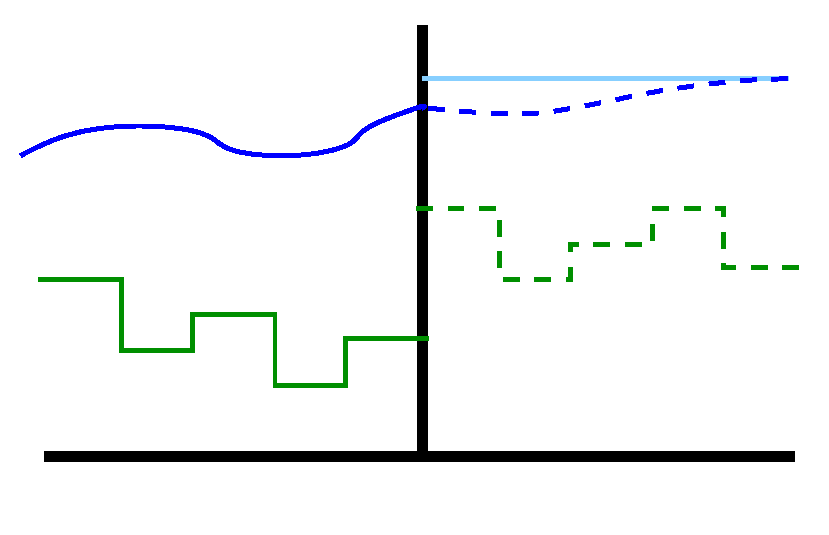
\includegraphics{mpc/MPC_gen}%
\end{picture}%
\setlength{\unitlength}{4144sp}%
%
\begingroup\makeatletter\ifx\SetFigFont\undefined%
\gdef\SetFigFont#1#2#3#4#5{%
  \reset@font\fontsize{#1}{#2pt}%
  \fontfamily{#3}\fontseries{#4}\fontshape{#5}%
  \selectfont}%
\fi\endgroup%
\begin{picture}(6051,3819)(2713,-7190)
\put(2881,-4111){\makebox(0,0)[lb]{\smash{{\SetFigFont{20}{24.0}{\familydefault}{\mddefault}{\updefault}{\color[rgb]{0,0,0}Outputs}%
}}}}
\put(3241,-7081){\makebox(0,0)[lb]{\smash{{\SetFigFont{20}{24.0}{\familydefault}{\mddefault}{\updefault}{\color[rgb]{0,0,0}$\gets$ Past}%
}}}}
\put(2971,-5191){\makebox(0,0)[lb]{\smash{{\SetFigFont{20}{24.0}{\familydefault}{\mddefault}{\updefault}{\color[rgb]{0,0,0}Inputs}%
}}}}
\put(6391,-3751){\makebox(0,0)[lb]{\smash{{\SetFigFont{20}{24.0}{\familydefault}{\mddefault}{\updefault}{\color[rgb]{0,0,0}Setpoint}%
}}}}
\put(6661,-7081){\makebox(0,0)[lb]{\smash{{\SetFigFont{20}{24.0}{\familydefault}{\mddefault}{\updefault}{\color[rgb]{0,0,0}Future $\to$}%
}}}}
\put(5401,-4921){\makebox(0,0)[lb]{\smash{{\SetFigFont{20}{24.0}{\rmdefault}{\mddefault}{\updefault}{\color[rgb]{0,0,0}$u$}%
}}}}
\put(5491,-7081){\makebox(0,0)[lb]{\smash{{\SetFigFont{20}{24.0}{\familydefault}{\mddefault}{\updefault}{\color[rgb]{0,0,0}$k=0$}%
}}}}
\put(5941,-4381){\makebox(0,0)[lb]{\smash{{\SetFigFont{20}{24.0}{\rmdefault}{\mddefault}{\updefault}{\color[rgb]{0,0,0}$y$}%
}}}}
\end{picture}%
}}
\caption{Rolling horizon optimization.}
\label{fig:mpc:mpc_gen}
\end{figure}

Model predictive control technology has two important aspects that are
interconnected. First, is the design of the online optimization
problem that is solved. The design must account for the control
objectives, process constraints and dynamics. Second, is the study of the injected
control moves in the plant. Since only the first input of the optimal
input sequence is used, it is important to provide guarantees that the
control objectives are met in the closed-loop. Stability theory
provides controller design guidelines and theoretical support to
ensure desirable closed-loop behavior by using the rolling horizon
optimization framework.

This chapter is organized as follows. In Section
\ref{sec:mpc:centralized}, we provide an overview of centralized 
MPC. We discuss optimal MPC in Section
\ref{sec:mpc:centralized:optimal} and suboptimal MPC in Section
\ref{sec:mpc:centralized:suboptimal}. In Section
\ref{sec:mpc:distributed}, we introduced distributed MPC; with
noncooperative MPC discussed in Section
\ref{sec:mpc:distributed:ncoop} and cooperative MPC discussed in
Section \ref{sec:mpc:distributed:coop}. An algorithm for robust
cooperative control is presented in Section \ref{sec:mpc:robust}. In
Section \ref{sec:mpc:related}, we discuss related 
work in the field of cooperative/ distributed MPC.  
Since the focus of this thesis is the
application of control technology for supply chain optimization, we
focus our attention on linear models in this section. In Chapter
\ref{chap:sc}, we show that the supply chain dynamics can be described
by linear models. 

\section{Centralized MPC}
\label{sec:mpc:centralized}
\subsection{Preliminaries}
We consider the linear system 
\begin{equation}
\label{eq:mpc:cent_model}
x^+ = Ax + Bu
\end{equation}
in which $x \in \mathbb{R}^n$, $u \in \mathbb{R}^m$ are the states and
inputs while $x^+$ is the successor state.

The system is constrained by the state constraint $x \in \mathbb{X}
\subseteq \mathbb{R}^n$ and input constraint $u \in \mathbb{U}
\subset \mathbb{R}^m$.

For a given finite horizon $N$, we define the input sequence as $\bu =
\left(u(0),u(1),\ldots,u(N-1)\right) \in \mathbb{U}^N$. The state at
time $j \geq 0$ for a system starting at state $x$ at time $j=0$,
under control $\bu$ is given by $\phi(j;x,\bu)$. If there is no
ambiguity, $\phi(j;x,\bu)$ is also denoted as $x(j)$. 

We define the tracking stage cost as $\ell(x,u) = 1/2(x'Qx + u'Ru); Q,R>0 $.  We define an economic state cost $\ell_E(x,u)$ in
Chapter \ref{chap:esc}. Without loss of generality, we assume
that the MPC is designed to track $(x,u)$ to the origin. For systems
in which the 
steady state  is not the origin, we can modify $\ell(x,u)$ by a
simple variable transformation $x \leftarrow x-x_s$, in which $x_s$ is
the steady state  of choice. We also define a terminal cost on the
state, $V_f(x) = 1/2x'Px, P>0$. An important feature of the MPC online optimization problem is the
terminal constraint \eqref{eq:mpc:Xfconst}. The set $\mathbb{X}_f
\subseteq \mathbb{X}$ is the terminal set.

The MPC online optimization problem is now defined as:
\begin{xalignat}{2}
\mathbb{P}_N(x):& \min_{\bu}V_N(x,\bu) & \nonumber \\
&\text{s.t.~} x(j+1) = Ax(j) + Bu(j), &  j =
\set{0,1,2,\ldots,N-1} \nonumber \\
&x(j) \in \mathbb{X} &  j  = \set{0,1,2,\ldots,N} \nonumber\\
&u(j) \in \mathbb{U} &  j =
\set{0,1,2,\ldots,N-1} \label{eq:mpc:PNx} \\
&x(0) = x & \nonumber\\
&x(N) \in \mathbb{X}_f \label{eq:mpc:Xfconst}
\end{xalignat}

In the optimization problem $\mathbb{P}_N(x)$, the cost function
$V_N(x,\bu)$ is given by:
\begin{equation}
\label{eq:mpc:VN}
V_N(x,\bu) = \sum_{j=0}^{N-1} \ell(x(j),u(j)) + V_f(x(N))
\end{equation}




The set $\mathbb{Z}_N$ is defined as the set of $(x,\bu)$ for which the
problem $\mathbb{P}_N(x)$ is feasible. That is,
\begin{equation}
\label{eq:mpc:Z}
\mathbb{Z}_N := \set{(x,\bu) \mid \phi(j;x,\bu) \in \mathbb{X},
  \phi(N;x,\bu) \in \mathbb{X}_f, \bu \in \mathbb{U}^N}
\end{equation}

The projection of set $\mathbb{Z}_N$ onto $\mathbb{X}$ is the set of
admissible states, denoted by $\mathcal{X}_N$. That is, 
\begin{equation}
\label{eq:mpc:X_N}
\mathcal{X}_N := \set{ x \mid \exists \bu \in \mathbb{U}^N,
  \text{~s.t~} (x,\bu) \in \mathbb{Z}_N}
\end{equation}

For a given $x \in \mathcal{X}_N$, the set of feasible inputs is
given by $\mathcal{U}_N(x)$:
\begin{equation}
\label{eq:mpc:U_Nx}
\mathcal{U}_N(x) := \set{ \bu \mid (x,\bu) \in \mathbb{Z}_N}
\end{equation}

The online optimization problem can now succinctly be expressed as:
\[ \mathbb{P}_N(x) := \min_{\bu}{V_N(x,\bu)} \qquad \text{s.t.~} \bu
\in \mathcal{U}_N(x) \]

\subsection{Optimal MPC}
\label{sec:mpc:centralized:optimal}
The following assumptions are made on the system:
\begin{assumption}
\label{ass:mpc:stab}
The centralized system $(A,B)$
is stabilizable.  
\end{assumption}

\begin{assumption}
\label{ass:mpc:psd}
The cost functions $\ell(x,u)$ and $V_f(x)$ are positive definite
\footnote{ A function $f(x)$ is positive definite if $f(x) \geq 0
  \forall x$ and $f(x) = 0$ if and only if $x = 0$.}
\end{assumption}
\begin{assumption}
\label{ass:mpc:bsa}
The set $\mathbb{X}_f$ and the  costs $\ell(x,u), V_f(x)$ are chosen
such that there exists a terminal controller $u = \kappa_f(x)$
that satisfies: 
\begin{xalignat}{1}
\label{eq:mpc:bsa}
V_f(Ax+B\kappa_f(x)) -V_f(x) \leq -\ell(x,\kappa_f(x)) &\qquad \forall x
\in \mathbb{X}_f \\
Ax + B\kappa_f(x) \in \mathbb{X}_f,  \kappa_f(x) \in \mathbb{U}& \qquad
\forall x \in \mathbb{X}_f
\end{xalignat}
\end{assumption} 

\begin{assumption}
\label{ass:mpc:closed}
The set $\mathbb{U}$ is convex, closed and compact and contains the origin in
its interior. The set $\mathbb{X}$ is convex, closed and contains the origin
in its interior. The set $\mathbb{X}_f$ is  convex, closed, compact and
contains the origin in its interior.
\end{assumption}

\begin{remark}
The choice of quadratic stage and terminal costs with $Q > 0, R >0,
P>0$ automatically satisfies Assumption \ref{ass:mpc:psd}.
\end{remark} 

\begin{remark}
From Assumption \ref{ass:mpc:stab}, we know that there exists a linear
feedback $K$ such that $(A+BK)$ is stable. In other words, the
closed-loop $x^+ = (A+BK)x$ is stable. We choose such a $K$ as the
terminal controller $\kappa_f(x)$. The terminal penalty $V_f(x) =
x'Px$ is chosen as 
the solution to the Lyapunov equation (which exists as a consequence
of Assumption \ref{ass:mpc:psd}):
\[ (A+BK)'P(A+BK) + (Q+K'RK) = P \]

For the pair $(P,K)$, we can define the control invariant region in
the state-space in which $u=Kx$ does not activate any constraints as:
\[ \mathbb{X}_f := \set{x \mid x(i) = (A+BK)^ix \in \mathbb{X}_f \subseteq
  \mathbb{X}, Kx(i) \in \mathbb{U}, \forall i \geq 0}
\]

For linear systems, such sets can be easily constructed. See
\citet{gilbert:tan:1991} for an algorithm. 
\end{remark}

The optimal solution to the optimization problem  \eqref{eq:mpc:PNx}
is denoted by 
$\bu^0(x)$ and the optimal objective value is given by $V_N^0(x)$. The
optimal-MPC control law is now defined as $\kappa_o(x) = u^0(0;x)$ in
which $u^0(0;x)$ is the first input in the optimal sequence
$\bu^0(x)$. The closed-loop evolution, under the control law
$\kappa_0(x)$ is $x^+ = Ax + B\kappa_0(x)$. The centralized optimal
MPC asymptotic (exponential) stability theorem is presented below. This theorem is
attributed to \citet[Thm 2.24(b), Chap. 2]{rawlings:mayne:2009}.

\begin{theorem}[Optimal MPC stabilty]
\label{thm:mpc:optimal}
Let Assumptions \ref{ass:mpc:stab}--\ref{ass:mpc:closed} hold. Then
the origin is exponentially stable with a region of attraction
$\mathcal{X}_N$ for the system $x^+ = Ax + B\kappa_0(x)$. If
$\mathcal{X}_N$ is unbounded, then the region of attraction is any
sublevel set of $V_N^0(\cdot)$.
\end{theorem}

The detailed technical proof for Theorem \ref{thm:mpc:optimal} is
provided in \citet[Chap. 2]{rawlings:mayne:2009}. We provide a sketch
of the proof below for linear systems with positive definite stage
cost. The stability proof follows by establishing that 
$V_N^0(\cdot)$ is a 
Lyapunov function for the closed-loop dynamics $x^+=Ax +
B\kappa_0(x)$. 

Lyapunov stability theorem for a dynamic system
$z^+=f(z)$ states that if a function $V(z)$ exists with the following
properties
\begin{gather}
V(z) \geq \alpha_1(\norm{z}), \qquad \forall z \in \mathcal{Z} \label{eq:mpc:lyap:lower-bound} \\
V(z) \leq \alpha_2(\norm{z}), \qquad \forall z \in \mathcal{Z} \label{eq:mpc:lyap:upper-bound}\\
V(z^+) -V(z) \leq -\alpha_3(\norm{z}) \qquad \forall z \in \mathcal{Z} \label{eq:mpc:lyap:cost-drop}
\end{gather}
in which $\alpha_i(\cdot), i \in \set{1,2,3}$ are
$\mathcal{K}_{\infty}$ functions\footnote{A function $\sigma: \mathbb{R}_+
  \rightarrow \mathbb{R}_+$ belongs to the class of
  $\mathcal{K}_{\infty}$ functions if $\sigma$ is continuous, strictly
increasing, $\sigma(0) = 0$ and $\sigma(s) \rightarrow \infty$ as $s
\rightarrow \infty$.}; then the origin is asymptotically
stable on the set $\mathcal{Z}$. Converse Lyapunov theorem states that if the dynamic system is
asymptotically stable, then there exists a Lyapunov function for that
system. If the $\mathcal{K}_{\infty}$ functions $\alpha_i$  are of the
form $\lambda_i \norm{x}^\sigma, \lambda_i,\sigma >0$, then the dynamic
system is exponentially stable (see \citet[Appendix B.]{rawlings:mayne:2009} for precise
statements).

To show that $V_N^0(\cdot)$ is a Lyapunov function for the linear
system under study \footnote{refer to \citet[Chap
  2.]{rawlings:mayne:2009} for more general cases}, we first define
the warm start as follows:
\begin{definition}[Warm Start]
\label{def:mpc:warmstart}
Let $(x,\bu)$ be a state-input vector pair such that $(x,\bu) \in
\mathbb{Z}_N$. Then the warm start for the successor initial state
$x^+ = Ax+B\bu(0;x)$ is defined as:
\begin{equation*}
%\label{eq:warmstart}
\tilde{\bu} = \left (\bu(1;x),\bu(2;x),\ldots,\bu(N;x),u_+\right)
\end{equation*}
in which  $u_+ = \kappa_f(\phi(N;x,\bu))$.
\end{definition}

The lower bound  \eqref{eq:mpc:lyap:lower-bound} for the optimal
function is established by using the 
fact that we choose $Q,R,P>0$ (Assumption \ref{ass:mpc:psd}). By this choice of $Q,R,P$, $V_N(x,\bu)$
is positive definite, and hence $V_N^0(x) \geq
\ell(x,\kappa_0(x))$. Since $\ell(x,u) = 1/2(x'Qx+u'Ru)$, we have that
$\ell(x,u) \geq 1/2x'Qx \geq 1/2\underline{\lambda}_Q\norm{x}^2$. The last
inequality follows from the positive definiteness of $Q$ with
$\underline{\lambda}_Q >0$ denoting the smallest eigen-value of
$Q$. We denote the smallest and largets eigen-value of a matrix
$\mathcal{H}$ by $\underline{\lambda}_\mathcal{H}$ and
$\overline{\lambda}_{\mathcal{H}}$ respectively.

Following the definition of the warm start and an optimal input
sequence $\bu^0(x)$, the warm start $\tilde{\bu}^0$ is feasible for
the successor state $x^+ = Ax+B\kappa_o(x)$, because $x(N) = \phi(N;x,\bu^0)$
belongs to $\mathbb{X}_f$ (and hence $Ax(N)+B\kappa_f(x(N)) \in
\mathbb{X}_f$ by Assumption \ref{ass:mpc:bsa}). Therefore, we get the
following inequality that establishes the cost-drop property in
Equation \eqref{eq:mpc:lyap:cost-drop}.
\begin{gather*}
V_N(x^+,\tilde{\bu}^0) =
V_N^0(x)+\underbrace{\left(V_f(Ax(N)+B\kappa_f(x(N)))
+\ell(x(N),\kappa_f(x(N)))-V_f(x(N))\right)}_{\leq
  0 \text{~by Assumption \ref{ass:mpc:bsa}}} -
\underbrace{\ell(x,\kappa_0(x))}_{\geq 0 \text{~by Assumption
    \ref{ass:mpc:psd}}} \\
V_N^0(x^+) \leq V_N(x^+,\tilde{\bu}^0)\leq  V_N^0(x)
 - \underline{\lambda}_{Q}\norm{x}^2
\end{gather*}

The upper bound \eqref{eq:mpc:lyap:upper-bound} is established by
showing that $V_N^0(x) \leq V_f(x) 
\leq \overline{\lambda}_P\norm{x}^2,
\forall x \in \mathbb{X}_f$. To do so, consider $x \in \mathbb{X}_f$
and choose $u(0) = \kappa_f(x)$. Therefore, $x(1) = Ax+Bu(0)$
satisfies $V_f(x(1))+\ell(x,u(0)) \leq V_f(x)$. Since Assumption
\ref{ass:mpc:bsa} is satisfied, we can choose $u(1) =
\kappa_f(x(1))$ to obtain $x(2) = Ax(1) + Bu(1)$. Therefore
$V_f(x(2))+\ell(x(1),u(1)) \leq V_f(x(1))$. So, we can conclude that
$V_f(x(2))+\ell(x(1),u(1))+\ell(x,u(0)) \leq V_f(x(1))+\ell(x,u(0))
\leq V_f(x)$, using the first inequality. In such a manner, we can
construct an input sequence $\bu_{\kappa_f}(x) := \set{u(j) =
  \kappa_f(x(j))}$, so 
that $V_N(x,\bu_{\kappa_f}) \leq V_f(x)$. Since $\bu_{\kappa_f}$ is a
feasible input sequence, the optimal cost function $V_N(x,\bu^0) \leq
V_N(x,\bu_{\kappa_f}) \leq V_f(x), \forall x \in \mathbb{X}_f$
\citep{pannocchia:rawlings:wright:2011}.  
The upper bound is extended to $\mathcal{X}_N$ using the
compactness of $\mathbb{X}_f$ \citep[Proposition 2.18]{rawlings:mayne:2009}. 

\subsection{Suboptimal MPC}
\label{sec:mpc:centralized:suboptimal}
The favorable properties of the closed-loop was established in optimal
MPC based on the optimal value function. However, in many practical
applications, we might not be able to solve the optimization problem
\eqref{eq:mpc:PNx} to optimality. We might not be able to solve to
optimality in the given sample time (for large 
problems and small sampling time) or by design (like for
example, in cooperative MPC, as we show in Section
\ref{sec:mpc:distributed:coop}). Hence, it is important that asymptotic
stability be ensured when the online optimizations do not converge to
the optimal solution. Suboptimal MPC theory is used to establish this
property. 

Given any feasible input sequence $\bu \in \mathcal{U}_N(x)$ for the
state $x$, the warm start is defined according to Definition
\ref{def:mpc:warmstart}, and the successor input set for the state
$x^+=Ax+Bu(0;x)$ is defined as
below:
\begin{definition}[Successor input set]
\label{def:mpc:successor-input-set}
Consider $(x,\bu)$ such that $\bu$ is feasible for
$\mathbb{P}_N(x)$ \eqref{eq:mpc:PNx}.  For the  successor state 
$x^+ = Ax+Bu(0;x)$, we define the set $G(x,\bu)$
\begin{equation}
\label{eq:mpc:succesor-input-set}
G(x,\bu) = \lbrace \bu^+ \mid \bu^+ \in
\mathcal{U}_N(x^+), V_N(x^+,\bu^+)\leq V_N(x,\tilde{\bu}), 
V_N(x^+,\bu^+) \leq V_f(x^+) \text{~if~} x\in \mathcal{B}_r \subset \mathbb{X}_f \rbrace
\end{equation}
in which $\tilde{\bu}$ is the warm start given by Definition 
\ref{def:mpc:warmstart} and $\mathcal{B}_r$ is a ball of radius $r>0$. We
choose $r$ sufficiently small such that  
$\mathcal{B}_r$ is a subset of the terminal region.  
\end{definition}

Similar to optimal MPC, we inject the first input from the suboptimal
sequence to the plant. The control law in the case of suboptimal MPC
is therefore a set, as any input sequence in the successor input set
can be used. The closed-loop analysis, consequently is on the
evolution of the following system
\begin{align}
x^+ &= Ax+ B\kappa_s(x) \label{eq:mpc:suboptimal:xcl} \\
\bu^+ &\in G(x,\bu)  \label{eq:mpc:suboptimal:ucl}
\end{align}
in which $\kappa_s(x)$ is the control law given by the first input in
the input sequence $\bu(x)$. The following theorem, attributed to
\citet{pannocchia:rawlings:wright:2011} establishes the exponential
stability of suboptimal MPC. Additionally, we make the 
following assumptions on the cost function $V_N(x,\bu)$.

\begin{assumption}
\label{ass:mpc:suboptimalconstants}
There exist positive constants $a,a_1',a_2',a_f$ and $r$, such
that the cost function $V_N(x,\bu)$ satisfies:
\begin{alignat*}{2}
\ell(x,u) &\geq a_1' \norm{(x,u)}^a &\qquad (x,u) &\in \mathbb{X} \times \mathbb{U} \\
V_N(x,\bu) &\leq a_2' \norm{(x,\bu)}^a &\qquad (x,u) &\in
\mathcal{B}_{r} \\
V_f(x) &\leq a_f\norm{x}^a &\qquad x &\in \mathbb{X}
\end{alignat*}
in which $\mathcal{B}_{r}$ is the ball of radius $r$.
\end{assumption}

Note that it is easy to show that Assumption
\ref{ass:mpc:suboptimalconstants} is satisfied for linear systems and
quadratic costs.

\begin{theorem}
\label{thm:mpc:suboptimal}
Let Assumptions \ref{ass:mpc:stab} -- \ref{ass:mpc:closed} and
\ref{ass:mpc:suboptimalconstants} 
hold. For any $x$ for which  $\mathcal{U}_N(x)$  is not empty, choose
$\bu \in \mathcal{U}_N(x)$. Then, the origin of the closed-loop system 
\eqref{eq:mpc:suboptimal:xcl}--\eqref{eq:mpc:suboptimal:ucl}
is asymptotically stable on (arbitrarily large) compact  subsets of
the feasible region $\mathcal{X}_N$
\end{theorem}

We now provide a sketch of the proof for Theorem
\ref{thm:mpc:suboptimal} for linear systems with quadratic,
positive-definite stage costs. We refer the reader to
\citet{pannocchia:rawlings:wright:2011} for  the detailed proof
of a more general case. 
Since in suboptimal MPC, there are multiple input sequences that satisfy
\eqref{eq:mpc:succesor-input-set}, the closed-loop dynamics follows a
difference inclusion, instead of a difference equation. Using the
notation $z = (x,\bu)$ (called as the extended state), the closed-loop
\eqref{eq:mpc:suboptimal:xcl}--\eqref{eq:mpc:suboptimal:ucl} can be
succinctly written as:
\[ z^+ \in H(z) := \set{(x^+,\bu^+) \mid x^+\in Ax+B\kappa_s(x), \bu^+ \in
  G(z)} \]

Analogous to the Lyapunov function described in the previous section;
we can write a Lyapunov function for the difference inclusion. $V(z)$
is an exponential Lyapunov function for $z^+\in H(z)$ on the set
$\mathcal{Z}$ if the following hold, with $a_1,a_2,a_3,a \geq 0$ \citep[Definition
13]{pannocchia:rawlings:wright:2011}. 
\begin{xalignat}{1}
V(z) \geq a_1\norm{z}^a,& \qquad \forall z \in
\mathcal{Z} \label{eq:mpc:Dlyap:lower-bound} \\ 
V(z) \leq a_2\norm{z}^a, &\qquad \forall z \in
\mathcal{Z} \label{eq:mpc:Dlyap:upper-bound}\\ 
\max_{z^+ \in H(z)}{V(z^+)} -V(z) \leq -a_3\norm{z}^a,&  \qquad \forall z \in
\mathcal{Z} \label{eq:mpc:Dlyap:cost-drop} 
\end{xalignat}

Exponential stability is established by showing that $V_N(x,\bu)$ is a
Lyapunov function for the difference inclusion $z^+ \in H(z)$. 
To show that the cost function $V_N(x,\bu)$ satisfies
\eqref{eq:mpc:Dlyap:lower-bound}--\eqref{eq:mpc:Dlyap:upper-bound}, we
proceed by noting that the cost function can be written as:
\begin{equation}
V_N(x,\bu) = \frac{1}{2} \begin{bmatrix} x\\\bu \end{bmatrix}'
\mathcal{H} \begin{bmatrix} x\\\bu \end{bmatrix}  
\qquad 
\mathcal{H} = \begin{bmatrix} \mathcal{A}'\mathcal{Q}\mathcal{A}
  &\mathcal{A}'\mathcal{Q}\mathcal{B}\\
  \mathcal{B}'\mathcal{Q}\mathcal{A} &
  \mathcal{B}\mathcal{Q}\mathcal{B} + \mathcal{R} \end{bmatrix} 
\label{eq:mpc:VN_H}
\end{equation}
in which 
\begin{equation*}
\begin{bmatrix}x(0)\\x(1)\\\vdots\\x(N)\end{bmatrix} =
\underbrace{\begin{bmatrix}I\\A\\\vdots\\A^{N-1}\end{bmatrix}}_{\mathcal{A}}x
+\underbrace{\begin{bmatrix}0&0&\ldots&0\\
B&0&\ldots&0\\AB&B&\ldots&0\\
\vdots&\vdots&\ddots&\ldots\\
A^{N-1}B&A^{N-2}B&\ldots&B\end{bmatrix}}_{\mathcal{B}}\bu  
\end{equation*}
and $\mathcal{Q} = \diag(\underbrace{Q,Q,\ldots,Q}_{N-1 
  \text{~times}},P)$ and $\mathcal{R} =
\diag(\underbrace{R,R,\ldots,R}_{N \text{~times}})$. 
Since $Q,R>0$, the matrix $\mathcal{H}$ is a positive definite
matrix. Therefore, $1/2\underline{\lambda}_{\mathcal{H}}\norm{x,\bu}^2
\leq V_N(x,\bu) \leq \overline{\lambda}_{\mathcal{H}}\norm{x,\bu}^2$
Thus,
\eqref{eq:mpc:Dlyap:lower-bound} and \eqref{eq:mpc:Dlyap:upper-bound}
are satisfied. To show the cost-drop property, notice that for $x \in
\mathcal{B}_r \subset \mathbb{X}_f$, we have by the property of
$G(x,\bu)$ that $V_N(x,\bu) \leq V_f(x)$. As shown in the previous
section, $V_f(x) = 1/2x'Px \leq \overline{\lambda}_P\norm{x}^2$. Hence,
we have that 
\begin{equation}
\label{eq:mpc:suboptimal:inputcost0}
\underline{\lambda}_{\mathcal{H}}\norm{\bu}^2 \leq \underline{\lambda}_{\mathcal{H}}\norm{(x,\bu)}^2 \leq V_N(x,\bu)
\leq V_f(x) \leq  \overline{\lambda}_P\norm{x}^2 ,\qquad x \in
\mathcal{B}_r
\end{equation}
From the inequality \eqref{eq:mpc:suboptimal:inputcost0}, we can conclude that 
\begin{equation}
\label{eq:mpc:suboptimal:inputcost1}
\norm{\bu} \leq d
\norm{x}, \quad x \in \mathcal{B}_r
\end{equation}
in which $d =
\sqrt{\frac{\overline{\lambda}_P}{\underline{\lambda}_{\mathcal{H}}}}$. Using
 inequality \eqref{eq:mpc:suboptimal:inputcost1}, we can establish
 that
\begin{equation}
\label{eq:mpc:suboptimal:inputcost2}
\norm{(x,\bu)} \leq
\norm{x}+\norm{\bu} \leq (1+d)\norm{x} \leq (1+d)\norm{(x,u(0))}
\qquad x \in \mathcal{B}_r
\end{equation}
As we saw in the previous section, $V_N(x^+,\tilde{\bu})-V_N(x,\bu) \leq
-\ell(x,u(0))$ (by choice of the warm start). Since, $\bu^+ \in G(x,\bu)$ implies that (i)
$\bu^+$ drives the state $x^+$ into the terminal region in $N$ steps
and, (ii) ensures that the cost of doing so is less than
$V_N(x^+,\tilde{\bu})$; we can conclude that
\[V_N(x^+,\bu^+)-V_N(x,\bu) \leq -\ell(x,u(0))\]
Note that the lower
bound of $\ell(x,u(0))$ is given by
\[1/2\min{(\underline{\lambda}_Q,\underline{\lambda}_R)}\norm{(x,u(0))}^2
\leq  \ell(x,u(0))\]
Denote $1/2\min{(\underline{\lambda}_Q,\underline{\lambda}_R)} =
a_1'$. Using the inequality \eqref{eq:mpc:suboptimal:inputcost2}, we
can then conclude that 
\[ V_N(x^+,\bu^+)-V_N(x,\bu) \leq -\ell(x,u(0)) \leq
-a_1'\norm{(x,u(0))}^2 \leq \frac{-a_1'}{(1+d)^2}\norm{x,\bu}^2 ,\qquad
\forall x \in \mathcal{B}_r\]

The cost-drop property can be extended to the region of attraction
using compactness of $\mathbb{U}$.

The online optimization problem being solved for suboptimal MPC is 
slightly modified from that of optimal MPC. In Equation
\eqref{eq:mpc:suboptimal:PNx}, we present the optimization problem for
suboptimal MPC.

\begin{equation}
\label{eq:mpc:suboptimal:PNx}
\mathbb{P}_N(x) := \min_{\bu}{V_N(x,\bu)} \qquad \text{s.t.~} \bu
\in \mathcal{U}_N(x), \norm{\bu} \leq d \norm{x}, \text{if~} x \in
\mathcal{B}_r
\end{equation}

For future reference, we define the following set:
\begin{equation}
\label{eq:mpc:UN_sub}
\mathcal{U}_N^{s}(x;r) := \set {u \mid u \in \mathcal{U}_N(x),\norm{\bu} \leq d \norm{x}, \text{if~} x \in
\mathcal{B}_r}
\end{equation}

Note that the constraint on $\norm{\bu}$ is not enforced in practical
implementations as $r>0$ can be chosen arbitrarily small. 

The advantage of using suboptimal MPC is that the we do not have to
wait for the online optimizations to 
converge; and we can inject any suboptimal iterate generated by the
optimization algorithm into the plant as long as that iterate belongs
to the set $G(x,\bu)$. Another important feature that stands out from
the suboptimal MPC theory is that just using the warm start at every
time ensures exponential stability. Online optimization improves the
open-loop prediction cost.\footnote{But we cannot say anything about
  the closed-loop cost if we stop at suboptimal iterates.}




\section{Distributed MPC}
\label{sec:mpc:distributed}
In the previous sections, we introduced centralized MPC, in which a
single controller is designed for the system. The centralized
controller uses system-wide information about models, constraints on
the inputs and states, and objective to find a control law that has favorable properties. In many practical
applications, this centralized information is distributed among many
agents. For example, a chemical plant may have multiple MPC
controllers running, each of which is controlling one process in the
facility. In such cases, it is important to study how to coordinate
information spread among multiple controllers to better control the
plant. Distributed MPC is the study of various architectures for
information sharing and retrieval to coordinate multiple controllers
\citep{scattolini:2009}. 

In this Section, we first introduce the models and objectives of each
agent or node in the system in Section
\ref{sec:mpc:distributed:models}. In Section \ref{sec:mpc:distributed:ncoop}, we describe the
so-called noncooperative MPC, in which the nodes share information
regarding their future (predicted) input moves with each other. In Section
\ref{sec:mpc:distributed:coop}, we present the cooperative MPC
algorithm in which the nodes not only share information about their
predicted input moves with each other, but they also share (and use)
model and objective functions. We show that cooperative MPC is an
implementation of suboptimal centralized MPC, and hence it inherits
all the desirable properties of suboptimal (centralized) MPC. 
We   present a simple  two-tank system shown in Figure
\ref{fig:2tankunstable} in Section
\ref{sec:mpc:distributed:example}. We use this example to illustrate
the key properties of distributed
MPC algorithms, namely (i) noncooperative MPC can de-stabilize a
plant, and (ii) with careful design, cooperative MPC can stabilize any
plant that can be stabilized using centralized MPC. We choose the two-tank system
because its model is a system of integrators like the supply chain
model (see Chapter \ref{chap:sc}).
 
\subsection{Models, constraints and objective functions}
\label{sec:mpc:distributed:models}
In distributed MPC, the system is assumed to be composed of several
subsystems (or agents or nodes). We use the index $i$ to denote a
subsystem, and $M$ to denote the total number of subsystems. Each
subsystem $i \in \set{1,2,3,\ldots,M}$ has the following dynamics
and constraints:
\begin{gather}
\label{eq:mpc:distributed:dynamics}
x_i^+ = A_i x_i + B_{ii} u_i + \sum_{l \in \set{1,2,\ldots,M} \atop l \neq i}
B_{il} u_l \\
x_i \in \mathbb{X}_i \qquad u_i \in
\mathbb{U}_i \label{eq:mpc:distributed:constraints} 
\end{gather}
in which $x_i,u_i$ are the states and inputs in subsystem $i$.

The stage cost for a subsystem is given by:
\begin{equation}
\label{eq:mpc:distributed:stage-cost}
\ell_i(x_i,u_i) = 1/2(x_i'Q_ix_i + u_i'R_iu_i)
\end{equation}
with the penalties $Q_i,R_i >0$. 

The centralized (system-wide) model is therefore:
\begin{gather}
\label{eq:mpc:distributed:cent}
\begin{bmatrix}x_1\\x_2\\\vdots\\x_M\end{bmatrix}^+
= \underbrace{\begin{bmatrix}A_1 & & & \\ & A_2 & & \\ & & \ddots& \\
    & & & A_M \end{bmatrix}}_{A}
\underbrace{\begin{bmatrix}x_1\\x_2\\\vdots\\x_M\end{bmatrix}}_{x}+
\underbrace{\begin{bmatrix}B_{11}&B_{12}&\ldots&B_{1M}\\
B_{21}&B_{22}&\ldots&B_{2M}\\ 
\vdots& \vdots& \ddots& \vdots\\
B_{M1}&B_{M2}& \ldots&B_{MM} \end{bmatrix}}_{B}
\underbrace{\begin{bmatrix}u_1\\u_2\\\ldots\\u_M\end{bmatrix}}_{u} \\
\mathbb{X} = \mathbb{X}_1 \times \mathbb{X}_2 \times \ldots \times
\mathbb{X}_M \\
\mathbb{U} = \mathbb{U}_1 \times \mathbb{U}_2 \times \ldots \times
\mathbb{U}_M
\end{gather}

The centralized stage-cost is 
\begin{equation}
\label{eq:mpc:distributed:cent-stage-cost}
\ell(x,u) = \sum_{i=1}^{M} \ell_i(x_i,u_i)
\end{equation}

We do not make any special assumptions on the local models
\eqref{eq:mpc:distributed:dynamics}--\eqref{eq:mpc:distributed:constraints}. The
only assumptions made are on the centralized model and stage costs
\eqref{eq:mpc:distributed:cent}--\eqref{eq:mpc:distributed:cent-stage-cost}. We
assume that the centralized model and stage costs satisfies Assumptions
\ref{ass:mpc:stab}--\ref{ass:mpc:closed} and \ref{ass:mpc:suboptimalconstants}. It is important to note that
the terminal controller $\kappa_f(\cdot)$, terminal cost $V_f(\cdot)$
and, terminal set $\mathbb{X}_f$ are all defined only for the
centralized system. 


\subsection{Noncooperative MPC}
\label{sec:mpc:distributed:ncoop}
In noncooperative MPC, each subsystem minimizes
its local objective function. Therefore, the subsystem optimization
problem $\mathbb{P}_N^i(x_i,\mathbf{v}_{-i})$ is given below. For subsystem $i$, we use
$-i$ to denote all the other subsystems, i.e.. $-i =
\set{1,2,\ldots,i-1,i+1,\ldots,M}$. 
\begin{xalignat}{2}
\mathbb{P}_{N,nc}^i(x_i;\mathbf{v}_{-i}):& \min_{\bu_i}{\sum_{j=0}^{N-1}
\ell_i(x_i(j),u_i(j)) + V_{f,i}(x_i(N))}& \nonumber\\
&\text{s.t.~} x_{i}(j+1) = A_{ii}x_i(j) + B_{ii}u_i(j) +  \sum_{l \in \set{1,2,\ldots,M} \atop l \neq i}
B_{il} v_l(j) & j = \set{0,1,\ldots,N-1} \nonumber\\
& x_i(j) \in \mathbb{X}_i & j = \set{0,1,\ldots,N-1}  \label{eq:mpc:distributed:ncoop:PNi}\\
& u_i(j) \in \mathbb{U}_i & j = \set{0,1,\ldots,N-1} \nonumber \\
&x_i(0) = x_i \nonumber
\end{xalignat}

We wish to bring the readers attention to two important features of
the ``local'' optimization problem $P_{N,nc}^i(x_i;\mathbf{v}_{-i})$,
 (i) to make accurate predictions of $x_i(j)$, and hence the
cost function, subsystem $i$
needs to know the future (predicted) inputs of all other subsystems,
and (ii) no terminal constraints are enforced \footnote{Although we
  include a terminal penalty, we provide no design methods to find
  a terminal penalty}. 

In noncooperative MPC (Algorithm \ref{alg:mpc:distributed:ncoop}), each
subsystem broadcasts its input sequence prediction. Based on this
prediction, every subsystem solves its local optimization problem. The
final input is a convex combination of the previously broadcast inputs
and the optimized inputs. 

%\begin{algo}[Noncooperative MPC]\mbox{ }
%\label{alg:mpc:distributed:ncoop}

\begin{algorithm}
  \KwData{Starting state $\set{x_i(0)}$, initial guess $\left(\tilde{\bu}_1(0),
    \tilde{\bu}_2(0),\ldots,\tilde{\bu}_M(0)\right)$, $\bar{p} \geq
  0$, $\omega_i \in (0,1)$ such that $\sum_{i=0}^{M}\omega_i = 1$}
  \KwResult{Closed loop $x(j),u(j)$, $j = \set{0,1,2,\ldots}$}
   Set $j \leftarrow 0$ \\
    \While {$j \geq 0$}{
      Set $p \leftarrow 0$\\
      Set $x_i \leftarrow x_i(j))$, for i in $1,2,\ldots,M$\\
      Set $\tilde{\bu}_i \leftarrow \tilde{\bu}_i(j)$, for i in $1,2,\ldots,M$\\
      Broadcast $\tilde{\bu}_i$ to all other subsystems for  i in
      $1,2,\ldots,M$\\
      Each subsystem $i$ creates $\tilde{\bu}_{-i}$ from the other
      subsystem inputs\\
      \While {$p < \bar{p}$}{
       Solve $\mathbb{P}_{N,nc}^{i}(x_i,\bu_{-i})$ to obtain
       $\bu_i^0$ for i in $1,2,\ldots,M$ \\
       Set $\bu_i^{(p+1)} \leftarrow \omega_i \bu_i^{(p)} +
       (1-\omega_i) \bu_i^0$ for  i in $1,2,\ldots,M$ \\
        Set $p \leftarrow p+1$\
   }
   Set input $u_i(j) = \bu_i(0)$ for i in $ 1,2,\ldots,M$ and
   broadcast \\
   Evolve state from $x_i(k)$ to $x_i(k+1)$ for the input just
   obtained \\
   Obtain feasible input $\tilde{\bu}_i(j+1)$ for i in $1,2,\ldots,M$\\
   Set $j \leftarrow j+1$
   }
\caption{Noncooperative MPC}
\label{alg:mpc:distributed:ncoop}
\end{algorithm}
%\end{algo}

In the inner loop of Algorithm \ref{alg:mpc:distributed:ncoop}, each
subsystem is finding its {\em{best response}} to the other subsystem
inputs. It can be shown that as $p \rightarrow \infty$, the
solutions $\bu_i^{(p)}$ converge to a point called the Nash
Equilibrium \citep{basar:olsder:1999}. As has been shown earlier by
\citet[Sec 4.3.1]{venkat:2006}, the Nash equilibrium may be
unstable. We also wish to point out that we cannot make any claims
about the feasibility of $\mathbb{P}_N^i(x_i;\mathbf{v}_{-i})$ in the
inner optimization loop of the noncooperative MPC algorithm. For
similar reasons, we cannot make any claims about how to obtain
$\tilde{\bu}_i(j+1)$.

In Figure \ref{fig:mpc:unstable}, we show the unstable closed-loop response using Algorithm
\ref{alg:mpc:distributed:ncoop} for a simple two-tank example.

\subsection{Cooperative MPC}
\label{sec:mpc:distributed:coop}
In this section, we tailor the distributed MPC algorithm to be an
implementation of suboptimal MPC. To do so, we require that the
subsystems not only share input forecasts, but also model, constraints
and objective functions with each other. Under this requirement, the
cooperative MPC optimization problem is written as:

\begin{equation}
\label{eq:mpc:distributed:coopPNx}
\mathbb{P}_N(x) := \min_{\bu}{V_N(x,\bu)} \qquad \text{s.t.~} \bu
\in \mathcal{U}^s_N(x;r)
\end{equation}

Note that the cooperative MPC optimization problem is the same as the
suboptimal MPC optimization problem. The cooperative MPC algorithm is
presented in Algorithm \ref{alg:mpc:distributed:coop}.

%\begin{algo}[Cooperative MPC] \mbox{ }
%\label{alg:mpc:distributed:coop}

\begin{algorithm}
 \KwData{Starting state $x(0)$, initial guess
   $(\tilde{\bu}_1(0),\tilde{\bu}_2(0),\ldots,\tilde{\bu}_M(0)) \in \mathcal{U}^s_N(x(0);r)$,
   $\bar{p} \geq 1$ and $\omega_i \in (0,1)$ such that
   $\sum_{i=0}^{M}\omega_i = 1$}
 \KwResult{Closed loop $(x(j),u(j)), j = \set{1,2,\ldots}$}
 set $j \leftarrow 0$ \\
 \While {$j \geq 0$}{
   Set $p \leftarrow 0$, $x \leftarrow x(j)$\\
   Set $\bu_i^{(p)} \leftarrow \tilde{\bu}_i(j)$ for $i = 1,2,\ldots,M$\\
   Broadcast current subsystem inputs $\tilde{\bu}_i(j)$ to other
   subsystems \\
   \While {$p < \bar{p}$}{
       Solve $\min_{\bu_i}{V_N(x,\bu)} \quad \text{s.t.~} \bu \in
       \mathcal{U}_N^s(x;r); \bu_{-i} = \bu_{-i}^{(p)}$ to obtain
       $\bu_i^0$ for i in $1,2,\ldots,M$ \\
       Set $\bu_i^{(p+1)} \leftarrow \omega_i \bu_i^{(p)} +
       (1-\omega_i) \bu_i^0$ for i in $1,2,\ldots,M$ \\
       Set $p \leftarrow p+1$\\
   }
  Set $\bu \leftarrow (\bu_1^{(p)},\bu_2^{(p)},\ldots,\bu_M^{(p)})$ and find $x(j+N) \leftarrow
  \phi(N;x(j),\bu)$\\
  Obtain $u_+ = (u_{1+},u_{2+},\ldots,u_{M+}) \leftarrow \kappa_f(x(j+N))$\\
  Obtain warm start $\tilde{\bu}_i(j+1) =
    (\bu_i^{(p)}(1),\bu_i^{(p)}(2),\ldots,u_{i+})$ for $i = 1,2,\ldots,M$.\\
   Set input as $u(j) =
  (\bu_1^{(p)}(0),\bu_2^{(p)}(0),\ldots,\bu_M^{(p)}(0))$\\
  Evolve state from $x(j)$ to $x(j+1)$ under input $u(j)$\\
  Set $j \leftarrow j+1$ \\
 }
\caption{Cooperative MPC}
\label{alg:mpc:distributed:coop}
\end{algorithm}
%\end{algo}

In the inner loop in  Algorithm \ref{alg:mpc:distributed:coop}, all the
subsystems are solving the same optimization problem, but by fixing
the decisions of other sthe ubsystems at the values broadcast in the 
previous iterate. The inner loop is an implementation of the
Jacobi parallel optimization routine \citep[Section
3.3.5]{bertsekas:tsitsiklis:1989}. For convex optimization problems,
the Jacobi algorithm has the property that it generates feasible
iterates with non-increasing objective function values. Before
presenting the cooperative MPC stability theorem
(which in different forms have been stated in
\citet{stewart:venkat:rawlings:wright:pannocchia:2010, venkat:2006, stewart:wright:rawlings:2011, subramanian:rawlings:maravelias:2012}), we
briefly review the properties of Jacobi algorithm for convex
optimization problem.

\subsubsection*{Jacobi algorithm}
For the sake of simplicity, we consider only two subsystems in this
section. Consider the following optimization problem
\eqref{eq:mpc:distributed:coop:jordan}, solved using 
Algorithm \ref{alg:mpc:distributed:coop:jordan}.

\begin{equation}
\label{eq:mpc:distributed:coop:jordan}
\mathbb{J} : \min_{y_1,y_2}{J(y_1,y_2)} \qquad \text{s.t.~} (y_1,y_2)\in \Omega 
\end{equation}
in which $J(\cdot)$ is a convex function and $\Omega$ is a convex,
closed and compact set. 

%\begin{algo}[Jacobi algorithm \citep{bertsekas:tsitsiklis:1989}] \mbox{ }
%\label{alg:mpc:distributed:coop:jordan}

\begin{algorithm}[H]
 \KwData{Starting guess $(y_1,y_2) \in \Omega$
    and $\omega_i \in (0,1)$ such that
   $\sum_{i=1}^{2}\omega_i = 1$}
 \KwResult{Sequence of feasible iterates $\set{y^{(p)}}$ and
   non-increasing objective function values $\set{J(y^{(p)})}$}
 Set $p \leftarrow 0$\\
  \While {$p \geq 0$}{
   Set  $y_1^{(p)} \leftarrow y_1$, $y_2^{(p)}
   \leftarrow y_2$\\
   Solve $\min_{y_1}{J(y_1,y_2)}, \text{s.t.~} y_2 = y_2^{(p)},
   (y_1,y_2) \in \Omega$  to obtain $y_1^0$. \\
   Solve $\min_{y_2}{J(y_1,y_2)}, \text{s.t.~} y_1 = y_1^{(p)},
   (y_1,y_2) \in \Omega$  to obtain $y_2^0$. \\
   Set $y_i^{(p+1)} \leftarrow \omega_i y_i^{(p)} +
       (1-\omega_i) y_i^0$  for i in $1,2$ \\
       Set $p \leftarrow p+1$\\
   }
\label{alg:mpc:distributed:coop:jordan}
\caption{Jacobi algorithm}
\end{algorithm}
%\end{algo}

The following Proposition establishes that  the Jacobi algorithm
generates feasible iterates that have non-increasing objective
function values
\begin{proposition}
\label{prop:mpc:distributed:jordan}
Let $J(y)$ be continuously differentiable and strongly
convex\footnote{Strongly convex implies that $J(\lambda w +
  (1-\lambda)v)  < \lambda J(w) + (1-\lambda)J(v), \forall \lambda \in
  (0,1)$} on the convex, closed and  compact set $\Omega$.
Let Algorithm \ref{alg:mpc:distributed:coop:jordan} be used to solve
convex optimization problem \eqref{eq:mpc:distributed:coop:jordan}
from an initial feasible point $y \in \Omega$. Then, (i) every iterate
$y^{(p)}$ generated by the algorithm is feasible and , (ii)
$J(y^{(p+1)}) \leq J(y^{(p)}), \forall p>0$.
\end{proposition}
The proof is provided in  \citet{stewart:venkat:rawlings:wright:pannocchia:2010}.

While Proposition \ref{prop:mpc:distributed:jordan} is enough to
establish stability of suboptimal MPC, we require the following
proposition to establish that the optimizations in cooperative MPC
converge to the optimal solution. Note that the in contrast to
Proposition \ref{prop:mpc:distributed:jordan}, we require a much
stricter condition on the constraints in Proposition
\ref{prop:mpc:distributed:jordan:converge}, namely that, the
constraints be uncoupled. 

\begin{proposition}
\label{prop:mpc:distributed:jordan:converge}
Let $J(y)$ be continuously differentiable and strongly
convex. Let $\Omega = \Omega_1 \times \Omega_2$, in which $y_1 \in
\Omega_1$ and $y_2 \in \Omega_2$, with $\Omega_i$  convex, closed and compact. Then, as $p
\rightarrow \infty$, the iterates $y^{(p)}$ converges to the $y^o$, in
which $y^o$ is the optimal solution to optimization problem
\eqref{eq:mpc:distributed:coop:jordan}
\end{proposition}  
This proof is provided in  \citet{stewart:venkat:rawlings:wright:pannocchia:2010}. Another
proof is also provided in \citet[Prop 3.9]{bertsekas:tsitsiklis:1989}
for Gauss-Seidel algorithm which is closely related to the Jacobi
algorithm. 

We now present the exponential stability of the cooperative MPC algorithm.
\begin{theorem}
Let Assumptions \ref{ass:mpc:stab} -- \ref{ass:mpc:closed} and
\ref{ass:mpc:suboptimalconstants} 
hold. Choose $r>0$ such that $\mathcal{B}_r \subset \mathbb{X}_f$. For
any $x$ for which  $\mathcal{U}_N^s(x;r)$  is not empty, choose 
$\bu \in \mathcal{U}_N^s(x;r)$. Then, the origin of the closed-loop system 
obtained by Algorithm \ref{alg:mpc:distributed:coop}
is exponentially stable. The region of attraction are (arbitrarily large) compact  subsets of
the feasible region \[\mathcal{X}_N :=\set{x\mid \exists u \in
 \mathbf{U}^N, \text{~s.t~} \mathcal{U}^s_N(x;r) \neq \varnothing}\]
\begin{proof}
We show that the closed-loop system obtained by Algorithm
\ref{alg:mpc:distributed:coop} is an implementation of suboptimal MPC
and use Theorem \ref{thm:mpc:suboptimal} to prove exponential stability. 



We note that the optimization problem \eqref{eq:mpc:distributed:coopPNx} 
has convex constraints and a strongly convex objective. By choice
$Q,R,P>0$, we know that the Hessian $\mathcal{H}$
\eqref{eq:mpc:VN_H} is positive definite, and hence strongly
convex. From Assumption \ref{ass:mpc:closed}, the set $\mathbb{Z}_N$ is
convex and hence the set $\mathcal{U}_N(x)$ is convex too. The set
$\mathcal{U}_N^{s}(x;r)$ is the intersection of two convex
sets. Hence, by Proposition \ref{prop:mpc:distributed:jordan}, we know
that  if $(x,\tilde{\bu})$ is feasible for
\eqref{eq:mpc:distributed:coopPNx} then (i) {\emph{all}} the iterates generated by the inner loop in  Algorithm
\ref{alg:mpc:distributed:coop} are feasible; implying $\bu^{(p)} \in
\mathcal{U}_N^{s}(x;r)$ and, (ii) the cost at iterate $p$ is not
greater than the cost achieved by $V_N(x,\tilde{\bu})$; that is
$V_N(x,\bu^{(p)}) \leq V_N(x,\tilde{\bu})$. 

By choice of $\tilde{\bu}(0)$, we know that $(x(0),\tilde{\bu}(0))$ is
feasible for \eqref{eq:mpc:distributed:coopPNx}. Therefore,
$(x(0),\bu^{(p)}(0)) \in \mathbb{Z}_N$ with $V_N(x(0),\bu^{(p)}(0))
\leq V_N(x(0), \tilde{\bu}(0))$. Since $\tilde{\bu}(1)$ is the warm
start constructed from $\bu^{(p)}(0)$, we know that it is feasible and
that $\tilde{\bu}(1) \in G(x(0),\bu^{(p)}(0))$. Therefore, by induction
the closed-loop obtained by
Algorithm \ref{alg:mpc:distributed:coop} belongs to the family of
closed-loop solutions for which we showed exponential stability in
Theorem \ref{thm:mpc:suboptimal}.
\end{proof}
\end{theorem}

The main difference between cooperative and noncooperative MPC is that
in the inner optimization loop of cooperative MPC, all the subsystems
minimize the centralized problem, but subject only to their
inputs. Therefore, we were able to use warm start and properties of
Jacobi algorithm to establish the cost-drop properties required to
prove exponential stability. 

The cooperative MPC algorithm has the following key properties:
\begin{enumerate}
\item The nominal closed-loop  is exponentially stable.
\item The subsystems need to share models and objective functions with
  each other.
\item There is no coordinator. At the end of every cooperative MPC
  iteration, the subsystems just need to transfer information
  regarding their predicted inputs with each other.
\item There is no minimum number of iterations of the inner-loop that
  is required. Subsystems can choose to stop after any number of
  iterations.

\end{enumerate}

While, we used Proposition \ref{prop:mpc:distributed:jordan} to
establish recursive feasibility and cost-drop of cooperative MPC, we
cannot use Proposition \ref{prop:mpc:distributed:jordan:converge} to establish
that the as $p \rightarrow \infty$, the solution obtained by the
cooperative MPC optimizations converge to the centralized MPC
optimization problem because the constraint set $\bu = (\bu_1,\bu_2,\ldots,\bu_M) \in
\mathcal{U}_N^s(x;r)$ is a coupled constraint. The optimization
problem \eqref{eq:mpc:distributed:coopPNx} can be 
written as
\begin{xalignat}{2}
\mathbb{P}_N(x):& 1/2\begin{bmatrix}x\\\bu\end{bmatrix}'\mathcal{H}
\begin{bmatrix}x\\\bu\end{bmatrix}& \nonumber \\
&\text{s.t.~} x(j) \in \mathbb{X} & j \in 0,1,\ldots,N-1 \nonumber \\
& u(j) \in \mathbb{U} & j \in
0,1,\ldots,N-1\nonumber\\
& \begin{bmatrix} A^{N-1}B & A^{N-2}B & \ldots & B\end{bmatrix}\bu \in
\mathbb{X}_f & \label{eq:mpc:distributed:coop_show_couple}\\
& \norm{\bu} \leq d \norm{x} & x \in \mathcal{B}_r \nonumber
\end{xalignat}

In the following sections, we describe methods
to ``decouple'' the constraint set, so that, in addition to 
establishing stability, we can also establish that the inner-loop
optimizations converge to the centralized optimal solution. Hence, we
can establish that centralized optimal and (converged) cooperative control have
the same feedback solution.

In order to do so, we make the following assumptions for cooperative
MPC:
\begin{assumption}
\label{ass:mpc:noX}
There are no state constraints. State constraints are enforced as
soft penalties by tuning the $Q$ matrix in the stage cost.
\end{assumption}

\begin{assumption}
\label{ass:mpc:uncoupledU}
The input constraint space is uncoupled. That is, the input constraint
set $\mathbb{U}$ is the Cartesian product of the input constraint sets
of each subsystem. 
\[ \mathbb{U} = \mathbb{U}_1 \times \mathbb{U}_2 \times \ldots \times
\mathbb{U}_M
\]
The sets $\mathbb{U}_i$ are convex, closed, compact and, contain the origin in its interior.
\end{assumption}

Using Assumption \ref{ass:mpc:noX}, the state constraints in
\eqref{eq:mpc:distributed:coop_show_couple} are removed. Assumption
\ref{ass:mpc:uncoupledU} ensures that the input constraints for
subsystem $i, i = 1,2,\ldots,M$ do not affect any other subsystems'
input constraints. Although, for most practical applications, we do
not require the constraint $\norm{\bu} \leq d\norm{x}$, we can
easily separate the constraint by enforcing $\norm{\bu_i} \leq
d_i\norm{x}$ such that $\sum_i d_i \leq d$.

Stability requirements mean that we cannot remove the stability
constraint $x(N) \in \mathbb{X}_f$ from the optimization problem. 
In the next two sections, we briefly review
two techniques to ``uncouple'' the terminal region constraint. The
advantage of using the cooperative MPC formulations without coupled
terminal constraints is that we have a ``performance guarantee'' that
the open-loop cost attained by the cooperative MPC algorithm at
convergence is equal to the optimal centralized 
open-loop cost.

\subsubsection{Sub-states}
\label{sec:mpc:distributed:substate}
This relaxation was proposed by
\citet{stewart:venkat:rawlings:wright:pannocchia:2010}, to solve the
terminal equality constraint problem, i.e.,  $\mathbb{X}_f =
\set{0}$. The centralized optimization problem is \footnote{To
  simplify the discussion, we
  enforce the constraint that all the states are zero at the end of
  the horizon. In
  \citet{stewart:venkat:rawlings:wright:pannocchia:2010}, only the
  unstable modes were forced to be zero at the end of the horizon}:
\begin{xalignat}{2}
\mathbb{P}_N(x):& \min_{\bu}V_N(x,\bu) & \nonumber \\
&\text{s.t.~} x_i(j+1) = A_ix_i(j) + B_{ii}u_i(j) +
\sum_{l\in\set{1,2,\ldots,M}\atop l\neq i}B_{il}u_l(j), &  j =
\set{0,1,2,\ldots,N-1},i= \set{1,2,\ldots,M} \nonumber \\
&u_i(j) \in \mathbb{U}_i &  j =
\set{0,1,2,\ldots,N-1}, i = \set{1,2,\ldots,M} \nonumber \\
&x_i(0) = x_i & i = \set{1,2,\ldots,M} \nonumber\\
&x_i(N) = 0 & i= \set{1,2,\ldots,M}  \label{eq:mpc:distributed:substate:PNx}
\end{xalignat}

Notice that the only coupled constraint is $x_i(N) = 0$, as the
dynamics $x^+=Ax+Bu$ can be projected out, i.e., we use the
optimization problem formulation \eqref{eq:mpc:distributed:coop_show_couple}.

We consider a non-minimal realization of the system \eqref{eq:mpc:distributed:dynamics}
such that ``sub-state'' $x_{il}$ in subsystem $i$ is only influenced
by input $l$.
\begin{equation}
\tilde{x}^+_{il} = \tilde{A}_{il}\tilde{x}_{il} + \tilde{B}_{il}u_l 
\end{equation}
Defining $\hat{x}_i = \begin{bmatrix} \set{\tilde{x}_{il}}, l =
  {1,2,\ldots,M}\end{bmatrix}$, each subsystem model is given by
  \eqref{eq:mpc:distributed:dynamics}. The matrices
  $\hat{A}_i,\hat{B}_{il}$ are used to describe the dynamics in
  subsystem $i$.
\begin{gather}
\underbrace{\begin{bmatrix} \tilde{x}_{i1}\\\tilde{x}_{i2} \\\vdots\\\tilde{x}_{iM}\end{bmatrix}^+}_{\hat{x}_i^+} =
 \underbrace{\begin{bmatrix} \tilde{A}_{i1} &  & & \\
  & \tilde{A}_{i2}& & \\
  & & \ddots & \\ & & &\tilde{A}_{iM} \end{bmatrix}
 }_{\hat{A}_i}
 \underbrace{\begin{bmatrix} \tilde{x}_{i1}\\
 \tilde{x}_{i2} \\
 \vdots\\
 \tilde{x}_{iM}
 \end{bmatrix}}_{\hat{x}_i}+
 \underbrace{\begin{bmatrix}\tilde{B}_{i1}\\0\\\vdots\\0\end{bmatrix}}_{\hat{B}_{i1}}u_1
 +
 \underbrace{\begin{bmatrix}0\\\tilde{B}_{i2}\\\vdots\\0\end{bmatrix}}_{\hat{B}_{i2}}u_2
 + \ldots
 \underbrace{\begin{bmatrix}0\\0\\\vdots\\\tilde{B}_{iM}\end{bmatrix}}_{\hat{B}_{iM}}u_M
 \label{eq:mpc:distributed:subsystem}
\\
x_i = \underbrace{\begin{bmatrix} \tilde{C}_{i1} & \tilde{C}_{i2} & \ldots & \tilde{C}_{iM}\end{bmatrix}}_{\hat{C}_i}\underbrace{\begin{bmatrix} \tilde{x}_{i1}\\
\tilde{x}_{i2} \\
\vdots\\
\tilde{x}_{iM} \end{bmatrix}}_{\hat{x}_i}
\end{gather}

We assume that the centralized states $x_i$ can be
constructed from the sub-states $\hat{x}_{i}$. In general, we would
require that the outputs measured in subsystem $i$, $y_i$ can be
reconstructed from the sub-states (see Assumption
\ref{ass:mpc:distributed:substate:stab}).

The subsystem stage cost $\ell_i(x_i,u_i) = 1/2(x_i'Q_ix_i + u_iR_iu_i)$
can now be written as 
\[ \ell_i(x_i,u_i) = \ell_i(\hat{x}_i,u_i) = 1/2(\hat{x}_i \hat{C}_i'Q\hat{C}_i \hat{x}_i +
u_iR_iu_i)\]

The centralized stage cost is $\ell(x,u) = \sum_{i=1}^{M}
\ell_i(\hat{x}_i,u_i)$. Since, we use a terminal constraint that all
states are zero at the end of the horizon, we do not need a terminal penalty.
 
We define $\underline{x}_l$ as the sub-states that are affected by
input $l$. That is $\underline{x}_l = \begin{bmatrix}\set{\tilde{x}_{il}} i =
  \set{1,2,\ldots,M}\end{bmatrix}$. Correspondingly, we define
$\underline{A}_l,\underline{B}_l$ as follows:

\begin{equation}
\underbrace{\begin{bmatrix}
\tilde{x}_{1l}\\
\tilde{x}_{2l}\\
\vdots\\
\tilde{x}_{Ml}
\end{bmatrix}^+}_{\underline{x}_l^+} =
\underbrace{\begin{bmatrix}
\tilde{A}_{1l} & & & \\
& \tilde{A}_{2l} & &  \\
& & \ddots & \\
& & & \tilde{A}_{Ml}
\end{bmatrix}
}_{\underline{A}_l}
\underbrace{\begin{bmatrix}
\tilde{x}_{1l}\\
\tilde{x}_{2l}\\
\vdots\\
\tilde{x}_{Ml}
\end{bmatrix}}_{\underline{x}}
+\underbrace{\begin{bmatrix}
\tilde{B}_{1l}\\
\tilde{B}_{2l}\\
\vdots\\
\tilde{B}_{Ml}
\end{bmatrix}
}_{\underline{B}_l}u_l
\label{eq:mpc:distributed:substate:Aunderline}
\end{equation}


The constraint $x_i(N)=0$ can be equivalently written as $\tilde{x}_{il}= 0, l
\in \set{1,2,\ldots,M}$. Therefore, the centralized MPC problem can be written as:

\begin{xalignat}{2}
\mathbb{P}_N(x): & \min_{\bu}V_N(x,\bu)& \nonumber \\
&\text{s.t.~} \underline{x}_l(j+1) = \underline{A}x_l(j) +
\underline{B}_l(j) u_l(j) &j = \set{0,1,2,\ldots,N-1},l =
\set{1,2,\ldots,M} \nonumber \\
&x_i(j) = \hat{C}_i \hat{x}_i(j) &j = \set{1,2,\ldots,N}, i =
\set{1,2,\ldots,M} \nonumber\\
&u_l(j) \in \mathbb{U} &  j =
\set{0,1,2,\ldots,N-1}, l = \set{1,2,\ldots,M} \nonumber \\
&x_i(0) = x_i & i = \set{1,2,\ldots,M} \nonumber \\
&\underline{x}_l(N) = 0 & l= \set{1,2,\ldots,M}  \label{eq:mpc:distributed:substate:PNx:uncoupled}
\end{xalignat}

In the optimization problem the terminal condition is uncoupled
because the dynamics of state $\underline{x}_l$ depends only on input
$u_l$ via equation \eqref{eq:mpc:distributed:substate:Aunderline}. 
 If Assumption \ref{ass:mpc:distributed:substate:stab} is
satisfied, then  Algorithm \ref{alg:mpc:distributed:coop} can be used to
stabilize the plant {\em{with guaranteed performance}} to the
centralized solution of the problem \eqref{eq:mpc:distributed:substate:PNx} as
there are no coupled constraints in the problem.

Assumption \ref{ass:mpc:distributed:substate:stab} ensures that (i) the input $\bu_i$ can be used to
zero all the states that $u_i$ influences, (ii) all the substates can be
reconstructed from the outputs.

\begin{assumption}[Subsystem stabilizability]\mbox{ }
\label{ass:mpc:distributed:substate:stab}
\begin{itemize}
\item The system $(\underline{A}_i,\underline{B}_i)$ is stabilizable.
\item The system $(\hat{A}_i,\hat{C}_i)$ is detectable.
\end{itemize}
\end{assumption}

We now discuss the features of the aforementioned decomposition:

\paragraph{Applicability.} The decomposition into the substate models
\eqref{eq:mpc:distributed:dynamics} can be obtained from the Kalman decomposition of
the original input/output $y_i,u_i$ model
\citep[p.270]{antsaklis:michel:1997}.

The drawback however, is that not all centralized stabilizable models
have a corresponding substate non-minimal realization that satisfies
Assumption \ref{ass:mpc:distributed:substate:stab}. One such example is the system of
integrators (like supply chain models).

\paragraph{Convergence.} The decomposition ensures that if the inner
optimization loop in Algorithm \ref{alg:mpc:distributed:coop} is allowed to converge,
then the solution is the centralized solution to the optimization
problem \eqref{eq:mpc:distributed:substate:PNx}.

\paragraph{Initialization.} The optimization loop in Algorithm
\ref{alg:mpc:distributed:coop} requires a feasible starting point. The feasible
starting point is ensured by the warm start. The warm start
is feasible because we assume that the actual plant state at the next
sampling time is equal to the model prediction for the next state. In
many applications, when there are plant-model mismatches or unmodeled
disturbances affecting the system, the assumption that the plant
state is equal to the predicted state  breaks down. In such cases,
the warm start can become infeasible and we need a distributed
initialization routine to recover feasibility.

In the substate decomposition of the model, the warm start is
infeasible if $\tilde{x}_{il}(N;x,\bu) \neq 0$ for some
$i,l$. However, since $\tilde{x}_{il}(N;x,\bu)$  depends only on the
input sequence from a single subsystem $\bu_l$, the re-initialization
routine is also decoupled. 

\subsubsection{Relaxing the terminal region}
\label{sec:mpc:distributed:relaxation}
This relaxation was proposed by
\citet{rawlings:stewart:wright:mayne:2010}, and has been used for
nonlinear suboptimal/ distributed / economic  MPC in
\citet{stewart:wright:rawlings:2011},
\citet{pannocchia:rawlings:wright:2011},
\citet{amrit:rawlings:angeli:2011} as well as linear MPC in
\citet{subramanian:rawlings:maravelias:2012}.

In this section, we work with the  centralized model
\eqref{eq:mpc:distributed:dynamics}. The idea here is to develop an optimization problem
without terminal constraints such that every  iterate generated
in the inner optimization loop of Algorithm \ref{alg:mpc:distributed:coop} lies inside
a terminal region that satisfies Assumption \ref{ass:mpc:bsa}. To do so,
we modify (i) the terminal region (ii) the cost function and (iii) the
feasible set as follows:

The terminal region is chosen as a sublevel set of the terminal
cost. That is,

\begin{equation}
\label{eq:mpc:distributed:relaxation:Xfa}
\mathbb{X}_f := \set{x \mid V_f(x) \leq a, a > 0}
\end{equation}

For linear systems, we could use $P$, the solution to the Lyapunov
equation as $V_f(x)$ and choose $a$ such that all the requirements in
Assumption \ref{ass:mpc:bsa} are satisfied.

The cost function is modified so that the terminal penalty is
magnified. That is,

\begin{equation}
\label{eq:mpc:distributed:relaxation:VNbeta}
V^\beta_N(x,\bu) = \sum_{j=0}^{N-1} \ell(x(i),u(i)) + \beta V_f(x(N))
\end{equation}
in which $\beta \geq 1$.

Finally, the feasible set is modified as follows:
\begin{equation}
\label{eq:mpc:distributed:relaxation:ZNbeta}
\mathbb{Z}_N^\beta= \set{ (x,\bu) \mid V_N^\beta(x,\bu) \leq \bar{V}, \bu \in
  \mathbb{U}^N}
\end{equation}
in which $\bar{V} \geq 0$  can be chosen arbitrarily large.

In Proposition \ref{prop:mpc:distributed:relaxation:betabar}, we show how the parameter $\beta$
can be chosen so that if $(x,\bu) \in \mathbb{Z}_N^\beta$, then
$x(N;x,\bu) \in \mathbb{X}_f$. Using  Proposition
\ref{prop:mpc:distributed:relaxation:cost-drop} \footnote{see also
  \citet[Exercise 2.11, Page 177]{rawlings:mayne:2009}}, we can establish that the
warm start given by Definition \ref{def:mpc:warmstart} satisfies the
cost-drop property, i.e., $V_N^\beta(x,\tilde{\bu}) \leq
V_N^\beta(x,\bu)$. 

\begin{proposition}
\label{prop:mpc:distributed:relaxation:betabar}
Let Assumption \ref{ass:mpc:psd} hold. Define the terminal region $\mathbb{X}_f$
according to \eqref{eq:mpc:distributed:relaxation:Xfa}
Let the cost function  $V_N^\beta(x,\bu)$ be given by 
\eqref{eq:mpc:distributed:relaxation:VNbeta}. For  $\bar{V} 
\geq a $, define $\bar{\beta} := \bar{V}/a$. Then, for any $\beta \geq
\bar{\beta}$ and $(x,\bu) \in \mathbb{Z}_N^\beta$ \eqref{eq:mpc:distributed:relaxation:ZNbeta}, we have
that $\phi(N;x,\bu) \in \mathbb{X}_f$.
\begin{proof}
For sake of contradiction, assume that $(x,\bu) \in
\mathbb{Z}_N^\beta$, $\beta \geq \bar{\beta}$, but $\phi(N;x,\bu)
\notin \mathbb{X}_f$, that is $V_f\left(\phi(N;x,\bu)\right)>a$. Since
$(x,\bu) \in \mathbb{Z}_N^\beta$, we know  that
\[V_N^{\beta}(x,\bu) 
= \sum_{i=0}^{N-1} \ell(\phi(i;x,\bu),u(i)) + \beta
V_f\left(\phi(N;x,\bu)\right) \leq \bar{V}\] 
From Assumption \ref{ass:mpc:psd}, we know that
$\ell(x,u) \geq 0$, which implies that
\[\beta V_f(\phi(N;x,\bu)) \leq \bar{V} \]
Since $\beta \geq \bar{\beta} = \frac{\bar{V}}{a}$,
\[\frac{\bar{V}}{a} V_f\left(\phi(N;x,\bu)\right) \leq \bar{V}\]
which implies that $V_f\left(\phi(N;x,\bu)\right) \leq a$, 
which is a contradiction. Therefore, for $\beta \geq \bar{\beta}$, if
$(x,\bu) \in \mathbb{Z}_N^{\beta}$, then $\phi(N;x,\bu) \in
\mathbb{X}_f$.

\end{proof}
\end{proposition}


\begin{proposition}
\label{prop:mpc:distributed:relaxation:cost-drop}
Let Assumption \ref{ass:mpc:psd} hold. Choose terminal set $\mathbb{X}_f$ according to
\ref{eq:mpc:distributed:relaxation:Xfa}, such that it satisfies
Assumption \ref{ass:mpc:bsa}. Then for every $\bar{\beta} \geq 1$, any $x \in \mathbb{X}_f$, and 
$u = \kappa_f(x)$, the following holds:
\[ \beta V_f(Ax+B\kappa_f(x)) + \ell(x,\kappa_f(x)) \leq \beta
V_f(x) \]
\begin{proof}
From Assumption \ref{ass:mpc:bsa}, we know that 
\[ V_f(Ax+B\kappa_f(x)) + \ell(x,\kappa_f(x)) \leq V_f(x) \]

Hence:
\[ \beta V_f(Ax+B\kappa_f(x)) +\beta \ell(x,\kappa_f(x)) \leq \beta V_f(x) \]

From Assumption \ref{ass:mpc:psd}, $\ell(x,\kappa_f(x)) \geq 0$,
$V_f(\cdot) \geq 0$. Hence
$\beta \ell(x,\kappa_f(x)) \geq \ell(x,\kappa_f(x))$ and the result follows.
\end{proof}
\end{proposition}

\begin{proposition}
\label{prop:mpc:distributed:relaxation:cost-drop:ws}
Let Assumptions \ref{ass:mpc:psd}--\ref{ass:mpc:bsa} hold, with the
$\mathbb{X}_f$ chosen according to
\eqref{eq:mpc:distributed:relaxation:Xfa}. Choose $\bar{V} \geq a$,
$\beta \geq \bar{\beta} = \bar{V}/a$ and cost function
$V_N^\beta(x,\bu)$ given by
\eqref{eq:mpc:distributed:relaxation:VNbeta}. Choose $(x,\bu) \in
\mathbb{Z}_N^\beta$. Then, for the successor state $x^+ = Ax + Bu(0)$,
with $u(0)$ being the first input in the sequence $\bu$, choose the
warm start $\tilde{\bu}$ according to Definition
\ref{def:mpc:warmstart}. Then, $\tilde{\bu} \in G(x,\bu)$, with the
set $G$ defined in Definition \ref{def:mpc:successor-input-set}.
\begin{proof}
Since $(x,\bu) \in \mathbb{Z}_N^\beta$, we can use Proposition
\ref{prop:mpc:distributed:relaxation:betabar} to establish that $x(N)
= \phi(N;x,\bu) \in \mathbb{X}_f$. Since Assumption \ref{ass:mpc:bsa}
holds, we know that the warm start is feasible. Hence
$V_N^\beta(x^+,\tilde{\bu}) \leq \bar{V}$. By the construction of the
warm start, we have that:
\[ V_N(x^+,\tilde{\bu}) = V_N(x,\bu) +\left(\beta V_f(Ax(N)+Bu_+) +
  \ell(x(N),u_+) -\beta V_f(x(N))\right) - \ell(x,u(0))
\]
The result follows from Proposition
\ref{prop:mpc:distributed:relaxation:cost-drop} and Assumption \ref{ass:mpc:psd}
\end{proof}
\end{proposition}

The centralized MPC optimization problem is now written as:
\begin{xalignat}{2}
\mathbb{P}_N(x): & \min_{\bu}V^\beta_N(x,\bu) &\nonumber \\
&\text{s.t.~} x_i(j+1) = A_ix_i(j) + B_{ii}u_i(j) +
\sum_{l\in\set{1,2,\ldots,M}\atop l\neq i}B_{il}u_l(j), &  j =
\set{0,1,2,\ldots,N-1},i= \set{1,2,\ldots,M} \nonumber \\
&u_i(j) \in \mathbb{U}_i &  j =
\set{0,1,2,\ldots,N-1}, i = \set{1,2,\ldots,M} \nonumber \\
&x_i(0) = x_i & i = \set{1,2,\ldots,M} \label{eq:mpc:distributed:relaxation:PNxbeta}
\end{xalignat}

Notice that we do not enforce any terminal constraints in problem \eqref{eq:mpc:distributed:relaxation:PNxbeta}
because they are automatically satisfied by the choice of $\beta$  and
$\mathbb{Z}_N^\beta$. That is, we restrict the feasible states to lie in:
\[ \mathcal{X}_N^\beta := \set{ x \mid \exists \bu \in \mathbb{U}^N \text{s.t.~}
  (x,\bu) \in \mathbb{Z}_N^\beta}
\]

Since \eqref{eq:mpc:distributed:relaxation:PNxbeta} is a convex
problem subject to uncoupled constraints (the equality constraints are
projected out), for any $(x,\bu) \in \mathbb{Z}_N^\beta$, we have that
\[V_N^{\beta,0}(x,\bu^0) \leq V_N^\beta(x,\bu^{(p)}) \leq
V_N^\beta(x,\bu) \leq \bar{V} \]
in which $V_N^{\beta,0}(x,\bu^0)$ is the optimal cost and
$V_N^\beta(x,\bu^{(p)})$ is the cost obtained after $p$ iterations of
Jacobi algorithm (Algorithm \ref{alg:mpc:distributed:coop:jordan}) applied
to optimization problem
\eqref{eq:mpc:distributed:relaxation:PNxbeta}. Also, as $p \rightarrow
\infty$, $\bu^{(p)} \leftarrow \bu^0$. Hence Algorithm
\ref{alg:mpc:distributed:coop} can be used to stabilize the plant
{\emph{with guaranteed performance}} to the centralized solution of
the problem \eqref{eq:mpc:distributed:relaxation:PNxbeta}.


We now discuss the features of the aforementioned relaxation:

\paragraph{Applicability.} The relaxation is applicable to any
stabilizable centralized system. 

\paragraph{Convergence.} As mentioned earlier, the relaxation ensures
that the inner optimization loop of Algorithm \ref{alg:mpc:distributed:coop} converges
to the optimal solution of \eqref{eq:mpc:distributed:relaxation:PNxbeta}. 

As shown in
\citet{pannocchia:rawlings:wright:2011}, for a fixed $a$, as we
increase $\bar{V}$, the set $\mathbb{Z}_N^\beta$ approaches the following set:
\[\bar{\mathbb{Z}} =  \set{(x,\bu) \mid \exists \bu \in \mathbb{U}^N,
  \phi(N;x,\bu) \in \mathbb{X}_f}
\]
Therefore, we could cover as much of the  feasible space by increasing $\bar{V}$.

The main drawback of the relaxation method is that the Hessian of the objective could get
ill-conditioned due to the choice of $\bar{V}$ and $a$.

\paragraph{Initialization.} As mentioned in the previous section, the
warm start could become infeasible. From Proposition
\ref{prop:mpc:distributed:relaxation:betabar}, it is clear that an infeasible warm start
indicates that $V^\beta_N(x,\tilde{\bu}) > \bar{V}$. However, note that
warm-start does not make the optimization problem \eqref{eq:mpc:distributed:relaxation:PNxbeta}
infeasible. Since the inner loop optimizations decrease the objective
values at each iteration, there is an iteration $p'$ so that  $V_N(x,\bu^{(p)})
\leq \bar{V}$ for $p \geq p'$.  
After $p'$ iterations of the inner optimization loop, we would have 
ensured that the stability requirements are satisfied. The drawback is, unlike the regulation problem
with a feasible warm start, we cannot terminate the inner-loop
optimizations arbitrarily after any number of iterations. For small
infeasibilities, we can expect the algorithm to regain feasibility in
a few iterations, but we do not have a theoretical upper-bound on the
number of iterations, $p'$, required to regain feasibility.


\subsection{Example\footnote{This example is taken from  \citet{subramanian:rawlings:maravelias:2012}.}}
\label{sec:mpc:distributed:example}


The system, consists of two tanks with levels $x_1$ and $x_2$. The two
tanks are considered as two separate subsystems for 
implementing distributed MPC.  Subsystem-1 controls the level $x_1$ and has the inputs
$u_{11},u_{12},u_{13}$ at its disposal. The input $u_{12}$ drains
water from the first tank into the second tank. Input $u_{13}$
directly drains water from the first tank, but it is assumed that
manipulating input $u_{13}$ is more expensive than manipulating
input $u_{12}$. Subsystem-2 controls the level $x_2$ and has the inputs $u_{21}$ and
$u_{22}$ at its disposal. The input $u_{21}$ recycles a fraction of the
water back into the first tank according to the recycle ratio
$r$. Similar to subsystem-1, input $u_{22}$, which directly drains
water out from subsystem-2, is assumed to be more expensive to operate
compared to input $u_{21}$. To add some complexity, we assume that the recycle flow from subsystem-2 to subsystem-1
introduces a further disturbance in the system,which is perfectly
modeled.
This disturbance  introduces water into the first tank  at a rate
proportional to the flow out of the second tank through
$u_{21}$. Such interactions can arise when there is tight heat and
mass integration in chemical plants. The parameter $r$ is chosen as $0.1$.
\begin{figure}
\centering
{\resizebox{0.75\textwidth}{!}{\begin{picture}(0,0)%
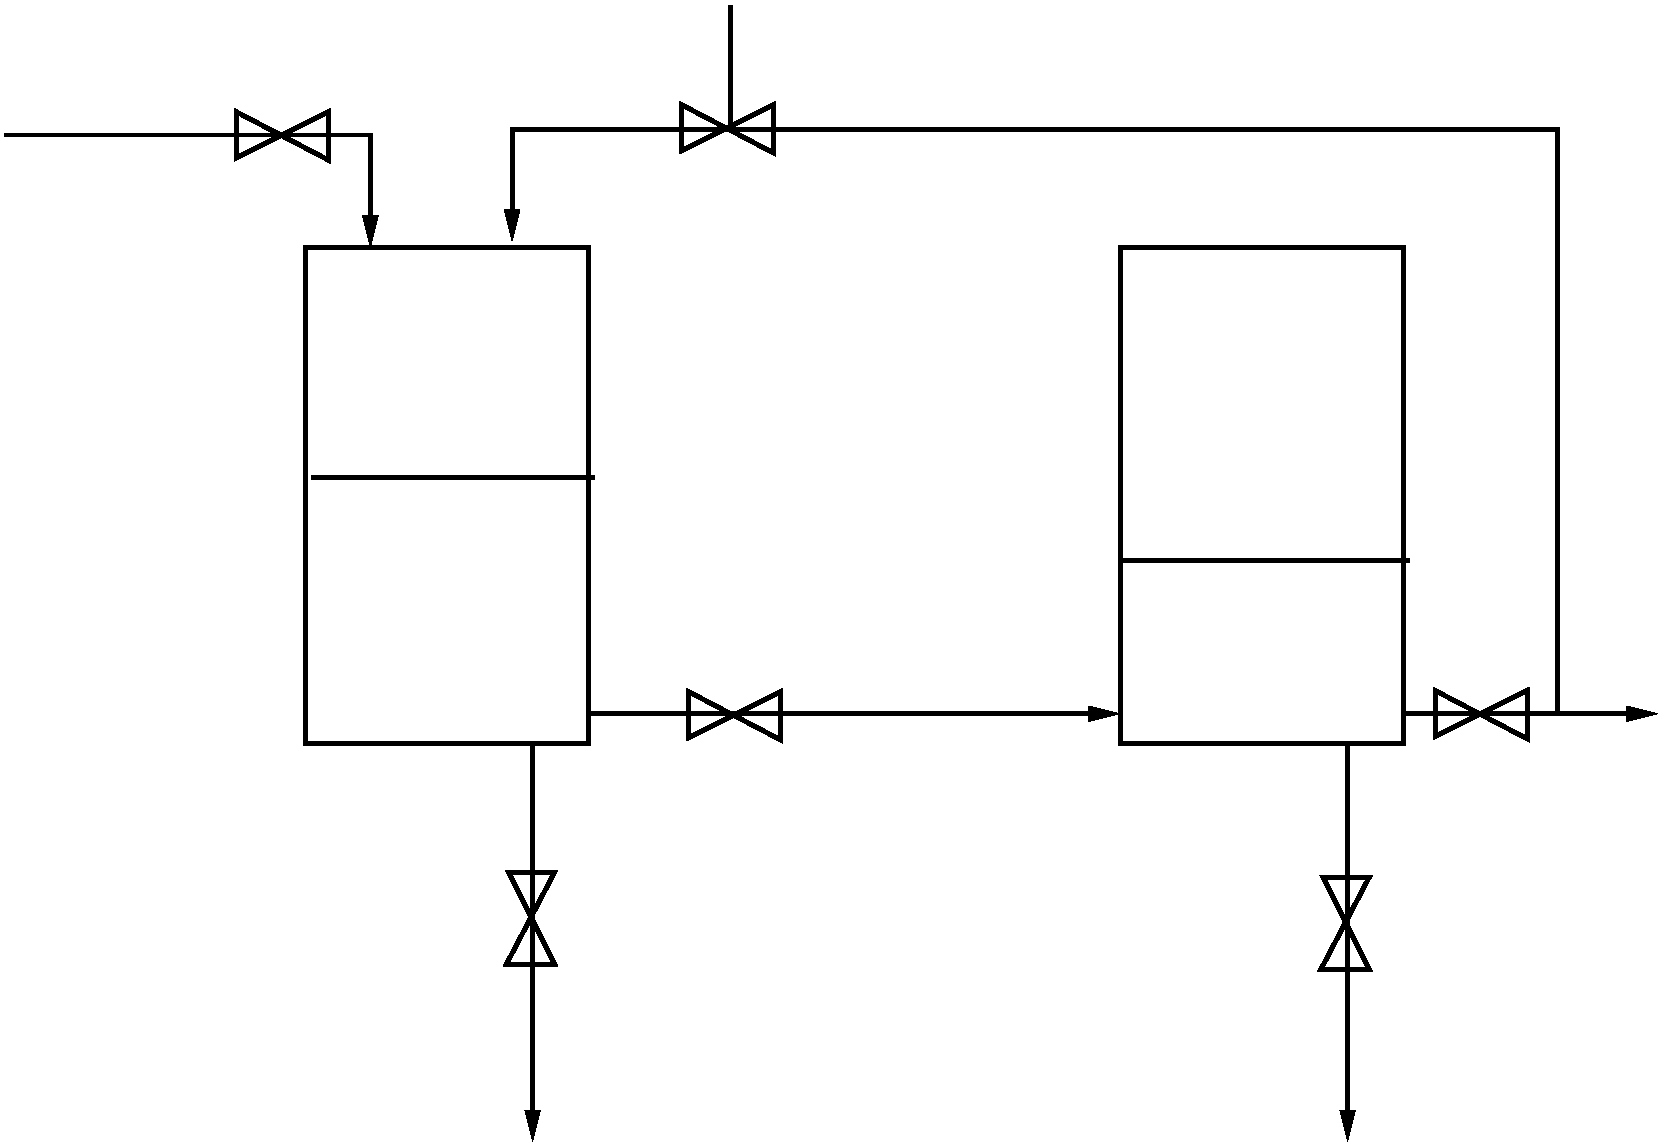
\includegraphics{mpc/2tanks_dist}%
\end{picture}%
\setlength{\unitlength}{4144sp}%
%
\begingroup\makeatletter\ifx\SetFigFont\undefined%
\gdef\SetFigFont#1#2#3#4#5{%
  \reset@font\fontsize{#1}{#2pt}%
  \fontfamily{#3}\fontseries{#4}\fontshape{#5}%
  \selectfont}%
\fi\endgroup%
\begin{picture}(12666,8726)(688,-8079)
\put(11881,-5326){\makebox(0,0)[lb]{\smash{{\SetFigFont{20}{24.0}{\rmdefault}{\mddefault}{\updefault}{\color[rgb]{0,0,0}$u_{21}$}%
}}}}
\put(1216,-646){\makebox(0,0)[lb]{\smash{{\SetFigFont{20}{24.0}{\rmdefault}{\mddefault}{\updefault}{\color[rgb]{0,0,0}$u_{11}$}%
}}}}
\put(4141,-106){\makebox(0,0)[lb]{\smash{{\SetFigFont{20}{24.0}{\rmdefault}{\mddefault}{\updefault}{\color[rgb]{0,0,0}$(1+r) u_{21}$}%
}}}}
\put(7966,-151){\makebox(0,0)[lb]{\smash{{\SetFigFont{20}{24.0}{\rmdefault}{\mddefault}{\updefault}{\color[rgb]{0,0,0}$r u_{21}$}%
}}}}
\put(9991,-4471){\makebox(0,0)[lb]{\smash{{\SetFigFont{20}{24.0}{\rmdefault}{\mddefault}{\updefault}{\color[rgb]{0,0,0}$x_2$}%
}}}}
\put(3871,-4021){\makebox(0,0)[lb]{\smash{{\SetFigFont{20}{24.0}{\rmdefault}{\mddefault}{\updefault}{\color[rgb]{0,0,0}$x_1$}%
}}}}
\put(6886,-5101){\makebox(0,0)[lb]{\smash{{\SetFigFont{20}{24.0}{\rmdefault}{\mddefault}{\updefault}{\color[rgb]{0,0,0}$u_{12}$}%
}}}}
\put(4951,-7846){\makebox(0,0)[lb]{\smash{{\SetFigFont{20}{24.0}{\rmdefault}{\mddefault}{\updefault}{\color[rgb]{0,0,0}$u_{13}$}%
}}}}
\put(11161,-7756){\makebox(0,0)[lb]{\smash{{\SetFigFont{20}{24.0}{\rmdefault}{\mddefault}{\updefault}{\color[rgb]{0,0,0}$u_{22}$}%
}}}}
\end{picture}%
}}
\caption{The two-tank system.}
\label{fig:2tankunstable}
\end{figure}

The subsystem-1 model for the two-tank system is
\begin{equation}
x_1^+ = \underbrace{1}_{A_{1}}x_1 + \underbrace{\begin{bmatrix}1 &-1 
  &-1\end{bmatrix}}_{B_{11}}\underbrace{\begin{bmatrix}u_{11}\\u_{12}\\u_{13}\end{bmatrix}}_{u_1}
+\underbrace{\begin{bmatrix}1+r &0
    \end{bmatrix}}_{B_{12}}\underbrace{\begin{bmatrix}u_{21}\\u_{22}\end{bmatrix}}_{u_2}
%\label{eq:2tanks_subsystem1}
\end{equation}
The subsystem-2 model for the two-tank system is
\begin{equation}
x_2^+ = \underbrace{1}_{A_{2}}x_2 +
\underbrace{\begin{bmatrix}0&1&0\end{bmatrix}}_{B_{21}}\underbrace{\begin{bmatrix}u_{11}\\u_{12}\\u_{13}\end{bmatrix}}_{u_1}
 +\underbrace{\begin{bmatrix}-1&-1\end{bmatrix}}_{B_{22}}\underbrace{\begin{bmatrix}u_{21}\\u_{22}\end{bmatrix}}_{u_2}
%\label{eq:2tanks_subsystem2}
\end{equation}
The overall (centralized) model of the two-tank system is the minimum
realization of
\begin{equation}
x^+ = \underbrace{\begin{bmatrix}A_1 &0\\0& A_2\end{bmatrix}}_{A}x
  + \underbrace{\begin{bmatrix}B_{11}&B_{12}\\B_{21} & B_{22} \end{bmatrix}}_{B} u
%\label{eq:centsystem}
\end{equation}
in which $x = (x_1,x_2)$ and $u =
(u_{11},u_{12},u_{13},u_{21},u_{22})$.
Each input  is constrained to lie between $[0,\bar{u}]$ in which
$0$ corresponds to the valve  completely closed and $\bar{u}$
corresponds to the valve  completely open. The upper bound on the
valve was chosen to be arbitrarily large.

We define stage costs $\ell_1(\cdot,\cdot)$ and $\ell_2(\cdot,\cdot)$:
\begin{align*}
 \ell_1(x_1,u_1)& = x_1^2+u_{11}^2+ u_{12}^2+
100u_{13}^2 \\
\ell_2(x_2,u_2)& = x_2^2+u_{21}^2+ 100u_{22}^2
\end{align*}
 
 The system starts at 
steady state with tank levels $(7,7)$ and all valves closed. At time $t=0$, we change the setpoint of the
two tanks to level $(3,3)$ and all valves closed.

The responses are shown in Figure \ref{fig:mpc:unstable}.
In noncooperative MPC, each subsystem uses the cheap input
$u_{12},u_{21}$ to change the tank levels; unaware that this choice
of inputs leads to instability by introducing more water into the
system. The subsystems manipulate the cheap inputs because the
influence of their inputs on the other subsystem is not captured in
the noncooperative MPC optimization problem.
At each iteration, the two subsystems, optimizing independently, harm each other because they do
not want to operate the expensive valves $u_{13}$ and $u_{22}$.
\begin{figure}
\centering
\scriptsize
\resizebox{\textwidth}{!}{% GNUPLOT: LaTeX picture with Postscript
\begingroup
  \makeatletter
  \providecommand\color[2][]{%
    \GenericError{(gnuplot) \space\space\space\@spaces}{%
      Package color not loaded in conjunction with
      terminal option `colourtext'%
    }{See the gnuplot documentation for explanation.%
    }{Either use 'blacktext' in gnuplot or load the package
      color.sty in LaTeX.}%
    \renewcommand\color[2][]{}%
  }%
  \providecommand\includegraphics[2][]{%
    \GenericError{(gnuplot) \space\space\space\@spaces}{%
      Package graphicx or graphics not loaded%
    }{See the gnuplot documentation for explanation.%
    }{The gnuplot epslatex terminal needs graphicx.sty or graphics.sty.}%
    \renewcommand\includegraphics[2][]{}%
  }%
  \providecommand\rotatebox[2]{#2}%
  \@ifundefined{ifGPcolor}{%
    \newif\ifGPcolor
    \GPcolortrue
  }{}%
  \@ifundefined{ifGPblacktext}{%
    \newif\ifGPblacktext
    \GPblacktexttrue
  }{}%
  % define a \g@addto@macro without @ in the name:
  \let\gplgaddtomacro\g@addto@macro
  % define empty templates for all commands taking text:
  \gdef\gplbacktext{}%
  \gdef\gplfronttext{}%
  \makeatother
  \ifGPblacktext
    % no textcolor at all
    \def\colorrgb#1{}%
    \def\colorgray#1{}%
  \else
    % gray or color?
    \ifGPcolor
      \def\colorrgb#1{\color[rgb]{#1}}%
      \def\colorgray#1{\color[gray]{#1}}%
      \expandafter\def\csname LTw\endcsname{\color{white}}%
      \expandafter\def\csname LTb\endcsname{\color{black}}%
      \expandafter\def\csname LTa\endcsname{\color{black}}%
      \expandafter\def\csname LT0\endcsname{\color[rgb]{1,0,0}}%
      \expandafter\def\csname LT1\endcsname{\color[rgb]{0,1,0}}%
      \expandafter\def\csname LT2\endcsname{\color[rgb]{0,0,1}}%
      \expandafter\def\csname LT3\endcsname{\color[rgb]{1,0,1}}%
      \expandafter\def\csname LT4\endcsname{\color[rgb]{0,1,1}}%
      \expandafter\def\csname LT5\endcsname{\color[rgb]{1,1,0}}%
      \expandafter\def\csname LT6\endcsname{\color[rgb]{0,0,0}}%
      \expandafter\def\csname LT7\endcsname{\color[rgb]{1,0.3,0}}%
      \expandafter\def\csname LT8\endcsname{\color[rgb]{0.5,0.5,0.5}}%
    \else
      % gray
      \def\colorrgb#1{\color{black}}%
      \def\colorgray#1{\color[gray]{#1}}%
      \expandafter\def\csname LTw\endcsname{\color{white}}%
      \expandafter\def\csname LTb\endcsname{\color{black}}%
      \expandafter\def\csname LTa\endcsname{\color{black}}%
      \expandafter\def\csname LT0\endcsname{\color{black}}%
      \expandafter\def\csname LT1\endcsname{\color{black}}%
      \expandafter\def\csname LT2\endcsname{\color{black}}%
      \expandafter\def\csname LT3\endcsname{\color{black}}%
      \expandafter\def\csname LT4\endcsname{\color{black}}%
      \expandafter\def\csname LT5\endcsname{\color{black}}%
      \expandafter\def\csname LT6\endcsname{\color{black}}%
      \expandafter\def\csname LT7\endcsname{\color{black}}%
      \expandafter\def\csname LT8\endcsname{\color{black}}%
    \fi
  \fi
  \setlength{\unitlength}{0.0500bp}%
  \begin{picture}(7200.00,2520.00)%
    \gplgaddtomacro\gplbacktext{%
      \csname LTb\endcsname%
      \put(814,440){\makebox(0,0)[r]{\strut{} 0}}%
      \put(814,1348){\makebox(0,0)[r]{\strut{} 5}}%
      \put(814,2256){\makebox(0,0)[r]{\strut{} 10}}%
      \put(946,220){\makebox(0,0){\strut{} 0}}%
      \put(1758,220){\makebox(0,0){\strut{} 10}}%
      \put(2571,220){\makebox(0,0){\strut{} 20}}%
      \put(3383,220){\makebox(0,0){\strut{} 30}}%
      \put(176,1348){\rotatebox{-270}{\makebox(0,0){\strut{}Level -1}}}%
    }%
    \gplgaddtomacro\gplfronttext{%
      \csname LTb\endcsname%
      \put(1541,875){\makebox(0,0)[r]{\strut{}ncoop}}%
      \csname LTb\endcsname%
      \put(1541,655){\makebox(0,0)[r]{\strut{}coop}}%
      \csname LTb\endcsname%
      \put(2792,875){\makebox(0,0)[r]{\strut{}cent}}%
    }%
    \gplgaddtomacro\gplbacktext{%
      \csname LTb\endcsname%
      \put(4109,220){\makebox(0,0){\strut{} 0}}%
      \put(4833,220){\makebox(0,0){\strut{} 10}}%
      \put(5558,220){\makebox(0,0){\strut{} 20}}%
      \put(6282,220){\makebox(0,0){\strut{} 30}}%
      \put(6414,440){\makebox(0,0)[l]{\strut{} 0}}%
      \put(6414,1348){\makebox(0,0)[l]{\strut{} 5}}%
      \put(6414,2256){\makebox(0,0)[l]{\strut{} 10}}%
      \put(7051,1348){\rotatebox{-270}{\makebox(0,0){\strut{}Level-2}}}%
    }%
    \gplgaddtomacro\gplfronttext{%
    }%
    \gplbacktext
    \put(0,0){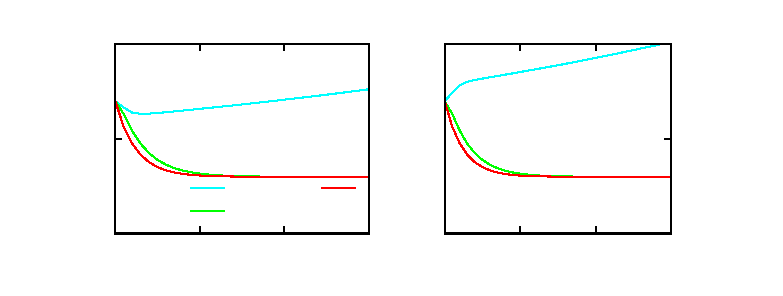
\includegraphics{mpc/unstable_x}}%
    \gplfronttext
  \end{picture}%
\endgroup
}
\resizebox{\textwidth}{!}{% GNUPLOT: LaTeX picture with Postscript
\begingroup
  \makeatletter
  \providecommand\color[2][]{%
    \GenericError{(gnuplot) \space\space\space\@spaces}{%
      Package color not loaded in conjunction with
      terminal option `colourtext'%
    }{See the gnuplot documentation for explanation.%
    }{Either use 'blacktext' in gnuplot or load the package
      color.sty in LaTeX.}%
    \renewcommand\color[2][]{}%
  }%
  \providecommand\includegraphics[2][]{%
    \GenericError{(gnuplot) \space\space\space\@spaces}{%
      Package graphicx or graphics not loaded%
    }{See the gnuplot documentation for explanation.%
    }{The gnuplot epslatex terminal needs graphicx.sty or graphics.sty.}%
    \renewcommand\includegraphics[2][]{}%
  }%
  \providecommand\rotatebox[2]{#2}%
  \@ifundefined{ifGPcolor}{%
    \newif\ifGPcolor
    \GPcolortrue
  }{}%
  \@ifundefined{ifGPblacktext}{%
    \newif\ifGPblacktext
    \GPblacktexttrue
  }{}%
  % define a \g@addto@macro without @ in the name:
  \let\gplgaddtomacro\g@addto@macro
  % define empty templates for all commands taking text:
  \gdef\gplbacktext{}%
  \gdef\gplfronttext{}%
  \makeatother
  \ifGPblacktext
    % no textcolor at all
    \def\colorrgb#1{}%
    \def\colorgray#1{}%
  \else
    % gray or color?
    \ifGPcolor
      \def\colorrgb#1{\color[rgb]{#1}}%
      \def\colorgray#1{\color[gray]{#1}}%
      \expandafter\def\csname LTw\endcsname{\color{white}}%
      \expandafter\def\csname LTb\endcsname{\color{black}}%
      \expandafter\def\csname LTa\endcsname{\color{black}}%
      \expandafter\def\csname LT0\endcsname{\color[rgb]{1,0,0}}%
      \expandafter\def\csname LT1\endcsname{\color[rgb]{0,1,0}}%
      \expandafter\def\csname LT2\endcsname{\color[rgb]{0,0,1}}%
      \expandafter\def\csname LT3\endcsname{\color[rgb]{1,0,1}}%
      \expandafter\def\csname LT4\endcsname{\color[rgb]{0,1,1}}%
      \expandafter\def\csname LT5\endcsname{\color[rgb]{1,1,0}}%
      \expandafter\def\csname LT6\endcsname{\color[rgb]{0,0,0}}%
      \expandafter\def\csname LT7\endcsname{\color[rgb]{1,0.3,0}}%
      \expandafter\def\csname LT8\endcsname{\color[rgb]{0.5,0.5,0.5}}%
    \else
      % gray
      \def\colorrgb#1{\color{black}}%
      \def\colorgray#1{\color[gray]{#1}}%
      \expandafter\def\csname LTw\endcsname{\color{white}}%
      \expandafter\def\csname LTb\endcsname{\color{black}}%
      \expandafter\def\csname LTa\endcsname{\color{black}}%
      \expandafter\def\csname LT0\endcsname{\color{black}}%
      \expandafter\def\csname LT1\endcsname{\color{black}}%
      \expandafter\def\csname LT2\endcsname{\color{black}}%
      \expandafter\def\csname LT3\endcsname{\color{black}}%
      \expandafter\def\csname LT4\endcsname{\color{black}}%
      \expandafter\def\csname LT5\endcsname{\color{black}}%
      \expandafter\def\csname LT6\endcsname{\color{black}}%
      \expandafter\def\csname LT7\endcsname{\color{black}}%
      \expandafter\def\csname LT8\endcsname{\color{black}}%
    \fi
  \fi
  \setlength{\unitlength}{0.0500bp}%
  \begin{picture}(7200.00,2520.00)%
    \gplgaddtomacro\gplbacktext{%
      \csname LTb\endcsname%
      \put(682,803){\makebox(0,0)[r]{\strut{} 0}}%
      \put(682,2256){\makebox(0,0)[r]{\strut{} 2}}%
      \put(814,220){\makebox(0,0){\strut{} 0}}%
      \put(1670,220){\makebox(0,0){\strut{} 10}}%
      \put(2527,220){\makebox(0,0){\strut{} 20}}%
      \put(3383,220){\makebox(0,0){\strut{} 30}}%
      \put(176,1348){\rotatebox{-270}{\makebox(0,0){\strut{}Tank-1 Cheap input}}}%
    }%
    \gplgaddtomacro\gplfronttext{%
    }%
    \gplgaddtomacro\gplbacktext{%
      \csname LTb\endcsname%
      \put(4109,220){\makebox(0,0){\strut{} 0}}%
      \put(4877,220){\makebox(0,0){\strut{} 10}}%
      \put(5646,220){\makebox(0,0){\strut{} 20}}%
      \put(6414,220){\makebox(0,0){\strut{} 30}}%
      \put(6546,803){\makebox(0,0)[l]{\strut{} 0}}%
      \put(6546,1530){\makebox(0,0)[l]{\strut{} 1}}%
      \put(6546,2256){\makebox(0,0)[l]{\strut{} 2}}%
      \put(7051,1348){\rotatebox{-270}{\makebox(0,0){\strut{}Tank-1 Expensive input}}}%
    }%
    \gplgaddtomacro\gplfronttext{%
    }%
    \gplbacktext
    \put(0,0){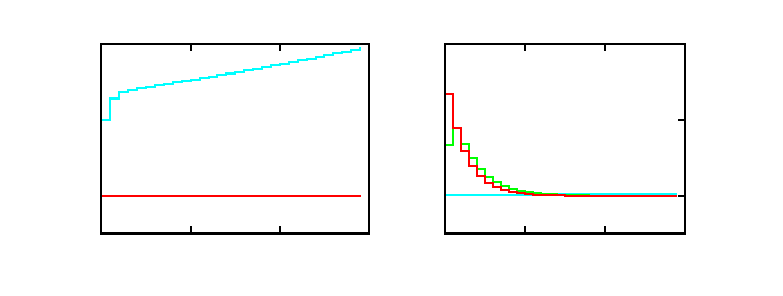
\includegraphics{mpc/unstable_u1}}%
    \gplfronttext
  \end{picture}%
\endgroup
}
\resizebox{\textwidth}{!}{% GNUPLOT: LaTeX picture with Postscript
\begingroup
  \makeatletter
  \providecommand\color[2][]{%
    \GenericError{(gnuplot) \space\space\space\@spaces}{%
      Package color not loaded in conjunction with
      terminal option `colourtext'%
    }{See the gnuplot documentation for explanation.%
    }{Either use 'blacktext' in gnuplot or load the package
      color.sty in LaTeX.}%
    \renewcommand\color[2][]{}%
  }%
  \providecommand\includegraphics[2][]{%
    \GenericError{(gnuplot) \space\space\space\@spaces}{%
      Package graphicx or graphics not loaded%
    }{See the gnuplot documentation for explanation.%
    }{The gnuplot epslatex terminal needs graphicx.sty or graphics.sty.}%
    \renewcommand\includegraphics[2][]{}%
  }%
  \providecommand\rotatebox[2]{#2}%
  \@ifundefined{ifGPcolor}{%
    \newif\ifGPcolor
    \GPcolortrue
  }{}%
  \@ifundefined{ifGPblacktext}{%
    \newif\ifGPblacktext
    \GPblacktexttrue
  }{}%
  % define a \g@addto@macro without @ in the name:
  \let\gplgaddtomacro\g@addto@macro
  % define empty templates for all commands taking text:
  \gdef\gplbacktext{}%
  \gdef\gplfronttext{}%
  \makeatother
  \ifGPblacktext
    % no textcolor at all
    \def\colorrgb#1{}%
    \def\colorgray#1{}%
  \else
    % gray or color?
    \ifGPcolor
      \def\colorrgb#1{\color[rgb]{#1}}%
      \def\colorgray#1{\color[gray]{#1}}%
      \expandafter\def\csname LTw\endcsname{\color{white}}%
      \expandafter\def\csname LTb\endcsname{\color{black}}%
      \expandafter\def\csname LTa\endcsname{\color{black}}%
      \expandafter\def\csname LT0\endcsname{\color[rgb]{1,0,0}}%
      \expandafter\def\csname LT1\endcsname{\color[rgb]{0,1,0}}%
      \expandafter\def\csname LT2\endcsname{\color[rgb]{0,0,1}}%
      \expandafter\def\csname LT3\endcsname{\color[rgb]{1,0,1}}%
      \expandafter\def\csname LT4\endcsname{\color[rgb]{0,1,1}}%
      \expandafter\def\csname LT5\endcsname{\color[rgb]{1,1,0}}%
      \expandafter\def\csname LT6\endcsname{\color[rgb]{0,0,0}}%
      \expandafter\def\csname LT7\endcsname{\color[rgb]{1,0.3,0}}%
      \expandafter\def\csname LT8\endcsname{\color[rgb]{0.5,0.5,0.5}}%
    \else
      % gray
      \def\colorrgb#1{\color{black}}%
      \def\colorgray#1{\color[gray]{#1}}%
      \expandafter\def\csname LTw\endcsname{\color{white}}%
      \expandafter\def\csname LTb\endcsname{\color{black}}%
      \expandafter\def\csname LTa\endcsname{\color{black}}%
      \expandafter\def\csname LT0\endcsname{\color{black}}%
      \expandafter\def\csname LT1\endcsname{\color{black}}%
      \expandafter\def\csname LT2\endcsname{\color{black}}%
      \expandafter\def\csname LT3\endcsname{\color{black}}%
      \expandafter\def\csname LT4\endcsname{\color{black}}%
      \expandafter\def\csname LT5\endcsname{\color{black}}%
      \expandafter\def\csname LT6\endcsname{\color{black}}%
      \expandafter\def\csname LT7\endcsname{\color{black}}%
      \expandafter\def\csname LT8\endcsname{\color{black}}%
    \fi
  \fi
  \setlength{\unitlength}{0.0500bp}%
  \begin{picture}(7200.00,2520.00)%
    \gplgaddtomacro\gplbacktext{%
      \csname LTb\endcsname%
      \put(682,1014){\makebox(0,0)[r]{\strut{} 0}}%
      \put(682,2256){\makebox(0,0)[r]{\strut{} 2}}%
      \put(814,484){\makebox(0,0){\strut{} 0}}%
      \put(1670,484){\makebox(0,0){\strut{} 10}}%
      \put(2527,484){\makebox(0,0){\strut{} 20}}%
      \put(3383,484){\makebox(0,0){\strut{} 30}}%
      \put(176,1480){\rotatebox{-270}{\makebox(0,0){\strut{}Tank-2 Cheap valve}}}%
      \put(2098,154){\makebox(0,0){\strut{}Time}}%
    }%
    \gplgaddtomacro\gplfronttext{%
    }%
    \gplgaddtomacro\gplbacktext{%
      \csname LTb\endcsname%
      \put(4109,484){\makebox(0,0){\strut{} 0}}%
      \put(4877,484){\makebox(0,0){\strut{} 10}}%
      \put(5646,484){\makebox(0,0){\strut{} 20}}%
      \put(6414,484){\makebox(0,0){\strut{} 30}}%
      \put(6546,1014){\makebox(0,0)[l]{\strut{} 0}}%
      \put(6546,1635){\makebox(0,0)[l]{\strut{} 1}}%
      \put(6546,2256){\makebox(0,0)[l]{\strut{} 2}}%
      \put(7051,1480){\rotatebox{-270}{\makebox(0,0){\strut{}Tank-2 Expensive valve}}}%
      \put(5261,154){\makebox(0,0){\strut{}Time}}%
    }%
    \gplgaddtomacro\gplfronttext{%
    }%
    \gplbacktext
    \put(0,0){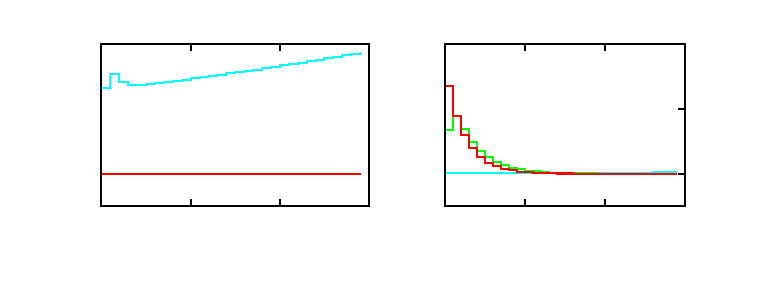
\includegraphics{mpc/unstable_u2}}%
    \gplfronttext
  \end{picture}%
\endgroup
}
\caption{State and input profiles for two-tank system under
  distributed MPC (ncoop: noncooperative, coop: cooperative, cent: centralized).}
\label{fig:mpc:unstable}
\end{figure}
In cooperative MPC, subsystem-2 realizes that operating valve $u_{21}$
is not desirable, because it optimizes the overall objective function. The subsystems now judiciously use the expensive
valves to maintain stability.



\section{Robust cooperative MPC}
\label{sec:mpc:robust}
\subsection{Preliminaries}
We consider the centralized system \eqref{eq:mpc:distributed:cent}
obtained from the distributed models \eqref{eq:mpc:distributed:dynamics},  subject to bounded additive
disturbance as follows:
\begin{equation}
\label{eq:mpc:model_dist}
x^+ = Ax + Bu + w
\end{equation}
in which the inputs are assumed to lie in set $u_i \in \mathbb{U}_i$
as in the previous section. The assumptions on the disturbance are
stated in Assumption \ref{ass:mpc:W}

\begin{assumption}[Bounded disturbance]
\label{ass:mpc:W}
The additive disturbance $w$ lies in a convex, closed and, compact set $\mathbb{W}$
containing the origin in its interior.
\end{assumption}

The nominal system, without the additive disturbance is denoted as
follows, using $z,v$ for the nominal state and input variables.

\begin{equation}
\label{eq:mpc:model_nominal}
z^+ = Az + Bv
\end{equation}

At any time $k$, we can write the deviation between the actual state
and the nominal state as $e(k) = x(k)-z(k)$. If the inputs to both the
nominal and actual system were the same, then the error dynamics can
be written as:

\begin{equation}
\label{eq:mpc:error_dynamics}
e^+ = Ax+Bu+w - Az+Bu = Ae + w
\end{equation}

Hence, given an initial $e(0)=0$, the error at time $k$ lies in the
following set:

\begin{equation}
\label{eq:mpc:error_set}
e(k) \in S(k) :=\sum_{j=0}^{k-1}A^j\mathbb{W} = \mathbb{W} \oplus A\mathbb{W}
\oplus \ldots \oplus A^{k-1}\mathbb{W}
\end{equation}
in which $A^j\mathbb{W}$ indicates set multiplication. That is,

\[A^j\mathbb{W} := \set{A^jw \mid \forall w \in \mathbb{W}}
\]

The symbol $\oplus$ indicates set addition. That is,
\[ \mathbb{W} \oplus A\mathbb{W} := \set{w_1+w_2 \mid w_1 \in
  \mathbb{W}, w_2 \in A\mathbb{W}}\]

For stable $A$, it can be shown that the set $S(\infty)$ exists and is
positive invariant for the system \eqref{eq:mpc:error_dynamics}
\citep{kolmanovsky:gilbert:1998}.


\subsection{Tube based MPC}

We now discuss tube based MPC \citep[Chapter 3]{rawlings:mayne:2009}, the basic idea for which is as follows: (i)
use MPC on the nominal system to find $v(k) = \kappa(z(k))$,  and (ii)
based on the error at time $k$, $e(k)$, find the input to the plant as $u(k) = v(k) + Ke(k)$

By design, we select a $K$ such that $A_K:=A+BK$ is Hurwitz. Such a choice
implies that the error dynamics in the closed-loop is:
\begin{equation}
\label{eq:mpc:error_CL}
e^+ = x^+-z^+=Ax+Bv+BK(x-z)+w-Az-Bv = A_Ke+w
\end{equation}

Now, since $A_K$ is stable, we can conclude that $S_K(\infty) =
\sum_{j=0}^{\infty}A_K^j\mathbb{W}$ exists and is positive invariant
for \eqref{eq:mpc:error_CL}.

The stability and convergence theorems are therefore based on the
following observations:(i) the origin is asymptotically stable for the
nominal system $z^+= Az+B\kappa(z)$ by design, (ii) the error is designed to lie in the set
$S_K(\infty)$ by the   choice of $K$ and input $u = \kappa(z) +
K(x-z)$, and (iii) the actual state $x(k); k \rightarrow \infty$
therefore belongs to the set   $\set{0} \times S_K(\infty)$

In the presence of persistent disturbance, we ensure that the states
lie inside a bounded set that we can compute offline. The name tube
based MPC comes from the fact that at each time $k$, the state $x$
lies in a ``tube'' defined by $x(k) \in z(k)\oplus S_K(\infty)$
.  

For the inputs $u = v+K(x-z)$ to remain feasible, we need to ensure
that $v$ satisfies the tighter constraints\footnote{If state constraints are present, they need to be tightened
  as well. We do not discuss state constraints because of Assumption \ref{ass:mpc:noX}.}:
\begin{equation}
\mathbb{V} := \mathbb{U} \ominus KS_K(\infty)
\end{equation}
The tighter set follows from the fact that $e = (x-z) \in
S_K(\infty)$. 

The nominal MPC problem is defined as:
\begin{align}
\tilde{\mathbb{P}}_N(z): & \min_{\mathbf{v}}V_N(z,\mathbf{v}) \nonumber \\
& \text{s.t.~} z(j+1) = Az(j) + Bv(j)&  j = \set{0,1,\ldots,N-1}\nonumber\\
& v(j) \in \mathbb{V} \label{eq:mpc:robust:PNz},
& \qquad   j = \set{0,1,\ldots,N-1}\\
&z(0) = z \nonumber \\
& z(N) \in \mathbb{Z}_f \nonumber
\end{align}
in which $\mathbb{Z}_f$ is a terminal set that satisfies Assumption
\ref{ass:mpc:bsa} and $V_N(z,\mathbf{v})$ is the cost function defined by
\eqref{eq:mpc:VN}. Let $\kappa_s(z)$ denote the input law obtained by
implementing a suboptimal MPC algorithm on \eqref{eq:mpc:robust:PNz}. Then the
origin is asymptotically stable for the closed loop $z^+ = Az+
B\kappa_s(z)$ by Theorem \ref{thm:mpc:suboptimal}. Now, if input $u =
\kappa_s(z) + K(x-z)$ is injected to the plant, then $e \in
S_K(\infty)$. Hence, we can prove that $\mathcal{A}: = \set{0} \times
S_K(\infty)$ is asymptotically stable for the composite system 
\begin{align}
z^+ &= Az + B\kappa_s(z)\\
x^+ &= Ax + B\kappa_s(z) + BK(x-z) + w 
\end{align}

The region of attraction is $\mathcal{Z}_N \times \mathcal{X}_N$, in
which $\mathcal{Z}_N$ is the following projection:
\[ \mathcal{Z}_N : = \set{z \mid \mathbf{v} \in \mathbb{V}^N \text{s.t.~}
  z(N;z,\mathbf{v}) \in \mathbb{Z}_f}\]
and $\mathcal{X}_N := \mathcal{Z}_N \oplus S_K(\infty)$.

\subsection{Main results}
Recall that if we use the relaxation formulation to remove the
terminal region constraints in cooperative MPC, then each-time the
warm start becomes infeasible, we need a warm start recovery step,
which is the following projection onto convex sets problem:
\[ \set{\tilde{\bu}(x) \mid V_N^\beta(x,\tilde{\bu})\leq \bar{V}, \tilde{\bu}_i \in
  \mathbb{U}_i \forall i \in \set{1,2,\ldots,M}}\]
Distributed algorithms for projection onto convex sets or the convex
feasibility problems recover feasibility only at convergence. Hence,
such algorithms are not suitable for distributed warm-start
re-initialization since we cannot guarantee convergence within the
sampling time. 

To overcome these problems, we propose tube based robust cooperative
MPC that is based on two important observations:(i)  the optimization problems in tube based MPC are based on the
  nominal system, and (ii) by design, the warm start is feasible for $z^+$ if the input $v
  = \mathbf{v}(0;z)$ is implemented for the nominal system. Hence, we
  can conclude that the warm start based on the nominal MPC, $\tilde{\mathbf{v}}$, always remains feasible for the nominal problem. Furthermore, as we
discussed in Section \ref{sec:mpc:distributed:coop}, cooperative MPC stabilizes
the nominal system. Hence, we can use cooperative MPC for the nominal
system. The only caveat is that to ensure convergence to the
centralized solution, we need to have that the input sets are
uncoupled. In this case, if we wish to implement cooperative MPC on
the nominal system, we need to have that the set $\mathbb{V}$ be
uncoupled, that is 
\[ \mathbb{V} = \mathbb{V}_1 \times \mathbb{V}_2 \times \ldots \times
\mathbb{V}_M \]

In tube based MPC, the tightened set $\mathbb{V}$ is dependent
on $K$, $S_K(\infty)$ and the original disturbance set $\mathbb{W}$. So,
there is no guarantee that $\mathbb{V}$ does not have coupling between
the inputs. Therefore, we introduce another offline calculation, which
is to find a hyperbox $\tilde{\mathbb{V}}$ that lies completely inside $\mathbb{V}$. 

\begin{remark}
As shown in \citet{rakovic:kerrigan:kouramas:mayne:2003}, it is not necessary to
calculate $S_K(\infty)$ to obtain approximations to $\mathbb{V}$. In
fact, if the input constraints are polytopic and decoupled, then the
procedure mentioned in
\citet{rakovic:kerrigan:kouramas:mayne:2003}, can be used to obtain
tightened constraints that  are also polytopic and decoupled.
\end{remark} 

As noted earlier, in robust MPC, the optimizations are performed based
on the nominal state information, while the actual state could have
drifted far from the nominal state because of the disturbances. We
therefore use the modified version of the robust MPC algorithm
presented in \citet[P.234]{rawlings:mayne:2009}. 

We choose $\bar{V}, a, \beta$ such that the set 
\[\mathbb{Z}_f := \set{z \mid V_f(z) \leq a} \]
satisfies Assumption \ref{ass:mpc:bsa}. We choose $\bar{V} \geq a$ and
$\beta$ according to Proposition
\ref{prop:mpc:distributed:relaxation:betabar}. The controller gain $K$
is chosen such that the centralized system $(A+BK)$ is stable and the input constraint
set is tightened as:
\[ \tilde{\mathbb{V}} := \tilde{\mathbb{V}}_1 \times
\tilde{\mathbb{V}}_2 \times \ldots \tilde{\mathbb{V}}_M \subseteq
\mathbb{V} := \mathbb{U} \ominus KS_K(\infty) \]


The centralized nominal MPC optimization problem is: 
\begin{align}
\tilde{\mathbb{P}}_N(z): & \min_{\mathbf{v}}V^\beta_N(x,\mathbf{v}) \nonumber \\
& \text{s.t.~} z(j+1) = Az(j) + Bv(j)&   j  =  \set{0,1,\ldots,N-1}\nonumber\\
& v(j) \in \tilde{\mathbb{V}}&  j \set{\in 0,1,\ldots,N-1}  \label{eq:mpc:PNzbeta} \\
& z(0) = z \nonumber
\end{align}
Note that the region of attraction for the cooperative nominal MPC is:
\[ \mathcal{Z}_N : = \set{z \mid \mathbf{v} \in \tilde{\mathbb{V}} \text{s.t.~}
 V_N^\beta(z,\mathbf{v}) \leq \bar{V}}\]

The robust cooperative MPC algorithm is presented in Algorithm \ref{alg:mpc:robust}.
%\begin{algo}[Robust cooperative MPC] \mbox{ }
\begin{algorithm}
 \KwData{Starting state $x(0)$, initial guess
   $(\tilde{\bu}_1(0),\tilde{\bu}_2(0),\ldots,\tilde{\bu}_M(0))$ so
   that $V_N^\beta(x,\tilde{\bu}) \leq \bar{V}$
   $\bar{p} \geq 1$ and $\omega_i \in (0,1)$ such that
   $\sum_{i=0}^{M}\omega_i = 1$}
 \KwResult{Asymptotically stable closed loop}
 {\KwSty{Offline:}} Perform the following computations and share with
 every subsystem
 \Begin{
  Compute $K$ so that $A+BK$ is stable\\
  Compute/ Approximate  $S_K(\infty)$, $\mathbb{V} = \mathbb{U} \ominus KS_K(\infty)$\\
  %Compute/ Approximate $\mathbb{V} = \mathbb{U} \ominus KS_K(\infty)$\\
  Compute $\tilde{\mathbb{V}}_i$ so that $\tilde{\mathbb{V}}_1 \times
  \tilde{\mathbb{V}}_2 \times \ldots \times \tilde{\mathbb{V}}_M 
  \subseteq \mathbb{V}$\\
 }
{\KwSty{Online:}}
\Begin{
 set $z(0) \leftarrow x(0); \tilde{\mathbf{v}}(0) \leftarrow \tilde{\bu}(0)$\\
 set $k \leftarrow 0$\\
 \While {$k \geq 0$}{
   Set $p \leftarrow 0$\\
   Set $\mathbf{v}_i^{(p)} \leftarrow \tilde{\mathbf{v}}_i(k)$ for $i = 1,2,\ldots,M$\\
   Broadcast current subsystem inputs $\tilde{\mathbf{v}}_i(k)$ to other
   subsystems\\
   \While {$p < \bar{p}$}{
       \If {$V_N^\beta(x(k),\tilde{\mathbf{v}}) \leq
         V_N^\beta(z(k),\tilde{\mathbf{v}})\leq \bar{V}$}{
         \KwSty{Reset} $z(k) \leftarrow x(k)$\\
         }
         Solve $\min_{\mathbf{v}_i}V_N^\beta(z,\mathbf{v}) \text{s.t.~}
         \mathbf{v}_i \in \tilde{\mathbb{V}}_i, \mathbf{v}_{-i} =
         \mathbf{v}_{-i}^{(p)}$ to obtain $\mathbf{v}_i^0$ for i in $1,2,\ldots,M$.
         Set $\mathbf{v}_i^{(p+1)} \leftarrow \omega_i \mathbf{v}_i^{(p)} +
         (1-\omega_i) \mathbf{v}_i^0$ for i in $1,2,\ldots,M$ \\
      }
  Set $\mathbf{v} \leftarrow (\mathbf{v}_1^{(p)},\mathbf{v}_2^{(p)},\ldots,\mathbf{v}_M^{(p)})$ and find $z(k+N) \leftarrow
  \phi(N;z(k),\mathbf{v})$\\
  Obtain $v_+ = (v_{1+},v_{2+},\ldots,v_{M+}) \leftarrow \kappa_f(z(k+N))$\\
  Obtain warm start $\tilde{\mathbf{v}}_i(k+1) =
    (\mathbf{v}_i^{(p)}(1),\mathbf{v}_i^{(p)}(2),\ldots,v_{i+})$ for $i = 1,2,\ldots,M$.\\
   Set input as $v(k) =
  (\mathbf{v}_1^{(p)}(0),\mathbf{v}_2^{(p)}(0),\ldots,\mathbf{v}_M^{(p)}(0))$\\
  Evolve nominal state from $z(k)$ to $z(k+1)$ under input $v(k)$\\
  Set input $u(k) = v(k)+ K(x(k) - z(k))$\\
  Evolve state from $x(k)$ to $x(k+1)$ under input $u(k)$\\
 }
}
\caption{Robust cooperative MPC}
\label{alg:mpc:robust}
\end{algorithm}

The modification that we alluded to earlier is the ``if condition'' in
Algorithm \ref{alg:mpc:robust}. The condition states that if the warm start
is feasible for the actual state at time $k$ and satisfies a cost-drop
criteria, then we reset the error to zero. In this way, not only do we not
lose the convergence property of the closed-loop nominal state (since
the cost-drop is satisfied all the time), but we also incorporate
feedback into the system. Another modification to Algorithm
\ref{alg:mpc:robust} is a slow time scale reset of the nominal state to the
actual state. That is, after every $T$ sampling times, in which $T$ is
much larger than the sampling time employed, we automatically reset
the nominal trajectory. However, in this case, we need to ensure that
the warm-start is feasible for the reset. 

\subsection{Example}
Consider the two tank system as shown in Figure
\ref{fig:mpc:two_tanks}. The overall system consists of two tanks which
are the two subsystems. The first subsystem (tank-1) manipulates inputs
$u_1 = (u_{11},u_{12})$, while the second subsystem (tank-2) manipulates
inputs $u_2 = (u_{22})$. There are two disturbances affecting the
system, $w_1$ in the first tank and $w_2$ in the second tank. The
state dynamics for this two tank system is given by:
\begin{equation*}
\begin{bmatrix}x_1\\x_2\end{bmatrix}^+ = \begin{bmatrix}1&\\ &
  1\end{bmatrix} \begin{bmatrix}x_1\\x_2\end{bmatrix}+
\begin{bmatrix} 1 & - 1 \\ 0&
  1 \end{bmatrix}u_1+ \begin{bmatrix}0\\-1\end{bmatrix}u_2
+ \begin{bmatrix}w_1\\w_2\end{bmatrix}
\end{equation*}

\begin{figure*}
\centering
\scriptsize
\resizebox{0.75\textwidth}{!}{\begin{picture}(0,0)%
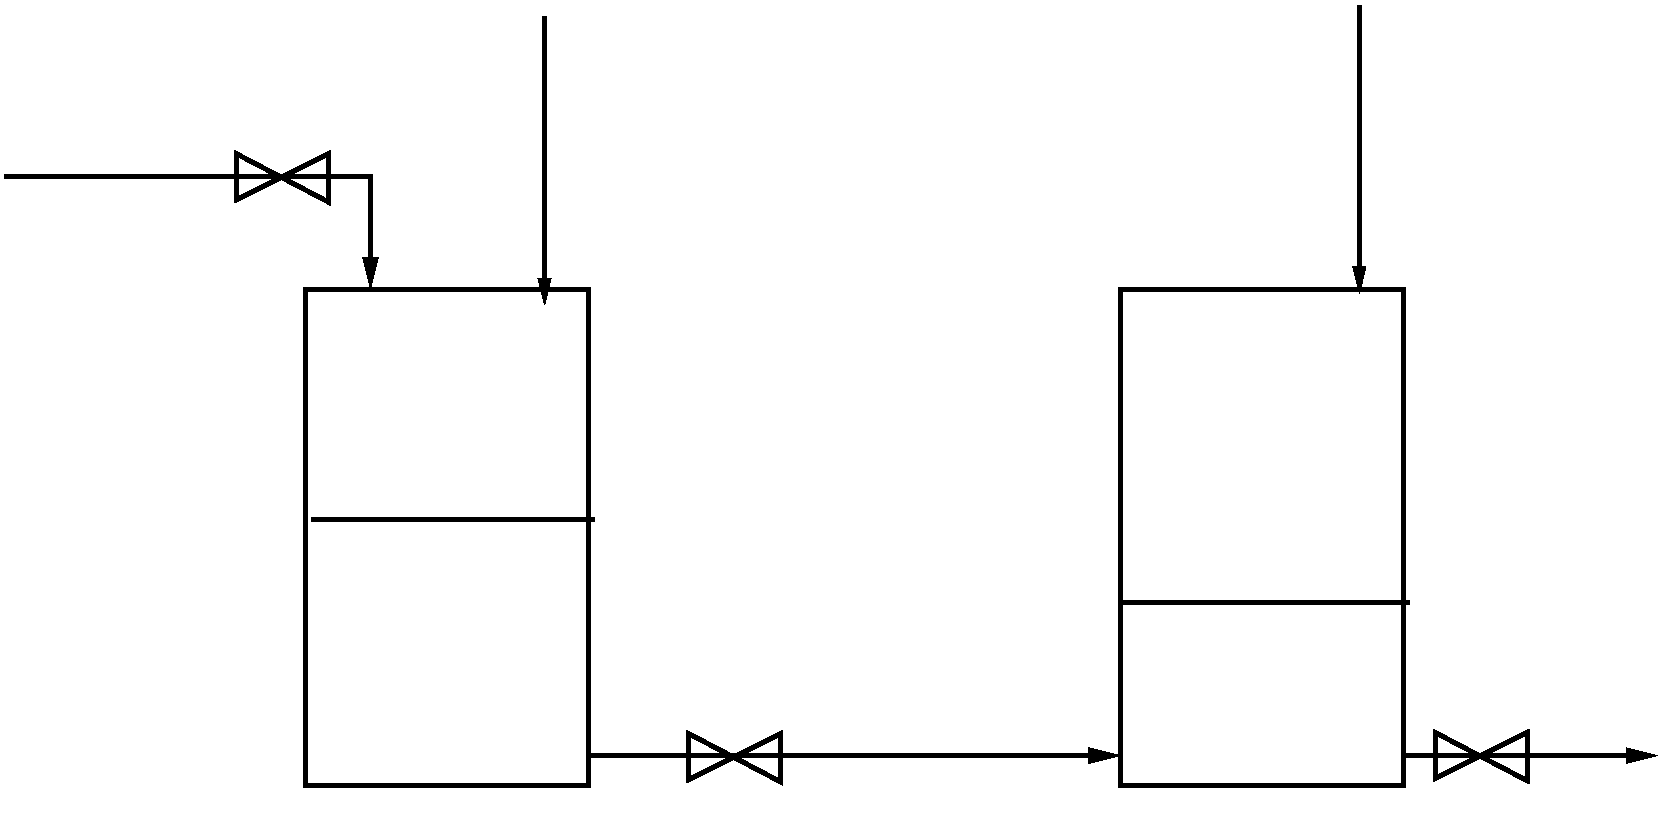
\includegraphics{mpc/two_tanks}%
\end{picture}%
\setlength{\unitlength}{4144sp}%
%
\begingroup\makeatletter\ifx\SetFigFont\undefined%
\gdef\SetFigFont#1#2#3#4#5{%
  \reset@font\fontsize{#1}{#2pt}%
  \fontfamily{#3}\fontseries{#4}\fontshape{#5}%
  \selectfont}%
\fi\endgroup%
\begin{picture}(12666,6356)(688,-5390)
\put(11881,-5326){\makebox(0,0)[lb]{\smash{{\SetFigFont{20}{24.0}{\rmdefault}{\mddefault}{\updefault}{\color[rgb]{0,0,0}$u_{22}$}%
}}}}
\put(1216,-646){\makebox(0,0)[lb]{\smash{{\SetFigFont{20}{24.0}{\rmdefault}{\mddefault}{\updefault}{\color[rgb]{0,0,0}$u_{11}$}%
}}}}
\put(9991,-4471){\makebox(0,0)[lb]{\smash{{\SetFigFont{20}{24.0}{\rmdefault}{\mddefault}{\updefault}{\color[rgb]{0,0,0}$x_2$}%
}}}}
\put(3871,-4021){\makebox(0,0)[lb]{\smash{{\SetFigFont{20}{24.0}{\rmdefault}{\mddefault}{\updefault}{\color[rgb]{0,0,0}$x_1$}%
}}}}
\put(6886,-5101){\makebox(0,0)[lb]{\smash{{\SetFigFont{20}{24.0}{\rmdefault}{\mddefault}{\updefault}{\color[rgb]{0,0,0}$u_{12}$}%
}}}}
\put(5041,-1006){\makebox(0,0)[lb]{\smash{{\SetFigFont{20}{24.0}{\rmdefault}{\mddefault}{\updefault}{\color[rgb]{0,0,0}$w_1$}%
}}}}
\put(11251,-1096){\makebox(0,0)[lb]{\smash{{\SetFigFont{20}{24.0}{\rmdefault}{\mddefault}{\updefault}{\color[rgb]{0,0,0}$w_2$}%
}}}}
\end{picture}%
}
\caption{Two tank system}
\label{fig:mpc:two_tanks}
\end{figure*}

We assume that the nominal value of $w_{1,n} = 0.1$ and that of $w_{2,n} =
5$. The set $\mathbb{W}$ is given by $\mathbb{W} := \set{w \mid 0\leq
  w_1\leq 0.2, 0 \leq w_2 \leq 10}$.

The input constraints are given by $\mathbb{U}_1 = \set {u_1 \mid 0
  \leq u_{11} \leq 10, 0 \leq u_{12} \leq 10}$ and $\mathbb{U}_2 =
\set{u_2 \mid 0 \leq u_{22} \leq 20}$.

Note that since we have a system of integrators, any level in the tank
can be stabilized as long as all the flows in the system are
balanced. Therefore, we choose the steady state in the tank as $x_s =
(20,20)$ (the level in both tanks are 20). The input steady state is
obtained by solving the following optimization problem
\[ \min_{u}{1/2u'Ru} \qquad \text{s.t.~} Bu = -w_n ; u \in \mathbb{U} \]
in which $w_n$ is the nominal disturbance. For the choice of $R = I$
($I$ denotes the identity matrix), the input steady state  is obtained
as $u_s = (3.2667,3.3667,8.3667)$. 

The stage cost was chosen as $\ell(x,u) = 1/2(0.1 x'x + u'u)$. We solve the
MPC problem in deviation variables, so that regulation to the origin
implies regulation to the steady state mentioned above. Following
the design procedure outlined in the previous sections, we choose 
(i) $V_f(x) = 1/2x'Px,\kappa_f(x) = Kx$ as the solution to the Riccati
equation, 
(ii)$a$ = 1 and the terminal region as $\set{x \mid 1/2x'Px \leq 1}$. The choice of
  $a=1$ satisfies the requirements in Assumption \ref{ass:mpc:bsa}, (iii)
$\bar{V} = 100$, (iv) a prediction horizon of $N=15$ and (v)the controller that corrects for the error between the nominal
  and actual states was as $K = \kappa_f(x)$.

For these choice of parameters, we followed the algorithm mentioned in
\citet{rakovic:kerrigan:kouramas:mayne:2003} to find the set
$\mathbb{V}$ (we chose $N=200$ and $\alpha = 1e-6$). Note that, since the original input set contained no
coupled inputs, the tightened set also contains no coupled inputs. 

In Figure \ref{fig:mpc:CL1}, we show the closed-loop response 
nominal closed-loop response of the level in the second tank and for cooperative MPC rejecting a
persistent disturbance $w_k \in \mathbb{W}$.  We also show the cost-function $V^\beta_N(z,\tilde{\mathbf{v}})$ and
$V_N^\beta(x,\tilde{\mathbf{v}})$ to show that although the warm-start was
infeasible for the actual state, it was still feasible for the nominal
state and hence we could obtain the closed-loop guarantees for robust
cooperative MPC. Note that, for this particular disturbance
realization, we could not reset the nominal state to the actual state.

\begin{figure}
\centering
\scriptsize
\resizebox{1\textwidth}{!}{% GNUPLOT: LaTeX picture with Postscript
\begingroup
  \makeatletter
  \providecommand\color[2][]{%
    \GenericError{(gnuplot) \space\space\space\@spaces}{%
      Package color not loaded in conjunction with
      terminal option `colourtext'%
    }{See the gnuplot documentation for explanation.%
    }{Either use 'blacktext' in gnuplot or load the package
      color.sty in LaTeX.}%
    \renewcommand\color[2][]{}%
  }%
  \providecommand\includegraphics[2][]{%
    \GenericError{(gnuplot) \space\space\space\@spaces}{%
      Package graphicx or graphics not loaded%
    }{See the gnuplot documentation for explanation.%
    }{The gnuplot epslatex terminal needs graphicx.sty or graphics.sty.}%
    \renewcommand\includegraphics[2][]{}%
  }%
  \providecommand\rotatebox[2]{#2}%
  \@ifundefined{ifGPcolor}{%
    \newif\ifGPcolor
    \GPcolortrue
  }{}%
  \@ifundefined{ifGPblacktext}{%
    \newif\ifGPblacktext
    \GPblacktexttrue
  }{}%
  % define a \g@addto@macro without @ in the name:
  \let\gplgaddtomacro\g@addto@macro
  % define empty templates for all commands taking text:
  \gdef\gplbacktext{}%
  \gdef\gplfronttext{}%
  \makeatother
  \ifGPblacktext
    % no textcolor at all
    \def\colorrgb#1{}%
    \def\colorgray#1{}%
  \else
    % gray or color?
    \ifGPcolor
      \def\colorrgb#1{\color[rgb]{#1}}%
      \def\colorgray#1{\color[gray]{#1}}%
      \expandafter\def\csname LTw\endcsname{\color{white}}%
      \expandafter\def\csname LTb\endcsname{\color{black}}%
      \expandafter\def\csname LTa\endcsname{\color{black}}%
      \expandafter\def\csname LT0\endcsname{\color[rgb]{1,0,0}}%
      \expandafter\def\csname LT1\endcsname{\color[rgb]{0,1,0}}%
      \expandafter\def\csname LT2\endcsname{\color[rgb]{0,0,1}}%
      \expandafter\def\csname LT3\endcsname{\color[rgb]{1,0,1}}%
      \expandafter\def\csname LT4\endcsname{\color[rgb]{0,1,1}}%
      \expandafter\def\csname LT5\endcsname{\color[rgb]{1,1,0}}%
      \expandafter\def\csname LT6\endcsname{\color[rgb]{0,0,0}}%
      \expandafter\def\csname LT7\endcsname{\color[rgb]{1,0.3,0}}%
      \expandafter\def\csname LT8\endcsname{\color[rgb]{0.5,0.5,0.5}}%
    \else
      % gray
      \def\colorrgb#1{\color{black}}%
      \def\colorgray#1{\color[gray]{#1}}%
      \expandafter\def\csname LTw\endcsname{\color{white}}%
      \expandafter\def\csname LTb\endcsname{\color{black}}%
      \expandafter\def\csname LTa\endcsname{\color{black}}%
      \expandafter\def\csname LT0\endcsname{\color{black}}%
      \expandafter\def\csname LT1\endcsname{\color{black}}%
      \expandafter\def\csname LT2\endcsname{\color{black}}%
      \expandafter\def\csname LT3\endcsname{\color{black}}%
      \expandafter\def\csname LT4\endcsname{\color{black}}%
      \expandafter\def\csname LT5\endcsname{\color{black}}%
      \expandafter\def\csname LT6\endcsname{\color{black}}%
      \expandafter\def\csname LT7\endcsname{\color{black}}%
      \expandafter\def\csname LT8\endcsname{\color{black}}%
    \fi
  \fi
  \setlength{\unitlength}{0.0500bp}%
  \begin{picture}(7200.00,3024.00)%
    \gplgaddtomacro\gplbacktext{%
      \csname LTb\endcsname%
      \put(814,704){\makebox(0,0)[r]{\strut{} 0}}%
      \put(814,1218){\makebox(0,0)[r]{\strut{} 10}}%
      \put(814,1732){\makebox(0,0)[r]{\strut{} 20}}%
      \put(814,2245){\makebox(0,0)[r]{\strut{} 30}}%
      \put(814,2759){\makebox(0,0)[r]{\strut{} 40}}%
      \put(946,484){\makebox(0,0){\strut{} 0}}%
      \put(1433,484){\makebox(0,0){\strut{} 10}}%
      \put(1921,484){\makebox(0,0){\strut{} 20}}%
      \put(2408,484){\makebox(0,0){\strut{} 30}}%
      \put(2896,484){\makebox(0,0){\strut{} 40}}%
      \put(3383,484){\makebox(0,0){\strut{} 50}}%
      \put(176,1731){\rotatebox{-270}{\makebox(0,0){\strut{}Level in Tank-2}}}%
      \put(2164,154){\makebox(0,0){\strut{}Time}}%
      \put(2165,1115){\makebox(0,0)[l]{\strut{}$S_K(\infty)$ bound}}%
    }%
    \gplgaddtomacro\gplfronttext{%
      \csname LTb\endcsname%
      \put(2396,2586){\makebox(0,0)[r]{\strut{}Actual}}%
      \csname LTb\endcsname%
      \put(2396,2366){\makebox(0,0)[r]{\strut{}Nominal}}%
    }%
    \gplgaddtomacro\gplbacktext{%
      \csname LTb\endcsname%
      \put(4109,484){\makebox(0,0){\strut{} 0}}%
      \put(4517,484){\makebox(0,0){\strut{} 2}}%
      \put(4925,484){\makebox(0,0){\strut{} 4}}%
      \put(5334,484){\makebox(0,0){\strut{} 6}}%
      \put(5742,484){\makebox(0,0){\strut{} 8}}%
      \put(6150,484){\makebox(0,0){\strut{} 10}}%
      \put(6282,704){\makebox(0,0)[l]{\strut{} 0}}%
      \put(6282,1115){\makebox(0,0)[l]{\strut{} 100}}%
      \put(6282,1526){\makebox(0,0)[l]{\strut{} 200}}%
      \put(6282,1937){\makebox(0,0)[l]{\strut{} 300}}%
      \put(6282,2348){\makebox(0,0)[l]{\strut{} 400}}%
      \put(6282,2759){\makebox(0,0)[l]{\strut{} 500}}%
      \put(7051,1731){\rotatebox{-270}{\makebox(0,0){\strut{}Cost}}}%
      \put(5129,154){\makebox(0,0){\strut{}time}}%
    }%
    \gplgaddtomacro\gplfronttext{%
      \csname LTb\endcsname%
      \put(5163,2586){\makebox(0,0)[r]{\strut{}$V_N^\beta(x,\tilde{\mathbf{v}})$}}%
      \csname LTb\endcsname%
      \put(5163,2366){\makebox(0,0)[r]{\strut{}$V_N^\beta(z,\tilde{\mathbf{v}})$}}%
      \csname LTb\endcsname%
      \put(5163,2146){\makebox(0,0)[r]{\strut{}$\bar{V}$}}%
    }%
    \gplbacktext
    \put(0,0){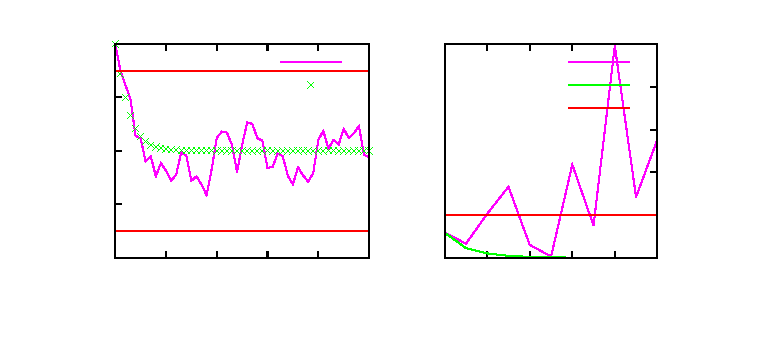
\includegraphics{mpc/CL1}}%
    \gplfronttext
  \end{picture}%
\endgroup
}
\caption{(Left) Closed-loop response (Right) Warm start rendered
  infeasible for actual state because of disturbance. The warm start
  is infeasible if $V_N^\beta(x,\tilde{\mathbf{v}})> \bar{V}$}
\label{fig:mpc:CL1}
\end{figure}


In Figure \ref{fig:mpc:CL2}, we show the closed-loop response using a
modified version of Algorithm \ref{alg:mpc:robust}. The modification we
made are to reset the nominal state to the actual state at time $k$ if the
following conditions are satisfied (i)The nominal state $z(k)$ is inside $\mathbb{Z}_f$.
(ii) The warm start $\tilde{\mathbf{v}}(k)$ is feasible for the
actual state $x(k)$ and , (iii) The time elapsed since the last reset
is greater than $\bar{T}$
time periods (we chose $\bar{T} = 10$)

\begin{figure}
\centering
\scriptsize
\resizebox{1\textwidth}{!}{% GNUPLOT: LaTeX picture with Postscript
\begingroup
  \makeatletter
  \providecommand\color[2][]{%
    \GenericError{(gnuplot) \space\space\space\@spaces}{%
      Package color not loaded in conjunction with
      terminal option `colourtext'%
    }{See the gnuplot documentation for explanation.%
    }{Either use 'blacktext' in gnuplot or load the package
      color.sty in LaTeX.}%
    \renewcommand\color[2][]{}%
  }%
  \providecommand\includegraphics[2][]{%
    \GenericError{(gnuplot) \space\space\space\@spaces}{%
      Package graphicx or graphics not loaded%
    }{See the gnuplot documentation for explanation.%
    }{The gnuplot epslatex terminal needs graphicx.sty or graphics.sty.}%
    \renewcommand\includegraphics[2][]{}%
  }%
  \providecommand\rotatebox[2]{#2}%
  \@ifundefined{ifGPcolor}{%
    \newif\ifGPcolor
    \GPcolortrue
  }{}%
  \@ifundefined{ifGPblacktext}{%
    \newif\ifGPblacktext
    \GPblacktexttrue
  }{}%
  % define a \g@addto@macro without @ in the name:
  \let\gplgaddtomacro\g@addto@macro
  % define empty templates for all commands taking text:
  \gdef\gplbacktext{}%
  \gdef\gplfronttext{}%
  \makeatother
  \ifGPblacktext
    % no textcolor at all
    \def\colorrgb#1{}%
    \def\colorgray#1{}%
  \else
    % gray or color?
    \ifGPcolor
      \def\colorrgb#1{\color[rgb]{#1}}%
      \def\colorgray#1{\color[gray]{#1}}%
      \expandafter\def\csname LTw\endcsname{\color{white}}%
      \expandafter\def\csname LTb\endcsname{\color{black}}%
      \expandafter\def\csname LTa\endcsname{\color{black}}%
      \expandafter\def\csname LT0\endcsname{\color[rgb]{1,0,0}}%
      \expandafter\def\csname LT1\endcsname{\color[rgb]{0,1,0}}%
      \expandafter\def\csname LT2\endcsname{\color[rgb]{0,0,1}}%
      \expandafter\def\csname LT3\endcsname{\color[rgb]{1,0,1}}%
      \expandafter\def\csname LT4\endcsname{\color[rgb]{0,1,1}}%
      \expandafter\def\csname LT5\endcsname{\color[rgb]{1,1,0}}%
      \expandafter\def\csname LT6\endcsname{\color[rgb]{0,0,0}}%
      \expandafter\def\csname LT7\endcsname{\color[rgb]{1,0.3,0}}%
      \expandafter\def\csname LT8\endcsname{\color[rgb]{0.5,0.5,0.5}}%
    \else
      % gray
      \def\colorrgb#1{\color{black}}%
      \def\colorgray#1{\color[gray]{#1}}%
      \expandafter\def\csname LTw\endcsname{\color{white}}%
      \expandafter\def\csname LTb\endcsname{\color{black}}%
      \expandafter\def\csname LTa\endcsname{\color{black}}%
      \expandafter\def\csname LT0\endcsname{\color{black}}%
      \expandafter\def\csname LT1\endcsname{\color{black}}%
      \expandafter\def\csname LT2\endcsname{\color{black}}%
      \expandafter\def\csname LT3\endcsname{\color{black}}%
      \expandafter\def\csname LT4\endcsname{\color{black}}%
      \expandafter\def\csname LT5\endcsname{\color{black}}%
      \expandafter\def\csname LT6\endcsname{\color{black}}%
      \expandafter\def\csname LT7\endcsname{\color{black}}%
      \expandafter\def\csname LT8\endcsname{\color{black}}%
    \fi
  \fi
  \setlength{\unitlength}{0.0500bp}%
  \begin{picture}(7200.00,3024.00)%
    \gplgaddtomacro\gplbacktext{%
      \csname LTb\endcsname%
      \put(814,704){\makebox(0,0)[r]{\strut{} 10}}%
      \put(814,1389){\makebox(0,0)[r]{\strut{} 20}}%
      \put(814,2074){\makebox(0,0)[r]{\strut{} 30}}%
      \put(814,2759){\makebox(0,0)[r]{\strut{} 40}}%
      \put(946,484){\makebox(0,0){\strut{} 0}}%
      \put(2898,484){\makebox(0,0){\strut{} 10}}%
      \put(4851,484){\makebox(0,0){\strut{} 20}}%
      \put(6803,484){\makebox(0,0){\strut{} 30}}%
      \put(176,1731){\rotatebox{-270}{\makebox(0,0){\strut{}Inventory at Retailer}}}%
      \put(3874,154){\makebox(0,0){\strut{}Time}}%
      \put(4851,1732){\makebox(0,0)[l]{\strut{}Nominal state reset}}%
    }%
    \gplgaddtomacro\gplfronttext{%
      \csname LTb\endcsname%
      \put(4037,877){\makebox(0,0)[r]{\strut{}Actual}}%
      \csname LTb\endcsname%
      \put(5816,877){\makebox(0,0)[r]{\strut{}Nominal}}%
    }%
    \gplbacktext
    \put(0,0){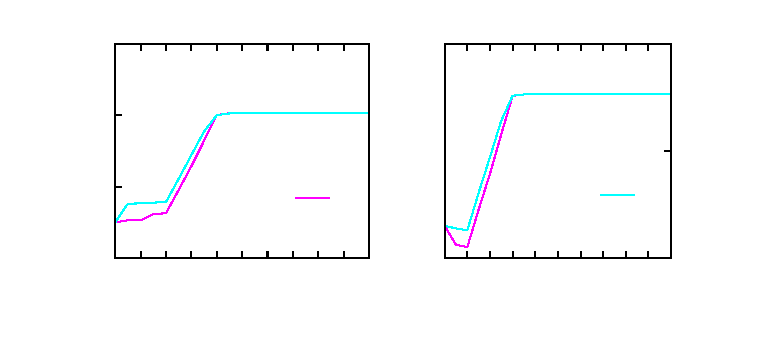
\includegraphics{CL2}}%
    \gplfronttext
  \end{picture}%
\endgroup
}
\caption{(Left) Closed-loop response. Notice that we reset the state
  around t = 15 (Right) Warm start rendered
  infeasible for actual state because of disturbance}
\label{fig:mpc:CL2}
\end{figure}





\section{Related Work}
\label{sec:mpc:related}
Cooperative MPC has evolved as an  attractive architecture for
distributed control because it solves the centralized control
problem, and inherits the desirable closed-loop properties of
centralized control. 
In the previous sections, we described
cooperative MPC based on the ``primal decomposition'' of the
centralized optimization
problem. In the primal decomposition, the centralized optimization
problem is solved directly using parallel optimization
architectures. \citet{liu:chen:pena:christofides:2010} also use the
primal decomposition to solve the centralized optimization problem for a
nonlinear process model. They use a closed-form controller $u=h(x)$
for which a Lyapunov function is known as a reference controller to
design their MPC optimization problem. Thus, they ensure that the MPC
inherits the stability properties of $u=h(x)$. Note that $u=h(x)$ also
provides a warm start, even when the actual and predicted states are
different. However, since this stability constraint is a coupled
constraint, there can be no guarantees about the convergence of the
parallel optimization routine to the optimal solution; and hence equivalence of optimal MPC
and cooperative MPC if the iterations were allowed to converge. The authors propose both a Jacobi
algorithm (all subsystems optimize in parallel) and a Gauss-Seidel
algorithm (subsystems optimize in sequence). In comparison, in
\citet{stewart:wright:rawlings:2011}, the authors propose a Jacobi
algorithm for nonlinear MPC that converges to the centralized optimal
solution. Since, for non-convex problems, the Jacobi optimizations
does not necessarily produce a descent direction, the authors propose
a sequential procedure to obtain a descent direction using the
solutions obtained from each subsystem. This overhead is not
equivalent to implementing a coordinator as each subsystem only
calculates an objective function in the second phase of the algorithm
in which a descent direction is
determined. \citet{maestre:pena:camacho:alamo:2011} propose a primal
decomposition approach to cooperative MPC based on agent
negotiation. The advantage of their procedure is that agents need only
know models of the subsystems whose inputs affect their states. In the
proposed method, each agent optimizes its local objective over all
the inputs that affect its dynamics, and share the proposed solution
with other agents. The other agents evaluate the proposal for
cost-drop and constraint violation and communicate back to the
original agent making the proposal, who can then decide to accept or
reject the proposal. The authors ensure that only feasible proposals
are accepted. The drawback of the proposed architecture, however, is
that (i) the agents have to solve larger optimization problems
(because they have to optimize over all the inputs that affect their
state), and (ii) the convergence to the centralized optimal solution
cannot be guaranteed. Stability is guaranteed using the warm
start. \citet{maestre:pena:camacho:2011} use game-theoretic analysis
to propose a distributed optimization framework. In this method, each
node, optimizes its local objective over its local decisions while
keeping the other subsystem decisions fixed. After completion of the
optimizations, the agents compute their local objectives for all
possible combinations of the overall system input (based on optimized
solution of the agents and the warm start). Upon sharing the
objectives, the agents then select the input that minimizes the
overall cost. Thus, each agent cooperatively makes a decision. However,
the proposed algorithm also fails to establish convergence to the
centralized optimal on iteration. Stability is guaranteed by design of
terminal region and warm-start. \citet{muller:revle:allgower:2012}
propose a optimization algorithm based on each node optimizing over
its local optimization problem. They use a terminal region which is a
sub-level set of the terminal penalty. Because of the presence of
coupled constraints, input directions are discarded if they are not
feasible, based on a check made after the optimizations. To ensure
cost-drop, the centralized objectives are also evaluated after the
optimizations and inputs that do not achieve cost-drop are
discarded. The model considered by the authors had coupling introduced
only via the constraints (both in the objective function and the
constraints). The authors also provide a method to define local time
varying terminal regions, so that the coupled terminal region
constraint is satisfied if each subsystem satisfies its local time
varying terminal region constraint. The algorithm provided by the
authors, satisfies the requirements of the optimizer for suboptimal
MPC, but again, does not give any  guarantee on convergence to the
optimal solution. The
requirement of decoupled dynamics is important in problems like multi
vehicle synchronization
etc. \citet{johansson:speranzon:johansson:johansson:2006} use a primal
decomposition to solve a multi-vehicle consensus problem as a MPC
problem. While the dynamics are decoupled, the consensus point,
similar to terminal equality constraint, is the complicating
constraint. Unlike the MPC problems where the objectives are also
constrained because of the dynamics, the multi-vehicle receding
horizon problem falls into the category of uncoupled objective but
coupled constraints. The author's use a primal decomposition which
generates feasible iterate that reduce the objective function
value. However, in order to ensure that the centralized optimal
solution is achieved, the authors use a coordinator, which is based on
sub-gradient optimization to handle the coupled constraint.

A common theme in optimizing the centralized  problem is
that it is not easy to guarantee convergence to the optimal
solution. However, stability can be guaranteed because every iterate
is designed so that it reduces the cost while remaining feasible. In
contrast, there are a lot of cooperative MPC algorithms which are
based on the ``dual decomposition''. In the dual decomposition, the
coupled constraints are relaxed by using the Lagrangian of the
optimization problem. For a fixed value of the Lagrange multipliers
(also called as prices or dual variables), the relaxed problem can be solved using
parallel optimization methods as there are no complicating
constraints. Upon achieving the solution to the relaxed problem, the
Lagrange multipliers are updated. The Lagrange multiplier update is
usually done by a coordinator. These algorithms often converge faster
to the optimal solution. However, their main disadvantage is that they
are guaranteed to produce a feasible iterate only upon
convergence. Since stability theory for suboptimal MPC rely on the
fact that the suboptimal iterate is feasible, cooperative MPC
algorithms using dual decomposition use stability theory based on
optimal MPC to ensure stability. Therefore, a common theme in dual
decomposition based cooperative MPC algorithms are a coordinator layer
and a requirement that the iterates converge. 

The cooperative MPC algorithms using dual decomposition differ based on
the technique used to update the dual variables. In
\citet{cheng:forbes:yip:2007}, the dual variables (prices) are updated
using a sub-gradient based optimization algorithm. Sub-gradient methods
are also used in \citet{ma:anderson:borrelli:2011},
\citet{wakasa:arakawa:tanka:akashi:2008},
\citet{marcos:forbes:guay:2009}. \citet{morocan:bourdais:dumur:buisson:2011}
formulate the building control problem as a MPC problem with linear
objectives and use Benders decomposition to solve the problem. Benders
decomposition is a widely popular parallel algorithm when by fixing the
value of a complicating variable, the remaining problem can be
completely separated. \citet{scheu:marquardt:2011} propose a dual
decomposition algorithm without a coordination layer. They augment the
local subsystem objective function with the sensitivity of the
objectives and constraints of other subsystems to obtain updates for
the dual variables along with the primal variables. However, this
method generates a feasible solution only upon
convergence. \citet{giselsson:doan:keviczky:schutter:rantzer:2012}, \citet{giselsson:rantzer:2010}
propose a dual decomposition algorithm with a stopping criteria based
on the objective value to ensure stability. They advocate the use of
long prediction horizon along with results obtained in
\citet{grune:2009} to determine bounds on the value of the objective
function so that stability can be
guaranteed. \citet{doan:keviczky:necoara:diehl:schutter:2009} modified
the Han's algorithm which is a dual decomposition based algorithm for
the special structure of the MPC problem. Although the method uses
communication between directly connected subsystems, stability is
guaranteed only upon convergence. \citet{necoara:doan:suykens:2008}
use a smoothing technique to simplify the dual problem. With the
smoothing technique, the coordinator problem for finding the Lagrange
multiplier updates becomes easier. The algorithm also gives bounds on
the number of iterations so that the optimal solution and constraint
violation are within a pre-specified limit ($\epsilon$ approximation of
the centralized problem). Finally, \citet{doan:keviczky:schutter:2011}, propose a primal feasible dual
gradient approach, that generates a primal feasible solution  that
achieves cost-drop in a
finite number of iterations based on an averaging scheme of the primal
variables at each iteration. 

\citet{christofides:scattolini:pena:liu:2012} is a recent review of different algorithms for distributed
MPC. \citet{necoara:nedelcu:dumitrache:2011} provides an excellent overview of the different
optimization problems and parallel solution strategies that are seen
in control and estimation.

\citet{trodden:richards:2006,trodden:richards:2007} propose a tube based robust distributed
MPC algorithm. In their method, at each sampling time, only one
subsystem performs optimization. The subsystem optimizes only over its
decision variables, keeping all other subsystem decisions fixed from
the previous iteration. This method is also an example of primal
decomposition. \citet{richards:how:2004} present a robust tube-based
MPC for systems with decoupled dynamics. The coupling constraints are
coupled output constraints. Their algorithm is based on the
Gauss-Seidel iterations.


%Special definitions
\chapter{A state space model for chemical production scheduling} 
\label{chap:scheduling}
%\paragraph{Note} Most of this chapter appears in
%\citet{subramanian:maravelias:rawlings:2012}.

In Chapter \ref{chap:mpc}, we discussed design of on-line
optimization problems for the control of dynamic systems using MPC, so
that the closed-loop has desirable properties like recursive
feasibility, asymptotic convergence. In this chapter, we employ
ideas from MPC to address iterative or rolling horizon scheduling
problems.
In Section \ref{sec:scheduling:introduction}, we provide an introduction to
the problem that we wish to address. In
Section~\ref{sec:scheduling:lit_review}, we give a brief background 
on chemical production scheduling and associated rescheduling
problems. In Section~\ref{sec:scheduling:state_space}, we derive the
state space model, including four types of disturbances. In
Section~\ref{sec:scheduling:example}, we present an example
illustrating the advantages of using terminal constraints in iterative
scheduling.

\section{Introduction \footnote{This text appears in Section 1 of
\citet{subramanian:maravelias:rawlings:2012}}}
\label{sec:scheduling:introduction}

Chemical production scheduling problems arise in a wide variety of
applications, from batch production  of pharmaceuticals and fine
chemicals to continuous production of bulk chemicals and oil refining
operations. To address these problems, research within the process
systems engineering (PSE) community has primarily focused on (i) the
formulation of models for a wide variety of scheduling problems, and
(ii) the development of scheduling algorithms. In terms of model
development, the emphasis has been on the accurate representation of
problems in a range of production environments as well as the modeling
of various processing characteristics and constraints (\eg utility
constraints, changeovers, transfer operations,
etc.)\citep{mendez:cerda:grossmann:harjunkoski:fahl:2006}. An aspect
that has received limited attention is how to design algorithms, based
on these models, for iterative scheduling.

Chemical production is an inherently dynamic process. A schedule has
to be revised when new information becomes available (new orders,
modified due dates, raw material availability etc.), and/or production
disturbances occur (\eg processing delays, unit breakdowns, process
unit availability, etc.). However, while some of the issues arising when scheduling is
performed iteratively have been discussed in contributions dealing
with rescheduling, scheduling is still thought of as a {\em{static}}
open-loop problem -- the goal is to obtain an optimal schedule for the
current state of the system based on current (and possibly some
forecast) data. The development of methods (models and solution
algorithms) for the closed-loop problem has received no
attention. Another limitation of existing rescheduling methods, as we
discuss in Section~\ref{sec:scheduling:lit_review:rescheduling}, is that they are
model specific and rely on the solution of a rescheduling model that
is generated  {\em{empirically}}.

The goal of this paper is to address some of the aforementioned
limitations employing ideas from the area of control and model
predictive control (MPC) in particular. Model predictive control
offers a natural framework for the study of dynamic problems. First,
it relies on a general representation of the underlying system,
including different types of disturbances, via the state space
model. Second, it offers results with regard to the quality of the
closed-loop performance of various control strategies. For example,
with careful design of the on-line optimization problem, features such
as recursive feasibility (feasibility of the optimization problem at
each sampling instance) and asymptotic stability (convergence to a
set-point for the nominal case) can be obtained. Interestingly, it has
been shown that simple re-optimization does not necessarily lead to
good closed-loop performance, as has been assumed in the scheduling
literature.

Towards this goal, we first transform a general
mixed-integer programming (MIP) scheduling model into a state space
model \eqref{eq:mpc:cent_model}. Second, we show how common scheduling
disruptions can me modeled as disturbances in the state space model,
and finally, we discuss how some concepts from MPC like terminal
constraints can be used in scheduling. 


\section{Background}
\label{sec:scheduling:lit_review}

\subsection{Chemical production scheduling problems and models\footnote{This text appears in Section 2.1 of
\citet{subramanian:maravelias:rawlings:2012}}}


Production scheduling is one of the many planning functions in a
manufacturing supply chain. The interactions of scheduling with other
functions along with capacity considerations determine the class of
scheduling problem. The interactions with demand and production
planning determine the type of scheduling problem to be solved (cyclic
vs. short-term). The types of decisions made at the scheduling level
are determined by the decisions made at the production planning
level. Also, capacity constraints often determine the objective
function (\eg throughput maximization vs. cost minimization). Finally,
input parameters to scheduling (\eg raw material availability) are
provided by other functions \citep{maravelias:sung:2009,
  maravelias:2012, stadtler:2005}.

In general, scheduling problems can be classified in terms of a
triplet $\alpha/\beta/\gamma$, where $\alpha$ denotes the
{\emph{production}} environment; $\beta$ denotes the processing
characteristics/constraints and $\gamma$ denotes the objective
function \citep{pinedo:2008}. The main production environments are
{\emph{sequential, network}} and {\emph{hybrid}}
\citep{maravelias:2012}. Note that different types of processing can
be present in the same facility. Processing characteristics and
constraints include setups, changeovers, release/due times, storage
constraints, material transfers, etc. Common objective functions are
the minimization of makespan, the minimization of production costs,
the maximization of throughput, and the minimization of weighted lateness.

The modeling approaches to chemical production scheduling can be
classified in terms of \citep{maravelias:2012}:

\begin{enumerate}
\item the decisions made at the scheduling level;
\item the entities used to express the scheduling model; and
\item the modeling of time.
\end{enumerate}

In the most general case, scheduling involves three types of
decisions: (i) batching (number and size of batches needed to satisfy
demand); (ii) assignment of batches (or tasks) to processing units;
and (iii) sequencing and/or timing of batches (tasks) on processing
units. If the batching decisions are fixed, then scheduling problems
are expressed in terms of batches (batch-based approach). If batching
decisions are made at the scheduling level, then materials and
material amounts are typically used to formulate the scheduling model
(material-based approach). Finally, the modeling of time includes
decisions at four levels: (i) selection between precedence and
grid-based approach; (ii) if precedence-based, selection between local
and global precedences; if time-grid based, selection between common
and unit specific grids; (iii) specific assumptions regarding the
precedence relationship between two tasks and the mapping of task onto
time; and (iv) selection between discrete and continuous time
representation \citep{maravelias:2012}.

In this paper we assume batching, unit-task assignment and
sequencing/timing decisions are all made at the scheduling level
(material-based approach). We further assume that the general
scheduling problem can be expressed in terms of production
{\em{tasks, units}}(unary resources), and
{\em{materials}}. While this type of formalism has been traditionally
used to express problems in network production environment,
\citet{sundaramoorthy:maravelias:2010} showed that it can also be
employed to represent problems in all production environments. A thorough discussion of the
various scheduling problems and modeling approaches is presented in
\citet{mendez:cerda:grossmann:harjunkoski:fahl:2006}.


\subsection{Reactive scheduling\footnote{This text appears in Section 2.4 of
\citet{subramanian:maravelias:rawlings:2012}.} }
\label{sec:scheduling:lit_review:rescheduling}


Rescheduling, or reactive scheduling, after observing disturbances to
the nominal schedule has attracted some research attention in the past
few years. \citet{smith:1995} emphasizes the process view of the
scheduling problem and outlines the following criteria for {\em{reactive
scheduling}}: (i) prioritize outstanding problem; (ii) identify
modifying goals; and (iii) estimate possibilities for efficient and
non-disruptive schedule modification. In the MIP-based approaches to
reactive scheduling, a nominal schedule is used in conjunction with a
MIP model to react to disturbances. On observing a disturbance,  part
of the schedule which has already been implemented is fixed and the
remainder of the scheduling horizon is re-optimized using
modifications to the original model to reflect the disturbances. Such
strategies were proposed by
\citet{vin:jeetmanyu:ierapetritou:2000,janak:floudas:kallrath:vormbrock:2006, 
relvas:matos:barbosa:fialho:2007},  
among others. \citet{novas:henning:2010} propose a constraint
programming based approach to locally repair the nominal
solution. \citet{mendez:cerda:2003} also propose a local repair
solution to the schedule based on a MIP formulation that considers the
current ``state'' of the plant, a nominal schedule and new
information. Motivated by rolling horizon optimization in process
control, several shrinking horizon and rolling horizon approaches to
the scheduling problem have also been proposed. For instance,
\citet{van:grossmann:2003} provide an example of a complex hydrogen
pipeline, in which they divide the planning horizon into planning
periods, and for each planning period, they solve the scheduling
problem in a shrinking horizon formulation. \citet{sand:engell:2004}
solve a two stage stochastic optimization problem to find robust
schedules. They employ a moving horizon framework in which the
decisions in the current time period, the first stage decisions are
implemented, while the second stage decisions are embedded in a
scenario tree for stochastic
variables. \citet{honkomp:mockus:reklaitis:1999} use an optimizer to
perform the scheduling in conjunction with a simulator to simulate
stochastic scenarios. \citet{rodrigues:gimeno:passos:campos:1996}
propose a rolling horizon reactive scheduling method in which they
provide a predictive framework to determine future infeasibilities that
lie outside the current optimization
horizon. \citet{huercio:espuna:puigjaner:1995} present heuristics for
rescheduling based on shifting of task processing times and
reassignment of tasks to other units. \citet{li:ierapetritou:2008a}
propose a multi-parametric approach to rescheduling.
\citet{munawar:gudi:2005} propose a three level decomposition of the
problem, and motivated by process control, formulate feedback and
cascade control-like solutions to reactive
scheduling. \citet{li:ierapetritou:2008b} present a review of
different strategies used in reactive
scheduling. \citet{verderame:elia:li:floudas:2010} also present a
review of different approaches taken in different industries.



\section{State space scheduling model}
\label{sec:scheduling:state_space}

\subsection{General problem statement\footnote{ This text appears in Section 2.2 of
\citet{subramanian:maravelias:rawlings:2012}.}}


The scheduling problem we consider is stated as follows. We are given:
\begin{enumerate}
\item A set of processing tasks $i \in \mathbf{I}$; the processing time of
task $i$ is denoted by $\tilde{\tau}_i$, its fixed batchsize by
$\beta_i$ (variable batchsizes are considered in
Section~\ref{sec:scheduling:state_space:extensions}), and its production
cost by $\gamma_i$. Tasks that can be performed on many units are
modeled as different tasks, each one carried out only in one unit.
\item A set of equipment units $j \in \mathbf{J}$. The subset of tasks
  $i$ that can be carried out in unit $j$ is denoted by the set
  $\mathbf{I}_j$.
\item A set of materials $k \in \mathbf{K}$ stored in dedicated
  storage vessels of capacity $\sigma_k$. The unit inventory cost of
  $k$ is $\nu_k$. The set of tasks $i$ that produce/consume $k$ is
  denoted by $\mathbf{I}_k^+$/$\mathbf{I}_k^{-}$. Task $i$
  consumes/produces $\rho_{ik}$ units of material $k$ per unit of
  batchsize $\beta_i$. 
\item A set of shipments, $l \in \mathbf{L}$ (deliveries of feedstocks
  $k \in \mathbf{K}^F \subset \mathbf{K}$ or order for products $k \in
  \mathbf{K}^P \subset \mathbf{K}$); $\tilde{\phi}_l$ is the release
  (due) time of delivery (order) $l$; and $\zeta_l$ is the amount
  delivered ($\zeta_l > 0$) or due ($\zeta_l < 0$). $\mathbf{L}_k$ is
  the set of shipments (deliveries or orders) of material $k$. 
\end{enumerate}

Our goal is to meet the orders for the final products at the minimum
total cost. Other objective functions can also be considered.

If a task has no input or output material (\eg when two consecutive
tasks are carried out on the same unit), dummy materials can be
introduced to model the sequence of tasks. Also, if material amounts
need not be monitored (\eg sequential processes with fixed batchsize),
then we assume a nominal batchsize of 1 and unit conversion
coefficients. Note that we use the term {\emph{material}} instead of
{\emph{state}}, because the latter has a different meaning in
state space models. Raw time-related data, $\tilde{\tau}_i$ and
$\tilde{\phi}_l$ are given in regular time units (\eg hours), and are
represented by parameters with a tilde.

\subsection{Scheduling MIP model\footnote{This text appears in Section 2.3 of
\citet{subramanian:maravelias:rawlings:2012}}}

 
We consider a discrete-time model, in which the time horizon $\eta$,
is divided into $T$ periods of fixed length $\delta = \eta/T$,
defining $t+1$ time points, where period $t$ starts(ends) at time
point $t-1(t)$ \citep{shah:pantelides:sargent:1993}. We use time index
$t \in \mathbf{T}$ to denote both time point and periods. Time-related
data are scaled using $\delta$ and approximated so that the resulting
solutions are feasible. Specifically, processing times are rounded up,
$\tau_i = \lceil \tilde{\tau}_i/\delta \rceil$; and release and due
times are approximated conservatively, $\phi_l = \lceil
\tilde{\phi}_l/\delta \rceil$ if $\gamma_l >0$ and, $\phi_l = \lfloor
\tilde{\phi}_l/\delta \rfloor$ if $\gamma_l <0$. We also generate the
set of shipments for material $k$ at time $t$, $\mathbf{L}_{kt} = \set{l
  \in \mathbf{L}_k \mid \phi_l=t}$; and then calculate the total
shipment of material $k$ at time $t$:
\[ \xi_{kt} = \sum_{l \in \mathbf{L}_{kt}} \zeta_l, \qquad \forall k,t
\]
The optimizing decisions are $W_{i,t} \in \set{0,1}$ which is one if
task $i$ is assigned to start on unit $j$ at time point $t$; and
$S_{k,t} \geq 0$ , which is the inventory of material $k$ during time
period $t$. Any feasible schedule should satisfy the assignment
constraint  \eqref{eq:scheduling:assign} that expresses that at most
one task can be executed on a  unit at a time.
\begin{equation}
\label{eq:scheduling:assign}
\sum_{i \in \mathbf{I}_j}\sum_{t'=t-\tau_i+1}^{t} W_{i,t'} \leq 1,
\qquad \forall j,t
\end{equation}

If we assume that the orders are satisfied on time, the following
material balance gives the inventory variables:
\begin{equation}
\label{eq:scheduling:inventoryBalance}
S_{k,t+1} = S_{k,t} + \sum_{i\in
  \mathbf{I}_k^+}\rho_{ik}\beta_iW_{i,t-\tau_i} + \sum_{i \in
  \mathbf{I}_k^-}\rho_{ik}\beta_iW_{i,t}+ \xi_{kt} \leq \sigma_{k},
\qquad \forall k,t
\end{equation}

The objective function is 
\begin{equation}
\label{eq:scheduling:objective}
z = \min_{}{\sum_{i,t} \gamma_i W_{i,t} + \sum_{k,t}\nu_kS_{k,t}}
\end{equation}

The basic scheduling model $\mathbf{M}^{\text{SCH}}$ we consider
consists of Equations
\eqref{eq:scheduling:assign}--\eqref{eq:scheduling:objective}, with
$W_{i,t} \in \set{0,1}, \forall i,t$ and $S_{k,t} \in
[0,\sigma_k]. \forall k,t$.

If orders cannot be met on time (or we do not wish to meet them), then
we can introduce backorders variable and an additional equation for
its calculation. 

A simple problem
with one unit, two tasks and three materials, and the associated data
are shown in
Figure~\ref{fig:scheduling:ABexample}. Figure~\ref{fig:scheduling:ABgantt}
shows a solution to this problem-a Gantt chart showing the execution
of the tasks and the inventory profiles of the three materials. We use
this example throughout this chapter to illustrate the basic ideas.

\begin{figure}
  \centering
  \resizebox{0.5\columnwidth}{!}{\begin{picture}(0,0)%
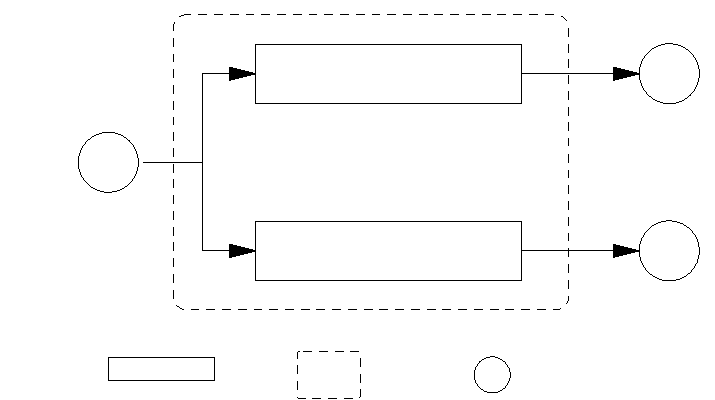
\includegraphics{scheduling/ABexample}%
\end{picture}%
\setlength{\unitlength}{4144sp}%
%
\begingroup\makeatletter\ifx\SetFigFont\undefined%
\gdef\SetFigFont#1#2#3#4#5{%
  \reset@font\fontsize{#1}{#2pt}%
  \fontfamily{#3}\fontseries{#4}\fontshape{#5}%
  \selectfont}%
\fi\endgroup%
\begin{picture}(5430,3041)(76,-3447)
\put( 91,-1726){\makebox(0,0)[lb]{\smash{{\SetFigFont{17}{20.4}{\rmdefault}{\mddefault}{\updefault}{\color[rgb]{0,.56,0}RM}%
}}}}
\put(3061,-3301){\makebox(0,0)[lb]{\smash{{\SetFigFont{17}{20.4}{\rmdefault}{\mddefault}{\updefault}{\color[rgb]{0,0,0}Unit}%
}}}}
\put(4141,-3301){\makebox(0,0)[lb]{\smash{{\SetFigFont{17}{20.4}{\rmdefault}{\mddefault}{\updefault}{\color[rgb]{0,0,0}Material}%
}}}}
\put(1801,-3301){\makebox(0,0)[lb]{\smash{{\SetFigFont{17}{20.4}{\rmdefault}{\mddefault}{\updefault}{\color[rgb]{0,0,0}Task}%
}}}}
\put(2971,-1051){\makebox(0,0)[lb]{\smash{{\SetFigFont{17}{20.4}{\rmdefault}{\mddefault}{\updefault}{\color[rgb]{0,0,0}TA}%
}}}}
\put(2971,-2401){\makebox(0,0)[lb]{\smash{{\SetFigFont{17}{20.4}{\rmdefault}{\mddefault}{\updefault}{\color[rgb]{0,0,0}TB}%
}}}}
\put(1126,-556){\makebox(0,0)[lb]{\smash{{\SetFigFont{17}{20.4}{\rmdefault}{\mddefault}{\updefault}{\color[rgb]{0,0,0}U}%
}}}}
\put(1801,-1996){\makebox(0,0)[lb]{\smash{{\SetFigFont{17}{20.4}{\rmdefault}{\mddefault}{\updefault}{\color[rgb]{0,0,0}$\tau_{TB}=2$hr, $\beta_{TB}=6$ton}%
}}}}
\put(1801,-1411){\makebox(0,0)[lb]{\smash{{\SetFigFont{17}{20.4}{\rmdefault}{\mddefault}{\updefault}{\color[rgb]{0,0,0}$\tau_{TA}=3$hr, $\beta_{TA}=4$ton }%
}}}}
\put(5491,-2401){\makebox(0,0)[lb]{\smash{{\SetFigFont{17}{20.4}{\rmdefault}{\mddefault}{\updefault}{\color[rgb]{1,0,0}$B$}%
}}}}
\put(5491,-1006){\makebox(0,0)[lb]{\smash{{\SetFigFont{17}{20.4}{\rmdefault}{\mddefault}{\updefault}{\color[rgb]{0,0,1}$A$}%
}}}}
\end{picture}%
}
  \caption{Simple scheduling problem}
  \label{fig:scheduling:ABexample}
\end{figure}

\begin{figure}[h]
  \centering
  \resizebox{0.5\columnwidth}{!}{\begin{picture}(0,0)%
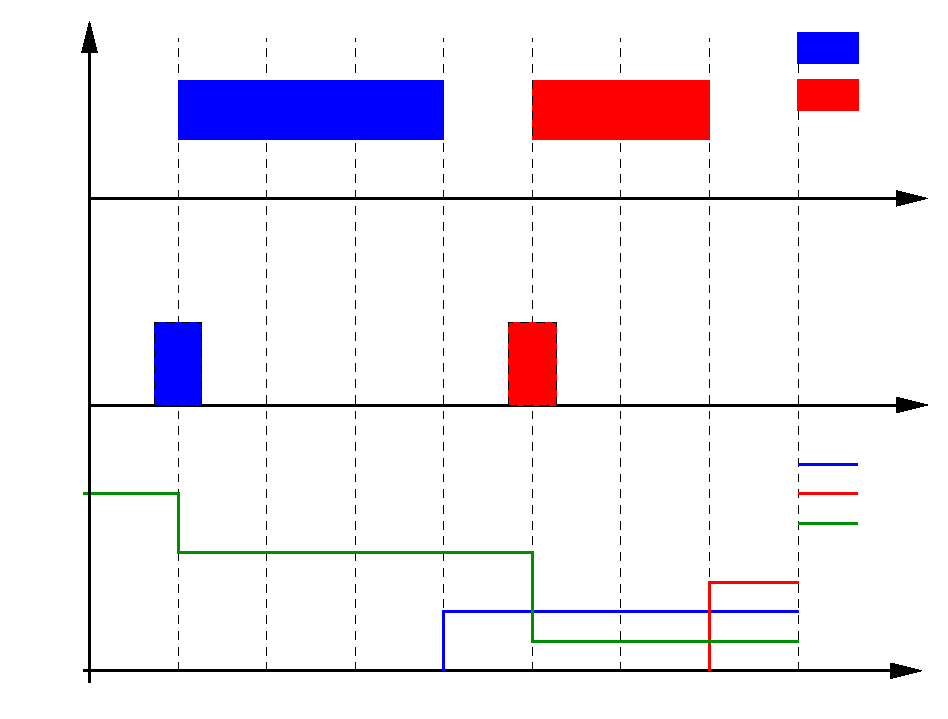
\includegraphics{scheduling/ABgantt}%
\end{picture}%
\setlength{\unitlength}{4144sp}%
%
\begingroup\makeatletter\ifx\SetFigFont\undefined%
\gdef\SetFigFont#1#2#3#4#5{%
  \reset@font\fontsize{#1}{#2pt}%
  \fontfamily{#3}\fontseries{#4}\fontshape{#5}%
  \selectfont}%
\fi\endgroup%
\begin{picture}(6967,5212)(1471,-5476)
\put(2926,-2536){\makebox(0,0)[lb]{\smash{{\SetFigFont{17}{20.4}{\rmdefault}{\mddefault}{\updefault}{\color[rgb]{0,0,0}$W_{TA,1}=1$}%
}}}}
\put(2701,-421){\makebox(0,0)[lb]{\smash{{\SetFigFont{17}{20.4}{\rmdefault}{\mddefault}{\updefault}{\color[rgb]{0,0,0}Gantt Chart}%
}}}}
\put(2701,-3571){\makebox(0,0)[lb]{\smash{{\SetFigFont{17}{20.4}{\rmdefault}{\mddefault}{\updefault}{\color[rgb]{0,0,0}Inventory profile}%
}}}}
\put(8101,-556){\makebox(0,0)[lb]{\smash{{\SetFigFont{17}{20.4}{\rmdefault}{\mddefault}{\updefault}{\color[rgb]{0,0,0}TA}%
}}}}
\put(8101,-916){\makebox(0,0)[lb]{\smash{{\SetFigFont{17}{20.4}{\rmdefault}{\mddefault}{\updefault}{\color[rgb]{0,0,0}TB}%
}}}}
\put(7966,-3706){\makebox(0,0)[lb]{\smash{{\SetFigFont{17}{20.4}{\rmdefault}{\mddefault}{\updefault}{\color[rgb]{0,0,0}$S_{A,t}$}%
}}}}
\put(7966,-3931){\makebox(0,0)[lb]{\smash{{\SetFigFont{17}{20.4}{\rmdefault}{\mddefault}{\updefault}{\color[rgb]{0,0,0}$S_{B,t}$}%
}}}}
\put(7966,-4156){\makebox(0,0)[lb]{\smash{{\SetFigFont{17}{20.4}{\rmdefault}{\mddefault}{\updefault}{\color[rgb]{0,0,0}$S_{RM,t}$}%
}}}}
\put(1486,-2356){\makebox(0,0)[lb]{\smash{{\SetFigFont{17}{20.4}{\rmdefault}{\mddefault}{\updefault}{\color[rgb]{0,0,0}$W_{i,t}$}%
}}}}
\put(7831,-5461){\makebox(0,0)[lb]{\smash{{\SetFigFont{17}{20.4}{\rmdefault}{\mddefault}{\updefault}{\color[rgb]{0,0,0}Time}%
}}}}
\put(3376,-5416){\makebox(0,0)[lb]{\smash{{\SetFigFont{17}{20.4}{\rmdefault}{\mddefault}{\updefault}{\color[rgb]{0,0,0}2}%
}}}}
\put(4726,-5416){\makebox(0,0)[lb]{\smash{{\SetFigFont{17}{20.4}{\rmdefault}{\mddefault}{\updefault}{\color[rgb]{0,0,0}4}%
}}}}
\put(6076,-5416){\makebox(0,0)[lb]{\smash{{\SetFigFont{17}{20.4}{\rmdefault}{\mddefault}{\updefault}{\color[rgb]{0,0,0}6}%
}}}}
\put(7426,-5416){\makebox(0,0)[lb]{\smash{{\SetFigFont{17}{20.4}{\rmdefault}{\mddefault}{\updefault}{\color[rgb]{0,0,0}8}%
}}}}
\put(5626,-2536){\makebox(0,0)[lb]{\smash{{\SetFigFont{17}{20.4}{\rmdefault}{\mddefault}{\updefault}{\color[rgb]{0,0,0}$W_{TB,5}=1$}%
}}}}
\end{picture}%
}
  \caption{Scheduling solution}
  \label{fig:scheduling:ABgantt}
\end{figure}


\subsection{Inputs and states\footnote{This section corresponds to the model developed in Section 3.1 of
  \citet{subramanian:maravelias:rawlings:2012}.}}
 
%\paragraph{Note:} This text appears in Section 3.1 of
%\citet{subramanian:maravelias:rawlings:2012}. 

Since assignment variables $W_{i,t}$ are the main scheduling
decisions; they are the inputs in the state space realization of $\mathbf{M}^{\text{SCH}}$. Inventory
levels $S_{k,t}$ in $\mathbf{M}^{\text{SCH}}$ are determined by
$W_{i,t}$ and the inventory balance dynamics, and hence are states. However, the
variables $S_{k,t}$ do not completely describe the state of the
system. Consider the solution shown in Figure
\ref{fig:scheduling:ABgantt}. The variables $W_{\text{TA},2}$ and
$W_{\text{TA},3}$  are both zero, but at $t=2$, the task TA has run for
one hour while at $t=3$, the task TA has run for two hours. Therefore,
to completely describe the state of the system, the history of the
system should also be included in the system state. This is achieved
through {\em{lifting}}.  We define the new state variables
$\bar{W}_{i,t}^{n}$ to carry past decisions to $t$. The state variable
$\bar{W}_{i,t}^{n} = 1$ indicates that a batch of task $i$ started at
time $t-n$. The lifted equations are given by:
\begin{align}
\label{eq:scheduling:liftedW}
\bar{W}_{i,t+1}^{1} &= W_{i,t} \nonumber \\
\bar{W}_{i,t+1}^{n} &= \bar{W}_{i,t}^{n-1} \quad \forall n \in
\set{2,3,\ldots,\tau_i}  
\end{align}

Using the lifted states, the inventory balance equation
\eqref{eq:scheduling:inventoryBalance} can be written as:

\begin{equation}
\label{eq:scheduling:x}
S_{k,t+1} = S_{k,t} + \sum_{i\in
  \mathbf{I}_k^+}\rho_{ik}\beta_i\bar{W}_{i,t}^{\tau_i} + \sum_{i\in
  \mathbf{I}_k^-}\rho_{ik}\beta_iW_{i,t}+ \xi_{k,t} \qquad \forall k,t
\end{equation}

Similarly, the assignment constraint \eqref{eq:scheduling:assign} can
be written as
\begin{equation}
\label{eq:scheduling:constraint}
\sum_{i \in \mathbf{I}_j} W_{i,t} + \sum_{i \in \mathbf{I}_j}
\sum_{n=1}^{\tau_i-1}\bar{W}_{i,t}^{n} \leq 
1 \qquad \forall j,t
\end{equation}

Defining the state $x(t) = \begin{bmatrix}S_{k,t}, k \in \mathbf{K}, &
\bar{W}_{i,t}^{n}, i \in \mathbf{I}, n \in
\set{1,2,\ldots,\tau_i} \end{bmatrix}$, the input $u(t)
= \begin{bmatrix} W_{i,t}, i \in \mathbf{I}\end{bmatrix}$ and the 
disturbance $d(t) = \begin{bmatrix} \xi_{k,t}, k \in
  \mathbf{K}\end{bmatrix}$, we can write the 
  scheduling model in the familiar state space form $x(k+1) = 
Ax(k)+Bu(k)+B_dd(k)$. Equations \eqref{eq:scheduling:liftedW} and 
\eqref{eq:scheduling:x} express the dynamic evolution of the system, 
and Equation \eqref{eq:scheduling:constraint} is a joint state-input
constraint. The objective function can be easily written as the sum of
economic stage costs $\ell_E(x,u) = q'x+r'u$.

The dynamic evolution, constraints and stage costs for the simple
scheduling model introduced in Figure \ref{fig:scheduling:ABexample}
are given in Equations
\eqref{eq:scheduling:ABss}--\eqref{eq:scheduling:ABstage_cost}.


\begin{equation}
\label{eq:scheduling:ABss}
\begin{bmatrix}S_{\text{RM}}\\S_A\\S_B\\\bar{W}_{\text{TA}}^1\\ 
\bar{W}_{\text{TA}}^2\\\bar{W}_{\text{TA}}^3\\\bar{W}_{\text{TB}}^1
\\\bar{W}_{\text{TB}}^2\end{bmatrix}_{t+1}
= \underbrace{\begin{bmatrix}
 1& & & & & & & \\
 &1 & & & &\beta_{\text{TA}} & & \\ 
 & &1 & & & & &\beta_{\text{TB}} \\
 & & & & & & & \\
 & & & &1 & & & \\
 & & & & &1 & & \\
 & & & & & & & \\
 & & & & & &1
 & \end{bmatrix}}_{A}\underbrace{\begin{bmatrix}S_{\text{RM}}\\
S_A\\S_B\\\bar{W}_{\text{TA}}^1\\\bar{W}_{\text{TA}}^2\\
\bar{W}_{\text{TA}}^3\\\bar{W}_{\text{TB}}^1\\
\bar{W}_{\text{TB}}^2\end{bmatrix}_{t}}_{x(t)}+
\underbrace{
\begin{bmatrix}
-\beta_{\text{TA}} & -\beta_{\text{TB}}\\
 & \\
 & \\
1 & \\
 & \\
 & \\
 &1 \\
 & \end{bmatrix}
}_{B}\underbrace{\begin{bmatrix}W_{\text{TA}}
    \\W_{\text{TB}}\end{bmatrix}_{t}}_{u(t)} +
\underbrace{
\begin{bmatrix}
 & \\
1 & \\
 &1 \\
 & \\
 & \\
 & \\
 &\\
 & \end{bmatrix}
}_{B_d}\underbrace{\begin{bmatrix}\xi_{A}\\\xi_{B}\end{bmatrix}_{t}}_{d(t)} 
\end{equation}

\begin{equation}
\label{eq:scheduling:ABconst}
\begin{bmatrix} 0 \\ 0 \\ 0\\ 0 \end{bmatrix} \leq
\underbrace{
\begin{bmatrix}
1& & & & & & & \\
 &1& & & & & & \\
 & &1& & & & & \\
 & & &1&1& &1& \end{bmatrix}   
}_{E_x}
\begin{bmatrix}S_{\text{RM}}\\S_A\\S_B\\
\bar{W}_{\text{TA}}^1\\\bar{W}_{\text{TA}}^2\\
\bar{W}_{\text{TA}}^3\\\bar{W}_{\text{TB}}^1\\
\bar{W}_{\text{TB}}^2\end{bmatrix}_{t}+
\underbrace{
\begin{bmatrix}
 & \\
 & \\
 & \\
1& 1 \end{bmatrix}
}_{E_u}\begin{bmatrix}W_{\text{TA}}
    \\W_{\text{TB}}\end{bmatrix}_{t} \leq 
\begin{bmatrix}\sigma_{\text{RM}}\\\sigma_{A}\\
\sigma_{B}\\1\end{bmatrix}
\end{equation}
\begin{equation}
\label{eq:scheduling:ABstage_cost}
\ell_E(x,u)
= \underbrace{\begin{bmatrix}\nu_{\text{RM}} & \nu_A & \nu_B & & &
  & \end{bmatrix}}_{q'}\begin{bmatrix}S_{\text{RM}}\\
S_A\\S_B\\\bar{W}_{\text{TA}}^1\\  
\bar{W}_{\text{TA}}^2\\\bar{W}_{\text{TA}}^3\\
\bar{W}_{\text{TB}}^1\\\bar{W}_{\text{TB}}^2\end{bmatrix}_{t}+   
\underbrace{\begin{bmatrix}\gamma_{\text{TA}} 
  & \gamma_{\text{TB}} \end{bmatrix}}_{r'}\begin{bmatrix}W_{\text{TA}}
    \\W_{\text{TB}}\end{bmatrix}_{t}
\end{equation}

\subsection{Disturbances\footnote{This section corresponds to the model developed in Section 3.1 of
  \citet{subramanian:maravelias:rawlings:2012}.} }

Events that can lead to rescheduling are modeled as disturbances. We
have already discussed shipments as a disturbance in the previous
section. In this section, we model three disturbances, namely, task yields, task
delays and unit breakdowns. 

\subsubsection{Shipments}
We assume that backorders are not allowed. Therefore, the shipping
schedule is fixed by customer orders. Hence, shipments are treated as
disturbances. We denote the nominal customer demands as
${\xi}_{k,t}^{\text{nom}}$. Shipment disturbances are deviations
$\hat{\xi}_{k,t}$ from the nominal value. That is,
\[ \xi_{k,t} = \xi_{k,t}^{\text{nom}} + \hat{\xi}_{k,t} \] 


\subsubsection{Task yields}
Consumption and production disturbances are used to model changes in
yields and losses during loading and
unloading. We define  yield disturbance variables $\beta_{i,k,t}^P$
and $\beta_{i,k,t}^C$ to denote deviation from the nominal
production/consumption of material $k$ by a batch of task $i$
finishing/starting at time $t$. For example, $\beta_{i,k,t}^P < 0$
indicates lower yield than the nominal batch size. The material
balance equations \eqref{eq:scheduling:x} is now modified as :

\begin{equation}
\label{eq:scheduling:yield_loss}
S_{k,t+1} = S_{k,t} + \sum_{i\in
  \mathbf{I}_k^+}\rho_{ik}\beta_i\bar{W}_{i,t}^{\tau_i} + \sum_{i\in
  \mathbf{I}_k^-}\rho_{ik}\beta_iW_{i,t}+ \left(\xi_{k,t} + \sum_{i\in
  \mathbf{I}_k^+}\rho_{ik}\beta_{i,k,t}^{P} +\sum_{i\in
  \mathbf{I}_k^-}\rho_{ik}\beta_{i,k,t}^{C}\right)    \qquad \forall k,t
\end{equation}

\subsubsection{Task delays}
We introduce
disturbance variable $\hat{Y}_{i,t}^{n}$ to model delays during the
execution of a task. The variable $\hat{Y}_{i,t}^{n} = 1$ when an 1-period delay
($\delta$ h) of task $i$ occurring $n$ periods after task $i$
started has been observed. The state equations ~\eqref{eq:scheduling:liftedW} are corrected as:

\begin{align}
\label{eq:scheduling:task_delay_W}
\bar{W}_{i,t+1}^{1} &= W_{i,t} - \hat{Y}_{i,t} \nonumber \\
\bar{W}_{i,t+1}^{n} &= \bar{W}_{i,t}^{n-1} + \hat{Y}_{i,t}^{n} -
\hat{Y}_{i,t}^{n-1},\qquad \forall i,t,n \in \set{2,3,\ldots,\tau_i}
\end{align}

Equation \eqref{eq:scheduling:task_delay_W} essentially says that the
values of states $\bar{W}_{i,t+1}^{n}$ should be the same as
$\bar{W}_{i,t}^{n}$ if there is a 1-period delay at $t$.  The state
equations \eqref{eq:scheduling:x} is corrected as:

\begin{equation}
\label{eq:scheduling:task_delay_S}
S_{k,t+1} = S_{k,t} + \sum_{i\in
  \mathbf{I}_k^+}\rho_{ik}\beta_i\bar{W}_{i,t}^{\tau_i} + \sum_{i\in
  \mathbf{I}_k^-}\rho_{ik}\beta_iW_{i,t}+ \xi_{k,t} - \sum_{i\in
  \mathbf{I}_k^+}\rho_{ik}\beta_i\hat{Y}_{i,t}^{\tau_i}    \qquad \forall k,t
\end{equation}

For example, consider the situation in which the task $\text{TA}$ was
started at $t=1$. Hence $W_{\text{TA},1} = 1$. The state equation
\eqref{eq:scheduling:liftedW}, then implies that
$\bar{W}_{\text{TA},3}^{2} = 1$, as at $t=3$, the task $\text{TA}$ has
been running for $2$ hours. If a 1-period delay is observed at time
$t=3$, then the variable $\hat{Y}_{\text{TA},3}^{2} = 1$. This means that
instead of finishing at $t=4$, the task gets completed only at
$t=5$. Hence, for modeling purpose, the task started only at time
$t=2$. In rescheduling literature, a new model is written with this
information, i.e., $W_{\text{TA},2}=1, W_{\text{TA},1}=0$. In our
proposed method, such delays are handled organically by modifying the
lifted states. Equation \eqref{eq:scheduling:task_delay_W} tells us
that
\[ \bar{W}_{\text{TA},4}^{3} = \bar{W}_{\text{TA},3}^{2} +
\hat{Y}_{\text{TA},3}^{3} -\hat{Y}_{\text{TA},3}^{2} = 1+0 -1 = 0 \]
and 
\[ \bar{W}_{\text{TA},4}^{2} = \bar{W}_{\text{TA},3}^{1} +
\hat{Y}_{\text{TA},3}^{2} -\hat{Y}_{\text{TA},3}^{1} = 0+1-0 = 1\]
Hence, we can verify that the disturbance variable $\hat{Y}_{i,t}^{n}$
successfully models an 1-period delay. 

\subsubsection{Unit breakdowns}
In contrast to a  task delay, a unit breakdown leads to the termination of the
task being executed on the unit at the time of the breakdown. In such
an event, all production in that unit is also lost.  To model a breakdown of unit $j$, we introduce
disturbance variable $\hat{Z}_{i,t}^{n}$. The variable
$\hat{Z}_{i,t}^{n} = 1$ when a breakdown (of duration 1 period)
occurring $n$ hours after task $i \in \mathbf{I}_j$ started is observed.
Unlike the previous section, we force all the lifted variables
affected by the shutdown to be zero as:
\begin{align}
\label{eq:scheduling:breakdown_W}
\bar{W}_{i,t+1}^{1} &= W_{i,t} - \hat{Z}_{i,t} \nonumber\\
\bar{W}_{i,t+1}^{n} &= \bar{W}_{i,t}^{n-1} - \hat{Z}_{i,t}^{n-1} \qquad
\forall i, n \in \set{2,3,\ldots,\tau_i}
\end{align}

The  state equations \eqref{eq:scheduling:x} is corrected as
\begin{equation}
\label{eq:scheduling:breakdown_S}
S_{k,t+1} = S_{k,t} + \sum_{i \in
  \mathbf{I}_k^+}\rho_{ik}\beta_i\bar{W}_{i,t}^{\tau_i} + \sum_{i\in
  \mathbf{I}_k^-}\rho_{ik}\beta_iW_{i,t}+ \xi_{k,t} - \sum_{i\in
  \mathbf{I}_k^+}\rho_{ik}\beta_i\hat{Z}_{i,t}^{\tau_i}    \qquad \forall k,t
\end{equation}

Finally, to ensure that no tasks are assigned to unit $j$ if it is out
of order, the constraint \eqref{eq:scheduling:constraint} is modified as:

\begin{equation}
\label{eq:scheduling:breakdown_constraint}
\sum_{i \in \mathbf{I}_j} W_{i,t} + \sum_{i \in \mathbf{I}_j}
\sum_{n=1}^{\tau_i-1}\bar{W}_{i,t}^{n} +\sum_{i \in \mathbf{I}_j}
\sum_{n=1}^{\tau_i-1}\hat{Z}_{i,t}^{n}  + \hat{Z}_{i,t} \leq 
1 \qquad \forall j,t
\end{equation}

A breakdown lasting multiple periods, from $t$ to $t+\phi$ can be
modeled as consecutive 1 period breakdowns. Since the subsequent
breakdowns occur while no task is executed, we introduce an idle task
$\text{IT}(j) \forall j$ with $ \tau_{\text{IT}(j)} = 1$ and use
$\hat{Z}_{\text{IT}(j),t+1}^{1} = \hat{Z}_{\text{IT}(j),t+2}^{2} =
\ldots = \hat{Z}_{\text{IT}(j),t+\phi}^{1} = 1$. 

\subsection{Final model}
 

The final state space scheduling model includes the state evolution
described by \eqref{eq:scheduling:finalSS} and the modified
constraint given by \eqref{eq:scheduling:breakdown_constraint}. 

\begin{xalignat}{2}
\label{eq:scheduling:finalSS}
\bar{W}_{i,t+1}^{1} &= W_{i,t} - \hat{Z}_{i,t} - \hat{Y}_{i,t} &
\forall i,t \nonumber\\ 
\bar{W}_{i,t+1}^{n} & = \bar{W}_{i,t}^{n-1}
-\hat{Z}_{i,t}^{n-1}+\hat{Y}_{i,t}^n-\hat{Y}_{i,t}^{n-1}&  \forall i,t,n\in
\set{2,3,\ldots,\tau_i} \\
S_{k,t+1} &= S_{k,t} + \sum_{i \in
  \mathbf{I}_k^+}\rho_{ik}\beta_i\bar{W}_{i,t}^{\tau_i} + \sum_{i\in
  \mathbf{I}_k^-}\rho_{ik}\beta_iW_{i,t}+ &\nonumber \\ & \left(
  \xi_{k,t} - \sum_{i\in 
  \mathbf{I}_k^+}\rho_{ik}\left(\beta_i(\hat{Z}_{i,t}^{\tau_i}
  -\hat{Y}_{i,t}^{\tau_i})+\beta_{i,k,t}^P\right) + \sum_{i\in
  \mathbf{I}_k^-} \rho_{ik}\beta_{i,k,t}^C\right)&  \forall k,t \nonumber
\end{xalignat}

With the disturbance \[d(t) = \begin{bmatrix} \xi_{k,t}, k \in
  \mathbf{K}, & \beta_{i,k,t}^P, \beta_{i,k,t}^C, i \in \mathbf{I}, k
  \in \mathbf{K},& \hat{Y}_{i,t}, \hat{Y}_{i,t}^{n}, \hat{Z}_{i,t},
  \hat{Z}_{i,t}^{n}, i \in 
  \mathbf{I}, n \in \set{2,3,\ldots,\tau_i}\end{bmatrix}\]
the final model can be written in the state space form. In the general
case, we have $ u \in \set{0,1}^m$ in which $m = \norm{\mathbf{I}}$;
$x \in \mathbb{R}^{n_c} \times \set {0,1}^{n_b}$ in which $n_c =
\norm{\mathbf{S}}$ and $n_b = \sum_{i \in \mathbf{I}} \tau_i$; and $d
\in \mathbb{R}^{n_d} \times \set{0,1}^{2n_b}$  in which $n_d =
\norm{\mathbf{S}}+\sum_{k\in\mathbf{K}}\norm{\mathbf{I}_k^-}+\norm{\mathbf{I}_{k}^+}$. The
symbol $\norm{\cdot}$ denotes the cardinality of a set. 

The state space formulation of the scheduling model is denoted as $\mathbf{M}^{\text{MPC}}$.


\subsection{Extensions}
\label{sec:scheduling:state_space:extensions}
The main ideas in transforming the discrete-time scheduling model
$\mathbf{M}^{\text{SCH}}$ to the state space form
$\mathbf{M}^{\text{MPC}}$ is the identification of inputs and states,
and the lifting of some decision variables (inputs) so that the state
vector completely describes the system. This idea can be applied to
any linear discrete-time model. For example, in this section, we show
how variable batchsizes, backorders and processing constraints can be
modeled in the state space formulation.

\subsubsection{Variable Batchsizes}
Let  $B_{i,t} \geq 0$  denote the batchsize of task $i$
that starts at time $t$. The material balances in terms of $B_{i,t}$ is
\begin{gather}
\label{eq:scheduling:VariableBatchSize}
S_{k,t+1} = S_{k,t}+ \sum_{i\in \mathbf{I}_k^+}\rho_{ik}B_{i,t-\tau_i}
+ \sum_{i \in \mathbf{I}_k^-}\rho_{ik}B_{i,t} + \xi_{k,t} \\
\label{eq:scheduling:VariableBatchSize:constraint}
W_{i,t}B^{\text{min}}_{i} \leq B_{i,t} \leq
W_{i,t}B^{\text{max}}_{i}, \qquad \forall k,t
\end{gather}
The parameters $B^{\text{min}}_{i}$ and $B^{\text{max}}_{i}$ are the
lower and upper bound on the batchsize of task $i$.

The scheduling model now consists of \eqref{eq:scheduling:assign},
\eqref{eq:scheduling:VariableBatchSize} and
\eqref{eq:scheduling:VariableBatchSize:constraint}. To formulate it in
the state space form, notice that variable $B_{i,t}$ is a decision,
and hence an input. Since the state equation
\eqref{eq:scheduling:VariableBatchSize} requires the input from
$t-\tau_i$, we lift the batch-size input to fully describe the state
of the system. Hence,
\begin{align}
\bar{B}_{i,t+1}^{1} & = B_{i,t} \\
\label{eq:scheduling:liftingB}
\bar{B}_{i,t+1}^{n} & = \bar{B}_{i,t}^{n-1} \qquad \forall i,t 
\end{align}

The model $\mathbf{M}^{\text{MPC}}$ now consists of Equations
\eqref{eq:scheduling:liftedW}, \eqref{eq:scheduling:liftingB},
\eqref{eq:scheduling:xnew} and constraints
\eqref{eq:scheduling:constraint} and
\eqref{eq:scheduling:VariableBatchSize:constraint}.

\begin{equation}
\label{eq:scheduling:xnew}
S_{k,t+1} = S_{k,t} + \sum_{i\in
  \mathbf{I}_k^+}\rho_{ik}\bar{B}^{\tau_i}_{i,t}+ \sum_{i\in
  \mathbf{I}_k^-}\rho_{ik}B_{i,t}+ \xi_{k,t} \qquad \forall k,t
\end{equation}

\subsubsection{Backorders}
If the demands cannot be met at a particular sampling time, then we
model it using a backorder/ backlog variable.
Let $U_{k,t}$ be the backlog of the material $k$ during period
$t$ and $V_{k,t}$ be the shipment of material $k$ during period
$t$. The material balance now becomes,
\begin{equation}
\label{eq:scheduling:xbacklog}
S_{k,t+1} = S_{k,t} + \sum_{i\in
  \mathbf{I}_k^+}\rho_{ik}\bar{B}^{\tau_i}_{i,t}+ \sum_{i\in
  \mathbf{I}_k^-}\rho_{ik}B_{i,t} - V_{k,t} \qquad \forall k \in \mathbf{K},t
\end{equation}
while the backlog $U_{kt}$ is calculated from
\begin{equation}
\label{eq:scheduling:backlog}
U_{k,t} = U_{k,t} - V_{k,t} + \xi_{k,t} \qquad \forall k,t
\end{equation}

From Equations \eqref{eq:scheduling:xbacklog} and
\eqref{eq:scheduling:backlog}, it is clear that the shipments
$V_{k,t}$ are the decisions, and hence inputs while, backlogs are the states.

\subsubsection{Processing constraints\footnote{The text in this
  section appears in \citet{subramanian:maravelias:rawlings:2012}.}}
Processing constraints can be modeled following the same procedure. To
illustrate, we consider the modeling of tasks that require the
consumption of utilities $m \in \mathbf{M}$ (\eg cooling water and
electricity) during their execution. If $\omega_m$ is the availability
of utility $m$, and $\psi_{im}$ is the utility consumption of task $i$
during its execution, then the resource constraint is written as:
\begin{equation}
\label{eq:scheduling:resource}
\sum_{i \in \mathbf{I}_m} \sum_{t;=t-\tau_i+1}^{t} \psi_{im}W_{it}
\leq \omega_m \qquad \forall m,t
\end{equation}
in which $\mathbf{I}_m$ is the set of tasks that consume resource $m$.
Using the lifted $W$ variables the constraint
\eqref{eq:scheduling:resource} can be written as
\begin{equation}
\sum_{i\in\mathbf{I}_m}W_{i,t}\psi_{im} + \sum_{i \in
  \mathbf{I}_m}\sum_{n=1}^{\tau_i-1}\bar{W}_{i,t}^{n}\psi_{im} \leq
\omega_m \qquad \forall m,t
\end{equation}

In Section \ref{sec:scheduling:example}, we provide an additional example
of modeling changeover time between two tasks. 



\section{Illustrative Examples\footnote{The results in this section  appears in Section 5
and Section 6.4 of \citet{subramanian:maravelias:rawlings:2012}.}}
\label{sec:scheduling:example}


\subsection{Nominal demand}
\label{sec:scheduling:example:nominal}
We now present the rolling horizon optimization procedure for the
simple scheduling example that was introduced in Figure
\ref{fig:scheduling:ABexample}. We make the following modifications to
the scheduling problem: (i) Variable batch size ($\beta_i^{\text{min}}
= 5, \beta_i^{\text{max}} = 10$), (ii) A changeover time of
$\text{CHT}(i,i') = 2h$
when switching between products, and (iii) Nominal demands
$\xi_{k,t}^{\text{nom}} = 1.5$ ton every hour. No backlogs are allowed. 

To model the changeover time, we introduce three new binary variables $Z_{i,i',t},Y_{i,t}$ and
$X_{i,t}$. The binary variable $Z_{i,i',t}$ is 1 when a changeover is
effected from task $i$ to task $i'$ at time $t$. The binary variable
$Y_{i,t}$ is $1$ if the task $i$ was started during $[t-\tau_i,t]$. The
binary variable $X_{i,t}$ is 1 if the last task to be performed in the
unit before time $t$ was $i$.  The modified assignment equations are
given in \eqref{eq:scheduling:assign_changeover} (for the example
problem, hence $j$ is omitted as there is only one uit)

\begin{alignat}{2}
&\sum_{i\in \mathbf{I}}\sum_{t' = t-\tau_i+1}^{t}W_{i,t'}+\sum_{i' \in
 \mathbf{I} \atop i' \neq i}\sum_{t'=t-\text{CHT}(i,i')+1}^{t}
Z_{i,i',t'} \leq 1 & \forall t \nonumber \\ 
&\sum_{t' = t-\tau_i+1}^{t} W_{i,t'} = Y_{i,t} & \forall t, \forall i
\in \mathbf{I} \nonumber\\
&X_{i,t} \geq Y_{i,t} & \forall t, \forall i \in \mathbf{I} \nonumber\\
&\sum_{i \in \mathbf{I}}X_{i,t} = 1 & \forall
t  \label{eq:scheduling:assign_changeover}\\ 
&Z_{i,i',t} \leq X_{i,t-1} &\forall t, \forall i \in \mathbf{I}, i' \in
\mathbf{I}, i' \neq i \nonumber\\
&Z_{i,i',t} \leq X_{i',t} &\forall t, \forall i \in \mathbf{I}, i' \in
\mathbf{I}, i'\neq i \nonumber \\
&Z_{i,i',t} \geq X_{i,t-1}+X_{i',t}-1 &\forall t, \forall i \in \mathbf{I}, i' \in
\mathbf{I}, i' \neq i \nonumber
\end{alignat}

In the state space format, the variables
$Z_{i,i',t}$ and $X_{i,t}$ are the inputs. 
As we see in the
modified assignment equation \eqref{eq:scheduling:assign_changeover},
the state of the plant is jointly described by the inputs $Z,W$ and
$X$ from the previous time periods and the current input. Therefore,
apart from lifting $W$, we also lift $Z$ and $X$.
\[ \bar{Z}_{i,i',t+1}^{1} = Z_{i,i',t} \qquad \bar{Z}_{i,i',t+1}^{2} =
\bar{Z}_{i,i',t}^{1},\qquad \forall i,i' \in \mathbf{I}, t\]
and 
\[\bar{X}_{i,t}^{1} = X_{i,t} \qquad \forall  i \in \mathbf{I},t\]
The variable $Y$ is just a function of the lifted states
$\bar{W}_{i,t}^{n}$ and the input.
\[ Y_{i,t} = \sum_{n=1}^{\tau_i-1} \bar{W}_{i,t}^{n} + W_{i,t}\]

The state space representation of the scheduling model, following the
example in the previous section, can be written in the familiar format 
\[ x(t+1) = Ax(t) + Bu(t) + B_d d(t)
\]
with constraints
\[\underline{b} \leq  E_x x(t) + E_u u(t) \leq \bar{b}
\]
and economic stage cost
\[ \ell_E(x(k),u(k)) = q'x(k) + r'u(k)
\]

The on-line optimization problem in its simplest form is now written
as:
\begin{alignat}{2}
\label{eq:scheduling:NT}
\mathbb{P}_N(x):&
\min_{\bu}{\sum_{t=0}^{N-1}\ell_E(x(t),u(t),d^{\text{nom}}(t))}&
\nonumber \\ 
&\text{s.t.~} x(t+1) = Ax(t) + Bu(t)+B_dd^{\text{nom}}(t), &\qquad t = \set{0,1,\ldots,N-1}\nonumber\\
&\underline{b} \leq E_xx(t) + E_u u(t) \leq \bar{b}, &\qquad t = \set{0,1,\ldots,N-1} \\
& x(0) = x &\nonumber
\end{alignat}
in which $N$ is the prediction horizon and $d^{\text{nom}}(t)$ is the
nominal demand, while $\bu = (u(0),u(1),\ldots,u(N-1))$.

The Gantt chart obtained by successive re-optimization of Problem
\eqref{eq:scheduling:NT} is shown in 
Figure \ref{fig:scheduling:gantt_NT}. Note that there were no
disturbances to the system. As it can be seen, the optimization problem
becomes infeasible at $t=2$. Notice that optimization problem
\eqref{eq:scheduling:NT} aims to minimize the number of batches
started as well as the inventory at each prediction time. Hence, it
starts a batch of 6 ton for task $\text{TA}$ at $t=1$. However, for
the optimization problem at time $t=2$, there were not enough degrees
of freedom to satisfy the demands observed $t=25$, which was not considered
by the problem at $t=1$. Hence, when solved within a rolling horizon
framework, Problem \eqref{eq:scheduling:NT} does not guarantee
recursive feasibility. As we show later in this section, the problem
would have remained feasible if a larger batch was started at $t=1$.
In the control literature, recursive feasibility is achieved by enforcing terminal
conditions, as the terminal conditions account for long term
effects. To find a suboptimal infinite horizon schedule for this
problem, we solve the following periodic optimization problem given in
\eqref{eq:scheduling:Periodic}. In the periodic optimization problem,
we enforce the condition that $x(0) = x(N_p)$, which says that the state
of the system (including all the lifted variables) return to the
starting state at the end of the period $N_p$. Therefore, the same schedule
can be repeated at $t=N_p$. In this way, we can find an infinite
horizon schedule in response to nominal demands. 

\begin{figure}
\begin{center}
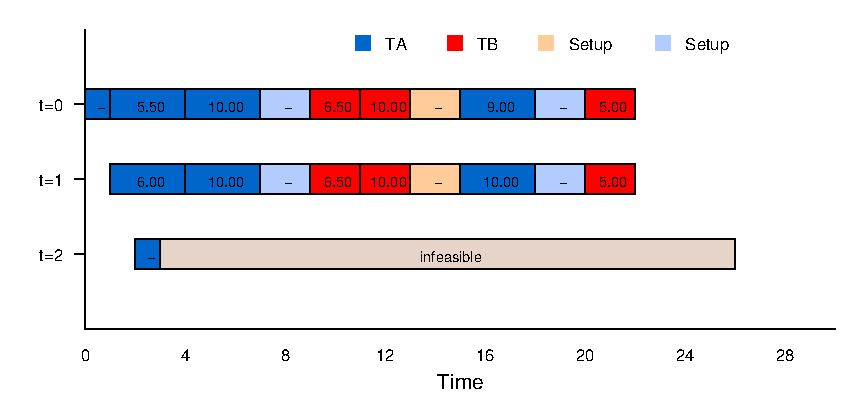
\includegraphics{scheduling/gantt_NT.pdf}
\caption{Rescheduling leads to infeasibility when no backorders are allowed}
\label{fig:scheduling:gantt_NT}
\end{center}
\end{figure}

\begin{alignat}{2}
\label{eq:scheduling:Periodic}
\mathbb{P}_P:& \min_{\bu,x(0)}{\sum_{t=0}^{N_P-1}
  \ell_E(x(t),u(t),d^{\text{nom}}(t))} &\nonumber \\ 
&\text{s.t.~} x(t+1) = Ax(t) + Bu(t)+B_dd^{\text{nom}}(t), &\qquad t = \set{0,1,\ldots,N-1}\nonumber\\
&\underline{b} \leq E_xx(t) + E_u u(t) \leq \bar{b},& \qquad t = \set{0,1,\ldots,N-1}  \\
& x(0) = x(N_p)& \nonumber
\end{alignat}

The Gantt chart for the periodic solution is shown in Figure
\ref{fig:scheduling:gantt_Periodic}. 

\begin{figure}
\begin{center}
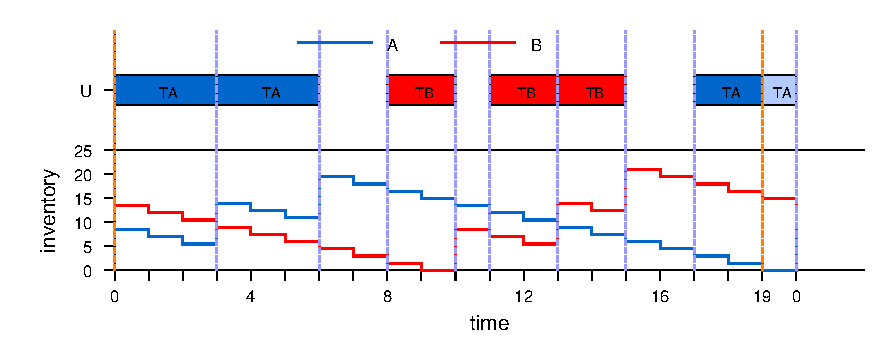
\includegraphics{scheduling/gantt_Periodic.pdf}
\caption{Periodic solution  for the example in the absence of disturbances}
\label{fig:scheduling:gantt_Periodic}
\end{center}
\end{figure}

We now illustrate the use of terminal constraints on the states of the
model which enable us to retain feasibility of the scheduling problem
as we roll the horizon forward. To do so, we use the cyclic schedule
found by optimization problem \eqref{eq:scheduling:Periodic}. Let the
solution of the \eqref{eq:scheduling:Periodic} be given as $(x_P^0(0),
u_P^0(0), u_P^0(1), \ldots, u_P^0(N_p-1))$. For this optimal periodic
solution, we can calculate the corresponding state-evolution using the
state evolution equation. Denote the states in this optimal periodic
state evolution as
$\set{x_P^0(0),x_P^0(1),\ldots,x_P^0(N_p-1)}$. Then the optimization problem
with terminal constraints $\mathbb{P}_N^T(x)$ can be written as:
\begin{alignat}{2}
\label{eq:scheduling:T}
\mathbb{P}_N^T(x):&
\min_{\bu}{\sum_{t=0}^{N-1}\ell_E(x(t),u(t),d^{\text{nom}}(t))}&
\nonumber \\ 
&\text{s.t.~} x(t+1) = Ax(t) + Bu(t)+B_dd^{\text{nom}}(t),& t = \set{0,1,\ldots,N-1} \nonumber\\
&\underline{b} \leq E_xx(t) + E_u u(t) \leq \bar{b},& t = \set{0,1,\ldots,N-1} \\
& x(0) = x &\nonumber\\
& x(N) \in \set{x_P^0(0),x_P^0(1),\ldots,x_P^0(N_p-1)}&\nonumber
\end{alignat}

In optimization problem $\mathbb{P}_N^T$, we enforce the condition
that the terminal state be one of the states in the optimal periodic
state evolution. Therefore, the solutions to \eqref{eq:scheduling:T}
contains long-term information. This is because, we terminate at a
state from which we can implement a periodic solution to respond to
nominal demands. The Gantt chart obtained by successive
re-optimization using problem \eqref{eq:scheduling:T} is shown in
Figure \ref{fig:scheduling:gantt_Terminal}. Due to design of the
optimization problem, we remain feasible at all times. Note that the
batch of $\text{TA}$ at $t=1$ was 8 tons, because of the information
regarding future demands contained in the terminal constraint. Figure
\ref{fig:scheduling:T_24_CL} shows the closed-loop solution over 24h.

\begin{figure}
\begin{center}
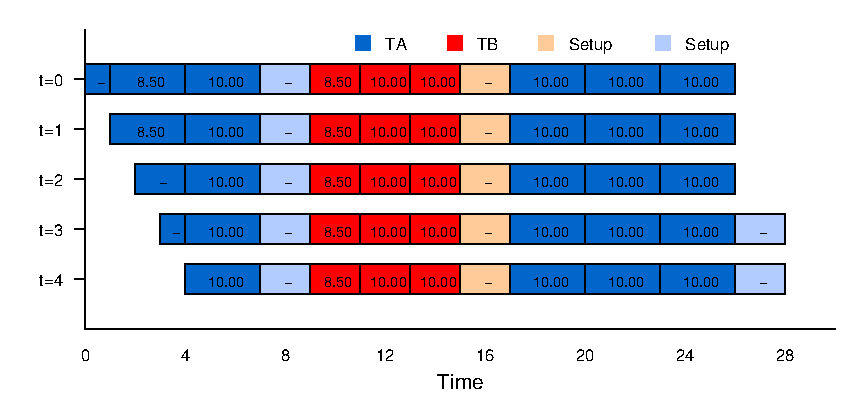
\includegraphics{scheduling/gantt_24.pdf}
\caption[Recursive feasibility with terminal constraints]{Solutions
  obtained by solving Problem \eqref{eq:scheduling:T} 
at $t=0,1,3$ and $4$. Addition of terminal constraints leads to
feasible problems. Compare the schedule at $t=0$ with
\ref{fig:scheduling:gantt_NT}. A larger batch of TA starts at $t=1$
and there are fewer changeovers, thus larger production.}
\label{fig:scheduling:gantt_Terminal}
\end{center}

\end{figure}
\begin{figure}

\begin{center}
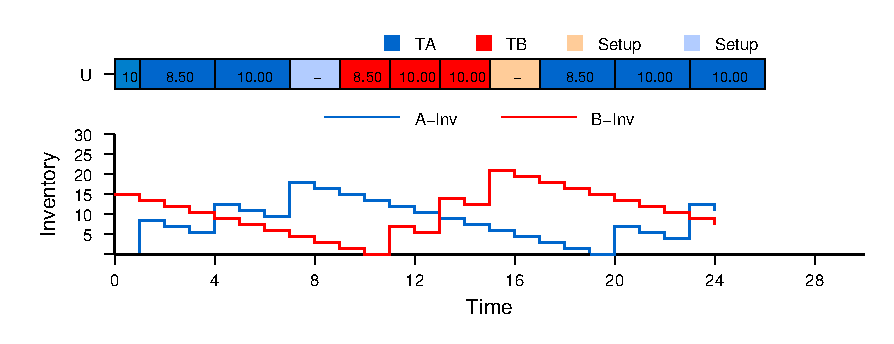
\includegraphics{scheduling/T_24_CL.pdf}
\caption{Closed-loop solution solving \eqref{eq:scheduling:T} with
  $N=24h$}
\label{fig:scheduling:T_24_CL}
\end{center}
\end{figure}

We can use terminal constraints to reduce the computational burden in
scheduling because, as shown in Figure \ref{fig:scheduling:gantt_12},
we can guarantee recursive feasibility using shorter prediction
horizons also. In Figure
\ref{fig:scheduling:gantt_12}, Problem \eqref{eq:scheduling:T} was
solved with $N=12$ and Figure \ref{fig:scheduling:T_12_CL} shows the closed-loop
solution over a horizon of 24h using a prediction horizon of $12h$.

 
\begin{figure}
\begin{center}
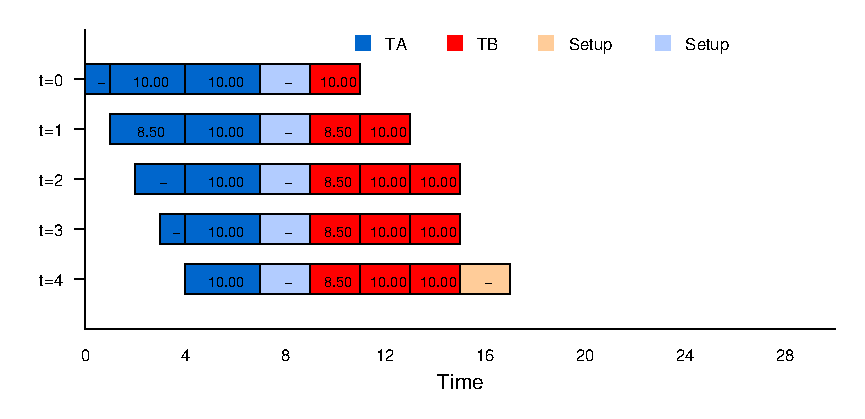
\includegraphics{scheduling/gantt_12.pdf}
\caption[Recursive feasibility with terminal constraints for
$N=12h$]{Solutions obtained by solving Problem \eqref{eq:scheduling:T} 
at $t=0,1,3$ and $4$. Recursive feasibility is maintained with proper
choice of terminal constraints}
\label{fig:scheduling:gantt_12}
\end{center}
\end{figure}
\begin{figure}

\begin{center}
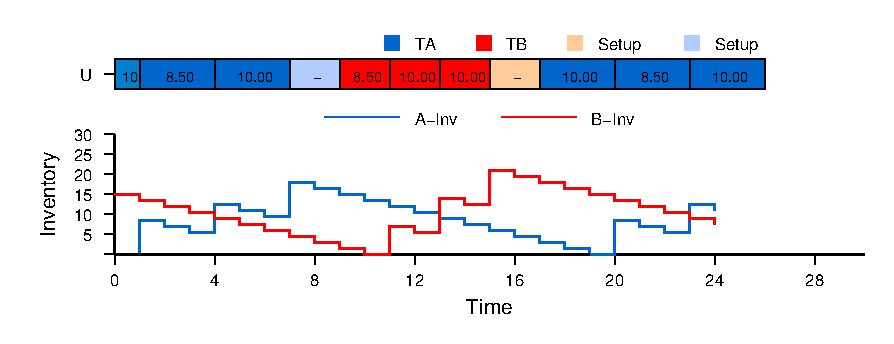
\includegraphics{scheduling/T_12_CL.pdf}
\caption{Closed-loop solution solving \eqref{eq:scheduling:T} with
  $N=12h$}
\label{fig:scheduling:T_12_CL}
\end{center}
\end{figure}

\subsection{Rescheduling}
In this section, we consider the same model as in Section
\ref{sec:scheduling:example:nominal}, but with backlogs. That is, we
introduce shipments $V_{k,t}$ and backlog $U_{k,t}$ with the new state
equations defined by \eqref{eq:scheduling:xbacklog} and
\eqref{eq:scheduling:backlog}. We enforce an economic penalty on
accumulating backlogs. 

The following disturbances are observed: (i) Production delay of 1h
at $t=6$, (ii) breakdown for 3h  from $t=10$ to $t=13$, (iii)
unloading error at $t=14$ (production of  B is 8ton instead of 10ton)
and, (iv) demand spike at $t=16$, with $\hat{\xi}_i = 0.5$, that is
the demand for both products were 2tons instead of the nominal demand
of 1.5 ton. Figures \ref{fig:scheduling:gantt_NT_disturbance} and
\ref{fig:scheduling:CL_NT_disturbance} shows the closed-loop
performance for an optimizer optimizing \eqref{eq:scheduling:NT}. We
can observe the rescheduling that occurs naturally using the rolling
horizon framework in Figure
\ref{fig:scheduling:gantt_NT_disturbance}. For example, the batch
sizes change between $t=6$ and $t=7$ and $t=14$ and $t=15$ after the
realization of disturbances. Finally, Figure
\ref{fig:scheduling:CL_T_disturbance} shows the closed-loop response
for the same disturbances, but when the optimizer was solving
\eqref{eq:scheduling:T}; that is, when we were enforcing terminal
cyclic constraints. We observe  inherent robustness of the
terminal constraint formulation as the backlogs accumulated are
lesser than the formulation without terminal constraints. 
\begin{figure}
\begin{center}
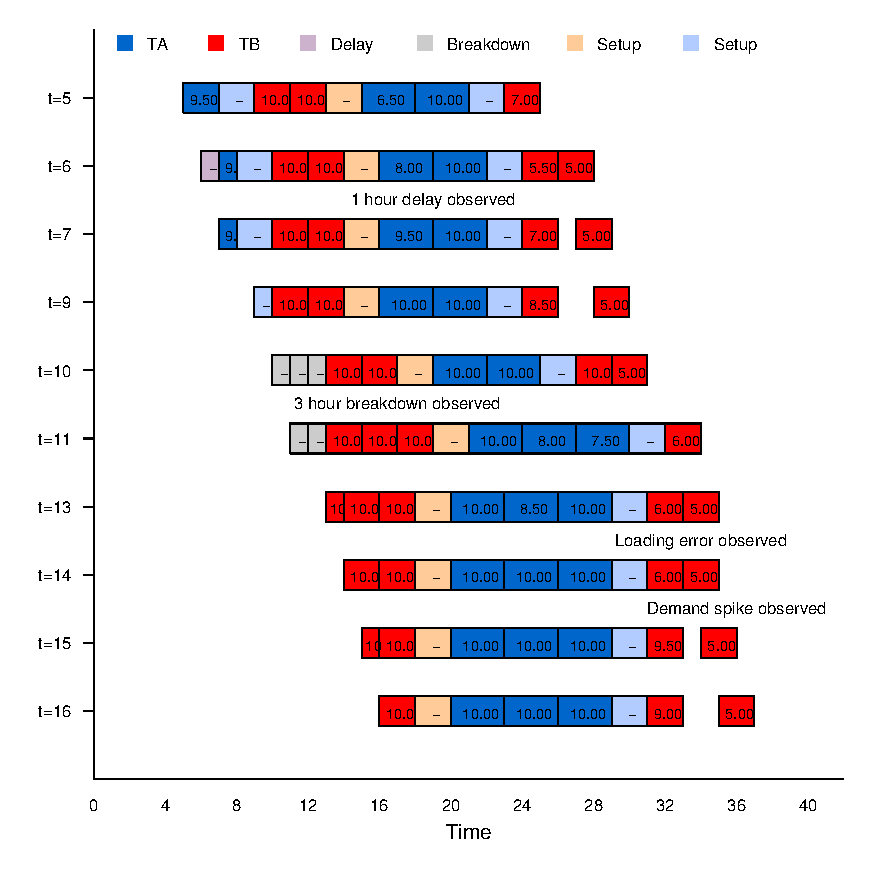
\includegraphics{scheduling/gantt_NT_disturbance.pdf}
\caption{Rescheduling in the presence of disturbances}
\label{fig:scheduling:gantt_NT_disturbance}
\end{center}
\end{figure}

\begin{figure}
\begin{center}
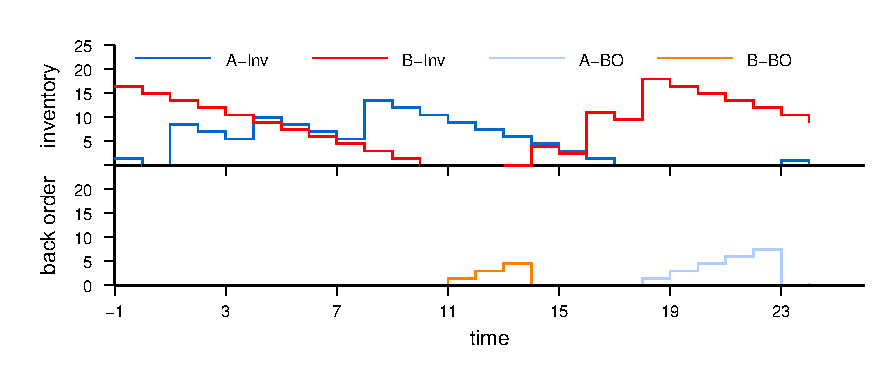
\includegraphics{scheduling/CL_NT_disturbance.pdf}
\caption[Closed-loop with disturbances]{Inventory (Inv) and Backorder(BO) profiles in the closed-loop
  in the presence of disturbances.}
\label{fig:scheduling:CL_NT_disturbance}
\end{center}
\end{figure}


\begin{figure}
\begin{center}
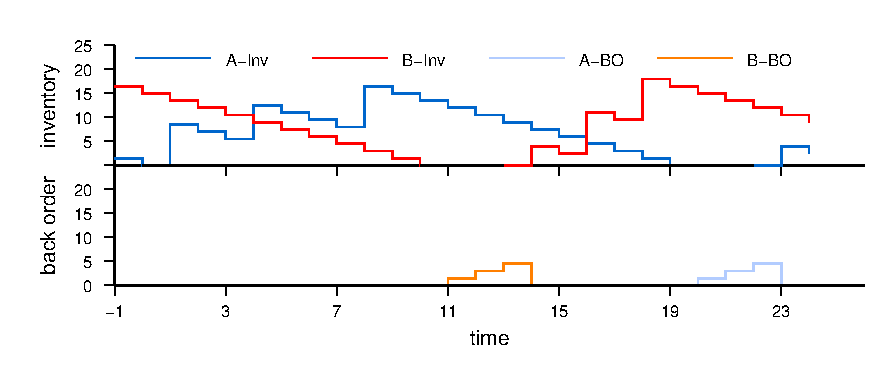
\includegraphics{scheduling/CL_T_disturbance.pdf}
\caption[Closed-loop for terminal constraint formulation with disturbances]{Inventory (Inv) and Backorder(BO) profiles in the closed-loop
  in the presence of disturbances. Compare with
  \ref{fig:scheduling:CL_NT_disturbance} to notice the inherent
  robustness of the terminal constraint formulation}
\label{fig:scheduling:CL_T_disturbance}
\end{center}
\end{figure}




\section{Discussion}
\subsection{Generality of the scheduling model\footnote{This text appears in Section 3.5.1 of \citet{subramanian:maravelias:rawlings:2012}}}

Most current approaches to reactive scheduling are based on scheduling
models that do not include disturbances explicitly. Thus, when an event
triggers rescheduling, an empirical procedure is followed to modify the
scheduling model so it (i) represents the new state of the system, and
(ii) accounts for the future impact of the disturbance. One advantage
of the state space model is that the same model can be directly used
for rescheduling. All events that can trigger rescheduling are modeled
via disturbance variables. Thus, for a resolve it is sufficient to fix
the appropriate disturbance variables, which can be readily calculated
from the observation at the current time. No empirical model
modifications are necessary.

\subsection{Stochastic vs. deterministic approaches\footnote{This text appears in Section 3.5.2 of \citet{subramanian:maravelias:rawlings:2012}}}

In this paper, we treat scheduling as an on-line problem; we optimize
to determine a single schedule based on current data and forecasts,
and as new information becomes available we re-optimize to determine,
again, a single solution. In each re-optimization, we solve a
deterministic problem- we do not account for the fact that some data
are subject to uncertainty that can be modeled. An alternative
approach is to model the uncertainty in the events that can trigger
rescheduling, and then generate a solution that takes into account
this information \citep{li:ierapetritou:2008b,sahinidis:2004}. The
obvious advantage of this so-called {\em{optimization under
    uncertainty}} approach is that, if the model is solved
effectively, then it can lead to better solutions. The disadvantage is
that most optimization under uncertainty methods are computationally
expensive, and thus cannot be used to address practical
problems. Robust optimization methods have been proposed to address
this shortcoming
\citep{ben-tal:nemirovski:2002,verderame:floudas:2009}; they rely on
solutions that is almost as hard as the deterministic problem, but
leads to solutions that are conservative. The advantage of the
control-inspired approach that we follow is that the deterministic
optimization problem can be solved more effectively, which has three
implications. First, it can lead to optimal (or near optimal)
solutions that are better (even when evaluated under uncertainty) than
the solution that can be obtained within the same time by a stochastic
programming approach. Second, it allows us to reschedule more
frequently, thus reacting faster to disturbances and thereby resulting
in better closed-loop solution. Third, it allows us to consider longer
scheduling horizons, which is critical and can often be more
important that accounting for uncertainty.

\subsection{Types of disturbances and uncertainties\footnote{This text appears in Section 3.5.3 of
  \citet{subramanian:maravelias:rawlings:2012}. Equation
  \eqref{eq:scheduling:discussion} has been modified to remain
  consistent with the notation used in this chapter}}

Interestingly, the types of disturbances we have discussed
correspond, when treated as stochastic parameters, to different types
of uncertainty. Shipment disturbances can be viewed as right-hand side
(RHS) uncertainty. Production and consumption disturbances can be
viewed as left-hand side (LHS) uncertainty, since they can be treated
as uncertainties in the $\beta_{ik} = \rho_{ik}\beta_i$ terms:

\begin{equation}
\label{eq:scheduling:discussion}
S_{k,t+1} = S_{k,t}+ \sum_{i \in
  \mathbb{I}^+}(\beta_{i}\bar{W}_{i,t}^{n}+\beta_{i,k,t}^P)\rho_{ik}
+\sum_{i \in
  \mathbb{I}^-}(\beta_{i}{W}_{i,t}+\beta_{i,k,t}^C)\rho_{ik} +
\zeta_{k,t} \qquad \forall k,t
\end{equation}

These are two types of uncertainty that have received the most
attention in stochastic optimization approaches to scheduling.

Task delays can also be treated as LHS uncertainty if the duration of
a task appears only as a LHS coefficient (in the case of fixed
processing times) or as a variable defined in terms of stochastic
parameters (in the case of variable processing
times). Precedence-based models or time-grid based models with
continuous modeling of time may result in stochastic optimization
problems which lead to LHS uncertainty. However, in discrete-time
formulations, the number of terms included in the summation in the LHS
of the assignment constraint depends on the duration of a task. Thus,
in this case, the treatment of task delays through the modeling of
processing times as stochastic parameters leads to a
{\emph{structural}} type of uncertainty.

Finally, unit breakdowns lead to structural uncertainty since the
constraints used to model resource constraints should be removed or
modified. Stochastic optimization approaches cannot be used to
effectively address this type of structural uncertainty because, in
addition to requiring on-the-fly reformulations of the scheduling
model, task delays and unit breakdowns lead to problems with either
{\emph{purely endogenous}} uncertainty or {\emph{exogenous uncertainty
    with endogenous observation}} \citep{colvin:maravelias:2008,colvin:maravelias:2010,goel:grossmann:2006}. For example, the
  probability and the timing of a unit breakdown depends on the
  utilization of the unit, which is determined by the decision
  maker. The proposed approach does not suffer from this limitation. 

\subsubsection{Reverse transformation and reoptimization\footnote{This text appears in Section 3.5.2 of \citet{subramanian:maravelias:rawlings:2012}}}

Since scheduling MIP models are computationally expensive, a potential
disadvantage of the proposed state space modeling framework is that it
leads to MIP models of larger size. For example. compared to its
counterpart model, $\mathbf{M}^{\text{SCH}}$, model
$\mathbf{M}^{\text{MPC}}$, has additional lifted variables (lifted
inputs $\bar{W}_{i,t}^{n}$) and
equations \eqref{eq:scheduling:liftedW}. However, model $\mathbf{M}^{\text{MPC}}$
is not significantly slower than $\mathbf{M}^{\text{SCH}}$. First we
note that the addition of disturbance variables in Equations
\eqref{eq:scheduling:finalSS} and
\eqref{eq:scheduling:breakdown_constraint} leads to changes in RHS
constant vector $b$, if the optimization model is written as
$\max_{}{\set{c'x: Ax \leq b. x \in \mathbf{X}}}$. In other words,
they do not increase the complexity of the model. Second, the lifting
equations can be used to project out variables after the state of the
system is updated using $\mathbf{M}^{\text{MPC}}$ and before
reoptimization is performed. Commercial MIP solvers perform this type
of preprocessing (variable elimination and constraint removal) automatically
\citep{atamturk:savelsbergh:2005}. Third, specific preprocessing
methods can be easily developed to transform the {\emph{current}}
$\mathbf{M}^{\text{MPC}}$ model (i.e. the model after the injection of
disturbances at $t$) back to a model in the form
$\mathbf{M}^{\text{SCH}}$. Perprocessing based on
$\mathbf{M}^{\text{MPC}}$ can also be used to automatically detect
what constraints should be removed or modified. For example. in the
case of a breakdown of unit $j=U$ from $t_1$ to $t_2$, the constraint
\eqref{eq:scheduling:breakdown_constraint} becomes:
\[ \sum_{i\in \mathbf{I}_j}W_{i,t} + \sum_{i \in
  \mathbf{I}_j}\sum_{n=1}^{\tau_i-1} \bar{W}_{i,t}^{n} \leq 0 \qquad
\forall t \in \set{t_1,\ldots,t_2-1}
\] 
which mathematically implies that all binary variables appearing in
the LHS should be fixed to zero and Equation
\eqref{eq:scheduling:breakdown_constraint} be removed from the model
for $j=U$ and $t\in \set{t_1,\ldots,t_2-1}$. Not surprisingly, this is
what one would do using logical arguments: if there is a breakdown in
an unit, then no tasks can be started on this unit (i.e., all binaries
are set to zero), and thus the corresponding assignment constraint can
be removed. Model $\mathbf{M}^{\text{MPC}}$ allows us to
systematically perform this type of reasoning. We note that our
preliminary computational experience confirms that
$\mathbf{M}^{\text{MPC}}$ is computationally comparable with model
$\mathbf{M}^{\text{SCH}}$. 


Finally, lifting the inputs offers
insights into generation of the models for rescheduling. As we saw,
the current state of the system includes past inputs from
$t-\max_i{\tau_i}$ to $t$. Hence, when reformulating original model
$M^{\text{SCH}}$, we have to fix the decisions made in the last
$\max_i{\tau_i}$ periods. This approach has been proposed in the past
\citep{sundaramoorthy:maravelias:2010}. The use of state space models
and input lifting formalizes this approach and makes it easy to write
rescheudling model for any disturbance. 

\subsection{MPC tools\footnote{This text appears in Section 6.1 of \citet{subramanian:maravelias:rawlings:2012}}}

The development of a state space model is a first step towards the use
of MPC theory and methods to address scheduling problems. It offers a
representation of scheduling problems with which the process control
community is familiar. Since scheduling is a dynamic problem and can
be viewed as a {\emph{production}} control problem, our hope is that
the proposed framework will enable MPC technology for scheduling
problems. 

Another outcome is that if facilitates the application of methods that
have been developed for hybrid dynamic systems consisting of both time
and event driven dynamics \citep{bemporad:morari:1999,
  heemels:schutter:bemporad:2001}. Control of such systems has been the
focus of many researchers in the past decade (see \citep{camacho:ramirez:limon:pena:alamo:2010} for a
review of MPC techniques for hybrid systems). At the same time,
studying this new class of problems can lead to the development of new
tools for hybrid system.

The state space model can also help to bridge the gap between
scheduling and control since it allows the formulation of the
integrated scheduling-control problem using a state space
model. Furthermore, the unified problem can be viewed as an economic
MPC problem in which the process economics (primarily determined by
the scheduling decisions) are directly optimized by the controller \citep{diehl:amrit:rawlings:2011}.

More importantly. it offers a natural framework for the development
of new scheduling algorithms based on MPC. As mentioned in Section
\ref{sec:scheduling:introduction}, scheduling is still thought of as
an open-loop problem, even though it is used in an iterative
manner. As a results, concepts such as stability,
recursive-feasibility, and closed-loop performance have received no
attention. In Section \ref{sec:scheduling:example}, we showed how
terminal constraints can be used to guarantee recursive feasibility.





%end chapter

\newcommand{\I}{\mathcal{I}}
\newcommand{\BO}{\textrm{BO}}
\newcommand{\IP}{\textrm{Ip}}
\newcommand{\UP}{\textrm{Up}}
\newcommand{\DN}{\textrm{Dn}}
\newcommand{\Inv}{\textrm{Iv}}
\newcommand{\Dem}{\textrm{Dm}}
\chapter{Distributed MPC for supply chain optimization}
\label{chap:sc}
We propose cooperative model predictive control for supply chains in
this chapter. 

In Section \ref{sec:sc:litreview}, we provide a brief review of the
different control theory based and distributed decision making
approaches to supply chain optimization and operation. In section
\ref{sec:sc:modeling}, we describe the dynamic modeling of supply
chains. In section \ref{sec:sc:supplychain_example}. we implement
cooperative MPC on a 
single-product, two-echelon supply chain. Finally, we summarize our
results  in Section \ref{sec:sc:discussion}.

\section{Introduction\footnote{ The text in this section appears in Section 1 of
\citet{subramanian:rawlings:maravelias:2012}.}}
\label{sec:sc:intro}
The supply chain is a system comprising organizations, decision
makers, and  technology decision policies that is responsible for
transforming raw materials into finished products that are delivered
to end customers. 
As expanded upon later in this paper,
the supply chain is traditionally characterized
by counter-current flows of information and material. Material
flows from the raw material suppliers through the production and
distribution facilities to the end customers, while information, in
the form of demands and orders, flows from the end customers upstream
to the suppliers \citep{backx:bosgra:marquardt:1998,beamon:1998}.


The decisions for supply chain management can be broadly classified
into three categories: strategic, tactical and operational. The
strategic decisions   
are the long term planning decisions that may include, among others,
where to locate production facilities and warehouses,
and in which technologies to invest. On a medium time range,
tactical decisions include selecting supply chain partners such as raw
material suppliers, transportation companies, etc. The operational
decisions are the short term decisions, which are related to optimally
operating the supply chain. These decisions include planning and
scheduling in the production facilities, and distribution decisions
such as inventory management, ordering and shipping policies,
etc. \citep{shah:2005,ganeshan:harrison:1995}. 

\citet{shapiro:2004} lists the challenges in enlarging the scope of
strategic planning in supply chains. Among the listed challenges are
integrating manufacturing, purchase and sales decisions, multiperiod
analysis and optimizing the overall supply chain profits. \citet{
stadtler:2005} is an excellent overview paper about advanced planning
in supply chains. The authors emphasize  linking
organizational units to improve competitiveness of the supply
chain. However, from an operational viewpoint, they focus on advanced
planning systems (APS) that uses  information and
communication technology to coordinate all the flows (material,
information, financial) in the supply chain to best improve customer
satisfaction.

The combined strategic and operational planning is a challenging
optimization problem, but researchers have made efforts to solve it;
see, for instance,
\citep{sabri:beamon:2000,tsiakis:shah:pantelides:2001,you:grossmann:2008}. 
The optimization problems formulated for combined strategic and
operational planning typically involve selecting a supply chain
network from a family of networks or a network
superstructure. Recent developments in combined strategic and
operational planning, including handling of uncertainties and
multi-objective formulations, are described in the review paper
\citep{papageorgiou:2009}.  

At the operational level of the supply chain, the need for
simultaneous decision making  at the manufacturing and the
distribution sites to operate a \textit{coordinated} supply chain has
been recognized. The focus of this chapter is on methods to achieve such
simultaneous decisions. This simultaneous decision making is also
known as enterprise wide optimization \citep{grossmann:2005}.

Modern supply chains operate over multiple locations and products, and
are highly interconnected. In a competitive economy, neglecting these
interactions may result in lower profits. A central coordinator who
controls the supply chain can account for these interactions and
provide optimal operation. However, centralized coordination may not
always be practical for a supply chain as (i) different nodes may
belong to different firms, (ii) there may be a conflict of objectives
among nodes (iii) information sharing may not be  perfect and (iv) a
centralized decision maker is the most vital cog in a supply
chain, and its failure may be catastrophic for the supply
chain. Therefore, distributed coordination structures for supply chain
operation is needed.

We focus  on tailoring model predictive control (MPC) as a general
purpose method for optimal supply chain operation. 
Model predictive control uses a dynamic model of the system
to predict future outcomes and solves a constrained optimization
problem over the predicted outcomes to find the best operational
decisions. Therefore, it is well suited as a basis for supply chain
operation because it makes full use of the dynamic model and knowledge
of the interactions between the various nodes to predict and optimize
an overall supply chain objective function.

We propose cooperative MPC as a tool for coordinating supply chains as
it retains 
the same structure as traditional supply chains wherein each node
makes its own local decisions, but instead of optimizing the local
objective functions, the nodes optimize the overall supply chain
objective function.




\section{Literature survey\footnote{The text in this section appears in Section 2 of
\citet{subramanian:rawlings:maravelias:2012}}}
\label{sec:sc:litreview}
A well defined supply chain optimization model requires a detailed
dynamic description of the supply chain and an objective function that
captures all the essential costs and trade-offs in the supply chain.
\citet{beamon:1998} classifies supply chain modeling 
in four broad categories: Deterministic models where all the
parameters are known, stochastic models with at least one unknown
parameter (typically demands) that follows a known probability
distribution, economic game theory based models, and simulation based
models. As pointed out in
\citep{sarimevis:patrinos:tarantilis:kiranoudis:2008}, a majority of
these models are steady-state models based on average performance, and
hence are unsuitable for dynamic analysis. In the review of dynamic
models for supply chains, 
\citet{riddalls:bennett:tipi:2000} classify the models as continuous
time models, discrete time models, discrete event simulations, and
operations research (OR) based models.  

The pioneering work of
``industrial dynamics'' awakened the 
control community's interest in supply chain optimization. The
industrial dynamics models are the continuous (and discrete) time
dynamic models mentioned in \citep{angerhofer:angelides:2000}.
Industrial dynamics captures the dynamics of the supply chains using
differential (or difference) equations, and therefore, control theory is a
natural choice to study supply chain dynamics. In their simplest form,
these models capture inventory  dynamics based on the shipments and
orders leaving the node 
\begin{equation*}
\Inv_i(k) = \Inv_i(k-1) - \sum_{j \in \DN(i)}S_{ij}(k) + \sum_{j \in
  \UP(i)}S_{ji}(k-\tau_{ji}) 
\end{equation*}
in which $\Inv_i(k)$ is the inventory in node $i \in \I$ at
discrete time $k$, $\DN(i)$ is the set of nodes to which node $i$
ships material and $\UP(i)$ is the set of nodes from which node $i$
receives material. The shipment delay between  nodes $i$ and $j$ is
denoted $\tau_{ij}$, and $S_{ij}$ is the amount shipped by node $i$ to
node $j$. 

In order to compare different methods of supply chain operation,
supply chain performance has to be quantified.  
\citet{beamon:1999,beamon:1998} classify the performance measures in a
supply chain as quantitative measures like cost minimization, profit
maximization, customer response time minimization and, qualitative
measures like customer satisfaction, flexibility etc. An important
performance measure that   
supply chain operation  strives to reduce is the \textit{bullwhip
  effect}, which is defined as the amplification of demand
fluctuations as one moves upstream in the supply chain. It has been
observed that the orders placed by a node to its upstream nodes
amplify (with respect to the customer demand) as one moves towards
the supplier in a supply chain. This effect increases the cost of
operating the supply chain. It has been estimated that a potential 
30 billion dollar opportunity exists in streamlining the inefficiencies of
the grocery supply chain, which has more than 100 days of inventory
supply at various nodes in its supply chain
\citep{lee:padmanabhan:whang:1997,lee:padmanabhan:whang:1997b}. Among
the reasons cited for 
the bullwhip effect is information distortion as one moves
upstream in the supply chain. Information sharing has been shown to
alleviate the bullwhip effect and is part of industrial practice such as
vendor managed inventory (VMI), etc. The other reasons often cited for
the bullwhip effect are: (i) the misunderstanding of feedback, which occurs
because the nodes do not understand the dynamics of the supply chain,
and (ii) the use of local optimization without global vision, in which each
node tries to maximize its local profit without accounting for the effects
of its decisions on the other nodes in the supply chain
\citep{moyaux:chaib-draa:damours:2007}. Centralized operation of
supply chains is best suited to mitigate bullwhip effect, as it has
exact knowledge  of the dynamics and complete information. 
 

\subsection*{Classical control theory}
The earliest applications of control theory to supply chains involved
studying the transfer functions and developing single input single
output (SISO) controllers for
tracking inventory to its targets. Frequency domain analysis was used
to analyze and evaluate alternative supply chain
designs. In classical control approaches to controlling supply chain,
the nodes were analyzed as linear systems using Laplace and
$Z$-transforms. In the work of \citet{Towill:1982}, a block diagram
based 
approach to modeling a node was proposed. The single product node
consisted of two integrators to capture the dynamics of inventory and
backorders, while the order rate was the
manipulated variable. The disturbance to the system, market demand,
was incorporated in a feed-forward manner in the model. Time delays were
also incorporated in the model. A feedback control law was
proposed for controlling the inventory deviations from a target
inventory. By varying some of these  parameters like delay,
controller gain etc., a family of models for a single
node called as the input-output based production control system
(IOBPCS) can be studied 
\citep{lalwani:disney:towill:2006}. The feedback law, in its simplest
form, takes the form of an order-up-to policy, that is order up-to the
inventory target, if the current inventory is below its target. This
policy can be viewed as a saturated proportional controller, although
other forms of the controller can also be studied. Upon having a
control policy and after defining other system details like
delays, forecast smoothing etc, the transfer function of the node can
be derived and analyzed
\citep{dejonckheere:disney:lambrecht:towill:2003}. 
\citet{white:1999,wikner:naim:towill:1992} 
developed a PID controller without feed-forward forecasting for the
node. A review of stability analysis for the IOBPCS family of models
is presented in \citet{disney:towill:warburton:2006}.

Classical control theory has also been studied for controlling the
dynamics of the entire supply chain as
well. \citet{grubbstrom:tang:2000} provides a review of the
input-output modeling of supply chains and its analysis using Laplace
transforms. Input-output modeling is the matrix form description of
the supply chain
dynamics. \citet{burns:sivazlian:1978,wikner:towill:naim:1991}
analyzed 
multiechelon supply chains using the block diagram based
approach. They analyzed the effect of ordering policies, delays and
information availability at the nodes to analyze the supply chain
response and bullwhip effect. \citet{burns:sivazlian:1978} used
$Z$-transforms in their approach and found that information distortion
led to bullwhip effect. \citet{wikner:towill:naim:1991} found out that
information sharing and echelon inventory policies (in which each
echelon considers inventory in all the nodes downstream to it) can
mitigate bullwhip effect.
\citet{perealopez:grossmann:ydstie:tahmassebi:2001,
perealopez:grossmann:ydstie:tahmassebi:2000b}
have developed a continuous time model to describe a supply chain. The
model is similar to deterministic supply chain models but uses
differential equations to track dynamics. They simulated the model
using a heuristic shipping policy and studied the closed-loop supply
chain under three different proportional controllers for placing
orders. They developed controllers to track inventory, backorder or a
combination of both. The objective of the
paper was to demonstrate that the model was capable of capturing the
dynamics. Hence, they did not suggest any tuning methods for the
controllers.  \citet{lin:wong:jang:shieh:chu:2004} presented an
approach to analyze the closed-loop stability of a supply chain and an
approach for controller synthesis using a transfer function 
approach. The controller policy and shipping policy were similar to
the \citet{perealopez:grossmann:ydstie:tahmassebi:2001}
paper. They analyzed stability considering three extreme closed-loop
scenarios: (i) high inventories and infinite replenishment from
upstream nodes (infinite production),(ii) a low inventory and infinite
replenishment from upstream nodes and (iii) limited
production/supply. The effect of controller gains on the bullwhip
effect was also analyzed. The authors proposed a controller tuning
criterion based on frequency domain analysis of the $Z$-transfer
functions. \citet{venkateswaran:son:2005} also studied the supply
chain response using $Z$-transform and derived stability conditions
for the supply chain. \citet{hoberg:bradley:thonemann:2007} applied
linear control theory on a two-echelon supply chain and concluded that
order-up-to policy based on inventory on hand can lead to
instabilities. They found that the use of an echelon policy
provides the best
performance. \citet{dejonckheere:disney:lambrecht:towill:2004} studied
information enrichment where in, each node receives the final customer
demand as well as the orders placed by its downstream nodes, using a
linear control theory based approach and concluded that information
enrichment is beneficial to the supply
chain. \citet{papanagnou:halikias:2008}  used a proportional
controller to place orders and analyzed the bullwhip effect by
estimating the state covariance matrix, for a supply chain responding
to a random demand (modeled as a white noise) at the retailer node.


\citet{sarimevis:patrinos:tarantilis:kiranoudis:2008,ortega:lin:2004}
provide extensive reviews of classical control approaches to supply
chain design and operation.

\subsection*{Stochastic optimal control}
Stochastic optimal control has been used to obtain ordering policies
that minimize the expected costs of a node responding to random
demands. We assume that the probability distribution of the demand is given.
 In its simplest form, the inventory control problem can be formulated
 as a dynamic optimization problem. The order-up-to policy is one such
 policy that is obtained by solving the dynamic optimization
 problem. The single node inventory control problem can be cast as a
 Markov decision problem. See \citet{puterman:2005} for details on
 setting up the problem and algorithms. 
The order-up-to policy is optimal for independent and identically
distributed demands as shown in the seminal paper by
\citet{clark:scarf:1960}. 
 By considering set-up costs, it can be shown that the $(\sigma,\Sigma),\sigma<\Sigma$
 policy, in which the node orders $\Sigma-\Inv$ whenever the inventory
 $\Inv$ falls below $\sigma$, is the optimal policy for an infinite horizon
 problem; see for instance
 \citep{veinott:1966,iglehart:1963,federgruen:zipkin:1984}. Optimality
 of similar policies have been shown for Markovian demands
 \citep{song:zipkin:1993,sethi:cheng:1997}, compound Poisson and
 diffusion demands \citep{bensoussan:liu:sethi:2006}, etc. 
 These results, derived for a single inventory holding
facility, have been extended to multiechelon systems,
\citep{federgruen:1993, shang:song:2003, dong:lee:2003,
  gallego:ozer:2005,chen:song:2001}and  capacitated
systems;
\citep{levi:roundy:shmoys:truong:2008,federgruen:zipkin:1986,federgruen:zipkin:1986b},
to better capture the dynamics of modern supply
chains. \citet{chen:ryan:simchi-levi:2000,chen:ryan:simchi-levi:2000b}
quantify the bullwhip effect for order-up-to policy under exponential
smoothing and moving average forecasts. We refer the readers to the
books by \citet{zipkin:2000} and \citet{axsater:2006} for more
details. 


\subsection*{Distributed decision making in supply chains}
Supply chain decisions have traditionally been made by managers at
each node. From a decentralized operation perspective, supply chains
can be analyzed using the tools of game theory.
In decentralized decision making, the payoff (profits) for each node
depends not only on its decisions, but also on the decisions made by
the other nodes. Therefore, supply chain
operations can be viewed as a strategic game between the various
nodes. Game theory based analysis can be further classified into
noncooperative and cooperative game theory.

In noncooperative game theory, each node simultaneously makes
decisions and then the payoff is obtained. Such games are
characterized by the Nash equilibrium that is the set of game
outcomes for which no node has a unilateral incentive to move away
from the outcome. At the Nash Equilibrium, no node can
increase its payoff by changing its decision while the
choices made by the other nodes remain the same. This result is
attributed to Nash in his seminal paper \citep{nash:1951}. Related to
Nash equilibrium is the Stackelberg equilibrium attributed to the
mathematician von Stackelberg. In a Stackelberg game the nodes 
make their decisions sequentially. We refer the reader to the
excellent text by \citet{ basar:olsder:1999} for detailed analysis into
game theory tools and
methods. \citet{leng:parlar:2005,cachon:netessine:2006} provide
excellent reviews of game theoretic methods applied to supply 
chains.


If the nodes make the supply chain optimal decision in a
noncooperative game, then the supply chain is said to be coordinated
\citep{cachon:zipkin:1999}. 
One of the methods to coordinate supply chains is to modify the 
interactions between the nodes of the supply chain (for example, by
adjusting contracts) so that each  node, optimizing its
local objective, makes the globally optimal decision. For example, a
two node newsvendor type supply chain can be coordinated using
buy-back contracts. A two node newsvendor supply chain consists of a
retailer and a supplier. The retailer faces a random demand with a
known probability distribution at each period. In order to respond to
this demand, the retailer buys product from the supplier at the
beginning of the period. The supplier is assumed to ship products
instantaneously. In the buy-back contract, the supplier agrees
to buy back unsold stock at the end of the season from the
retailer. The buy-back contract 
transfers  some of the risk of maintaining inventory to the supplier and
divides the supply chain optimal profit (the centralized profit) among
the partners. In contrast, the performance of  the wholesale (price
only) contract, in which the 
supplier supplies product at a wholesale price to the retailer,
can be arbitrarily poor. Under wholesale contract, the retailer takes all the risk
of excess inventory and orders
safely\citep{cachon:2003,cachon:zipkin:1999}. \citet{perakis:roels:2007}
quantified the inefficiencies in the supply chain (the ratio of the
decentralized supply chain profits to that of the centralized supply
chain profits) for the price only or wholesale
contracts. \citet{moses:seshadri:2000} showed that a  two-echelon supply
chain can be coordinated only if the manufacturer agrees to share a
fraction of the holding costs of the retailer's safety
stock. \citet{golany:rothblum:2006} also studied linear
reward/penalty as a contract modification to induce coordination in
the supply chain. \citet{li:wang:2007} provide a survey of the
various coordinating mechanisms. \citet{axsater:2001} studied the
Stackelberg game in the supply chain. \citet{axsater:2001} assumed that the
manufacturer is the leader in the Stackelberg game. The manufacturer
minimized the system-wide costs and declared its policies to the
retailers. The retailers  then optimized a modified cost function that
considers the policies of the manufacturer. They implemented an
iterative optimization algorithm such that the policies at every
iterate was better than the initial policy. The authors also noted
that the iterations 
may not converge to the centralized solution.
 

On the other hand, cooperative game theory is a branch of game theory
that studies the benefits of coalitions. A coalition between nodes
is formed when the nodes cooperate. These studies allocate payoffs to
various coalitions and these payoffs are analyzed via different
techniques like Shapley value \citep{shapley:1997} or nucleolus
\citep{schmeidler:1969}. \citet{raghunathan:2003} studied incentives
for nodes to form information sharing
partnerships. \citet{leng:parlar:2009}  studied different
coalitions in a three-echelon supply chain. For example, if the
manufacturer and distribution center form a coalition, then it is
assumed that the orders placed by the retailer are known to both the
nodes. Under the grand coalition, the final customer demand is shared
among all the three nodes.  \citet{leng:parlar:2009} defined the
payoff of a coalition as 
the cost savings obtained when  extra information due to the
coalition is available to the nodes. Using the
payoff of all the possible coalitions, they studied the stability of
different coalitions.  The authors  noticed that the bullwhip effect
is reduced when the 
manufacturer and distribution center formed a
coalition. \citet{bartholdi:ziya:2005} studied a two-echelon supply chain
in which a manufacturer supplies to multiple retailers. They used the
concepts of cooperative game theory to find profit allocation rules
after cooperation. Since the value allocation was in the core of the
cooperative game, it ensured that none of the participants in the
coalition have incentive to leave.  
\citet{nagarajan:sosic:2008} provide a comprehensive survey of
cooperative game theory applications to supply chains. 


\subsection*{MPC for supply chains}
\citet{perealopez:ydstie:grossmann:2003} developed a detailed
multi-product model including time delays and a mixed integer model
for the manufacturing facility. They modeled the shipment rates with a
``best I can do'' policy that satisfies all the accumulated orders at
a given time if stocks are available; otherwise it ships all of its
available stock. This  model was used for supply chain
control using MPC maximize profit. They considered three cases in
their implementation: a 
centralized case, and two other cases that they termed
``decentralized'' control. In one decentralized control scheme, they
optimized the mixed integer production facility while operating the
supply chain under a nominal control policy (like a proportional
controller for the orders). In the other decentralized control
scheme, they optimized only the orders in the supply chain subject to
a nominal production schedule. The authors advocated the use of
``centralized MPC''. \citet{mestan:turkay:arkun:2006} developed a
supply chain model using a 
hybrid systems approach and implemented  centralized,
decentralized, and noncooperative MPC as described in
\citep{rawlings:stewart:2008}. They compared customer satisfaction and
supply chain profit for the centralized and decentralized
MPC. The objective functions were chosen such that the retailer
objective of maximizing customer satisfaction was in conflict with the
objective of other nodes. Decentralized MPC had the highest customer satisfaction metric
but the supply chain operated at a loss. The bullwhip effect was high in the decentralized approach. In
centralized MPC, the supply chain found the trade-off between
maximizing customer satisfaction  and minimizing overall supply chain 
costs. The  centralized approach showed a small bullwhip effect because all the shipment and
order rates were determined by a central policy. The authors also
noted that the performance of noncooperative MPC was much better than
the performance of decentralized MPC.  \citet{dunbar:desa:2007a} solved a three-echelon, one-product supply
chain using a noncooperative MPC.  They developed a bidirectionally coupled model, by considering two
types of delay: pipeline delay or the transportation delay and
a first order material delay to quantify delays in clearing
backlogs.  The algorithm was found to be better than a nominal control
policy. They also observed  that the ordering policy was not very
aggressive, indicating  that the bullwhip effect may be
mitigated by distributed MPC. \citet{seferlis:giannelos:2004} presented a two-layer MPC strategy
for multiechelon supply chains. They used MPC to find shipments and
orders placed to other nodes, subject to a total order constraint. 
The total orders placed was the manipulated variable of a PID
controller to track inventory. The authors suggest that the performance can be improved by better tuning
the PID controller and suggest a bi-level optimization problem in
which the PID controller is replaced with an optimization-based
controller.  \citet{kempf:2004} and \citet{braun:rivera:carlyle:kempf:2002}  developed a
model predictive control framework for the supply chain in the semiconductor
industry. They developed models that are specific to the semiconductor
industry. \citet{braun:rivera:carlyle:kempf:2002}
implemented decentralized MPC and studied the control performance
under plant model mismatch.  \citet{kempf:2004}  described a two-loop optimization technique for
the supply chain optimization problem.  The coarse first loop
optimizer is used to generate the inventory and order setpoints
(reference trajectories), while the fine inner loop MPC is used to
track these setpoints. \citet{bose:pekny:2000} also used an MPC
framework. They focused on forecasting the demand signal  and
studied the sensitivity of the MPC framework to fluctuations in the
demand signal. \citet{Maestre:Pena:Camacho:2009} proposed a
cooperative MPC algorithm for a two-layer supply chain. In their 
formulation, each node minimized its local objective function, not
only over its own decision space, but also over the decision spaces of
the other nodes. Based on the multiple optimal objective function
values (one for each node), the algorithm determined a consensus
input. The drawback of the approach is that it is not scalable for
large supply chains with multiple
nodes. \citet{bemporad:cairano:giorgetti:2005} showed the applications
of hybrid 
MPC \citep{bemporad:morari:1999} on a centralized supply chain management
problem. \citet{li:marlin:2009} implemented robust MPC using an
economic objective function on a multiechelon 
supply chain.

In the following section, we show that the supply chain can be modeled
as a system of integrators. 

\section{Dynamic modeling of the supply chain\footnote{ This section has been modified from Section 3 of
\citet{subramanian:rawlings:maravelias:2012} to account for multiple
products in the supply chain. Equation \eqref{eq:sc:backorderbalance} has
been modified to track backorders for each downstream node separately.}}
\label{sec:sc:modeling}
A dynamic model is the heart of any feedback control algorithm. While
developing a dynamic model of a supply chain, the components of a
supply chain (like the production facility, distributor, retailer
etc.) are called as nodes. The supply chain network is the vertices or
arcs, which depict the connections between the various nodes. We
assume that the network is fixed and given to us. 
We denote the set of nodes by $\I$. The nodes to which a particular
node supplies material are called its 
downstream nodes, while the nodes from which a particular node obtains
material are called its upstream nodes.  The set of products handled
in the supply chain is given by 
$\mathcal{P}$. For a particular node $i \in \I$, the set
$\mathcal{P}(i)$ denotes the products handled by that node.
For each node $i \in
\I$, and each product $p \in \mathcal{P}(i)$ we define the set $\UP(i,p)$ as the set of all nodes $j \in
\I$ that are connected by an arc with $i$ and  are
upstream to node $i$. These nodes supply product $p$ to node $i$.
Similarly, we define the set of downstream nodes 
to $i$ for products $p$ as $\DN(i,p)$. For each arc in the the supply
chain, material flows downstream and orders (or information) flows
upstream.
The supply chain in the form of nodes and arcs is shown in
Figure \ref{fig:sc:Nodes_and_Arcs}.
\begin{figure}[h]
 \centering
 {\resizebox{0.75\textwidth}{!}{\begin{picture}(0,0)%
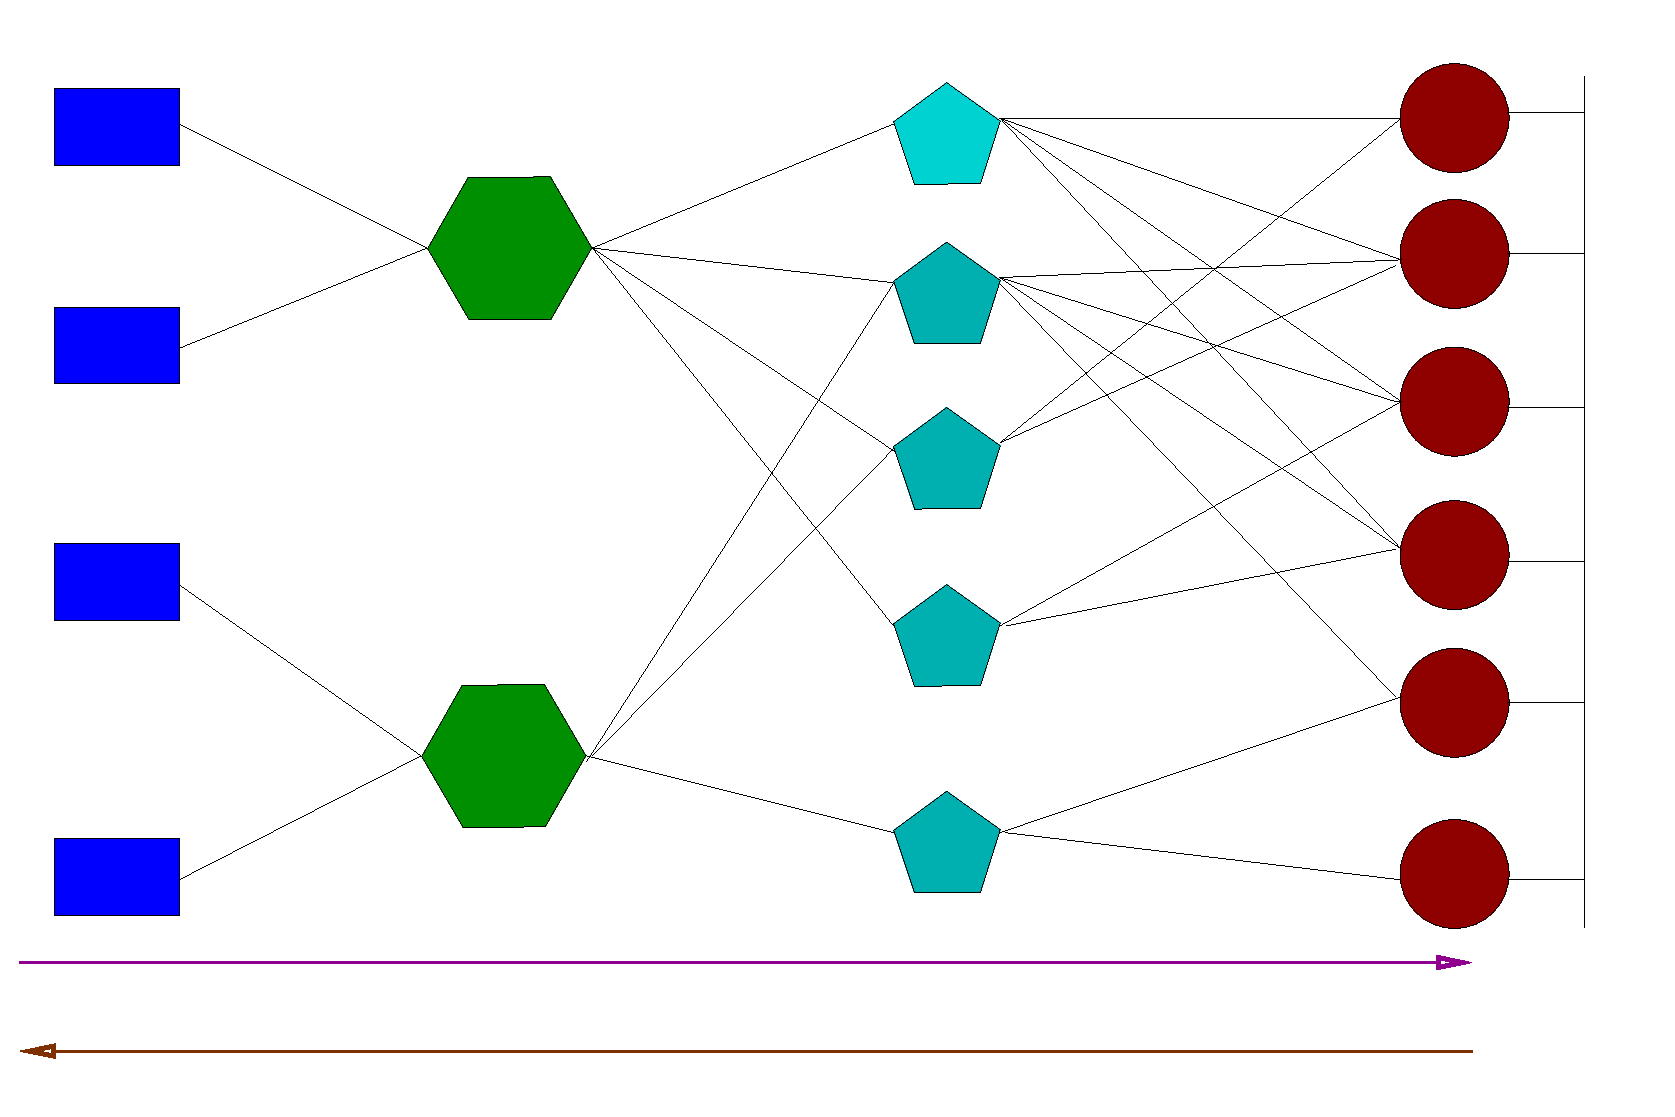
\includegraphics{sc/nodes1_color}%
\end{picture}%
\setlength{\unitlength}{4144sp}%
%
\begingroup\makeatletter\ifx\SetFigFont\undefined%
\gdef\SetFigFont#1#2#3#4#5{%
  \reset@font\fontsize{#1}{#2pt}%
  \fontfamily{#3}\fontseries{#4}\fontshape{#5}%
  \selectfont}%
\fi\endgroup%
\begin{picture}(12502,8244)(744,-8131)
\put(13231,-2626){\rotatebox{90.0}{\makebox(0,0)[rb]{\smash{{\SetFigFont{14}{16.8}{\rmdefault}{\mddefault}{\updefault}{\color[rgb]{0,0,0}CUSTOMERS}%
}}}}}
\put(9091,-7351){\makebox(0,0)[lb]{\smash{{\SetFigFont{17}{20.4}{\familydefault}{\mddefault}{\updefault}{\color[rgb]{.56,0,.56}Product Flow}%
}}}}
\put(946,-106){\makebox(0,0)[lb]{\smash{{\SetFigFont{17}{20.4}{\familydefault}{\mddefault}{\updefault}{\color[rgb]{0,0,1}Suppliers}%
}}}}
\put(7156,-106){\makebox(0,0)[lb]{\smash{{\SetFigFont{17}{20.4}{\familydefault}{\mddefault}{\updefault}{\color[rgb]{0,.69,.69}Distibution}%
}}}}
\put(7381,-331){\makebox(0,0)[lb]{\smash{{\SetFigFont{17}{20.4}{\familydefault}{\mddefault}{\updefault}{\color[rgb]{0,.69,.69}Centers}%
}}}}
\put(3826,-151){\makebox(0,0)[lb]{\smash{{\SetFigFont{17}{20.4}{\familydefault}{\mddefault}{\updefault}{\color[rgb]{0,.56,0}Production }%
}}}}
\put(4051,-511){\makebox(0,0)[lb]{\smash{{\SetFigFont{17}{20.4}{\familydefault}{\mddefault}{\updefault}{\color[rgb]{0,.56,0}Facility}%
}}}}
\put(11161,-106){\makebox(0,0)[lb]{\smash{{\SetFigFont{17}{20.4}{\familydefault}{\mddefault}{\updefault}{\color[rgb]{.56,0,0}Retailers}%
}}}}
\put(1396,-8116){\makebox(0,0)[lb]{\smash{{\SetFigFont{17}{20.4}{\familydefault}{\mddefault}{\updefault}{\color[rgb]{.5,.17,0}Information Flow}%
}}}}
\end{picture}%
}}
\caption{Supply chain as nodes and arcs.}
 \label{fig:sc:Nodes_and_Arcs}
\end{figure}

From a classical chemical engineering perspective, each node can be
modeled as two tanks, the inventory tank and the backorder tank. 
 The flows out of the inventory tank are the shipments
to the downstream nodes and the shipments from the upstream nodes make
up the flow into the inventory tank. The flows out of the backorder
tank are the shipments to the downstream nodes, which 
alternatively can be viewed as the orders that have been met; the
flows into the backorder tank are the orders arriving at the
node. For nodes that handle multiple products, we have as many
inventory and backorder tanks as the number of product handled by
the node.  Figure
\ref{fig:sc:nodemodel} depicts the `tanks' model of a node in the supply
chain handling a single product.
 \begin{figure}[h]
\centering
{\resizebox{0.75\textwidth}{!}{\begin{picture}(0,0)%
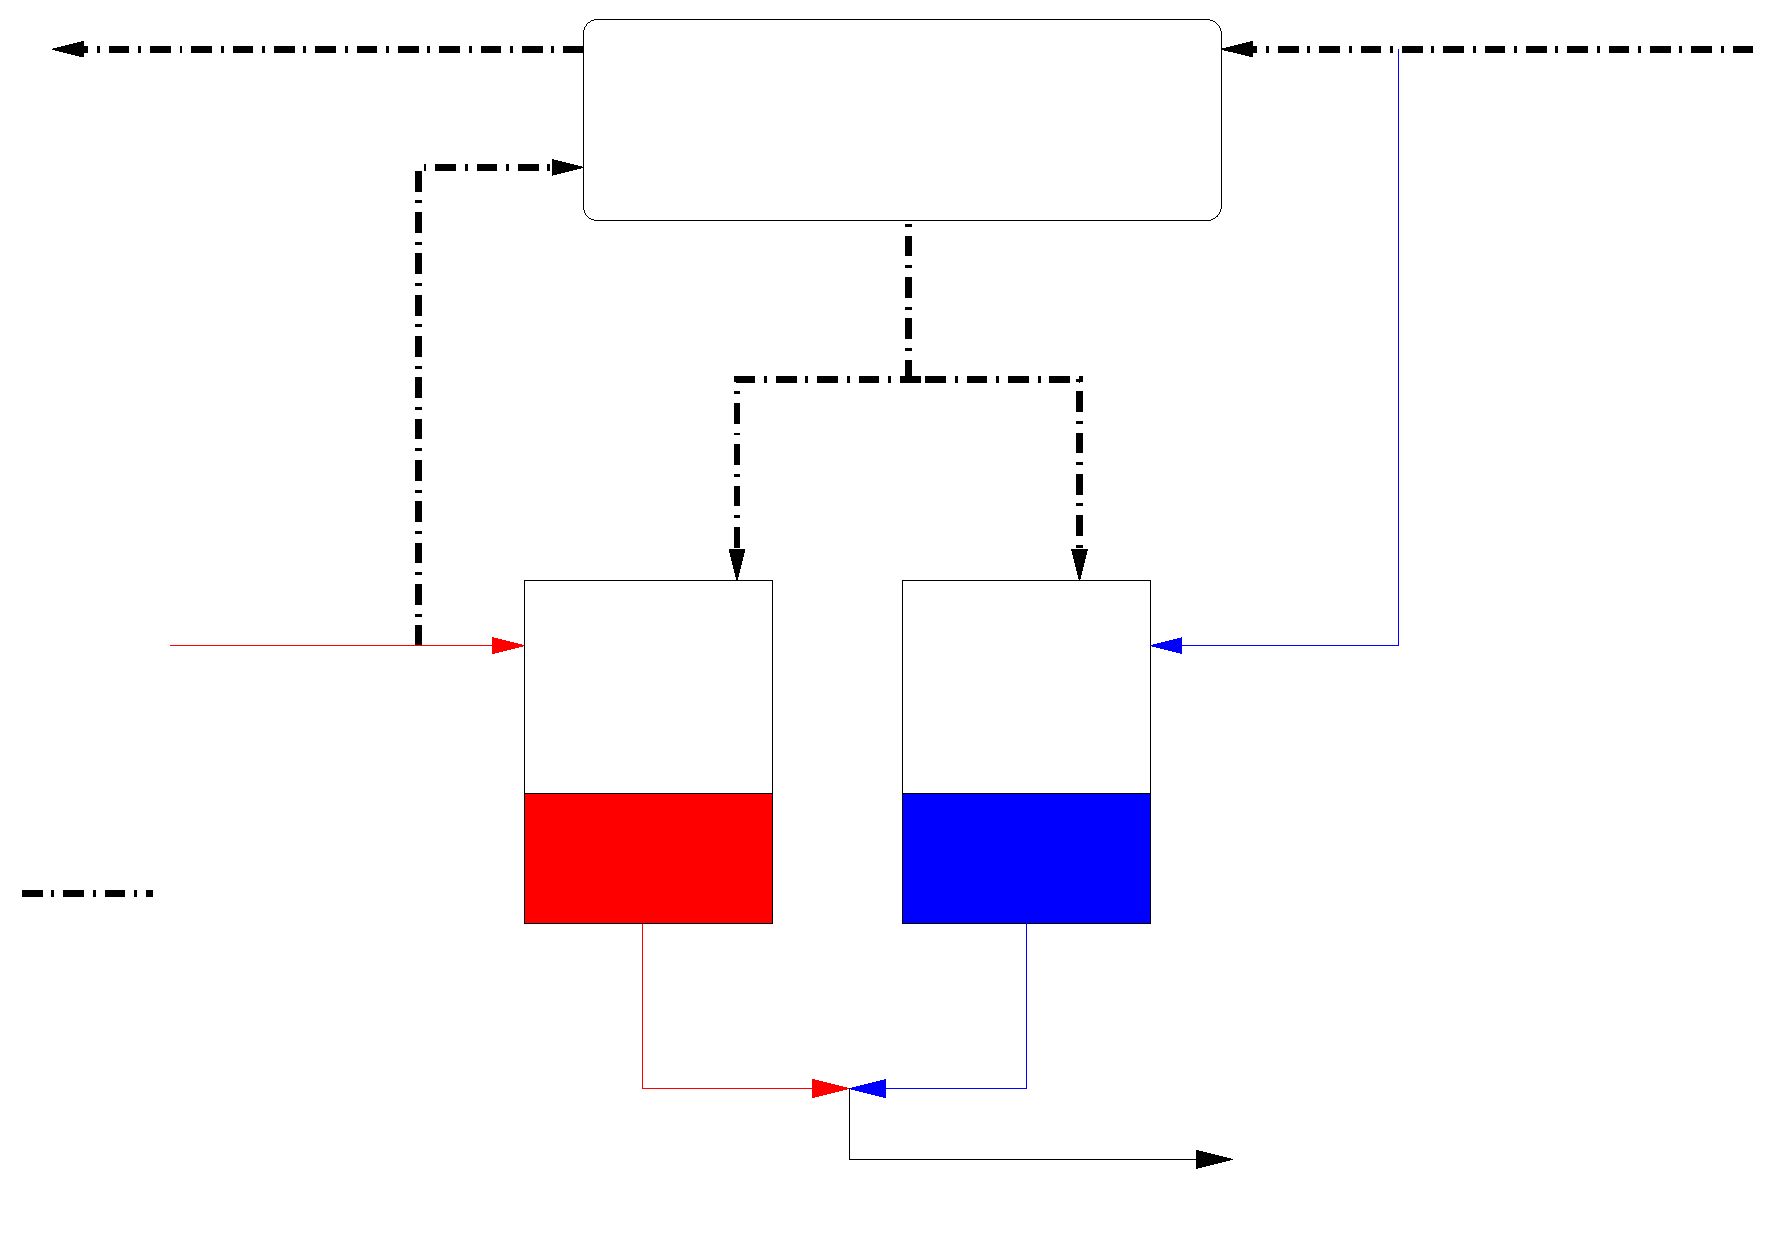
\includegraphics{sc/model}%
\end{picture}%
\setlength{\unitlength}{4144sp}%
%
\begingroup\makeatletter\ifx\SetFigFont\undefined%
\gdef\SetFigFont#1#2#3#4#5{%
  \reset@font\fontsize{#1}{#2pt}%
  \fontfamily{#3}\fontseries{#4}\fontshape{#5}%
  \selectfont}%
\fi\endgroup%
\begin{picture}(13273,9184)(182,-8648)
\put(1261,-4471){\makebox(0,0)[lb]{\smash{{\SetFigFont{17}{20.4}{\rmdefault}{\mddefault}{\updefault}{\color[rgb]{0,0,0}Shipments}%
}}}}
\put(7471,-5011){\makebox(0,0)[lb]{\smash{{\SetFigFont{20}{24.0}{\rmdefault}{\mddefault}{\updefault}{\color[rgb]{0,0,0}Orders}%
}}}}
\put(7471,-4696){\makebox(0,0)[lb]{\smash{{\SetFigFont{20}{24.0}{\rmdefault}{\mddefault}{\updefault}{\color[rgb]{0,0,0}Back-}%
}}}}
\put(5761,-241){\makebox(0,0)[lb]{\smash{{\SetFigFont{20}{24.0}{\rmdefault}{\mddefault}{\updefault}{\color[rgb]{0,0,0}Decision Maker}%
}}}}
\put(5581,-601){\makebox(0,0)[lb]{\smash{{\SetFigFont{14}{16.8}{\rmdefault}{\mddefault}{\updefault}{\color[rgb]{0,0,0}(policy implementer/ optimizer)}%
}}}}
\put(721,-361){\makebox(0,0)[lb]{\smash{{\SetFigFont{14}{16.8}{\rmdefault}{\mddefault}{\updefault}{\color[rgb]{0,0,0}(placed to }%
}}}}
\put(721,-661){\makebox(0,0)[lb]{\smash{{\SetFigFont{14}{16.8}{\rmdefault}{\mddefault}{\updefault}{\color[rgb]{0,0,0}upstream nodes)}%
}}}}
\put(1261,-4771){\makebox(0,0)[lb]{\smash{{\SetFigFont{14}{16.8}{\rmdefault}{\mddefault}{\updefault}{\color[rgb]{0,0,0}(from upstream nodes)}%
}}}}
\put(11116,-376){\makebox(0,0)[lb]{\smash{{\SetFigFont{14}{16.8}{\rmdefault}{\mddefault}{\updefault}{\color[rgb]{0,0,0}(placed by}%
}}}}
\put(11116,-646){\makebox(0,0)[lb]{\smash{{\SetFigFont{14}{16.8}{\rmdefault}{\mddefault}{\updefault}{\color[rgb]{0,0,0}downstream nodes)}%
}}}}
\put(9676,-7891){\makebox(0,0)[lb]{\smash{{\SetFigFont{14}{16.8}{\rmdefault}{\mddefault}{\updefault}{\color[rgb]{0,0,0}(to downstream nodes)}%
}}}}
\put(9676,-8566){\makebox(0,0)[lb]{\smash{{\SetFigFont{14}{16.8}{\rmdefault}{\mddefault}{\updefault}{\color[rgb]{0,0,0}(Demands satisfied)}%
}}}}
\put(1441,-6226){\makebox(0,0)[lb]{\smash{{\SetFigFont{14}{16.8}{\rmdefault}{\mddefault}{\updefault}{\color[rgb]{0,0,0}Information sharing}%
}}}}
\put(4321,-4876){\makebox(0,0)[lb]{\smash{{\SetFigFont{20}{24.0}{\rmdefault}{\mddefault}{\updefault}{\color[rgb]{0,0,0}Inventory}%
}}}}
\put(721,-61){\makebox(0,0)[lb]{\smash{{\SetFigFont{17}{20.4}{\rmdefault}{\mddefault}{\updefault}{\color[rgb]{0,0,0}Orders}%
}}}}
\put(11116,-61){\makebox(0,0)[lb]{\smash{{\SetFigFont{17}{20.4}{\rmdefault}{\mddefault}{\updefault}{\color[rgb]{0,0,0}Orders}%
}}}}
\put(9676,-8251){\makebox(0,0)[lb]{\smash{{\SetFigFont{17}{20.4}{\rmdefault}{\mddefault}{\updefault}{\color[rgb]{0,0,0}Shipments }%
}}}}
\end{picture}%
}}
\caption{Tank analogy for modeling a node.}
\label{fig:sc:nodemodel}
\end{figure}

The states in each node $i$ are:  the inventory in the node,
$\Inv_{pi} \forall p \in \mathcal{P}(i)$, and the backorders in the
node, $\BO_{pii'} \forall p \in \mathcal{P}(i), \forall i' \in \DN(i,p)$; two inputs:
the shipments made to each downstream node $j \in \DN(i,p)$, $S_{pij}$, and
the orders placed to each upstream node $j \in \UP(i,p)$, $O_{pij}$. The
shipments coming from the upstream nodes $S_{pji}, j \in \UP(i,p)$ and
the orders arriving from the downstream nodes $O_{pji}, j \in \DN(i,p)$
are the disturbances arriving to the node. Denoting discrete sample time by
integer $k$, the dynamic equations for node $i$ can be written as
\begin{align}
\Inv_{pi}(k+1) &= \Inv_{pi}(k) + \sum_{j \in \UP(i,p)}S_{pji}(k-\tau_{pji})
-\sum_{j \in \DN(i,p)}S_{pij}(k), \qquad \forall p \in \mathcal{P}(i)  \label{eq:sc:inventorybalance} \\
\BO_{pij}(k+1) &= \BO_{pij}(k) + O_{pji}(k) -S_{pij}(k),\qquad \forall
p \in \mathcal{P}(i), \forall j \in \DN(i,p)
\label{eq:sc:backorderbalance}
\end{align}
in which $\tau_{pji}$ is the transportation delay. We assume that there
are no delays for order transfers between the nodes.
Denoting $x_i(k) = \begin{bmatrix}\Inv_{pi}(k), p \in \mathcal{P}(i)  & \BO_{pij}(k),
   p \in \mathcal{P}(i),  j \in \DN(i,p)\end{bmatrix}'$,
$u_i(k) = \begin{bmatrix}S_{pij}, p \in \mathcal{P}(i), j \in \DN(i,p)&
  O_{pij'}, p \in \mathcal{P}(i),j' \in \UP(i,p)\end{bmatrix}'$, and
by using the lifting technique described in Chapter \ref{chap:scheduling},
the previous dynamic equations for the nodes
can be written in the familiar state space form for MPC applications 
\begin{equation}
x_i(k+1) = A_{ii}x_i(k) + B_{ii}u_i(k)+ \sum_{l\in\I \atop l \neq i}B_{il}u_l
%\label{eq:nodeequation}
\end{equation}
The decision maker shown in Figure \ref{fig:sc:nodemodel} can take
several different forms:
\begin{itemize}
\item Each decision maker can implement a simple ordering policy that
  depends only on the incoming shipments and orders. Such an ordering
  policy could be a PI controller to control the inventory levels, or
  $(\sigma,\Sigma)$ policies that are obtained from stochastic inventory
  control optimization. Such decision makers are implementations of
  classical control theory approaches to supply chain control.

\item {\textbf{Noncooperative MPC:}} Each decision maker can implement
  an MPC controller to regulate 
  its local states by optimizing a local objective function (for
  example, the profit function for the node). The nodes 
  can share information regarding upstream shipments,
  downstream orders, etc. This form of control is termed
  noncooperative MPC. 

\item {\textbf{Cooperative MPC:}} Each decision maker can implement an
  MPC controller  that 
  considers the effect of the nodes' decision on the entire supply chain
(for example, each node optimizes the supply chain profit
function). The nodes  still share information.

\item {\textbf{Centralized MPC:}} We can replace all the decision
  makers at the nodes with a 
  single decision maker at the supply chain level. This single
  decision maker  makes  decisions for all the nodes.
\end{itemize}  

The overall supply chain dynamic model is the individual node dynamic
equations  collected for all nodes $i \in \I$. The
only required change in the node dynamic equation
is for the retailer  and the production facility nodes.
\subsection*{Retailer models}
 For the retailer nodes $i \in \mathcal{R}$, the dynamic
equations are  modified as, 
\begin{align}
\Inv_{pi}(k+1) &= \Inv_i(k) + \sum_{j \in
  \UP(i,p)}S_{pji}(k-\tau_{pji}) - S_{pic}(k), \qquad \forall p \in \mathcal{P}(i)\\
\BO_{pi}(k+1) &= \BO_{pi}(k) + \Dem_{pic}(k)- S_{pic}(k),\qquad \forall p \in \mathcal{P}(i
\end{align}
in which $S_{pic}$ is the shipment made by the retailer, and
$\Dem_{pic}$ is the customer orders (demands).  \textit{The only disturbances in
the overall supply chain model are the customer demands} $d
= \begin{bmatrix} \Dem_{pic} \end{bmatrix}', p \in \mathcal{P}(i), i \in \mathcal{R}$, which
drive all the flows (shipments and orders) in the supply chain. 

\subsection*{Production facility models}

The production facility needs to be modeled separately because
material conversion takes place in this node. %The production facility model
%is the link between the raw material procurement dynamics and the finished
%product disbursement dynamics.
 In multiple product supply chains, the same production
facility handles multiple products. Thus a model for the production
facility needs to incorporate a scheduling model to optimize the
sequence of production. In this chapter, we assume that the production
facilities belong to  the first echelon. We further assume an ideal
supplier of raw materials to the production facilities, implying that
we have infinite supply of raw materials without transportation
delay. 

\paragraph{Planning models}
In this chapter, we shall use an ``approximate production model'' to 
model the production facility. In the approximate production model, we replace 
the detailed scheduling model with convex constraints that represent
the feasible region of production. This idea is similar to the process
attainable region \citep{sung:maravelias:2007}-a convex region of production
quantities for which there exists some feasible schedule. The process
attainable region can be computed by using computational geometry tools
\citep{sung:maravelias:2007, maravelias:sung:2009,
  sung:maravelias:2009} or parametric programming tools
\citep{li:ierapetritou:2010}. 
Let $\mathcal{M}$ be the set of production facility nodes. Then, for each $i \in \mathcal{M}$, the modified
dynamic equations for the final products are
\begin{align*}
\Inv_{pi}(k+1) &= \Inv_{pi}(k)+ S_{pim}(k) -\sum_{j \in
  \DN(i,p)}S_{pij}(k), \qquad \forall p \in \mathcal{P}(i)\\
\BO_{pij}(k+1) &= \BO_{pij}(k) + O_{pji}(k) -S_{pij}(k),\qquad \forall
p \in \mathcal{P}(i), \forall j \in \DN(i,p)
f(S_{ipm}(k)) &\leq 0
\end{align*}
in which $S_{pim}$ are the manipulated inputs denoting production of
product $p$  during the period. 
Note that, for multiproduct production facilities, each of the inputs
$S_{pim}$ for products $p \in \mathcal{P}$ are coupled by the
convex production feasibility constraint. The set $\mathcal{L}$
represents the set of products. 
\begin{equation*}
f(S_{1im}(k),S_{2ip}(k),\ldots,S_{pim}(k),\ldots) \leq 0
\end{equation*}


\paragraph{Scheduling models}
The state task network (STN) approach
is probably the most popular method to model a production facility in
which multiple products are produced using shared resources
\citep{kondili:pantelides:sargent:1993,shah:pantelides:sargent:1993}.
As described in Chapter \ref{chap:scheduling}, in STN modeling, the
final products, intermediates and raw materials are 
states that are processed using tasks like reactions, separation,
etc. These tasks can be carried out in units capable of
handling multiple tasks. A detailed schedule is the sequence of
operation of the tasks in the units so that a production objective
can be met at minimal cost without violating the scheduling
constraints.

Detailed scheduling models are formulated as mixed integer linear
programs (MILPs) or mixed integer nonlinear programs (MINLPs). If we
chose to model the production facility using a detailed scheduling
model, then the resulting supply chain MPC problems become mixed
integer programs. Although, research progress
has been made in the theory of MIQP and hybrid MPC (see
\citep{bemporad:morari:1999}), in this chapter, we do not consider
detailed scheduling models in the formulation of the supply
chain model. An example using a detailed scheduling model is provided
in Section \ref{sec:esc:multi}.


 

\subsection{Summary}
%\label{subsec:salient}
In this section, we wish to bring to the readers' attention, three
salient features of the supply chain dynamic model presented in this
section.

%\begin{enumerate}
%\item \textbf{Uncontrollable local models.} 
\paragraph{Uncontrollable local models} Controllability implies that there
  exist inputs that can move the state of the system from any initial
  state to any final state in finite time. Examining
  \eqref{eq:sc:inventorybalance} and \eqref{eq:sc:backorderbalance} for the 
  inventory and backorder balance  for node $i$, we observe that
  while nodes $j \in \UP(i,p)$ respond to orders $O_{pij}$ placed by node
  $i$, node $i$ has no knowledge of the subsequent dynamics of its own
  orders. Therefore, we need to provide the node 
  some model of how its orders affect the later shipments coming into the
  node. To do so in a noncooperative or decentralized control
  arrangement, we track another state (or output) $\IP_{pi}$ termed the
  inventory position. The dependence of orders on incoming
  shipments is modeled through the function $g(\cdot)$.
\begin{equation*}
\IP_{pi}(k+1) = \IP_{pi}(k) + \sum_{j \in \UP(i,p)}g(O_{pij}(k-\tau_{pji}))
- \sum_{j \in \DN(i)}S_{pij}(k) \qquad \forall p \in \mathcal{P}(i) 
\end{equation*}
In the centralized control framework, the actual dynamics of the entire
  supply chain is available to the decision maker, and the
  relationship of the orders at node $i$ to its subsequent incoming shipments is
  captured by the upstream nodes backorder balance equations and the
  supply chain performance metric. From Section
  \ref{sec:mpc:distributed:coop}, we know that cooperative MPC
  algorithms has complete model knowledge. Therefore, uncontrollable
  local models is not an issue when implementing cooperative MPC for
  supply chains.
\paragraph{Unstable models} The supply chain is
  modeled as a system of integrators whose
  response to an input step change is a ramp. Such systems
  need to be stabilized in the closed loop, otherwise the states can
  keep growing (think of it as backorders keep rising as time
  increases). Therefore, we emphasize establishing closed-loop
  properties 
  of the algorithms that we propose for supply chain optimization.
\paragraph{Stabilizable centralized model} We notice that all the
  nodes belonging to the manufacturing facilities are controllable
  because we manipulate the production rates. Therefore,  the
  manufacturing nodes do not require an inventory position
  model. Since the manufacturing 
  facility model has this property, the overall supply chain model is
  also controllable. The controllability of the centralized model is an
  important feature that we use to design closed-loop stable
  centralized and cooperative MPC frameworks for supply chain
  optimization.

\section{Example\footnote{The results this section, with the exception of
Sections \ref{sec:sc:supplycahin_example:robust},
\ref{sec:sc:supplychain_example:lssc} and the discussion on steady states, are slightly modified from Section 6 of
\citet{subramanian:rawlings:maravelias:2012} to reflect a coding error
that was corrected. }}
\label{sec:sc:supplychain_example}
We simulate the supply chain shown in Figure \ref{fig:sc:2stage} in this
section. The plant  has production delay of 2 time units and a
transportation delay of 2 time units and a single product. For
simplicity, we drop the index on product in this section. 

\paragraph{Production model}
As mentioned earlier, the production delay is 2 time units. However,
we assume that the manufacturer can start a batch of the product at
every sampling time. This assumption means that the manufacturer has
two units that can execute the task of producing the final product. 

\begin{figure}
\centering
\resizebox{0.75\textwidth}{!}{\begin{picture}(0,0)%
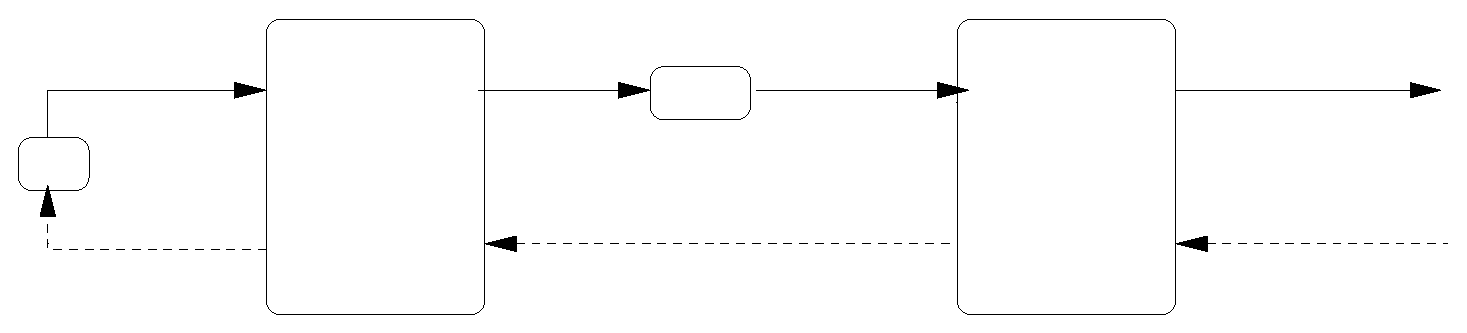
\includegraphics{2node}%
\end{picture}%
\setlength{\unitlength}{4144sp}%
%
\begingroup\makeatletter\ifx\SetFigFont\undefined%
\gdef\SetFigFont#1#2#3#4#5{%
  \reset@font\fontsize{#1}{#2pt}%
  \fontfamily{#3}\fontseries{#4}\fontshape{#5}%
  \selectfont}%
\fi\endgroup%
\begin{picture}(12701,2676)(166,-4459)
\put(9451,-2941){\makebox(0,0)[b]{\smash{{\SetFigFont{20}{24.0}{\familydefault}{\mddefault}{\updefault}{\color[rgb]{0,0,0}Retailer}%
}}}}
\put(181,-2266){\makebox(0,0)[lb]{\smash{{\SetFigFont{20}{24.0}{\familydefault}{\mddefault}{\updefault}{\color[rgb]{0,0,0}$S_{2p}(k-\tau_M)$}%
}}}}
\put(7066,-4291){\makebox(0,0)[lb]{\smash{{\SetFigFont{20}{24.0}{\familydefault}{\mddefault}{\updefault}{\color[rgb]{0,0,0}$O_{12}(k)$}%
}}}}
\put(811,-4291){\makebox(0,0)[lb]{\smash{{\SetFigFont{20}{24.0}{\familydefault}{\mddefault}{\updefault}{\color[rgb]{0,0,0}$S_{2p}(k)$}%
}}}}
\put(586,-3301){\makebox(0,0)[lb]{\smash{{\SetFigFont{20}{24.0}{\familydefault}{\mddefault}{\updefault}{\color[rgb]{0,0,0}$\tau_M = 2$}%
}}}}
\put(9451,-3571){\makebox(0,0)[b]{\smash{{\SetFigFont{20}{24.0}{\familydefault}{\mddefault}{\updefault}{\color[rgb]{0,0,0}Node $1$}%
}}}}
\put(3421,-3571){\makebox(0,0)[b]{\smash{{\SetFigFont{20}{24.0}{\familydefault}{\mddefault}{\updefault}{\color[rgb]{0,0,0}Node $2$}%
}}}}
\put(3421,-2941){\makebox(0,0)[b]{\smash{{\SetFigFont{20}{24.0}{\familydefault}{\mddefault}{\updefault}{\color[rgb]{0,0,0}Manufacturer}%
}}}}
\put(4591,-2311){\makebox(0,0)[lb]{\smash{{\SetFigFont{20}{24.0}{\familydefault}{\mddefault}{\updefault}{\color[rgb]{0,0,0}$S_{21}(k)$}%
}}}}
\put(5581,-2761){\makebox(0,0)[lb]{\smash{{\SetFigFont{20}{24.0}{\familydefault}{\mddefault}{\updefault}{\color[rgb]{0,0,0}$\tau_T=1$}%
}}}}
\put(10621,-2311){\makebox(0,0)[lb]{\smash{{\SetFigFont{20}{24.0}{\familydefault}{\mddefault}{\updefault}{\color[rgb]{0,0,0}$S_{1c}(k)$}%
}}}}
\put(11341,-4291){\makebox(0,0)[lb]{\smash{{\SetFigFont{20}{24.0}{\familydefault}{\mddefault}{\updefault}{\color[rgb]{0,0,0}$\Dem_{1c}(k)$}%
}}}}
\end{picture}%
}
\caption{Two-stage supply chain.}
\label{fig:sc:2stage}
\end{figure}
We label the retailer node $1$, with the states $\Inv_1$ and
$\BO_1$, the inventory and backorder at the retailer. The retailer
inputs $u_1$ consist of orders placed  and the shipments made by the retailer, $S_{1c}$ and
$O_{12}$.
We label the manufacturer  node $2$, with states $x_2$ consisting of
inventory $\Inv_2$ and backorder $\BO_2$. The manufacturer inputs
are the shipments made to the retailer $S_{21}$ and the production
e$S_{2m}$.  The demand $d(k) = \Dem_{1c}$. 

\paragraph{Models}
We write a  time invariant model  for the supply chain that is also the
 process model (because we assume that a batch may start at every
 time) by writing the inventory and backorder balance equation. These
 model for the retailer is:
\begin{equation}
\label{eq:sc:scheduling_example:R}
\underbrace{\begin{bmatrix}\Inv_1\\\BO_1\end{bmatrix}_{k+1}}_{x_1(k+1)} =
\underbrace{\begin{bmatrix}1&\\ &
    1\end{bmatrix}}_{A_1}\underbrace{\begin{bmatrix}\Inv_1\\\BO_1\end{bmatrix}_k}_{x_1(k)}
+\underbrace{\begin{bmatrix}-1 & 0 \\-1&
    0 \end{bmatrix}}_{B_{11}}\underbrace{\begin{bmatrix}S_{1c}\\O_{12}\end{bmatrix}_k}_{u_1(k)}
+\underbrace{\begin{bmatrix}-1 & 0 \\0&
    0 \end{bmatrix}}_{B_{22}^{(2)}}\underbrace{\begin{bmatrix}S_{21}\\S_{2m}\end{bmatrix}_{k-2}}_{u_2(k-2)}
+\underbrace{\begin{bmatrix} 0\\1\end{bmatrix}}_{B_d}\underbrace{\begin{bmatrix}\Dem_{1c}\end{bmatrix}_{k}}_{d(k)}
\end{equation}

The manufacturer state space is given by:
\begin{equation}
\label{eq:sc:scheduling_example:M}
\underbrace{\begin{bmatrix}\Inv_2\\\BO_2\end{bmatrix}_{k+1}}_{x_2(k+1)} =
\underbrace{\begin{bmatrix}1&\\ &
    1\end{bmatrix}}_{A_2}\underbrace{\begin{bmatrix}\Inv_2\\\BO_2\end{bmatrix}_k}_{x_2(k)}
+\underbrace{\begin{bmatrix}-1 & 0 \\-1&
    0 \end{bmatrix}}_{B_{22}}\underbrace{\begin{bmatrix}S_{21}\\S_{2m}\end{bmatrix}_k}_{u_2(k)}
+\underbrace{\begin{bmatrix}0 & 1 \\0&
    0 \end{bmatrix}}_{B_{22}^{(2)}}\underbrace{\begin{bmatrix}S_{21}\\S_{2m}\end{bmatrix}_{k-2}}_{u_2(k-2)}
+\underbrace{\begin{bmatrix} 0 & 0 \\0 &1\end{bmatrix}}_{B_{12}}\underbrace{\begin{bmatrix}S_{1c}\\O_{12}\end{bmatrix}_{k}}_{u_1(k)}
\end{equation}

Notice that the retailer, by just using $u_1$ cannot move the states
from any initial condition to any final condition. We can easily
verify this using the Hautus lemma. This matrix $\begin{bmatrix} I-A_1 & B_{11} \end{bmatrix}$ is
rank-deficient. 

\paragraph{Steady state} From equations
\eqref{eq:sc:scheduling_example:R} and
\eqref{eq:sc:scheduling_example:M}, we notice that if $B_{11}u_1(k) + B_{21}^{(2)}u_2(k-2)+B_dd(k) = 0$ and
$B_{22}u_2(k)+B_{22}^{(2)}u_2(k-2)+B_{12}u_1(k) = 0$, then any
inventory and backorder level can be a steady-state. From the tanks
analogy, as long as all the flows in and out of the tank are equal,
any level inside the tank is steady. Hence, we have a degree of
freedom in choosing the steady state for the inventories and backorders. The steady states
for the inputs is determined by the nominal (steady state) demand. Since, we wish to
meet all demands, the steady state for backorders is zero. On the
other hand, we wish to maintain a safety stock, and so we
choose inventory targets to regulate around. In the discussion that follows, we use
$x$ to denote deviation from the steady state, i.e., we redefine $x
\leftarrow x-x_s$ in which $x_s =
(\Inv_{1,t},0,\Inv_{2,t},0)$, with $\Inv_t$ referring
to the inventory target.


\paragraph{Stage cost}
Each node (subsystem) has a local stage cost, given by
\begin{equation*}
\ell_1(x_1,u_1)  = \norm{x_1}^2_{Q_1} + \norm{u_1}^2_{R_1},\quad
\ell_2(x_2,u_2) = \norm{x_2}^2_{Q_2} + \norm{u_2}^2_{R_2}
\end{equation*}
The overall stage cost is $\ell(x,u) =
\ell_1(x_1,u_1)+\ell_2(x_2,u_2)$. The costs used are $Q_1=Q_2=
\diag(1,10)$ and $R_1=R_2 = diag(1,1)$.

\paragraph{Terminal cost}
For centralized and cooperative MPC, following the theory outlined in
Section \ref{sec:mpc:distributed:relaxation}, we chose the $P>0,a>0$ such that there exists a
stabilizing control law $\kappa_f(x)$ in the terminal region given by:
\begin{equation*}
\mathbb{X}_f = \lbrace x \mid x'Px \leq a \rbrace
\end{equation*}
We also choose a $\bar{V}>0$ and fix $\beta = \max{(1,\bar{V}/a)}$. The
positive definite matrix $P$ is of the form $\left[ \begin{smallmatrix}P_{11}&
  P_{12} \\ P_{12}' & P_{22}\end{smallmatrix} \right]$. We choose the local
terminal cost functions and the centralized terminal cost function as 
\begin{equation*}
V_f^{1}(x_1) = \norm{x_1}_{P_{11}}^2 \qquad 
%\label{eq:terminal_R}
%\end{equation*}
%\begin{equation*}
V_f^{2}(x_2) = \norm{x_2}_{P_{22}}^2 \qquad
%\label{eq:terminal_M}
%\end{equation*}
%and the centralized cost function
%\begin{equation*}
V_f(x) = \norm{x}_P^2
%\label{eq:terminal_C}
\end{equation*}

We now define the MPC cost functions. The subsystem cost functions
are for $i \in \lbrace 1,2 \rbrace$
\begin{equation*}
V_N^{i,\beta}(x_i(0),\bu_i) =
\sum_{j=0}^{N-1}\ell_i(x_i(j),u_i(j)) \\ 
+ \beta V_f^{i}(x_i(N))
\end{equation*}
while the overall cost function is:
\begin{equation*}
V_N^\beta(x,\bu) = \sum_{j=0}^{N-1}\ell(x(j),u(j)) + \beta V_f(x(N))
\end{equation*}
Note that since we defined the terminal costs differently for the
subsystems, the overall cost function 
is not the sum of the subsystem cost functions. 
Associated with each input, we also have the input constraint set
$\mathbb{U}_1$ and $\mathbb{U}_2$, which contain the minimum and maximum
shipments and orders that can flow through the supply chain. The
maximum shipment allowed was capped at $40$ units, while any positive
order could be placed (arbitrarily large constraint).

\subsection*{MPC implementation}
\paragraph{Ordering policies}
As mentioned in Section \ref{sec:sc:modeling}, the local retailer model
does not have knowledge of how the orders placed by the retailer
affects the supply chain. Therefore, in the implementation of
noncooperative and decentralized MPC, we need to incorporate an
ordering policy for the retailer. Since the manufacturer reacts to the
orders placed by the retailer, the closed-loop performance of the
supply chain is intimately connected to the ordering policy.
We study two ordering policies in this example:
\begin{enumerate}
\item Order-up-to policy: The order-up-to  policy can be viewed as a
  saturated proportional  controller.
\begin{equation}
    O_{12}(k) = \begin{cases} \Inv_t-\Inv_1(k) & \text{if $\Inv_1 \leq \Inv_t$} \\
            0 & \text{otherwise}  \end{cases}
\end{equation}
in which $\Inv_t$ is the inventory target.
 
\item Inventory position control: In inventory position control, the
  retailer, instead of controlling the inventory, controls the
  inventory position, which is a controlled output defined as:
 \begin{equation}
   \IP(k) = \Inv_1(k)-S_{1c}(k) + O_{12}(k)
  \end{equation}
  Inventory position control introduces a new
  controlled output that is a function of the state and input. We
  penalize the deviations of $\IP$ from the inventory target
  $\Inv_t$ in the optimizations.
\end{enumerate}

\paragraph{Distributed MPC}
In decentralized and noncooperative MPC with order-up-to policy, we
modify the retailer subproblem, subsystem-1  in \eqref{eq:mpc:distributed:ncoop:PNi},
by adding a constraint that enforces the order-up-to
policy. Similarly, for decentralized and noncooperative MPC with
inventory position control, we modify the retailer objective function
in the  subsystem-1 problem in \eqref{eq:mpc:distributed:ncoop:PNi} by
modifying the stage cost to penalize inventory position $\IP$. We
present the optimization problem  \eqref{eq:mpc:distributed:ncoop:PNi}
again here for convenience (Note that (i) We do not have state constraints
in this example following Assumption \ref{ass:mpc:noX}, (ii) the
terminal penalty is magnified using the parameter $\beta$.)
\begin{xalignat*}{2}
\mathbb{P}_{N,nc}^i(x_i;\mathbf{v}_{-i}):& \min_{\bu_i}{\sum_{j=0}^{N-1}
\ell_i(x_i(j),u_i(j)) +\beta V_{f,i}(x_i(N))}& \nonumber\\
&\text{s.t.~} x_i(j+1) = Ax_i(j) + Bu_i(j) +  \sum_{l \in \set{1,2,\ldots,M} \atop l \neq i}
B_{li} v_l(j) & j = \set{0,1,\ldots,N-1} \nonumber\\
& u_i(j) \in \mathbb{U}_i & j = \set{0,1,\ldots,N-1} \nonumber \\
&x_i(0) = x_i \nonumber
\end{xalignat*}


Decentralized and noncooperative MPC are implemented using Algorithm
\ref{alg:mpc:distributed:ncoop}. In decentralized MPC, the subsystems do not share
information. That is $\mathbf{\nu}_{-i}$ is assumed by each subsystem
to makes its local predictions. Therefore, in the supply chain
context, we add another source of inaccuracy with decentralized
control (to add to using ordering policies).


The subproblems for cooperative MPC are obtained by fixing the other
subsystem inputs in the centralized optimization
problem \label{eq:mpc:distributed:relaxation:PNx} (reproduced here for convenience). Cooperative MPC
is implemented using Algorithm \ref{alg:mpc:distributed:coop}. In centralized MPC, we
solve the overall problem $\mathbb{P}^\beta_N(x)$ given in
\eqref{eq:mpc:distributed:relaxation:PNx}. The parameter $\beta$ was
chosen as $1000$. 

\begin{xalignat*}{2}
\mathbb{P}_N(x):& \min_{\bu}V^\beta_N(x,\bu) & \nonumber \\
&\text{s.t.~} x(j+1) = Ax(j) + Bu(j), &  j =
\set{1,2,\ldots,N-1} \nonumber \\
&u(j) \in \mathbb{U} &  j =
\set{0,1,2,\ldots,N-1} \nonumber \\
&x(0) = x & \nonumber\\
\end{xalignat*}

\subsection{Nominal demands}
\label{sec:sc:supplychain_example:nominal}
We present the results of the different MPC
implementations for a nominal demand of $d = 8$. In each of the
simulations, the retailer starts with inventory $\Inv_1 = 47$ and the
manufacturer starts with inventory $\Inv_2 = 32$. The control objective
is to keep the inventories in the nodes as close to the target
inventory ($\Inv_1 = 45$ and $\Inv_2 = 30$)as possible while maintaining minimum backorder. 

Figure \ref{fig:sc:orderupto} compares the results of centralized,
cooperative, noncooperative and decentralized MPC in which we used the
order-up-to ordering policy.  Figure \ref{fig:sc:IP_x} compares the
results of same controllers, but using the inventory control policy.
\begin{figure}
\centering
\scriptsize
\resizebox{\textwidth}{!}{% GNUPLOT: LaTeX picture with Postscript
\begingroup
  \makeatletter
  \providecommand\color[2][]{%
    \GenericError{(gnuplot) \space\space\space\@spaces}{%
      Package color not loaded in conjunction with
      terminal option `colourtext'%
    }{See the gnuplot documentation for explanation.%
    }{Either use 'blacktext' in gnuplot or load the package
      color.sty in LaTeX.}%
    \renewcommand\color[2][]{}%
  }%
  \providecommand\includegraphics[2][]{%
    \GenericError{(gnuplot) \space\space\space\@spaces}{%
      Package graphicx or graphics not loaded%
    }{See the gnuplot documentation for explanation.%
    }{The gnuplot epslatex terminal needs graphicx.sty or graphics.sty.}%
    \renewcommand\includegraphics[2][]{}%
  }%
  \providecommand\rotatebox[2]{#2}%
  \@ifundefined{ifGPcolor}{%
    \newif\ifGPcolor
    \GPcolortrue
  }{}%
  \@ifundefined{ifGPblacktext}{%
    \newif\ifGPblacktext
    \GPblacktexttrue
  }{}%
  % define a \g@addto@macro without @ in the name:
  \let\gplgaddtomacro\g@addto@macro
  % define empty templates for all commands taking text:
  \gdef\gplbacktext{}%
  \gdef\gplfronttext{}%
  \makeatother
  \ifGPblacktext
    % no textcolor at all
    \def\colorrgb#1{}%
    \def\colorgray#1{}%
  \else
    % gray or color?
    \ifGPcolor
      \def\colorrgb#1{\color[rgb]{#1}}%
      \def\colorgray#1{\color[gray]{#1}}%
      \expandafter\def\csname LTw\endcsname{\color{white}}%
      \expandafter\def\csname LTb\endcsname{\color{black}}%
      \expandafter\def\csname LTa\endcsname{\color{black}}%
      \expandafter\def\csname LT0\endcsname{\color[rgb]{1,0,0}}%
      \expandafter\def\csname LT1\endcsname{\color[rgb]{0,1,0}}%
      \expandafter\def\csname LT2\endcsname{\color[rgb]{0,0,1}}%
      \expandafter\def\csname LT3\endcsname{\color[rgb]{1,0,1}}%
      \expandafter\def\csname LT4\endcsname{\color[rgb]{0,1,1}}%
      \expandafter\def\csname LT5\endcsname{\color[rgb]{1,1,0}}%
      \expandafter\def\csname LT6\endcsname{\color[rgb]{0,0,0}}%
      \expandafter\def\csname LT7\endcsname{\color[rgb]{1,0.3,0}}%
      \expandafter\def\csname LT8\endcsname{\color[rgb]{0.5,0.5,0.5}}%
    \else
      % gray
      \def\colorrgb#1{\color{black}}%
      \def\colorgray#1{\color[gray]{#1}}%
      \expandafter\def\csname LTw\endcsname{\color{white}}%
      \expandafter\def\csname LTb\endcsname{\color{black}}%
      \expandafter\def\csname LTa\endcsname{\color{black}}%
      \expandafter\def\csname LT0\endcsname{\color{black}}%
      \expandafter\def\csname LT1\endcsname{\color{black}}%
      \expandafter\def\csname LT2\endcsname{\color{black}}%
      \expandafter\def\csname LT3\endcsname{\color{black}}%
      \expandafter\def\csname LT4\endcsname{\color{black}}%
      \expandafter\def\csname LT5\endcsname{\color{black}}%
      \expandafter\def\csname LT6\endcsname{\color{black}}%
      \expandafter\def\csname LT7\endcsname{\color{black}}%
      \expandafter\def\csname LT8\endcsname{\color{black}}%
    \fi
  \fi
  \setlength{\unitlength}{0.0500bp}%
  \begin{picture}(7200.00,3024.00)%
    \gplgaddtomacro\gplbacktext{%
      \csname LTb\endcsname%
      \put(814,440){\makebox(0,0)[r]{\strut{} 20}}%
      \put(814,1020){\makebox(0,0)[r]{\strut{} 30}}%
      \put(814,1600){\makebox(0,0)[r]{\strut{} 40}}%
      \put(814,2179){\makebox(0,0)[r]{\strut{} 50}}%
      \put(814,2759){\makebox(0,0)[r]{\strut{} 60}}%
      \put(946,220){\makebox(0,0){\strut{} 0}}%
      \put(1433,220){\makebox(0,0){\strut{} 10}}%
      \put(1921,220){\makebox(0,0){\strut{} 20}}%
      \put(2408,220){\makebox(0,0){\strut{} 30}}%
      \put(2896,220){\makebox(0,0){\strut{} 40}}%
      \put(3383,220){\makebox(0,0){\strut{} 50}}%
      \put(176,1599){\rotatebox{-270}{\makebox(0,0){\strut{}Inventory-Retailer}}}%
    }%
    \gplgaddtomacro\gplfronttext{%
      \csname LTb\endcsname%
      \put(2396,833){\makebox(0,0)[r]{\strut{}dec}}%
      \csname LTb\endcsname%
      \put(2396,613){\makebox(0,0)[r]{\strut{}ncoop}}%
    }%
    \gplgaddtomacro\gplbacktext{%
      \csname LTb\endcsname%
      \put(4109,220){\makebox(0,0){\strut{} 0}}%
      \put(4544,220){\makebox(0,0){\strut{} 10}}%
      \put(4978,220){\makebox(0,0){\strut{} 20}}%
      \put(5413,220){\makebox(0,0){\strut{} 30}}%
      \put(5847,220){\makebox(0,0){\strut{} 40}}%
      \put(6282,220){\makebox(0,0){\strut{} 50}}%
      \put(6414,440){\makebox(0,0)[l]{\strut{} 0}}%
      \put(6414,904){\makebox(0,0)[l]{\strut{} 10}}%
      \put(6414,1368){\makebox(0,0)[l]{\strut{} 20}}%
      \put(6414,1831){\makebox(0,0)[l]{\strut{} 30}}%
      \put(6414,2295){\makebox(0,0)[l]{\strut{} 40}}%
      \put(6414,2759){\makebox(0,0)[l]{\strut{} 50}}%
      \put(7051,1599){\rotatebox{-270}{\makebox(0,0){\strut{}Inventory-Manufacturer}}}%
    }%
    \gplgaddtomacro\gplfronttext{%
      \csname LTb\endcsname%
      \put(5295,833){\makebox(0,0)[r]{\strut{}coop}}%
      \csname LTb\endcsname%
      \put(5295,613){\makebox(0,0)[r]{\strut{}cent}}%
    }%
    \gplbacktext
    \put(0,0){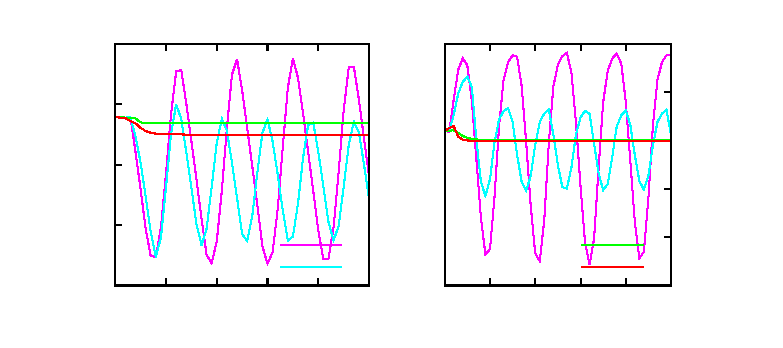
\includegraphics{sc/sS_demand}}%
    \gplfronttext
  \end{picture}%
\endgroup
}
\resizebox{\textwidth}{!}{% GNUPLOT: LaTeX picture with Postscript
\begingroup
  \makeatletter
  \providecommand\color[2][]{%
    \GenericError{(gnuplot) \space\space\space\@spaces}{%
      Package color not loaded in conjunction with
      terminal option `colourtext'%
    }{See the gnuplot documentation for explanation.%
    }{Either use 'blacktext' in gnuplot or load the package
      color.sty in LaTeX.}%
    \renewcommand\color[2][]{}%
  }%
  \providecommand\includegraphics[2][]{%
    \GenericError{(gnuplot) \space\space\space\@spaces}{%
      Package graphicx or graphics not loaded%
    }{See the gnuplot documentation for explanation.%
    }{The gnuplot epslatex terminal needs graphicx.sty or graphics.sty.}%
    \renewcommand\includegraphics[2][]{}%
  }%
  \providecommand\rotatebox[2]{#2}%
  \@ifundefined{ifGPcolor}{%
    \newif\ifGPcolor
    \GPcolortrue
  }{}%
  \@ifundefined{ifGPblacktext}{%
    \newif\ifGPblacktext
    \GPblacktexttrue
  }{}%
  % define a \g@addto@macro without @ in the name:
  \let\gplgaddtomacro\g@addto@macro
  % define empty templates for all commands taking text:
  \gdef\gplbacktext{}%
  \gdef\gplfronttext{}%
  \makeatother
  \ifGPblacktext
    % no textcolor at all
    \def\colorrgb#1{}%
    \def\colorgray#1{}%
  \else
    % gray or color?
    \ifGPcolor
      \def\colorrgb#1{\color[rgb]{#1}}%
      \def\colorgray#1{\color[gray]{#1}}%
      \expandafter\def\csname LTw\endcsname{\color{white}}%
      \expandafter\def\csname LTb\endcsname{\color{black}}%
      \expandafter\def\csname LTa\endcsname{\color{black}}%
      \expandafter\def\csname LT0\endcsname{\color[rgb]{1,0,0}}%
      \expandafter\def\csname LT1\endcsname{\color[rgb]{0,1,0}}%
      \expandafter\def\csname LT2\endcsname{\color[rgb]{0,0,1}}%
      \expandafter\def\csname LT3\endcsname{\color[rgb]{1,0,1}}%
      \expandafter\def\csname LT4\endcsname{\color[rgb]{0,1,1}}%
      \expandafter\def\csname LT5\endcsname{\color[rgb]{1,1,0}}%
      \expandafter\def\csname LT6\endcsname{\color[rgb]{0,0,0}}%
      \expandafter\def\csname LT7\endcsname{\color[rgb]{1,0.3,0}}%
      \expandafter\def\csname LT8\endcsname{\color[rgb]{0.5,0.5,0.5}}%
    \else
      % gray
      \def\colorrgb#1{\color{black}}%
      \def\colorgray#1{\color[gray]{#1}}%
      \expandafter\def\csname LTw\endcsname{\color{white}}%
      \expandafter\def\csname LTb\endcsname{\color{black}}%
      \expandafter\def\csname LTa\endcsname{\color{black}}%
      \expandafter\def\csname LT0\endcsname{\color{black}}%
      \expandafter\def\csname LT1\endcsname{\color{black}}%
      \expandafter\def\csname LT2\endcsname{\color{black}}%
      \expandafter\def\csname LT3\endcsname{\color{black}}%
      \expandafter\def\csname LT4\endcsname{\color{black}}%
      \expandafter\def\csname LT5\endcsname{\color{black}}%
      \expandafter\def\csname LT6\endcsname{\color{black}}%
      \expandafter\def\csname LT7\endcsname{\color{black}}%
      \expandafter\def\csname LT8\endcsname{\color{black}}%
    \fi
  \fi
  \setlength{\unitlength}{0.0500bp}%
  \begin{picture}(7200.00,3024.00)%
    \gplgaddtomacro\gplbacktext{%
      \csname LTb\endcsname%
      \put(814,704){\makebox(0,0)[r]{\strut{} 0}}%
      \put(814,1389){\makebox(0,0)[r]{\strut{} 10}}%
      \put(814,2074){\makebox(0,0)[r]{\strut{} 20}}%
      \put(814,2759){\makebox(0,0)[r]{\strut{} 30}}%
      \put(946,484){\makebox(0,0){\strut{} 0}}%
      \put(1433,484){\makebox(0,0){\strut{} 10}}%
      \put(1921,484){\makebox(0,0){\strut{} 20}}%
      \put(2408,484){\makebox(0,0){\strut{} 30}}%
      \put(2896,484){\makebox(0,0){\strut{} 40}}%
      \put(3383,484){\makebox(0,0){\strut{} 50}}%
      \put(176,1731){\rotatebox{-270}{\makebox(0,0){\strut{}Order-Retailer}}}%
      \put(2164,154){\makebox(0,0){\strut{}Time}}%
    }%
    \gplgaddtomacro\gplfronttext{%
    }%
    \gplgaddtomacro\gplbacktext{%
      \csname LTb\endcsname%
      \put(4109,484){\makebox(0,0){\strut{} 0}}%
      \put(4544,484){\makebox(0,0){\strut{} 10}}%
      \put(4978,484){\makebox(0,0){\strut{} 20}}%
      \put(5413,484){\makebox(0,0){\strut{} 30}}%
      \put(5847,484){\makebox(0,0){\strut{} 40}}%
      \put(6282,484){\makebox(0,0){\strut{} 50}}%
      \put(6414,704){\makebox(0,0)[l]{\strut{} 0}}%
      \put(6414,1732){\makebox(0,0)[l]{\strut{} 10}}%
      \put(6414,2759){\makebox(0,0)[l]{\strut{} 20}}%
      \put(7051,1731){\rotatebox{-270}{\makebox(0,0){\strut{}Production-Manufacturer}}}%
      \put(5195,154){\makebox(0,0){\strut{}Time}}%
    }%
    \gplgaddtomacro\gplfronttext{%
    }%
    \gplbacktext
    \put(0,0){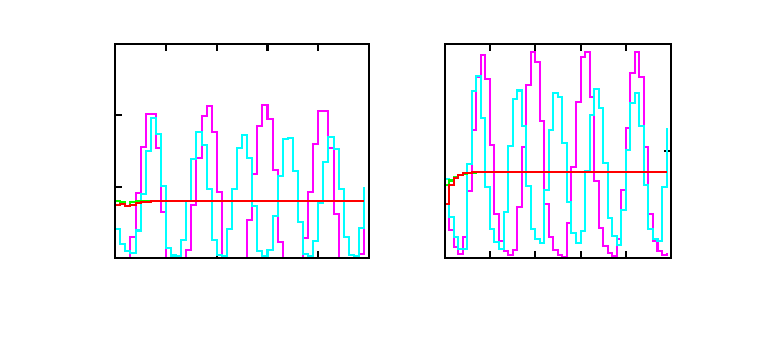
\includegraphics{sc/sS_demand_input}}%
    \gplfronttext
  \end{picture}%
\endgroup
}
\caption{Inventories and orders placed in the supply chain: Order-up-to policy (dec:
  decentralized, ncoop: noncooperative, coop: cooperative, cent: centralized).}
\label{fig:sc:orderupto}
\end{figure}

\begin{figure}
\centering
\scriptsize
\resizebox{\textwidth}{!}{% GNUPLOT: LaTeX picture with Postscript
\begingroup
  \makeatletter
  \providecommand\color[2][]{%
    \GenericError{(gnuplot) \space\space\space\@spaces}{%
      Package color not loaded in conjunction with
      terminal option `colourtext'%
    }{See the gnuplot documentation for explanation.%
    }{Either use 'blacktext' in gnuplot or load the package
      color.sty in LaTeX.}%
    \renewcommand\color[2][]{}%
  }%
  \providecommand\includegraphics[2][]{%
    \GenericError{(gnuplot) \space\space\space\@spaces}{%
      Package graphicx or graphics not loaded%
    }{See the gnuplot documentation for explanation.%
    }{The gnuplot epslatex terminal needs graphicx.sty or graphics.sty.}%
    \renewcommand\includegraphics[2][]{}%
  }%
  \providecommand\rotatebox[2]{#2}%
  \@ifundefined{ifGPcolor}{%
    \newif\ifGPcolor
    \GPcolortrue
  }{}%
  \@ifundefined{ifGPblacktext}{%
    \newif\ifGPblacktext
    \GPblacktexttrue
  }{}%
  % define a \g@addto@macro without @ in the name:
  \let\gplgaddtomacro\g@addto@macro
  % define empty templates for all commands taking text:
  \gdef\gplbacktext{}%
  \gdef\gplfronttext{}%
  \makeatother
  \ifGPblacktext
    % no textcolor at all
    \def\colorrgb#1{}%
    \def\colorgray#1{}%
  \else
    % gray or color?
    \ifGPcolor
      \def\colorrgb#1{\color[rgb]{#1}}%
      \def\colorgray#1{\color[gray]{#1}}%
      \expandafter\def\csname LTw\endcsname{\color{white}}%
      \expandafter\def\csname LTb\endcsname{\color{black}}%
      \expandafter\def\csname LTa\endcsname{\color{black}}%
      \expandafter\def\csname LT0\endcsname{\color[rgb]{1,0,0}}%
      \expandafter\def\csname LT1\endcsname{\color[rgb]{0,1,0}}%
      \expandafter\def\csname LT2\endcsname{\color[rgb]{0,0,1}}%
      \expandafter\def\csname LT3\endcsname{\color[rgb]{1,0,1}}%
      \expandafter\def\csname LT4\endcsname{\color[rgb]{0,1,1}}%
      \expandafter\def\csname LT5\endcsname{\color[rgb]{1,1,0}}%
      \expandafter\def\csname LT6\endcsname{\color[rgb]{0,0,0}}%
      \expandafter\def\csname LT7\endcsname{\color[rgb]{1,0.3,0}}%
      \expandafter\def\csname LT8\endcsname{\color[rgb]{0.5,0.5,0.5}}%
    \else
      % gray
      \def\colorrgb#1{\color{black}}%
      \def\colorgray#1{\color[gray]{#1}}%
      \expandafter\def\csname LTw\endcsname{\color{white}}%
      \expandafter\def\csname LTb\endcsname{\color{black}}%
      \expandafter\def\csname LTa\endcsname{\color{black}}%
      \expandafter\def\csname LT0\endcsname{\color{black}}%
      \expandafter\def\csname LT1\endcsname{\color{black}}%
      \expandafter\def\csname LT2\endcsname{\color{black}}%
      \expandafter\def\csname LT3\endcsname{\color{black}}%
      \expandafter\def\csname LT4\endcsname{\color{black}}%
      \expandafter\def\csname LT5\endcsname{\color{black}}%
      \expandafter\def\csname LT6\endcsname{\color{black}}%
      \expandafter\def\csname LT7\endcsname{\color{black}}%
      \expandafter\def\csname LT8\endcsname{\color{black}}%
    \fi
  \fi
  \setlength{\unitlength}{0.0500bp}%
  \begin{picture}(7200.00,3024.00)%
    \gplgaddtomacro\gplbacktext{%
      \csname LTb\endcsname%
      \put(814,440){\makebox(0,0)[r]{\strut{}-20}}%
      \put(814,1020){\makebox(0,0)[r]{\strut{} 0}}%
      \put(814,1600){\makebox(0,0)[r]{\strut{} 20}}%
      \put(814,2179){\makebox(0,0)[r]{\strut{} 40}}%
      \put(814,2759){\makebox(0,0)[r]{\strut{} 60}}%
      \put(946,220){\makebox(0,0){\strut{} 0}}%
      \put(1433,220){\makebox(0,0){\strut{} 10}}%
      \put(1921,220){\makebox(0,0){\strut{} 20}}%
      \put(2408,220){\makebox(0,0){\strut{} 30}}%
      \put(2896,220){\makebox(0,0){\strut{} 40}}%
      \put(3383,220){\makebox(0,0){\strut{} 50}}%
      \put(176,1599){\rotatebox{-270}{\makebox(0,0){\strut{}Inventory-Retailer}}}%
    }%
    \gplgaddtomacro\gplfronttext{%
      \csname LTb\endcsname%
      \put(2396,833){\makebox(0,0)[r]{\strut{}dec}}%
      \csname LTb\endcsname%
      \put(2396,613){\makebox(0,0)[r]{\strut{}ncoop}}%
    }%
    \gplgaddtomacro\gplbacktext{%
      \csname LTb\endcsname%
      \put(4109,220){\makebox(0,0){\strut{} 0}}%
      \put(4544,220){\makebox(0,0){\strut{} 10}}%
      \put(4978,220){\makebox(0,0){\strut{} 20}}%
      \put(5413,220){\makebox(0,0){\strut{} 30}}%
      \put(5847,220){\makebox(0,0){\strut{} 40}}%
      \put(6282,220){\makebox(0,0){\strut{} 50}}%
      \put(6414,440){\makebox(0,0)[l]{\strut{} 0}}%
      \put(6414,827){\makebox(0,0)[l]{\strut{} 10}}%
      \put(6414,1213){\makebox(0,0)[l]{\strut{} 20}}%
      \put(6414,1600){\makebox(0,0)[l]{\strut{} 30}}%
      \put(6414,1986){\makebox(0,0)[l]{\strut{} 40}}%
      \put(6414,2373){\makebox(0,0)[l]{\strut{} 50}}%
      \put(6414,2759){\makebox(0,0)[l]{\strut{} 60}}%
      \put(7051,1599){\rotatebox{-270}{\makebox(0,0){\strut{}Inventory-Manufacturer}}}%
    }%
    \gplgaddtomacro\gplfronttext{%
      \csname LTb\endcsname%
      \put(5295,833){\makebox(0,0)[r]{\strut{}coop}}%
      \csname LTb\endcsname%
      \put(5295,613){\makebox(0,0)[r]{\strut{}cent}}%
    }%
    \gplbacktext
    \put(0,0){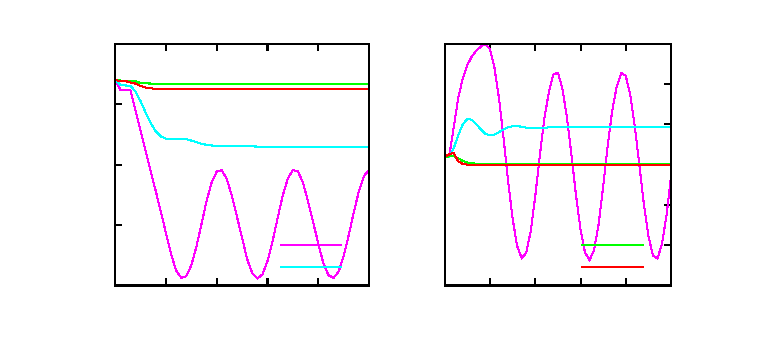
\includegraphics{sc/IP_dem}}%
    \gplfronttext
  \end{picture}%
\endgroup
}
\resizebox{\textwidth}{!}{% GNUPLOT: LaTeX picture with Postscript
\begingroup
  \makeatletter
  \providecommand\color[2][]{%
    \GenericError{(gnuplot) \space\space\space\@spaces}{%
      Package color not loaded in conjunction with
      terminal option `colourtext'%
    }{See the gnuplot documentation for explanation.%
    }{Either use 'blacktext' in gnuplot or load the package
      color.sty in LaTeX.}%
    \renewcommand\color[2][]{}%
  }%
  \providecommand\includegraphics[2][]{%
    \GenericError{(gnuplot) \space\space\space\@spaces}{%
      Package graphicx or graphics not loaded%
    }{See the gnuplot documentation for explanation.%
    }{The gnuplot epslatex terminal needs graphicx.sty or graphics.sty.}%
    \renewcommand\includegraphics[2][]{}%
  }%
  \providecommand\rotatebox[2]{#2}%
  \@ifundefined{ifGPcolor}{%
    \newif\ifGPcolor
    \GPcolortrue
  }{}%
  \@ifundefined{ifGPblacktext}{%
    \newif\ifGPblacktext
    \GPblacktexttrue
  }{}%
  % define a \g@addto@macro without @ in the name:
  \let\gplgaddtomacro\g@addto@macro
  % define empty templates for all commands taking text:
  \gdef\gplbacktext{}%
  \gdef\gplfronttext{}%
  \makeatother
  \ifGPblacktext
    % no textcolor at all
    \def\colorrgb#1{}%
    \def\colorgray#1{}%
  \else
    % gray or color?
    \ifGPcolor
      \def\colorrgb#1{\color[rgb]{#1}}%
      \def\colorgray#1{\color[gray]{#1}}%
      \expandafter\def\csname LTw\endcsname{\color{white}}%
      \expandafter\def\csname LTb\endcsname{\color{black}}%
      \expandafter\def\csname LTa\endcsname{\color{black}}%
      \expandafter\def\csname LT0\endcsname{\color[rgb]{1,0,0}}%
      \expandafter\def\csname LT1\endcsname{\color[rgb]{0,1,0}}%
      \expandafter\def\csname LT2\endcsname{\color[rgb]{0,0,1}}%
      \expandafter\def\csname LT3\endcsname{\color[rgb]{1,0,1}}%
      \expandafter\def\csname LT4\endcsname{\color[rgb]{0,1,1}}%
      \expandafter\def\csname LT5\endcsname{\color[rgb]{1,1,0}}%
      \expandafter\def\csname LT6\endcsname{\color[rgb]{0,0,0}}%
      \expandafter\def\csname LT7\endcsname{\color[rgb]{1,0.3,0}}%
      \expandafter\def\csname LT8\endcsname{\color[rgb]{0.5,0.5,0.5}}%
    \else
      % gray
      \def\colorrgb#1{\color{black}}%
      \def\colorgray#1{\color[gray]{#1}}%
      \expandafter\def\csname LTw\endcsname{\color{white}}%
      \expandafter\def\csname LTb\endcsname{\color{black}}%
      \expandafter\def\csname LTa\endcsname{\color{black}}%
      \expandafter\def\csname LT0\endcsname{\color{black}}%
      \expandafter\def\csname LT1\endcsname{\color{black}}%
      \expandafter\def\csname LT2\endcsname{\color{black}}%
      \expandafter\def\csname LT3\endcsname{\color{black}}%
      \expandafter\def\csname LT4\endcsname{\color{black}}%
      \expandafter\def\csname LT5\endcsname{\color{black}}%
      \expandafter\def\csname LT6\endcsname{\color{black}}%
      \expandafter\def\csname LT7\endcsname{\color{black}}%
      \expandafter\def\csname LT8\endcsname{\color{black}}%
    \fi
  \fi
  \setlength{\unitlength}{0.0500bp}%
  \begin{picture}(7200.00,3024.00)%
    \gplgaddtomacro\gplbacktext{%
      \csname LTb\endcsname%
      \put(814,704){\makebox(0,0)[r]{\strut{}-5}}%
      \put(814,1115){\makebox(0,0)[r]{\strut{} 0}}%
      \put(814,1526){\makebox(0,0)[r]{\strut{} 5}}%
      \put(814,1937){\makebox(0,0)[r]{\strut{} 10}}%
      \put(814,2348){\makebox(0,0)[r]{\strut{} 15}}%
      \put(814,2759){\makebox(0,0)[r]{\strut{} 20}}%
      \put(946,484){\makebox(0,0){\strut{} 0}}%
      \put(1433,484){\makebox(0,0){\strut{} 10}}%
      \put(1921,484){\makebox(0,0){\strut{} 20}}%
      \put(2408,484){\makebox(0,0){\strut{} 30}}%
      \put(2896,484){\makebox(0,0){\strut{} 40}}%
      \put(3383,484){\makebox(0,0){\strut{} 50}}%
      \put(176,1731){\rotatebox{-270}{\makebox(0,0){\strut{}Order-Retailer}}}%
      \put(2164,154){\makebox(0,0){\strut{}Time}}%
    }%
    \gplgaddtomacro\gplfronttext{%
    }%
    \gplgaddtomacro\gplbacktext{%
      \csname LTb\endcsname%
      \put(4109,484){\makebox(0,0){\strut{} 0}}%
      \put(4544,484){\makebox(0,0){\strut{} 10}}%
      \put(4978,484){\makebox(0,0){\strut{} 20}}%
      \put(5413,484){\makebox(0,0){\strut{} 30}}%
      \put(5847,484){\makebox(0,0){\strut{} 40}}%
      \put(6282,484){\makebox(0,0){\strut{} 50}}%
      \put(6414,704){\makebox(0,0)[l]{\strut{} 0}}%
      \put(6414,1389){\makebox(0,0)[l]{\strut{} 5}}%
      \put(6414,2074){\makebox(0,0)[l]{\strut{} 10}}%
      \put(6414,2759){\makebox(0,0)[l]{\strut{} 15}}%
      \put(7051,1731){\rotatebox{-270}{\makebox(0,0){\strut{}Production-Manufacturer}}}%
      \put(5195,154){\makebox(0,0){\strut{}Time}}%
    }%
    \gplgaddtomacro\gplfronttext{%
    }%
    \gplbacktext
    \put(0,0){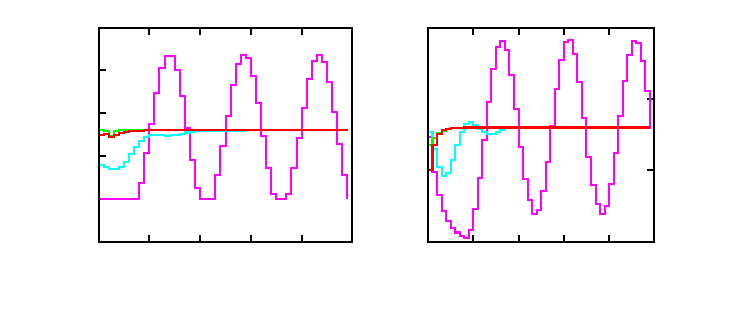
\includegraphics{sc/IP_dem_input}}%
    \gplfronttext
  \end{picture}%
\endgroup
}
\caption{Inventories and orders placed in the supply chain: Inventory position control (dec:
  decentralized, ncoop: noncooperative, coop: cooperative, cent: centralized).}
\label{fig:sc:IP_x}
\end{figure}

We defer discussion about the results to Section \ref{sec:sc:discussion}

\subsection{Stochastic demands}
\label{sec:sc:supplycahin_example:robust}
In \ref{sec:sc:supplychain_example:nominal}, we showed the response
using a model predictive controller for a supply chain observing
nominal demands. In this section, we show the results of implementing
the robust MPC algorithm presented in Section \ref{sec:mpc:robust}. We
consider the two node supply chain shown in Figure
\ref{fig:sc:2stage}, but with a nominal demand of $10$ units per time
period. The demand is assumed to be stochastic between $5$ and $15$
units per time period. In this example, we choose the retailer target
inventory $\Inv_{1,t} = 35$. 

Following the procedure outlined in Section \ref{sec:mpc:robust}, we
(i) design a stable cooperative MPC for the nominal system using the
methods outlined in the previous section, but with the tightened input
constraint sets to account for stochastic demands, and (ii) use the terminal
controller $\kappa_f(x) = Kx$ to account for the stochasticity in
demand. We used the technique outlined in \citet{rao:rawlings:1999} to find
$\kappa_f(x) = Kx$, such that all outstanding orders (backlogged
demands) from the previous time (if any) are satisfied at the current
sampling time. We chose the gain $K$ such that
$(A+BK)e$ implied that error in the backorder state was zero. Recall
that $e(k) = x(k)-z(k)$; the deviation between the actual state and
the nominal state. Hence, there is a delay
of 1 sampling time before the system reacts to the stochastic
demands. 


In Figure \ref{fig:sc:supplychain_example:CL1}, we show the closed-loop response 
nominal closed-loop response of the  inventory at the retailer for
cooperative MPC responding to a stochastic demand signal.  We also show the cost-function $V^\beta_N(z,\tilde{\mathbf{v}})$ and
$V^\beta_N(x,\tilde{\mathbf{v}})$ to show that although the warm-start was
infeasible for the actual state, it was still feasible for the nominal
state and hence we could obtain the closed-loop guarantees for robust
cooperative MPC. We used $\bar{V} = 20000$. Hence, whenever the cost
function for the actual state was greater than $20000$, it meant that
the warm-start was infeasible. That is, the terminal state was not
inside the set $\mathbb{X}_f$. However, by design of cooperative
algorithm, the warm start always remains feasible for the nominal MPC
problem.

In Figure \ref{fig:sc:supplychain_example:CL2}, we show the closed-loop response using a
modified version of Algorithm \ref{alg:mpc:robust} discussed in Section \ref{sec:mpc:robust}.

\begin{figure}
\centering
\scriptsize
\resizebox{\textwidth}{!}{% GNUPLOT: LaTeX picture with Postscript
\begingroup
  \makeatletter
  \providecommand\color[2][]{%
    \GenericError{(gnuplot) \space\space\space\@spaces}{%
      Package color not loaded in conjunction with
      terminal option `colourtext'%
    }{See the gnuplot documentation for explanation.%
    }{Either use 'blacktext' in gnuplot or load the package
      color.sty in LaTeX.}%
    \renewcommand\color[2][]{}%
  }%
  \providecommand\includegraphics[2][]{%
    \GenericError{(gnuplot) \space\space\space\@spaces}{%
      Package graphicx or graphics not loaded%
    }{See the gnuplot documentation for explanation.%
    }{The gnuplot epslatex terminal needs graphicx.sty or graphics.sty.}%
    \renewcommand\includegraphics[2][]{}%
  }%
  \providecommand\rotatebox[2]{#2}%
  \@ifundefined{ifGPcolor}{%
    \newif\ifGPcolor
    \GPcolortrue
  }{}%
  \@ifundefined{ifGPblacktext}{%
    \newif\ifGPblacktext
    \GPblacktexttrue
  }{}%
  % define a \g@addto@macro without @ in the name:
  \let\gplgaddtomacro\g@addto@macro
  % define empty templates for all commands taking text:
  \gdef\gplbacktext{}%
  \gdef\gplfronttext{}%
  \makeatother
  \ifGPblacktext
    % no textcolor at all
    \def\colorrgb#1{}%
    \def\colorgray#1{}%
  \else
    % gray or color?
    \ifGPcolor
      \def\colorrgb#1{\color[rgb]{#1}}%
      \def\colorgray#1{\color[gray]{#1}}%
      \expandafter\def\csname LTw\endcsname{\color{white}}%
      \expandafter\def\csname LTb\endcsname{\color{black}}%
      \expandafter\def\csname LTa\endcsname{\color{black}}%
      \expandafter\def\csname LT0\endcsname{\color[rgb]{1,0,0}}%
      \expandafter\def\csname LT1\endcsname{\color[rgb]{0,1,0}}%
      \expandafter\def\csname LT2\endcsname{\color[rgb]{0,0,1}}%
      \expandafter\def\csname LT3\endcsname{\color[rgb]{1,0,1}}%
      \expandafter\def\csname LT4\endcsname{\color[rgb]{0,1,1}}%
      \expandafter\def\csname LT5\endcsname{\color[rgb]{1,1,0}}%
      \expandafter\def\csname LT6\endcsname{\color[rgb]{0,0,0}}%
      \expandafter\def\csname LT7\endcsname{\color[rgb]{1,0.3,0}}%
      \expandafter\def\csname LT8\endcsname{\color[rgb]{0.5,0.5,0.5}}%
    \else
      % gray
      \def\colorrgb#1{\color{black}}%
      \def\colorgray#1{\color[gray]{#1}}%
      \expandafter\def\csname LTw\endcsname{\color{white}}%
      \expandafter\def\csname LTb\endcsname{\color{black}}%
      \expandafter\def\csname LTa\endcsname{\color{black}}%
      \expandafter\def\csname LT0\endcsname{\color{black}}%
      \expandafter\def\csname LT1\endcsname{\color{black}}%
      \expandafter\def\csname LT2\endcsname{\color{black}}%
      \expandafter\def\csname LT3\endcsname{\color{black}}%
      \expandafter\def\csname LT4\endcsname{\color{black}}%
      \expandafter\def\csname LT5\endcsname{\color{black}}%
      \expandafter\def\csname LT6\endcsname{\color{black}}%
      \expandafter\def\csname LT7\endcsname{\color{black}}%
      \expandafter\def\csname LT8\endcsname{\color{black}}%
    \fi
  \fi
  \setlength{\unitlength}{0.0500bp}%
  \begin{picture}(7200.00,3024.00)%
    \gplgaddtomacro\gplbacktext{%
      \csname LTb\endcsname%
      \put(814,704){\makebox(0,0)[r]{\strut{} 0}}%
      \put(814,1218){\makebox(0,0)[r]{\strut{} 10}}%
      \put(814,1732){\makebox(0,0)[r]{\strut{} 20}}%
      \put(814,2245){\makebox(0,0)[r]{\strut{} 30}}%
      \put(814,2759){\makebox(0,0)[r]{\strut{} 40}}%
      \put(946,484){\makebox(0,0){\strut{} 0}}%
      \put(1433,484){\makebox(0,0){\strut{} 10}}%
      \put(1921,484){\makebox(0,0){\strut{} 20}}%
      \put(2408,484){\makebox(0,0){\strut{} 30}}%
      \put(2896,484){\makebox(0,0){\strut{} 40}}%
      \put(3383,484){\makebox(0,0){\strut{} 50}}%
      \put(176,1731){\rotatebox{-270}{\makebox(0,0){\strut{}Level in Tank-2}}}%
      \put(2164,154){\makebox(0,0){\strut{}Time}}%
      \put(2165,1115){\makebox(0,0)[l]{\strut{}$S_K(\infty)$ bound}}%
    }%
    \gplgaddtomacro\gplfronttext{%
      \csname LTb\endcsname%
      \put(2396,2586){\makebox(0,0)[r]{\strut{}Actual}}%
      \csname LTb\endcsname%
      \put(2396,2366){\makebox(0,0)[r]{\strut{}Nominal}}%
    }%
    \gplgaddtomacro\gplbacktext{%
      \csname LTb\endcsname%
      \put(4109,484){\makebox(0,0){\strut{} 0}}%
      \put(4517,484){\makebox(0,0){\strut{} 2}}%
      \put(4925,484){\makebox(0,0){\strut{} 4}}%
      \put(5334,484){\makebox(0,0){\strut{} 6}}%
      \put(5742,484){\makebox(0,0){\strut{} 8}}%
      \put(6150,484){\makebox(0,0){\strut{} 10}}%
      \put(6282,704){\makebox(0,0)[l]{\strut{} 0}}%
      \put(6282,1115){\makebox(0,0)[l]{\strut{} 100}}%
      \put(6282,1526){\makebox(0,0)[l]{\strut{} 200}}%
      \put(6282,1937){\makebox(0,0)[l]{\strut{} 300}}%
      \put(6282,2348){\makebox(0,0)[l]{\strut{} 400}}%
      \put(6282,2759){\makebox(0,0)[l]{\strut{} 500}}%
      \put(7051,1731){\rotatebox{-270}{\makebox(0,0){\strut{}Cost}}}%
      \put(5129,154){\makebox(0,0){\strut{}time}}%
    }%
    \gplgaddtomacro\gplfronttext{%
      \csname LTb\endcsname%
      \put(5163,2586){\makebox(0,0)[r]{\strut{}$V_N^\beta(x,\tilde{\mathbf{v}})$}}%
      \csname LTb\endcsname%
      \put(5163,2366){\makebox(0,0)[r]{\strut{}$V_N^\beta(z,\tilde{\mathbf{v}})$}}%
      \csname LTb\endcsname%
      \put(5163,2146){\makebox(0,0)[r]{\strut{}$\bar{V}$}}%
    }%
    \gplbacktext
    \put(0,0){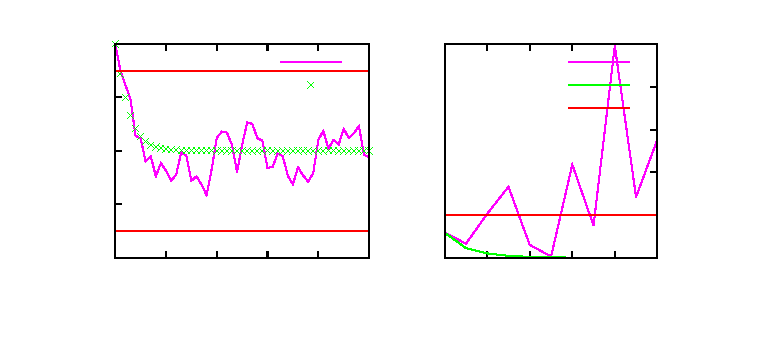
\includegraphics{mpc/CL1}}%
    \gplfronttext
  \end{picture}%
\endgroup
}
\caption{(Left) Closed-loop response (Right) Warm start rendered
  infeasible for actual state because of disturbance}
\label{fig:sc:supplychain_example:CL1}
\centering
\scriptsize
\resizebox{\textwidth}{!}{% GNUPLOT: LaTeX picture with Postscript
\begingroup
  \makeatletter
  \providecommand\color[2][]{%
    \GenericError{(gnuplot) \space\space\space\@spaces}{%
      Package color not loaded in conjunction with
      terminal option `colourtext'%
    }{See the gnuplot documentation for explanation.%
    }{Either use 'blacktext' in gnuplot or load the package
      color.sty in LaTeX.}%
    \renewcommand\color[2][]{}%
  }%
  \providecommand\includegraphics[2][]{%
    \GenericError{(gnuplot) \space\space\space\@spaces}{%
      Package graphicx or graphics not loaded%
    }{See the gnuplot documentation for explanation.%
    }{The gnuplot epslatex terminal needs graphicx.sty or graphics.sty.}%
    \renewcommand\includegraphics[2][]{}%
  }%
  \providecommand\rotatebox[2]{#2}%
  \@ifundefined{ifGPcolor}{%
    \newif\ifGPcolor
    \GPcolortrue
  }{}%
  \@ifundefined{ifGPblacktext}{%
    \newif\ifGPblacktext
    \GPblacktexttrue
  }{}%
  % define a \g@addto@macro without @ in the name:
  \let\gplgaddtomacro\g@addto@macro
  % define empty templates for all commands taking text:
  \gdef\gplbacktext{}%
  \gdef\gplfronttext{}%
  \makeatother
  \ifGPblacktext
    % no textcolor at all
    \def\colorrgb#1{}%
    \def\colorgray#1{}%
  \else
    % gray or color?
    \ifGPcolor
      \def\colorrgb#1{\color[rgb]{#1}}%
      \def\colorgray#1{\color[gray]{#1}}%
      \expandafter\def\csname LTw\endcsname{\color{white}}%
      \expandafter\def\csname LTb\endcsname{\color{black}}%
      \expandafter\def\csname LTa\endcsname{\color{black}}%
      \expandafter\def\csname LT0\endcsname{\color[rgb]{1,0,0}}%
      \expandafter\def\csname LT1\endcsname{\color[rgb]{0,1,0}}%
      \expandafter\def\csname LT2\endcsname{\color[rgb]{0,0,1}}%
      \expandafter\def\csname LT3\endcsname{\color[rgb]{1,0,1}}%
      \expandafter\def\csname LT4\endcsname{\color[rgb]{0,1,1}}%
      \expandafter\def\csname LT5\endcsname{\color[rgb]{1,1,0}}%
      \expandafter\def\csname LT6\endcsname{\color[rgb]{0,0,0}}%
      \expandafter\def\csname LT7\endcsname{\color[rgb]{1,0.3,0}}%
      \expandafter\def\csname LT8\endcsname{\color[rgb]{0.5,0.5,0.5}}%
    \else
      % gray
      \def\colorrgb#1{\color{black}}%
      \def\colorgray#1{\color[gray]{#1}}%
      \expandafter\def\csname LTw\endcsname{\color{white}}%
      \expandafter\def\csname LTb\endcsname{\color{black}}%
      \expandafter\def\csname LTa\endcsname{\color{black}}%
      \expandafter\def\csname LT0\endcsname{\color{black}}%
      \expandafter\def\csname LT1\endcsname{\color{black}}%
      \expandafter\def\csname LT2\endcsname{\color{black}}%
      \expandafter\def\csname LT3\endcsname{\color{black}}%
      \expandafter\def\csname LT4\endcsname{\color{black}}%
      \expandafter\def\csname LT5\endcsname{\color{black}}%
      \expandafter\def\csname LT6\endcsname{\color{black}}%
      \expandafter\def\csname LT7\endcsname{\color{black}}%
      \expandafter\def\csname LT8\endcsname{\color{black}}%
    \fi
  \fi
  \setlength{\unitlength}{0.0500bp}%
  \begin{picture}(7200.00,3024.00)%
    \gplgaddtomacro\gplbacktext{%
      \csname LTb\endcsname%
      \put(814,704){\makebox(0,0)[r]{\strut{} 10}}%
      \put(814,1389){\makebox(0,0)[r]{\strut{} 20}}%
      \put(814,2074){\makebox(0,0)[r]{\strut{} 30}}%
      \put(814,2759){\makebox(0,0)[r]{\strut{} 40}}%
      \put(946,484){\makebox(0,0){\strut{} 0}}%
      \put(2898,484){\makebox(0,0){\strut{} 10}}%
      \put(4851,484){\makebox(0,0){\strut{} 20}}%
      \put(6803,484){\makebox(0,0){\strut{} 30}}%
      \put(176,1731){\rotatebox{-270}{\makebox(0,0){\strut{}Inventory at Retailer}}}%
      \put(3874,154){\makebox(0,0){\strut{}Time}}%
      \put(4851,1732){\makebox(0,0)[l]{\strut{}Nominal state reset}}%
    }%
    \gplgaddtomacro\gplfronttext{%
      \csname LTb\endcsname%
      \put(4037,877){\makebox(0,0)[r]{\strut{}Actual}}%
      \csname LTb\endcsname%
      \put(5816,877){\makebox(0,0)[r]{\strut{}Nominal}}%
    }%
    \gplbacktext
    \put(0,0){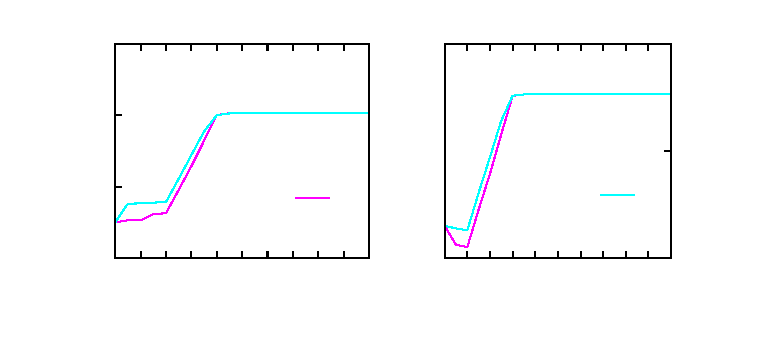
\includegraphics{CL2}}%
    \gplfronttext
  \end{picture}%
\endgroup
}
\caption{(Left) Closed-loop response. Notice that we reset the state
 t = 14, t = 24 when the cost is such that the warm start is
 feasible for the actual state (Right) Warm start rendered
 infeasible for actual state because of disturbance}
\label{fig:sc:supplychain_example:CL2}
\end{figure}


\subsection{Multi-echelon supply chain example}
\label{sec:sc:supplychain_example:lssc}
A critical step in the cooperative MPC algorithm (Algorithm -\ref{alg:mpc:distributed:coop})
using the Jacobi algorithm is the convex combination of the optimal
input with the values at the previous iterate that is taken in the
inner loop of the algorithm. The parameter $\omega_i$ limits the size
of the step taken in the descent direction. Since, it is required
that $\sum_{i=1}^{M} \omega_i=1$, the step sizes generated by the
Jacobi algorithm can become quite small as the number of subsystems
increase (and convergence is slow). As alluded in Section
\ref{sec:mpc:distributed:coop}, closely related to the Jacobi
algorithm is the Gauss-Seidel parallel optimization algorithm; in
which the subsystems move sequentially. The advantage in Gauss-Seidel
algorithm is that the subsystems can take full steps. The 
Gauss Seidel algorithm for subsystem $i$ can be written succinctly as:
\begin{align*}
 &\min_{\bu_i \in \mathbb{U}_i} V_N^\beta(x,\bu) \\
 &\text{s.t.~} \bu_l = \bu_l^{(p+1)}, \qquad l \in \set
 {1,2,\ldots,i-1}\\
 &\bu_l = \bu_l^{(p)}, \qquad l \in \set
 {i+1,i+2,\ldots,M}\\
\end{align*}
Upon obtaining the solution $\bu_i^0$ to the problem above, subsystem
$i$ sets its next iterate as $\bu_i^{(p+1)} = \bu_i^0$. As discussed in
  \citet[Section 3.3.5]{bertsekas:tsitsiklis:1989}, both these methods (Jacobi
and Gauss-Seidel) or any combination of these algorithms (blocks of
subsystem move sequentially; within every block, the subsystems move
in parallel) satisfy all the properties in Proposition
\ref{prop:mpc:distributed:jordan} (for convex problems) and Proposition
\ref{prop:mpc:distributed:jordan:converge} (with uncoupled
constraints). Hence, depending on the application, we could choose to
use Gauss-Seidel or a combination of Jacobi and Gauss-Seidel algorithm
in Cooperative MPC without losing any of the guarantees of Cooperative
MPC.

In this section, we present a combination Gauss-Seidel and Jacobi
algorithm (GSJ) that closely resembles the decision making hierarchy
in supply chains. Traditionally, in supply chains, the retailers
respond first to the customer demands. Upon receiving the orders from
the retailers, the distributors make their decisions. Therefore, the
current decision making paradigm in supply chains is a sequential
one. Hence, we propose to use a mixed Gauss-Seidel and Jacobi
optimization routine in cooperative MPC. The proposed optimization
proceeds as follows (for a three echelon supply chain): 
\begin{enumerate}
\item  The retailers, make their decisions in 
parallel, by fixing the upstream nodes decisions. Since only a subset
of the nodes are making their decisions in parallel, the convex
combination weight $\omega_i, i \in \mathcal{R}$ scale as
$\norm{\mathcal{R}}$ (the number of retailers),
\item  The distributors
obtain the retailer decisions and make their choices in parallel and,
\item  The manufacturers make their decisions after obtaining the
decisions of both the manufacturers and retailers.
\end{enumerate} 
The proposed algorithm has faster convergence when compared to the
Jacobi algorithm (see
Figure\ref{fig:sc:supplychain_example:lssc:convergence}).
Moreover, since the upstream nodes decisions
depend on the orders placed by the downstream node, in the Jacobi iterations, the upstream nodes have a disadvantage
because their optimizations are based on the previous iterate or
warm-start values of the downstream orders. On the other hand, in the
proposed method, the upstream nodes, optimize to react to the current
iterate of the downstream demands.

In Figure \ref{fig:sc:supplychain_example:lssc}, we show a 3 echelon
supply chain with 7 nodes. In this example, we consider only one
product. The transportation delay between nodes is 1 time unit,
while the production delay is 2 time units. As with the previous
example, we assume that the manufacturing unit can start a batch at
every sampling time. The stage cost for each node was chosen as
$\ell_i(x,u) = x'Qx +u'Ru$ with $Q = \text{diag}(1,10)$ and $R =
\text{diag}(1,1)$. The objective was to regulate to the inventory
targets (all backorder targets were zero). The nominal demand was $10$
units every period at each retailer node. In Table
\ref{tab:sc:supplychain_example:lssc}, we list the starting inventory
levels and the target inventory levels in each node. The maximum shipment from
one node to another was  $20$ units. The prediction horizon
was $N = 15$. We chose $\bar{V} = 5000$ and $a= 50$. We just implement
one iteration of the cooperative optimization algorithm, i.e.,
$\bar{p}=1$.
\begin{figure}[h]
\centering
\scriptsize
\resizebox{0.6\textwidth}{!}{\begin{picture}(0,0)%
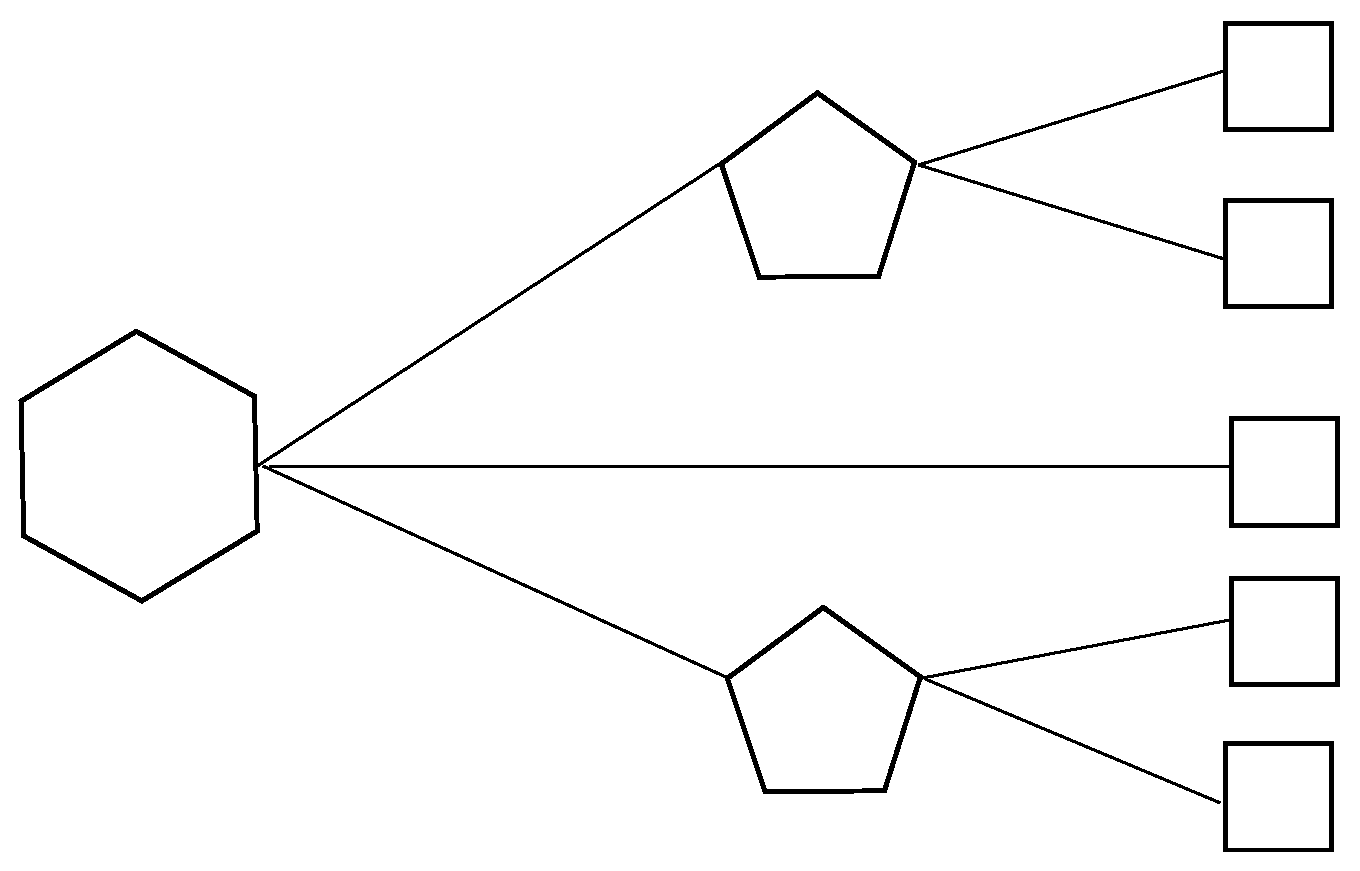
\includegraphics{esc/lssc}%
\end{picture}%
\setlength{\unitlength}{4144sp}%
%
\begingroup\makeatletter\ifx\SetFigFont\undefined%
\gdef\SetFigFont#1#2#3#4#5{%
  \reset@font\fontsize{#1}{#2pt}%
  \fontfamily{#3}\fontseries{#4}\fontshape{#5}%
  \selectfont}%
\fi\endgroup%
\begin{picture}(10101,6366)(1363,-5719)
\put(10801,164){\makebox(0,0)[lb]{\smash{{\SetFigFont{17}{20.4}{\familydefault}{\mddefault}{\updefault}{\color[rgb]{0,0,0}$R1$}%
}}}}
\put(2071,-2851){\makebox(0,0)[lb]{\smash{{\SetFigFont{17}{20.4}{\familydefault}{\mddefault}{\updefault}{\color[rgb]{0,0,0}$M1$}%
}}}}
\put(7246,-736){\makebox(0,0)[lb]{\smash{{\SetFigFont{17}{20.4}{\familydefault}{\mddefault}{\updefault}{\color[rgb]{0,0,0}$D1$}%
}}}}
\put(7291,-4741){\makebox(0,0)[lb]{\smash{{\SetFigFont{17}{20.4}{\familydefault}{\mddefault}{\updefault}{\color[rgb]{0,0,0}$D2$}%
}}}}
\put(10801,-5371){\makebox(0,0)[lb]{\smash{{\SetFigFont{17}{20.4}{\familydefault}{\mddefault}{\updefault}{\color[rgb]{0,0,0}$R4$}%
}}}}
\put(10846,-4111){\makebox(0,0)[lb]{\smash{{\SetFigFont{17}{20.4}{\familydefault}{\mddefault}{\updefault}{\color[rgb]{0,0,0}$R3$}%
}}}}
\put(10891,-2896){\makebox(0,0)[lb]{\smash{{\SetFigFont{17}{20.4}{\familydefault}{\mddefault}{\updefault}{\color[rgb]{0,0,0}$R5$}%
}}}}
\put(10801,-1231){\makebox(0,0)[lb]{\smash{{\SetFigFont{17}{20.4}{\familydefault}{\mddefault}{\updefault}{\color[rgb]{0,0,0}$R2$}%
}}}}
\end{picture}%
}
\caption{Multi-echelon supply chain studied}
\label{fig:sc:supplychain_example:lssc}
\end{figure}

\begin{table}[h]
\caption{Starting inventory and Inventory targets}
\begin{center}
\begin{tabular}{cccccccc}\toprule
& M1&D1&D2&R1&R2&R3&R4 \\
\midrule
Starting Inventory&40&37&38&28&39&29&36\\
Target Inventory&35&45&45&30&35&25&30\\
\bottomrule
\end{tabular}
\end{center}
\label{tab:sc:supplychain_example:lssc}
\end{table}


In Figure \ref{fig:sc:supplychain_example:lssc:convergence}, we show
the convergence of the three types of parallel optimization
algorithms. 

\begin{figure}
\centering
\scriptsize
\resizebox{\textwidth}{!}{% GNUPLOT: LaTeX picture with Postscript
\begingroup
  \makeatletter
  \providecommand\color[2][]{%
    \GenericError{(gnuplot) \space\space\space\@spaces}{%
      Package color not loaded in conjunction with
      terminal option `colourtext'%
    }{See the gnuplot documentation for explanation.%
    }{Either use 'blacktext' in gnuplot or load the package
      color.sty in LaTeX.}%
    \renewcommand\color[2][]{}%
  }%
  \providecommand\includegraphics[2][]{%
    \GenericError{(gnuplot) \space\space\space\@spaces}{%
      Package graphicx or graphics not loaded%
    }{See the gnuplot documentation for explanation.%
    }{The gnuplot epslatex terminal needs graphicx.sty or graphics.sty.}%
    \renewcommand\includegraphics[2][]{}%
  }%
  \providecommand\rotatebox[2]{#2}%
  \@ifundefined{ifGPcolor}{%
    \newif\ifGPcolor
    \GPcolortrue
  }{}%
  \@ifundefined{ifGPblacktext}{%
    \newif\ifGPblacktext
    \GPblacktexttrue
  }{}%
  % define a \g@addto@macro without @ in the name:
  \let\gplgaddtomacro\g@addto@macro
  % define empty templates for all commands taking text:
  \gdef\gplbacktext{}%
  \gdef\gplfronttext{}%
  \makeatother
  \ifGPblacktext
    % no textcolor at all
    \def\colorrgb#1{}%
    \def\colorgray#1{}%
  \else
    % gray or color?
    \ifGPcolor
      \def\colorrgb#1{\color[rgb]{#1}}%
      \def\colorgray#1{\color[gray]{#1}}%
      \expandafter\def\csname LTw\endcsname{\color{white}}%
      \expandafter\def\csname LTb\endcsname{\color{black}}%
      \expandafter\def\csname LTa\endcsname{\color{black}}%
      \expandafter\def\csname LT0\endcsname{\color[rgb]{1,0,0}}%
      \expandafter\def\csname LT1\endcsname{\color[rgb]{0,1,0}}%
      \expandafter\def\csname LT2\endcsname{\color[rgb]{0,0,1}}%
      \expandafter\def\csname LT3\endcsname{\color[rgb]{1,0,1}}%
      \expandafter\def\csname LT4\endcsname{\color[rgb]{0,1,1}}%
      \expandafter\def\csname LT5\endcsname{\color[rgb]{1,1,0}}%
      \expandafter\def\csname LT6\endcsname{\color[rgb]{0,0,0}}%
      \expandafter\def\csname LT7\endcsname{\color[rgb]{1,0.3,0}}%
      \expandafter\def\csname LT8\endcsname{\color[rgb]{0.5,0.5,0.5}}%
    \else
      % gray
      \def\colorrgb#1{\color{black}}%
      \def\colorgray#1{\color[gray]{#1}}%
      \expandafter\def\csname LTw\endcsname{\color{white}}%
      \expandafter\def\csname LTb\endcsname{\color{black}}%
      \expandafter\def\csname LTa\endcsname{\color{black}}%
      \expandafter\def\csname LT0\endcsname{\color{black}}%
      \expandafter\def\csname LT1\endcsname{\color{black}}%
      \expandafter\def\csname LT2\endcsname{\color{black}}%
      \expandafter\def\csname LT3\endcsname{\color{black}}%
      \expandafter\def\csname LT4\endcsname{\color{black}}%
      \expandafter\def\csname LT5\endcsname{\color{black}}%
      \expandafter\def\csname LT6\endcsname{\color{black}}%
      \expandafter\def\csname LT7\endcsname{\color{black}}%
      \expandafter\def\csname LT8\endcsname{\color{black}}%
    \fi
  \fi
  \setlength{\unitlength}{0.0500bp}%
  \begin{picture}(7200.00,3024.00)%
    \gplgaddtomacro\gplbacktext{%
      \csname LTb\endcsname%
      \put(946,704){\makebox(0,0)[r]{\strut{} 5}}%
      \put(946,910){\makebox(0,0)[r]{\strut{} 5.5}}%
      \put(946,1115){\makebox(0,0)[r]{\strut{} 6}}%
      \put(946,1321){\makebox(0,0)[r]{\strut{} 6.5}}%
      \put(946,1526){\makebox(0,0)[r]{\strut{} 7}}%
      \put(946,1732){\makebox(0,0)[r]{\strut{} 7.5}}%
      \put(946,1937){\makebox(0,0)[r]{\strut{} 8}}%
      \put(946,2143){\makebox(0,0)[r]{\strut{} 8.5}}%
      \put(946,2348){\makebox(0,0)[r]{\strut{} 9}}%
      \put(946,2554){\makebox(0,0)[r]{\strut{} 9.5}}%
      \put(946,2759){\makebox(0,0)[r]{\strut{} 10}}%
      \put(1598,484){\makebox(0,0){\strut{} 10}}%
      \put(2177,484){\makebox(0,0){\strut{} 20}}%
      \put(2755,484){\makebox(0,0){\strut{} 30}}%
      \put(3333,484){\makebox(0,0){\strut{} 40}}%
      \put(3912,484){\makebox(0,0){\strut{} 50}}%
      \put(4490,484){\makebox(0,0){\strut{} 60}}%
      \put(5068,484){\makebox(0,0){\strut{} 70}}%
      \put(5646,484){\makebox(0,0){\strut{} 80}}%
      \put(6225,484){\makebox(0,0){\strut{} 90}}%
      \put(6803,484){\makebox(0,0){\strut{} 100}}%
      \put(176,1731){\rotatebox{-270}{\makebox(0,0){\strut{}log $(V_N^\beta(\cdot))$}}}%
      \put(3940,154){\makebox(0,0){\strut{}Iteration}}%
    }%
    \gplgaddtomacro\gplfronttext{%
      \csname LTb\endcsname%
      \put(5816,2586){\makebox(0,0)[r]{\strut{}cent}}%
      \csname LTb\endcsname%
      \put(5816,2366){\makebox(0,0)[r]{\strut{}Jacobi}}%
      \csname LTb\endcsname%
      \put(5816,2146){\makebox(0,0)[r]{\strut{}Gauss-Siedel}}%
      \csname LTb\endcsname%
      \put(5816,1926){\makebox(0,0)[r]{\strut{}GSJ}}%
    }%
    \gplbacktext
    \put(0,0){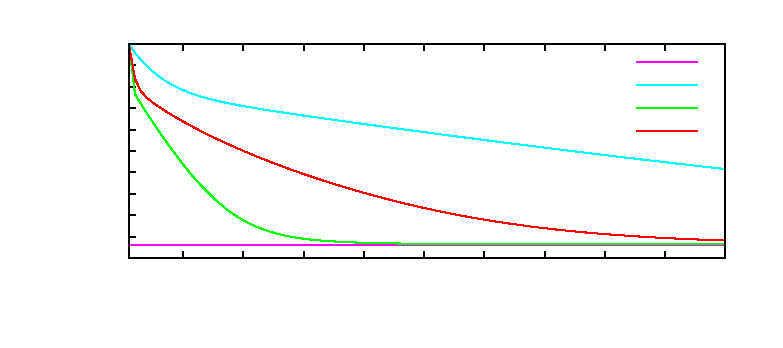
\includegraphics{sc/Conv}}%
    \gplfronttext
  \end{picture}%
\endgroup
}
\caption{Convergence of various parallel optimization algorithms for
  the supply chain example}
\label{fig:sc:supplychain_example:lssc:convergence}
\centering
\scriptsize
\resizebox{\textwidth}{!}{% GNUPLOT: LaTeX picture with Postscript
\begingroup
  \makeatletter
  \providecommand\color[2][]{%
    \GenericError{(gnuplot) \space\space\space\@spaces}{%
      Package color not loaded in conjunction with
      terminal option `colourtext'%
    }{See the gnuplot documentation for explanation.%
    }{Either use 'blacktext' in gnuplot or load the package
      color.sty in LaTeX.}%
    \renewcommand\color[2][]{}%
  }%
  \providecommand\includegraphics[2][]{%
    \GenericError{(gnuplot) \space\space\space\@spaces}{%
      Package graphicx or graphics not loaded%
    }{See the gnuplot documentation for explanation.%
    }{The gnuplot epslatex terminal needs graphicx.sty or graphics.sty.}%
    \renewcommand\includegraphics[2][]{}%
  }%
  \providecommand\rotatebox[2]{#2}%
  \@ifundefined{ifGPcolor}{%
    \newif\ifGPcolor
    \GPcolortrue
  }{}%
  \@ifundefined{ifGPblacktext}{%
    \newif\ifGPblacktext
    \GPblacktexttrue
  }{}%
  % define a \g@addto@macro without @ in the name:
  \let\gplgaddtomacro\g@addto@macro
  % define empty templates for all commands taking text:
  \gdef\gplbacktext{}%
  \gdef\gplfronttext{}%
  \makeatother
  \ifGPblacktext
    % no textcolor at all
    \def\colorrgb#1{}%
    \def\colorgray#1{}%
  \else
    % gray or color?
    \ifGPcolor
      \def\colorrgb#1{\color[rgb]{#1}}%
      \def\colorgray#1{\color[gray]{#1}}%
      \expandafter\def\csname LTw\endcsname{\color{white}}%
      \expandafter\def\csname LTb\endcsname{\color{black}}%
      \expandafter\def\csname LTa\endcsname{\color{black}}%
      \expandafter\def\csname LT0\endcsname{\color[rgb]{1,0,0}}%
      \expandafter\def\csname LT1\endcsname{\color[rgb]{0,1,0}}%
      \expandafter\def\csname LT2\endcsname{\color[rgb]{0,0,1}}%
      \expandafter\def\csname LT3\endcsname{\color[rgb]{1,0,1}}%
      \expandafter\def\csname LT4\endcsname{\color[rgb]{0,1,1}}%
      \expandafter\def\csname LT5\endcsname{\color[rgb]{1,1,0}}%
      \expandafter\def\csname LT6\endcsname{\color[rgb]{0,0,0}}%
      \expandafter\def\csname LT7\endcsname{\color[rgb]{1,0.3,0}}%
      \expandafter\def\csname LT8\endcsname{\color[rgb]{0.5,0.5,0.5}}%
    \else
      % gray
      \def\colorrgb#1{\color{black}}%
      \def\colorgray#1{\color[gray]{#1}}%
      \expandafter\def\csname LTw\endcsname{\color{white}}%
      \expandafter\def\csname LTb\endcsname{\color{black}}%
      \expandafter\def\csname LTa\endcsname{\color{black}}%
      \expandafter\def\csname LT0\endcsname{\color{black}}%
      \expandafter\def\csname LT1\endcsname{\color{black}}%
      \expandafter\def\csname LT2\endcsname{\color{black}}%
      \expandafter\def\csname LT3\endcsname{\color{black}}%
      \expandafter\def\csname LT4\endcsname{\color{black}}%
      \expandafter\def\csname LT5\endcsname{\color{black}}%
      \expandafter\def\csname LT6\endcsname{\color{black}}%
      \expandafter\def\csname LT7\endcsname{\color{black}}%
      \expandafter\def\csname LT8\endcsname{\color{black}}%
    \fi
  \fi
  \setlength{\unitlength}{0.0500bp}%
  \begin{picture}(7200.00,3024.00)%
    \gplgaddtomacro\gplbacktext{%
      \csname LTb\endcsname%
      \put(814,704){\makebox(0,0)[r]{\strut{}-4}}%
      \put(814,998){\makebox(0,0)[r]{\strut{}-2}}%
      \put(814,1291){\makebox(0,0)[r]{\strut{} 0}}%
      \put(814,1585){\makebox(0,0)[r]{\strut{} 2}}%
      \put(814,1878){\makebox(0,0)[r]{\strut{} 4}}%
      \put(814,2172){\makebox(0,0)[r]{\strut{} 6}}%
      \put(814,2465){\makebox(0,0)[r]{\strut{} 8}}%
      \put(814,2759){\makebox(0,0)[r]{\strut{} 10}}%
      \put(946,484){\makebox(0,0){\strut{} 0}}%
      \put(2117,484){\makebox(0,0){\strut{} 2}}%
      \put(3289,484){\makebox(0,0){\strut{} 4}}%
      \put(4460,484){\makebox(0,0){\strut{} 6}}%
      \put(5632,484){\makebox(0,0){\strut{} 8}}%
      \put(6803,484){\makebox(0,0){\strut{} 10}}%
      \put(176,1731){\rotatebox{-270}{\makebox(0,0){\strut{}log $(V_N^\beta(\cdot))$}}}%
      \put(3874,154){\makebox(0,0){\strut{}Time}}%
    }%
    \gplgaddtomacro\gplfronttext{%
      \csname LTb\endcsname%
      \put(5816,2586){\makebox(0,0)[r]{\strut{}cent}}%
      \csname LTb\endcsname%
      \put(5816,2366){\makebox(0,0)[r]{\strut{}GSJ}}%
      \csname LTb\endcsname%
      \put(5816,2146){\makebox(0,0)[r]{\strut{}Jacobi}}%
    }%
    \gplbacktext
    \put(0,0){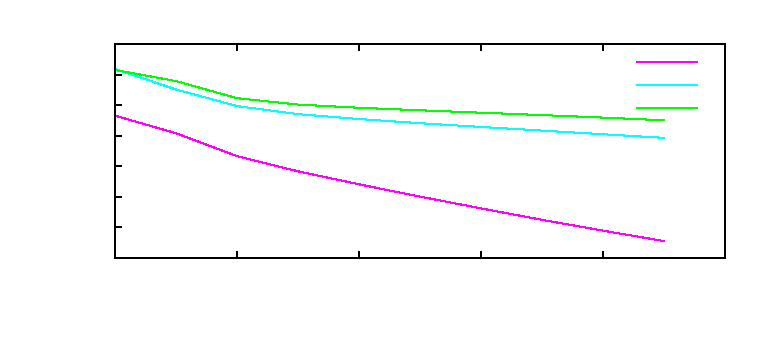
\includegraphics{sc/VN}}%
    \gplfronttext
  \end{picture}%
\endgroup
}
\caption{Open-loop prediction cost for cooperative MPC optimizations
  with 1 iteration}
\label{fig:sc:supplychain_example:lssc:VN}
\end{figure}

For this supply chain network, the Gauss-Seidel iterations converges
the fastest. In Figure
\ref{fig:sc:supplychain_example:lssc:Retailer}, we show the
inventory profile for  nodes $R1$ and $R2$  in the supply chain under centralized
control, the proposed Gauss-Seidel-Jacobi  algorithm
and the Jacobi algorithm. Not much difference in the
closed-loop performance can be observed. One reason for this
observation could be because the cooperative MPC
algorithm was initialized with the centralized optimal solution at
time $0$\footnote{There is no guarantee that will be such small differences in
if we initialize the cooperative MPC algorithm with the optimal
solution at $t=0$}. Hence, the warm start at time $t=1$ was close to the optimal
solution at time $1$.
\begin{figure}
\centering
\scriptsize
\resizebox{\textwidth}{!}{% GNUPLOT: LaTeX picture with Postscript
\begingroup
  \makeatletter
  \providecommand\color[2][]{%
    \GenericError{(gnuplot) \space\space\space\@spaces}{%
      Package color not loaded in conjunction with
      terminal option `colourtext'%
    }{See the gnuplot documentation for explanation.%
    }{Either use 'blacktext' in gnuplot or load the package
      color.sty in LaTeX.}%
    \renewcommand\color[2][]{}%
  }%
  \providecommand\includegraphics[2][]{%
    \GenericError{(gnuplot) \space\space\space\@spaces}{%
      Package graphicx or graphics not loaded%
    }{See the gnuplot documentation for explanation.%
    }{The gnuplot epslatex terminal needs graphicx.sty or graphics.sty.}%
    \renewcommand\includegraphics[2][]{}%
  }%
  \providecommand\rotatebox[2]{#2}%
  \@ifundefined{ifGPcolor}{%
    \newif\ifGPcolor
    \GPcolortrue
  }{}%
  \@ifundefined{ifGPblacktext}{%
    \newif\ifGPblacktext
    \GPblacktexttrue
  }{}%
  % define a \g@addto@macro without @ in the name:
  \let\gplgaddtomacro\g@addto@macro
  % define empty templates for all commands taking text:
  \gdef\gplbacktext{}%
  \gdef\gplfronttext{}%
  \makeatother
  \ifGPblacktext
    % no textcolor at all
    \def\colorrgb#1{}%
    \def\colorgray#1{}%
  \else
    % gray or color?
    \ifGPcolor
      \def\colorrgb#1{\color[rgb]{#1}}%
      \def\colorgray#1{\color[gray]{#1}}%
      \expandafter\def\csname LTw\endcsname{\color{white}}%
      \expandafter\def\csname LTb\endcsname{\color{black}}%
      \expandafter\def\csname LTa\endcsname{\color{black}}%
      \expandafter\def\csname LT0\endcsname{\color[rgb]{1,0,0}}%
      \expandafter\def\csname LT1\endcsname{\color[rgb]{0,1,0}}%
      \expandafter\def\csname LT2\endcsname{\color[rgb]{0,0,1}}%
      \expandafter\def\csname LT3\endcsname{\color[rgb]{1,0,1}}%
      \expandafter\def\csname LT4\endcsname{\color[rgb]{0,1,1}}%
      \expandafter\def\csname LT5\endcsname{\color[rgb]{1,1,0}}%
      \expandafter\def\csname LT6\endcsname{\color[rgb]{0,0,0}}%
      \expandafter\def\csname LT7\endcsname{\color[rgb]{1,0.3,0}}%
      \expandafter\def\csname LT8\endcsname{\color[rgb]{0.5,0.5,0.5}}%
    \else
      % gray
      \def\colorrgb#1{\color{black}}%
      \def\colorgray#1{\color[gray]{#1}}%
      \expandafter\def\csname LTw\endcsname{\color{white}}%
      \expandafter\def\csname LTb\endcsname{\color{black}}%
      \expandafter\def\csname LTa\endcsname{\color{black}}%
      \expandafter\def\csname LT0\endcsname{\color{black}}%
      \expandafter\def\csname LT1\endcsname{\color{black}}%
      \expandafter\def\csname LT2\endcsname{\color{black}}%
      \expandafter\def\csname LT3\endcsname{\color{black}}%
      \expandafter\def\csname LT4\endcsname{\color{black}}%
      \expandafter\def\csname LT5\endcsname{\color{black}}%
      \expandafter\def\csname LT6\endcsname{\color{black}}%
      \expandafter\def\csname LT7\endcsname{\color{black}}%
      \expandafter\def\csname LT8\endcsname{\color{black}}%
    \fi
  \fi
  \setlength{\unitlength}{0.0500bp}%
  \begin{picture}(7200.00,3024.00)%
    \gplgaddtomacro\gplbacktext{%
      \csname LTb\endcsname%
      \put(1078,704){\makebox(0,0)[r]{\strut{} 28}}%
      \put(1078,1115){\makebox(0,0)[r]{\strut{} 28.5}}%
      \put(1078,1526){\makebox(0,0)[r]{\strut{} 29}}%
      \put(1078,1937){\makebox(0,0)[r]{\strut{} 29.5}}%
      \put(1078,2348){\makebox(0,0)[r]{\strut{} 30}}%
      \put(1078,2759){\makebox(0,0)[r]{\strut{} 30.5}}%
      \put(1210,484){\makebox(0,0){\strut{} 0}}%
      \put(1427,484){\makebox(0,0){\strut{} 1}}%
      \put(1645,484){\makebox(0,0){\strut{} 2}}%
      \put(1862,484){\makebox(0,0){\strut{} 3}}%
      \put(2079,484){\makebox(0,0){\strut{} 4}}%
      \put(2297,484){\makebox(0,0){\strut{} 5}}%
      \put(2514,484){\makebox(0,0){\strut{} 6}}%
      \put(2731,484){\makebox(0,0){\strut{} 7}}%
      \put(2948,484){\makebox(0,0){\strut{} 8}}%
      \put(3166,484){\makebox(0,0){\strut{} 9}}%
      \put(3383,484){\makebox(0,0){\strut{} 10}}%
      \put(176,1731){\rotatebox{-270}{\makebox(0,0){\strut{}Inventory-R1}}}%
      \put(2296,154){\makebox(0,0){\strut{}Time}}%
    }%
    \gplgaddtomacro\gplfronttext{%
    }%
    \gplgaddtomacro\gplbacktext{%
      \csname LTb\endcsname%
      \put(4109,484){\makebox(0,0){\strut{} 0}}%
      \put(4300,484){\makebox(0,0){\strut{} 1}}%
      \put(4491,484){\makebox(0,0){\strut{} 2}}%
      \put(4682,484){\makebox(0,0){\strut{} 3}}%
      \put(4873,484){\makebox(0,0){\strut{} 4}}%
      \put(5064,484){\makebox(0,0){\strut{} 5}}%
      \put(5254,484){\makebox(0,0){\strut{} 6}}%
      \put(5445,484){\makebox(0,0){\strut{} 7}}%
      \put(5636,484){\makebox(0,0){\strut{} 8}}%
      \put(5827,484){\makebox(0,0){\strut{} 9}}%
      \put(6018,484){\makebox(0,0){\strut{} 10}}%
      \put(6150,704){\makebox(0,0)[l]{\strut{} 34.5}}%
      \put(6150,932){\makebox(0,0)[l]{\strut{} 35}}%
      \put(6150,1161){\makebox(0,0)[l]{\strut{} 35.5}}%
      \put(6150,1389){\makebox(0,0)[l]{\strut{} 36}}%
      \put(6150,1617){\makebox(0,0)[l]{\strut{} 36.5}}%
      \put(6150,1846){\makebox(0,0)[l]{\strut{} 37}}%
      \put(6150,2074){\makebox(0,0)[l]{\strut{} 37.5}}%
      \put(6150,2302){\makebox(0,0)[l]{\strut{} 38}}%
      \put(6150,2531){\makebox(0,0)[l]{\strut{} 38.5}}%
      \put(6150,2759){\makebox(0,0)[l]{\strut{} 39}}%
      \put(7051,1731){\rotatebox{-270}{\makebox(0,0){\strut{}Inventory-R2}}}%
      \put(5063,154){\makebox(0,0){\strut{}Time}}%
    }%
    \gplgaddtomacro\gplfronttext{%
      \csname LTb\endcsname%
      \put(5031,2586){\makebox(0,0)[r]{\strut{}cent}}%
      \csname LTb\endcsname%
      \put(5031,2366){\makebox(0,0)[r]{\strut{}GSJ}}%
      \csname LTb\endcsname%
      \put(5031,2146){\makebox(0,0)[r]{\strut{}Jacobi}}%
    }%
    \gplbacktext
    \put(0,0){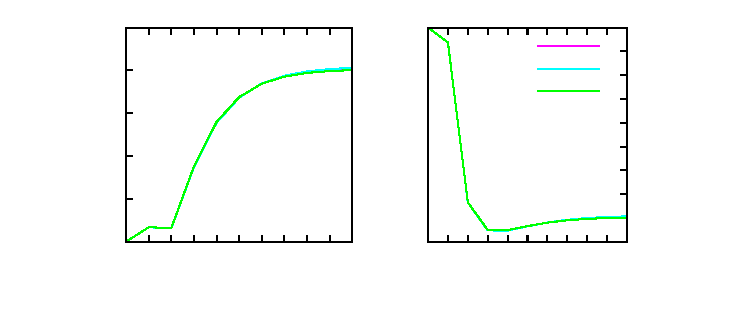
\includegraphics{sc/Rprofile}}%
    \gplfronttext
  \end{picture}%
\endgroup
}
\caption{Inventories in Retailer nodes 1 and 2 when cooperative MPC is
  initialized with centralized optimal input at $t=0$.}
\label{fig:sc:supplychain_example:lssc:Retailer}

\centering
\scriptsize
\resizebox{\textwidth}{!}{% GNUPLOT: LaTeX picture with Postscript
\begingroup
  \makeatletter
  \providecommand\color[2][]{%
    \GenericError{(gnuplot) \space\space\space\@spaces}{%
      Package color not loaded in conjunction with
      terminal option `colourtext'%
    }{See the gnuplot documentation for explanation.%
    }{Either use 'blacktext' in gnuplot or load the package
      color.sty in LaTeX.}%
    \renewcommand\color[2][]{}%
  }%
  \providecommand\includegraphics[2][]{%
    \GenericError{(gnuplot) \space\space\space\@spaces}{%
      Package graphicx or graphics not loaded%
    }{See the gnuplot documentation for explanation.%
    }{The gnuplot epslatex terminal needs graphicx.sty or graphics.sty.}%
    \renewcommand\includegraphics[2][]{}%
  }%
  \providecommand\rotatebox[2]{#2}%
  \@ifundefined{ifGPcolor}{%
    \newif\ifGPcolor
    \GPcolortrue
  }{}%
  \@ifundefined{ifGPblacktext}{%
    \newif\ifGPblacktext
    \GPblacktexttrue
  }{}%
  % define a \g@addto@macro without @ in the name:
  \let\gplgaddtomacro\g@addto@macro
  % define empty templates for all commands taking text:
  \gdef\gplbacktext{}%
  \gdef\gplfronttext{}%
  \makeatother
  \ifGPblacktext
    % no textcolor at all
    \def\colorrgb#1{}%
    \def\colorgray#1{}%
  \else
    % gray or color?
    \ifGPcolor
      \def\colorrgb#1{\color[rgb]{#1}}%
      \def\colorgray#1{\color[gray]{#1}}%
      \expandafter\def\csname LTw\endcsname{\color{white}}%
      \expandafter\def\csname LTb\endcsname{\color{black}}%
      \expandafter\def\csname LTa\endcsname{\color{black}}%
      \expandafter\def\csname LT0\endcsname{\color[rgb]{1,0,0}}%
      \expandafter\def\csname LT1\endcsname{\color[rgb]{0,1,0}}%
      \expandafter\def\csname LT2\endcsname{\color[rgb]{0,0,1}}%
      \expandafter\def\csname LT3\endcsname{\color[rgb]{1,0,1}}%
      \expandafter\def\csname LT4\endcsname{\color[rgb]{0,1,1}}%
      \expandafter\def\csname LT5\endcsname{\color[rgb]{1,1,0}}%
      \expandafter\def\csname LT6\endcsname{\color[rgb]{0,0,0}}%
      \expandafter\def\csname LT7\endcsname{\color[rgb]{1,0.3,0}}%
      \expandafter\def\csname LT8\endcsname{\color[rgb]{0.5,0.5,0.5}}%
    \else
      % gray
      \def\colorrgb#1{\color{black}}%
      \def\colorgray#1{\color[gray]{#1}}%
      \expandafter\def\csname LTw\endcsname{\color{white}}%
      \expandafter\def\csname LTb\endcsname{\color{black}}%
      \expandafter\def\csname LTa\endcsname{\color{black}}%
      \expandafter\def\csname LT0\endcsname{\color{black}}%
      \expandafter\def\csname LT1\endcsname{\color{black}}%
      \expandafter\def\csname LT2\endcsname{\color{black}}%
      \expandafter\def\csname LT3\endcsname{\color{black}}%
      \expandafter\def\csname LT4\endcsname{\color{black}}%
      \expandafter\def\csname LT5\endcsname{\color{black}}%
      \expandafter\def\csname LT6\endcsname{\color{black}}%
      \expandafter\def\csname LT7\endcsname{\color{black}}%
      \expandafter\def\csname LT8\endcsname{\color{black}}%
    \fi
  \fi
  \setlength{\unitlength}{0.0500bp}%
  \begin{picture}(7200.00,3024.00)%
    \gplgaddtomacro\gplbacktext{%
      \csname LTb\endcsname%
      \put(1078,704){\makebox(0,0)[r]{\strut{} 28}}%
      \put(1078,1115){\makebox(0,0)[r]{\strut{} 28.5}}%
      \put(1078,1526){\makebox(0,0)[r]{\strut{} 29}}%
      \put(1078,1937){\makebox(0,0)[r]{\strut{} 29.5}}%
      \put(1078,2348){\makebox(0,0)[r]{\strut{} 30}}%
      \put(1078,2759){\makebox(0,0)[r]{\strut{} 30.5}}%
      \put(1210,484){\makebox(0,0){\strut{} 0}}%
      \put(1427,484){\makebox(0,0){\strut{} 1}}%
      \put(1645,484){\makebox(0,0){\strut{} 2}}%
      \put(1862,484){\makebox(0,0){\strut{} 3}}%
      \put(2079,484){\makebox(0,0){\strut{} 4}}%
      \put(2297,484){\makebox(0,0){\strut{} 5}}%
      \put(2514,484){\makebox(0,0){\strut{} 6}}%
      \put(2731,484){\makebox(0,0){\strut{} 7}}%
      \put(2948,484){\makebox(0,0){\strut{} 8}}%
      \put(3166,484){\makebox(0,0){\strut{} 9}}%
      \put(3383,484){\makebox(0,0){\strut{} 10}}%
      \put(176,1731){\rotatebox{-270}{\makebox(0,0){\strut{}Inventory-R1}}}%
      \put(2296,154){\makebox(0,0){\strut{}Time}}%
    }%
    \gplgaddtomacro\gplfronttext{%
      \csname LTb\endcsname%
      \put(2396,1097){\makebox(0,0)[r]{\strut{}optimal}}%
      \csname LTb\endcsname%
      \put(2396,877){\makebox(0,0)[r]{\strut{}GSJ}}%
    }%
    \gplgaddtomacro\gplbacktext{%
      \csname LTb\endcsname%
      \put(4175,484){\makebox(0,0){\strut{} 0}}%
      \put(4359,484){\makebox(0,0){\strut{} 1}}%
      \put(4544,484){\makebox(0,0){\strut{} 2}}%
      \put(4728,484){\makebox(0,0){\strut{} 3}}%
      \put(4912,484){\makebox(0,0){\strut{} 4}}%
      \put(5097,484){\makebox(0,0){\strut{} 5}}%
      \put(5281,484){\makebox(0,0){\strut{} 6}}%
      \put(5465,484){\makebox(0,0){\strut{} 7}}%
      \put(5649,484){\makebox(0,0){\strut{} 8}}%
      \put(5834,484){\makebox(0,0){\strut{} 9}}%
      \put(6018,484){\makebox(0,0){\strut{} 10}}%
      \put(6150,704){\makebox(0,0)[l]{\strut{} 34.5}}%
      \put(6150,932){\makebox(0,0)[l]{\strut{} 35}}%
      \put(6150,1161){\makebox(0,0)[l]{\strut{} 35.5}}%
      \put(6150,1389){\makebox(0,0)[l]{\strut{} 36}}%
      \put(6150,1617){\makebox(0,0)[l]{\strut{} 36.5}}%
      \put(6150,1846){\makebox(0,0)[l]{\strut{} 37}}%
      \put(6150,2074){\makebox(0,0)[l]{\strut{} 37.5}}%
      \put(6150,2302){\makebox(0,0)[l]{\strut{} 38}}%
      \put(6150,2531){\makebox(0,0)[l]{\strut{} 38.5}}%
      \put(6150,2759){\makebox(0,0)[l]{\strut{} 39}}%
      \put(3955,1731){\rotatebox{-270}{\makebox(0,0){\strut{}Time}}}%
      \put(7051,1731){\rotatebox{-270}{\makebox(0,0){\strut{}Inventory-R2}}}%
      \put(5096,154){\makebox(0,0){\strut{}Time}}%
    }%
    \gplgaddtomacro\gplfronttext{%
    }%
    \gplbacktext
    \put(0,0){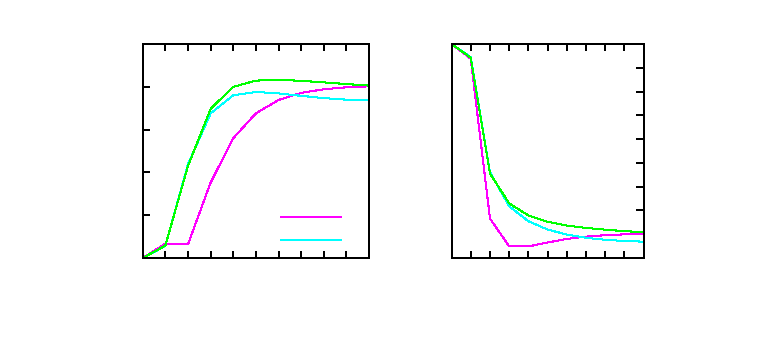
\includegraphics{sc/R1profile}}%
    \gplfronttext
  \end{picture}%
\endgroup
}
\caption{Inventories in Retailer nodes 1 and 2 when cooperative MPC is
initialized with suboptimal input at $t=0$}
\label{fig:sc:supplychain_example:lssc:bad}
\end{figure}

In Figure \ref{fig:sc:supplychain_example:lssc:bad}, we
show the closed-loop solutions when the supply chain was initialized
with a suboptimal solution at $t=0$.  In Figure \ref{fig:sc:supplychain_example:lssc:VN}, we
show the open-loop cost of the supply chain at each sampling time,
when the simulation was initialized with a suboptimal solution at $t=0$.


% \begin{figure}
% \centering
% \scriptsize
% \resizebox{\textwidth}{!}{% GNUPLOT: LaTeX picture with Postscript
\begingroup
  \makeatletter
  \providecommand\color[2][]{%
    \GenericError{(gnuplot) \space\space\space\@spaces}{%
      Package color not loaded in conjunction with
      terminal option `colourtext'%
    }{See the gnuplot documentation for explanation.%
    }{Either use 'blacktext' in gnuplot or load the package
      color.sty in LaTeX.}%
    \renewcommand\color[2][]{}%
  }%
  \providecommand\includegraphics[2][]{%
    \GenericError{(gnuplot) \space\space\space\@spaces}{%
      Package graphicx or graphics not loaded%
    }{See the gnuplot documentation for explanation.%
    }{The gnuplot epslatex terminal needs graphicx.sty or graphics.sty.}%
    \renewcommand\includegraphics[2][]{}%
  }%
  \providecommand\rotatebox[2]{#2}%
  \@ifundefined{ifGPcolor}{%
    \newif\ifGPcolor
    \GPcolortrue
  }{}%
  \@ifundefined{ifGPblacktext}{%
    \newif\ifGPblacktext
    \GPblacktexttrue
  }{}%
  % define a \g@addto@macro without @ in the name:
  \let\gplgaddtomacro\g@addto@macro
  % define empty templates for all commands taking text:
  \gdef\gplbacktext{}%
  \gdef\gplfronttext{}%
  \makeatother
  \ifGPblacktext
    % no textcolor at all
    \def\colorrgb#1{}%
    \def\colorgray#1{}%
  \else
    % gray or color?
    \ifGPcolor
      \def\colorrgb#1{\color[rgb]{#1}}%
      \def\colorgray#1{\color[gray]{#1}}%
      \expandafter\def\csname LTw\endcsname{\color{white}}%
      \expandafter\def\csname LTb\endcsname{\color{black}}%
      \expandafter\def\csname LTa\endcsname{\color{black}}%
      \expandafter\def\csname LT0\endcsname{\color[rgb]{1,0,0}}%
      \expandafter\def\csname LT1\endcsname{\color[rgb]{0,1,0}}%
      \expandafter\def\csname LT2\endcsname{\color[rgb]{0,0,1}}%
      \expandafter\def\csname LT3\endcsname{\color[rgb]{1,0,1}}%
      \expandafter\def\csname LT4\endcsname{\color[rgb]{0,1,1}}%
      \expandafter\def\csname LT5\endcsname{\color[rgb]{1,1,0}}%
      \expandafter\def\csname LT6\endcsname{\color[rgb]{0,0,0}}%
      \expandafter\def\csname LT7\endcsname{\color[rgb]{1,0.3,0}}%
      \expandafter\def\csname LT8\endcsname{\color[rgb]{0.5,0.5,0.5}}%
    \else
      % gray
      \def\colorrgb#1{\color{black}}%
      \def\colorgray#1{\color[gray]{#1}}%
      \expandafter\def\csname LTw\endcsname{\color{white}}%
      \expandafter\def\csname LTb\endcsname{\color{black}}%
      \expandafter\def\csname LTa\endcsname{\color{black}}%
      \expandafter\def\csname LT0\endcsname{\color{black}}%
      \expandafter\def\csname LT1\endcsname{\color{black}}%
      \expandafter\def\csname LT2\endcsname{\color{black}}%
      \expandafter\def\csname LT3\endcsname{\color{black}}%
      \expandafter\def\csname LT4\endcsname{\color{black}}%
      \expandafter\def\csname LT5\endcsname{\color{black}}%
      \expandafter\def\csname LT6\endcsname{\color{black}}%
      \expandafter\def\csname LT7\endcsname{\color{black}}%
      \expandafter\def\csname LT8\endcsname{\color{black}}%
    \fi
  \fi
  \setlength{\unitlength}{0.0500bp}%
  \begin{picture}(7200.00,3024.00)%
    \gplgaddtomacro\gplbacktext{%
      \csname LTb\endcsname%
      \put(814,704){\makebox(0,0)[r]{\strut{}-4}}%
      \put(814,998){\makebox(0,0)[r]{\strut{}-2}}%
      \put(814,1291){\makebox(0,0)[r]{\strut{} 0}}%
      \put(814,1585){\makebox(0,0)[r]{\strut{} 2}}%
      \put(814,1878){\makebox(0,0)[r]{\strut{} 4}}%
      \put(814,2172){\makebox(0,0)[r]{\strut{} 6}}%
      \put(814,2465){\makebox(0,0)[r]{\strut{} 8}}%
      \put(814,2759){\makebox(0,0)[r]{\strut{} 10}}%
      \put(946,484){\makebox(0,0){\strut{} 0}}%
      \put(2117,484){\makebox(0,0){\strut{} 2}}%
      \put(3289,484){\makebox(0,0){\strut{} 4}}%
      \put(4460,484){\makebox(0,0){\strut{} 6}}%
      \put(5632,484){\makebox(0,0){\strut{} 8}}%
      \put(6803,484){\makebox(0,0){\strut{} 10}}%
      \put(176,1731){\rotatebox{-270}{\makebox(0,0){\strut{}log $(V_N^\beta(\cdot))$}}}%
      \put(3874,154){\makebox(0,0){\strut{}Time}}%
    }%
    \gplgaddtomacro\gplfronttext{%
      \csname LTb\endcsname%
      \put(5816,2586){\makebox(0,0)[r]{\strut{}cent}}%
      \csname LTb\endcsname%
      \put(5816,2366){\makebox(0,0)[r]{\strut{}GSJ}}%
      \csname LTb\endcsname%
      \put(5816,2146){\makebox(0,0)[r]{\strut{}Jacobi}}%
    }%
    \gplbacktext
    \put(0,0){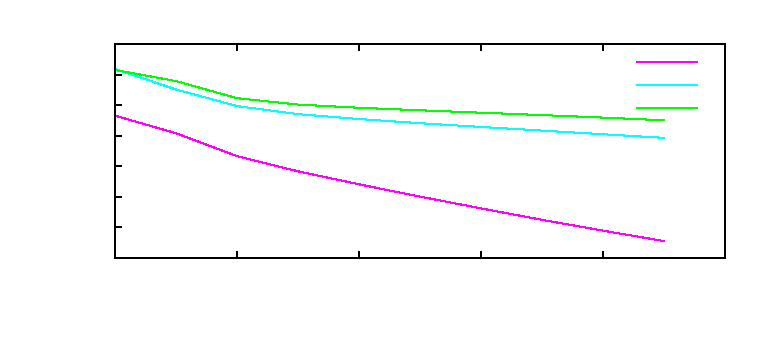
\includegraphics{sc/VN}}%
    \gplfronttext
  \end{picture}%
\endgroup
}
% %\resizebox{\textwidth}{!}{% GNUPLOT: LaTeX picture with Postscript
\begingroup
  \makeatletter
  \providecommand\color[2][]{%
    \GenericError{(gnuplot) \space\space\space\@spaces}{%
      Package color not loaded in conjunction with
      terminal option `colourtext'%
    }{See the gnuplot documentation for explanation.%
    }{Either use 'blacktext' in gnuplot or load the package
      color.sty in LaTeX.}%
    \renewcommand\color[2][]{}%
  }%
  \providecommand\includegraphics[2][]{%
    \GenericError{(gnuplot) \space\space\space\@spaces}{%
      Package graphicx or graphics not loaded%
    }{See the gnuplot documentation for explanation.%
    }{The gnuplot epslatex terminal needs graphicx.sty or graphics.sty.}%
    \renewcommand\includegraphics[2][]{}%
  }%
  \providecommand\rotatebox[2]{#2}%
  \@ifundefined{ifGPcolor}{%
    \newif\ifGPcolor
    \GPcolortrue
  }{}%
  \@ifundefined{ifGPblacktext}{%
    \newif\ifGPblacktext
    \GPblacktexttrue
  }{}%
  % define a \g@addto@macro without @ in the name:
  \let\gplgaddtomacro\g@addto@macro
  % define empty templates for all commands taking text:
  \gdef\gplbacktext{}%
  \gdef\gplfronttext{}%
  \makeatother
  \ifGPblacktext
    % no textcolor at all
    \def\colorrgb#1{}%
    \def\colorgray#1{}%
  \else
    % gray or color?
    \ifGPcolor
      \def\colorrgb#1{\color[rgb]{#1}}%
      \def\colorgray#1{\color[gray]{#1}}%
      \expandafter\def\csname LTw\endcsname{\color{white}}%
      \expandafter\def\csname LTb\endcsname{\color{black}}%
      \expandafter\def\csname LTa\endcsname{\color{black}}%
      \expandafter\def\csname LT0\endcsname{\color[rgb]{1,0,0}}%
      \expandafter\def\csname LT1\endcsname{\color[rgb]{0,1,0}}%
      \expandafter\def\csname LT2\endcsname{\color[rgb]{0,0,1}}%
      \expandafter\def\csname LT3\endcsname{\color[rgb]{1,0,1}}%
      \expandafter\def\csname LT4\endcsname{\color[rgb]{0,1,1}}%
      \expandafter\def\csname LT5\endcsname{\color[rgb]{1,1,0}}%
      \expandafter\def\csname LT6\endcsname{\color[rgb]{0,0,0}}%
      \expandafter\def\csname LT7\endcsname{\color[rgb]{1,0.3,0}}%
      \expandafter\def\csname LT8\endcsname{\color[rgb]{0.5,0.5,0.5}}%
    \else
      % gray
      \def\colorrgb#1{\color{black}}%
      \def\colorgray#1{\color[gray]{#1}}%
      \expandafter\def\csname LTw\endcsname{\color{white}}%
      \expandafter\def\csname LTb\endcsname{\color{black}}%
      \expandafter\def\csname LTa\endcsname{\color{black}}%
      \expandafter\def\csname LT0\endcsname{\color{black}}%
      \expandafter\def\csname LT1\endcsname{\color{black}}%
      \expandafter\def\csname LT2\endcsname{\color{black}}%
      \expandafter\def\csname LT3\endcsname{\color{black}}%
      \expandafter\def\csname LT4\endcsname{\color{black}}%
      \expandafter\def\csname LT5\endcsname{\color{black}}%
      \expandafter\def\csname LT6\endcsname{\color{black}}%
      \expandafter\def\csname LT7\endcsname{\color{black}}%
      \expandafter\def\csname LT8\endcsname{\color{black}}%
    \fi
  \fi
  \setlength{\unitlength}{0.0500bp}%
  \begin{picture}(7200.00,3024.00)%
    \gplgaddtomacro\gplbacktext{%
      \csname LTb\endcsname%
      \put(814,704){\makebox(0,0)[r]{\strut{} 0}}%
      \put(814,1389){\makebox(0,0)[r]{\strut{} 10}}%
      \put(814,2074){\makebox(0,0)[r]{\strut{} 20}}%
      \put(814,2759){\makebox(0,0)[r]{\strut{} 30}}%
      \put(946,484){\makebox(0,0){\strut{} 0}}%
      \put(1433,484){\makebox(0,0){\strut{} 10}}%
      \put(1921,484){\makebox(0,0){\strut{} 20}}%
      \put(2408,484){\makebox(0,0){\strut{} 30}}%
      \put(2896,484){\makebox(0,0){\strut{} 40}}%
      \put(3383,484){\makebox(0,0){\strut{} 50}}%
      \put(176,1731){\rotatebox{-270}{\makebox(0,0){\strut{}Order-Retailer}}}%
      \put(2164,154){\makebox(0,0){\strut{}Time}}%
    }%
    \gplgaddtomacro\gplfronttext{%
    }%
    \gplgaddtomacro\gplbacktext{%
      \csname LTb\endcsname%
      \put(4109,484){\makebox(0,0){\strut{} 0}}%
      \put(4544,484){\makebox(0,0){\strut{} 10}}%
      \put(4978,484){\makebox(0,0){\strut{} 20}}%
      \put(5413,484){\makebox(0,0){\strut{} 30}}%
      \put(5847,484){\makebox(0,0){\strut{} 40}}%
      \put(6282,484){\makebox(0,0){\strut{} 50}}%
      \put(6414,704){\makebox(0,0)[l]{\strut{} 0}}%
      \put(6414,1732){\makebox(0,0)[l]{\strut{} 10}}%
      \put(6414,2759){\makebox(0,0)[l]{\strut{} 20}}%
      \put(7051,1731){\rotatebox{-270}{\makebox(0,0){\strut{}Production-Manufacturer}}}%
      \put(5195,154){\makebox(0,0){\strut{}Time}}%
    }%
    \gplgaddtomacro\gplfronttext{%
    }%
    \gplbacktext
    \put(0,0){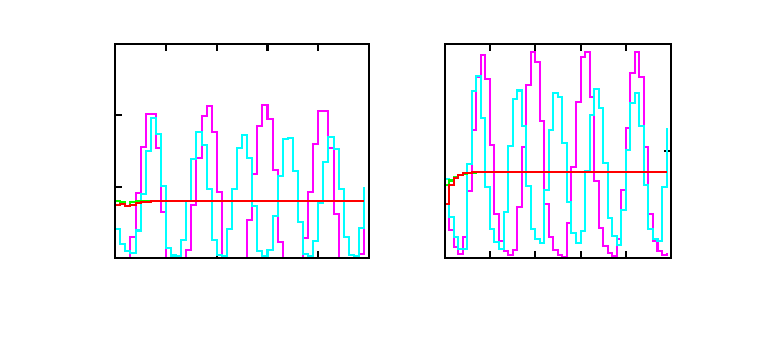
\includegraphics{sc/sS_demand_input}}%
    \gplfronttext
  \end{picture}%
\endgroup
}
% \caption{Open-loop prediction cost}
% \label{fig:sc:supplychain_example:lssc:VN}
% \end{figure}

\section{Discussion\footnote{This section, with the exception of the
    discussion about VMI appears in Section 6 of \citet{subramanian:rawlings:maravelias:2012}}}
\label{sec:sc:discussion}
\paragraph{Value of information:}
We observe that, for both order-up-to and inventory position control,
decentralized MPC produces large variations in the inventory and
orders. These variations indicate a large bullwhip effect, and
happen because the nodes have incomplete current information and no knowledge
of the dynamics of the other nodes. At each time step, the retailer 
assumes some flow of materials from the manufacturer to make inventory
predictions. Based on these predictions, the retailer places orders
with the manufacturer. Similarly, the manufacturer knows only the
current order quantity and  makes some assumptions about the future
orders from the retailer and makes production decisions. When
the actual orders and shipments arrive at the nodes, their decisions
are suboptimal.

Noncooperative MPC with the inventory position control policy  able
to reach a steady state, since, each node now has more information
about the ordering and production plans of the other node, both are able
to make better forecasts and therefore, better decisions.


\paragraph{Impact of ordering policy:}
In noncooperative MPC with inventory position control, we observe that
there are no inventory variations and the system reaches a
steady state. All flows through the system settle at the nominal
demand, which is the input steady state. The inventories, however,
show offset from the target. In order-up-to policy, irrespective of the
cost of placing large orders, the retailer is constrained to make
orders if the inventory at any period falls below the target.
In inventory position control, the orders placed are penalized, and therefore the retailer tends to order less, because the
optimizer tries to balance ordering costs and inventory deviation
costs. 

\paragraph{Plant-model mismatch:}
If we compare results for cooperative and centralized MPC with
noncooperative MPC, we see that, cooperative and centralized MPC reach
steady state more quickly. They achieve  steady state because there is no
information distortion in the system. Each node in cooperative
control,  optimizes not only the system-wide objective, it also
accounts for the dynamics of the entire supply chain. In noncooperative
MPC with inventory position control, since the retailer does not know the actual supply
chain dynamics, it settles at a steady state that depends on the inventory
position model. Therefore, we see the value of optimizing the actual dynamics instead
of introducing a mismatch between the models used by the controller
and the actual dynamics by using inventory position models. 

\paragraph{Guaranteed stability:}
The third important result of the analysis is that cooperative and
centralized MPC have been designed to guarantee closed-loop
stability. Although, we see that noncooperative MPC using inventory
position control has not made the supply chain unstable, we have no
stability guarantees. On the other hand, using the theory developed in
Section \ref{sec:mpc:distributed:coop}, we can guarantee closed-loop stability for
cooperative MPC.

\paragraph{Relation to echelon stock policies and VMI:}
Echelon stock policies are decentralized operating policies, but based
on the concept of echelon stock. Echelon stock is 
the stock carried by the node and all its downstream nodes. Therefore,
echelon stock based policies, to a certain extent, are like the
noncooperative MPC because the policies for a node depend on
information sharing regarding the inventories in all its downstream
node. 

Vendor managed inventory (VMI) is emerging as
a popular tool for supply chain integration. In VMI, the buyer
(retailer) authorizes the supplier (manufacturer) to maintain his
inventory. VMI, therefore resembles cooperative control because, not
only information regarding inventories is visible to the supplier, but
also the dynamics. The supplier, in a two-stage supply chain, manages
shipments between his facility and the retailer and production by
observing the retailer inventory. One of the main disadvantages of VMI
that has been reported is that the retailer loses control over
inventory management and some knowledge gained by the retailer (like
advanced forecasting) that could lead to better inventory management
cannot be used. Another disadvantage is that the overall supply chain
objective function is not used by the supplier \citep{sari:2007}. In this aspect, cooperative control can be seen as a
middle ground between VMI and decentralized control. In cooperative
control, each node still manages its own inventory, while optimizing
the overall supply chain objective function.

\newcommand{\bx}{\mathbf{x}}
\newcommand{\bd}{\mathbf{d}}


\chapter{Economic MPC for supply chains}
\label{chap:esc}
In this chapter, we propose an  economic model predictive
control (MPC) algorithm for inventory management in supply
chains with guaranteed closed-loop properties. We compare the
properties of the proposed controller with classical control policies
like the $(\sigma,\Sigma) $ policy. In the previous chapter, we showed
centralized and cooperative MPC designed to track the states of the
supply chain (inventories and backorders) to a steady state (target
stocks or safety stocks). The on-line optimization problem solved in
Chapter \ref{chap:sc} did not have any knowledge about the economics
of the process (\eg  cost of shipping, production etc.). Our focus in
this chapter is to leverage  recent developments in Economic-MPC
\citep{amrit:rawlings:angeli:2011,diehl:amrit:rawlings:2011} to
develop a stable controller for inventory management in which the
controller directly optimizes the supply chain economics. 

In Section \ref{sec:esc:economicMPC}, we review stability theory for economic
MPC and propose two flavors of MPC for a
supply chain, (i) a pure economic objective function and (ii) a mixed
objective comprising of an economic objective and a tracking
objective. We implement these economic MPC policies on the two stage
supply chain example introduced in Section
\ref{sec:sc:supplychain_example} . In Section
\ref{sec:esc:multi}, we implement the 
controller proposed in this chapter on a multi-product, multi-echelon
supply chain and compare the performance of the controller with that
of the $(\sigma,\Sigma) $ policy. In Section \ref{sec:esc:multi:scheduling}, we
introduce a scheduling model for the manufacturing facility with the
aim of integrating scheduling and inventory control using MPC. We
present results on recursive feasibility using ideas from
Chapter \ref{chap:scheduling}.


\section{Economic MPC theory}
\label{sec:esc:economicMPC}

As mentioned in Chapter \ref{chap:mpc}, the goal of controller design
using MPC is to stabilize the closed-loop. We show a supply chain
example to reinforce the idea that
simply solving an optimization problem at each sampling time in a
rolling horizon manner can destabilize the plant. 

Consider the two-stage supply chain example presented in Section
\ref{sec:sc:supplychain_example}. From equations
\eqref{eq:sc:scheduling_example:R} and \eqref{eq:sc:scheduling_example:M},
we can write the centralized supply chain model for the two node
system as:

\begin{multline}
\label{eq:esc:model0}
\underbrace{\begin{bmatrix}\Inv_1\\\BO_1\\\Inv_2 \\
    \BO_2\end{bmatrix}_{k+1}}_{x(k+1)} = 
\underbrace{\begin{bmatrix} 1 & & &
 \\ & 1 & &\\ & & 1 & \\ & & & 1\end{bmatrix}}_{A}
\underbrace{\begin{bmatrix}\Inv_1\\\BO_1\\\Inv_2 \\
    \BO_2\end{bmatrix}_{k}}_{x(k)}+
\underbrace{\begin{bmatrix}-1&0 &0 &0 \\-1&0 &0 &0 \\
0&0 & -1 &0 \\0 & 1 & -1 &0 \end{bmatrix}}_{B}
\underbrace{\begin{bmatrix}S_{1c}\\O_{12}\\S_{21}\\S_{2m}\end{bmatrix}_{k}}_{u(k)}+\\
\underbrace{\begin{bmatrix} 0&0 &1 &0 \\0 &0 &0 &0 \\
0&0 &0  &1 \\0 & 0 &0  &0 \end{bmatrix}}_{B^{(2)}}
\underbrace{\begin{bmatrix}S_{1c}\\O_{12}\\S_{21}\\S_{2m}\end{bmatrix}_{k-2}}_{u(k-2)}+
\underbrace{\begin{bmatrix}0 \\ 1 \\0 \\0 \end{bmatrix}}_{B_d}\underbrace{\begin{bmatrix}\Dem_{1c}\end{bmatrix}_{k}}_{d(k)}
\end{multline}

Using lifting and a slight abuse of notation, the supply chain model
can be written as:
\begin{equation}
\label{eq:esc:model}
x(k+1) = Ax(k) + Bu(k) + B_dd(k)
\end{equation}

We define the economic stage cost as
\begin{equation}
\label{eq:esc:ellE}
\ell_E(x,u) = q'x + r'u
\end{equation}
in which $q$ is a vector comprising of inventory holding $q_{\Inv_i}$
and lost sales $q_{\BO_i}$ costs, while $r$ is a vector comprising of
shipment costs $r_{S_{1c}}, r_{S_{21}}$,
production costs $r_{S_{2m}}$ and ordering costs $r_{O_{12}}$.

The stage cost defined in Chapter \ref{chap:mpc}, is the tracking
stage cost. In Chapter \ref{chap:mpc}, we defined the tracking cost to
track the state to the origin. In Chapter \ref{chap:sc}, we used
deviation variables $x \leftarrow x-x_s$ ($x_s$ being the
steady-state). In this chapter, we generalize the cost to track to a 
given target, and use absolute variables instead of tracking
variables. We (re)define the tracking stage cost as $\ell_T(x,u)$
given by:
\begin{equation}
\label{eq:esc:ellT}
\ell_T(x,u,z_p) = (x-x_t)'Q(x-x_t)+(u-u_t)'R(u-u_t)
\end{equation}
in which $z_p = (x_t',u_t')$ is a vector comprising of the state and
input targets $(x_t,u_t)$ respectively. The positive definite matrices
$Q,R$ penalize the deviation of the states and inputs from their
targets.

In order to ensure that the cooperative MPC problems in Chapter
\ref{chap:sc} converged to the centralized optimal solution, we used
Assumption \ref{ass:mpc:noX} to ``relax'' the
state constraints. Since, we only formulate centralized control
problems in this chapter, we re-introduce state constraints. The state
constraint is defined as 
\begin{equation}
\label{eq:esc:Xconst}
\mathbb{X}:= \set{x \mid \underbar{x} \leq x \leq \bar{x}}
\end{equation}

Similarly, the input constraint set is:
\begin{equation}
\label{eq:esc:Uconst}
\mathbb{U}:= \set{u \mid \underbar{u} \leq u \leq \bar{u}}
\end{equation}
The inequalities in \eqref{eq:esc:Xconst}, \eqref{eq:esc:Uconst} are componentwise. These
constraints define, for example, the positivity constraints for
backorders and inventories, capacities of the nodes, transportation
capacities etc.

Given a planning horizon $N$ and a demand forecast $\bd = 
(d(0),d(1),\ldots,d(N-1))$, we formulate the following
optimization problem:
\begin{alignat}{2}
\label{eq:esc:P}
\mathbb{P}_N(x):& \min_{\bu}{V_N(\bu;x,\bd,N)}& \nonumber \\
&\text{s.t.~} x(j+1) = Ax(j) + Bu(j)+B_dd(j),& j =\set{0,1,\ldots,N-1}\nonumber\\
&\underbar{x} \leq x(j) \leq \bar{x},& j = \set{0,1,\ldots,N}  \\
&\underbar{u} \leq u(j) \leq \bar{u},&j = \set{ 0,1,\ldots,N-1}\nonumber \\
& x(0) = x & \nonumber
\end{alignat}
in which $\bu = (u(0),u(1),\ldots,u(N-1))$. The cost function
$V_N(\bu;x,\bd,N)$ is the sum of $N$ stage costs
\[V_N(\bu;x,\bd,N) =  \sum_{i=0}^{N-1}
  \ell_E(x(i),u(i))\]
Notice that in Problem \eqref{eq:esc:P}, we do not have any terminal
penalty or constraints. In Figure \ref{fig:esc:unstable_SC}, we show
the backorder $\BO_1$ evolution for the retailer, for a controller
that solved problem \eqref{eq:esc:P} with $N=15$ and nominal demand
$d(k) =d_s= 10$. The stage cost was given by 
\[ q = (1,1,1,1)' \qquad r = (10,1,10,1)' \]
We assume that the shipping costs are greater than the backorder
costs. Clearly, we observe that despite implementing the optimal input at
each time instance, the backorder is increasing with time, indicating
that customer demand is not being met. Although, we have chosen a
pathological cost vector in which production costs are greater than
lost sales cost, we observe that there exists an unique steady-state
for this system $x_s = \underbar{x}=0, u_s = d_s$, that is the inventory
and backorders are zero and all the flows in the supply chain
(shipping and ordering between nodes, production) are equal to the
nominal demand.  The lower bounds on inventories and backorders are
zero. Notice that the choice of $u_s = d, x_s=0$ in \eqref{eq:esc:model}
is a solution to:
\[ (I-A)x -B^{(2)}u- Bu = B_dd \] 

Note that  the steady-state for the states in the supply
chain is independent of the demands and delays in the system.

For the costs mentioned
in above, staying at the steady-state incurs a cost of $220$ per period
which is much lesser than the cost incurred per period by the rolling
horizon controller, which is unbounded.

\begin{figure}
\centering
\scriptsize
\resizebox{\textwidth}{!}{% GNUPLOT: LaTeX picture with Postscript
\begingroup
  \makeatletter
  \providecommand\color[2][]{%
    \GenericError{(gnuplot) \space\space\space\@spaces}{%
      Package color not loaded in conjunction with
      terminal option `colourtext'%
    }{See the gnuplot documentation for explanation.%
    }{Either use 'blacktext' in gnuplot or load the package
      color.sty in LaTeX.}%
    \renewcommand\color[2][]{}%
  }%
  \providecommand\includegraphics[2][]{%
    \GenericError{(gnuplot) \space\space\space\@spaces}{%
      Package graphicx or graphics not loaded%
    }{See the gnuplot documentation for explanation.%
    }{The gnuplot epslatex terminal needs graphicx.sty or graphics.sty.}%
    \renewcommand\includegraphics[2][]{}%
  }%
  \providecommand\rotatebox[2]{#2}%
  \@ifundefined{ifGPcolor}{%
    \newif\ifGPcolor
    \GPcolortrue
  }{}%
  \@ifundefined{ifGPblacktext}{%
    \newif\ifGPblacktext
    \GPblacktexttrue
  }{}%
  % define a \g@addto@macro without @ in the name:
  \let\gplgaddtomacro\g@addto@macro
  % define empty templates for all commands taking text:
  \gdef\gplbacktext{}%
  \gdef\gplfronttext{}%
  \makeatother
  \ifGPblacktext
    % no textcolor at all
    \def\colorrgb#1{}%
    \def\colorgray#1{}%
  \else
    % gray or color?
    \ifGPcolor
      \def\colorrgb#1{\color[rgb]{#1}}%
      \def\colorgray#1{\color[gray]{#1}}%
      \expandafter\def\csname LTw\endcsname{\color{white}}%
      \expandafter\def\csname LTb\endcsname{\color{black}}%
      \expandafter\def\csname LTa\endcsname{\color{black}}%
      \expandafter\def\csname LT0\endcsname{\color[rgb]{1,0,0}}%
      \expandafter\def\csname LT1\endcsname{\color[rgb]{0,1,0}}%
      \expandafter\def\csname LT2\endcsname{\color[rgb]{0,0,1}}%
      \expandafter\def\csname LT3\endcsname{\color[rgb]{1,0,1}}%
      \expandafter\def\csname LT4\endcsname{\color[rgb]{0,1,1}}%
      \expandafter\def\csname LT5\endcsname{\color[rgb]{1,1,0}}%
      \expandafter\def\csname LT6\endcsname{\color[rgb]{0,0,0}}%
      \expandafter\def\csname LT7\endcsname{\color[rgb]{1,0.3,0}}%
      \expandafter\def\csname LT8\endcsname{\color[rgb]{0.5,0.5,0.5}}%
    \else
      % gray
      \def\colorrgb#1{\color{black}}%
      \def\colorgray#1{\color[gray]{#1}}%
      \expandafter\def\csname LTw\endcsname{\color{white}}%
      \expandafter\def\csname LTb\endcsname{\color{black}}%
      \expandafter\def\csname LTa\endcsname{\color{black}}%
      \expandafter\def\csname LT0\endcsname{\color{black}}%
      \expandafter\def\csname LT1\endcsname{\color{black}}%
      \expandafter\def\csname LT2\endcsname{\color{black}}%
      \expandafter\def\csname LT3\endcsname{\color{black}}%
      \expandafter\def\csname LT4\endcsname{\color{black}}%
      \expandafter\def\csname LT5\endcsname{\color{black}}%
      \expandafter\def\csname LT6\endcsname{\color{black}}%
      \expandafter\def\csname LT7\endcsname{\color{black}}%
      \expandafter\def\csname LT8\endcsname{\color{black}}%
    \fi
  \fi
  \setlength{\unitlength}{0.0500bp}%
  \begin{picture}(7200.00,3024.00)%
    \gplgaddtomacro\gplbacktext{%
      \csname LTb\endcsname%
      \put(1078,714){\makebox(0,0)[r]{\strut{} 0}}%
      \put(1078,970){\makebox(0,0)[r]{\strut{} 250}}%
      \put(1078,1225){\makebox(0,0)[r]{\strut{} 500}}%
      \put(1078,1481){\makebox(0,0)[r]{\strut{} 750}}%
      \put(1078,1737){\makebox(0,0)[r]{\strut{} 1000}}%
      \put(1078,1992){\makebox(0,0)[r]{\strut{} 1250}}%
      \put(1078,2248){\makebox(0,0)[r]{\strut{} 1500}}%
      \put(1078,2503){\makebox(0,0)[r]{\strut{} 1750}}%
      \put(1078,2759){\makebox(0,0)[r]{\strut{} 2000}}%
      \put(1210,484){\makebox(0,0){\strut{} 0}}%
      \put(2608,484){\makebox(0,0){\strut{} 50}}%
      \put(4007,484){\makebox(0,0){\strut{} 100}}%
      \put(5405,484){\makebox(0,0){\strut{} 150}}%
      \put(6803,484){\makebox(0,0){\strut{} 200}}%
      \put(176,1731){\rotatebox{-270}{\makebox(0,0){\strut{}Backorder -Retailer}}}%
      \put(4006,154){\makebox(0,0){\strut{}Time}}%
    }%
    \gplgaddtomacro\gplfronttext{%
    }%
    \gplbacktext
    \put(0,0){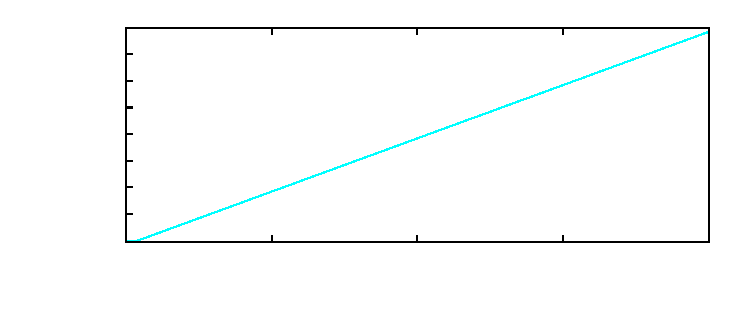
\includegraphics{esc/unstable_SC}}%
    \gplfronttext
  \end{picture}%
\endgroup
}
\caption{Backorder in the retailer for rolling horizon optimization
  without stability constraints.}
\label{fig:esc:unstable_SC}

\centering
\scriptsize
\resizebox{\textwidth}{!}{% GNUPLOT: LaTeX picture with Postscript
\begingroup
  \makeatletter
  \providecommand\color[2][]{%
    \GenericError{(gnuplot) \space\space\space\@spaces}{%
      Package color not loaded in conjunction with
      terminal option `colourtext'%
    }{See the gnuplot documentation for explanation.%
    }{Either use 'blacktext' in gnuplot or load the package
      color.sty in LaTeX.}%
    \renewcommand\color[2][]{}%
  }%
  \providecommand\includegraphics[2][]{%
    \GenericError{(gnuplot) \space\space\space\@spaces}{%
      Package graphicx or graphics not loaded%
    }{See the gnuplot documentation for explanation.%
    }{The gnuplot epslatex terminal needs graphicx.sty or graphics.sty.}%
    \renewcommand\includegraphics[2][]{}%
  }%
  \providecommand\rotatebox[2]{#2}%
  \@ifundefined{ifGPcolor}{%
    \newif\ifGPcolor
    \GPcolorfalse
  }{}%
  \@ifundefined{ifGPblacktext}{%
    \newif\ifGPblacktext
    \GPblacktexttrue
  }{}%
  % define a \g@addto@macro without @ in the name:
  \let\gplgaddtomacro\g@addto@macro
  % define empty templates for all commands taking text:
  \gdef\gplbacktext{}%
  \gdef\gplfronttext{}%
  \makeatother
  \ifGPblacktext
    % no textcolor at all
    \def\colorrgb#1{}%
    \def\colorgray#1{}%
  \else
    % gray or color?
    \ifGPcolor
      \def\colorrgb#1{\color[rgb]{#1}}%
      \def\colorgray#1{\color[gray]{#1}}%
      \expandafter\def\csname LTw\endcsname{\color{white}}%
      \expandafter\def\csname LTb\endcsname{\color{black}}%
      \expandafter\def\csname LTa\endcsname{\color{black}}%
      \expandafter\def\csname LT0\endcsname{\color[rgb]{1,0,0}}%
      \expandafter\def\csname LT1\endcsname{\color[rgb]{0,1,0}}%
      \expandafter\def\csname LT2\endcsname{\color[rgb]{0,0,1}}%
      \expandafter\def\csname LT3\endcsname{\color[rgb]{1,0,1}}%
      \expandafter\def\csname LT4\endcsname{\color[rgb]{0,1,1}}%
      \expandafter\def\csname LT5\endcsname{\color[rgb]{1,1,0}}%
      \expandafter\def\csname LT6\endcsname{\color[rgb]{0,0,0}}%
      \expandafter\def\csname LT7\endcsname{\color[rgb]{1,0.3,0}}%
      \expandafter\def\csname LT8\endcsname{\color[rgb]{0.5,0.5,0.5}}%
    \else
      % gray
      \def\colorrgb#1{\color{black}}%
      \def\colorgray#1{\color[gray]{#1}}%
      \expandafter\def\csname LTw\endcsname{\color{white}}%
      \expandafter\def\csname LTb\endcsname{\color{black}}%
      \expandafter\def\csname LTa\endcsname{\color{black}}%
      \expandafter\def\csname LT0\endcsname{\color{black}}%
      \expandafter\def\csname LT1\endcsname{\color{black}}%
      \expandafter\def\csname LT2\endcsname{\color{black}}%
      \expandafter\def\csname LT3\endcsname{\color{black}}%
      \expandafter\def\csname LT4\endcsname{\color{black}}%
      \expandafter\def\csname LT5\endcsname{\color{black}}%
      \expandafter\def\csname LT6\endcsname{\color{black}}%
      \expandafter\def\csname LT7\endcsname{\color{black}}%
      \expandafter\def\csname LT8\endcsname{\color{black}}%
    \fi
  \fi
  \setlength{\unitlength}{0.0500bp}%
  \begin{picture}(7200.00,3024.00)%
    \gplgaddtomacro\gplbacktext{%
      \csname LTb\endcsname%
      \put(814,832){\makebox(0,0)[r]{\strut{} 0}}%
      \put(814,1475){\makebox(0,0)[r]{\strut{} 10}}%
      \put(814,2117){\makebox(0,0)[r]{\strut{} 20}}%
      \put(814,2759){\makebox(0,0)[r]{\strut{} 30}}%
      \put(946,484){\makebox(0,0){\strut{} 0}}%
      \put(1433,484){\makebox(0,0){\strut{} 2}}%
      \put(1921,484){\makebox(0,0){\strut{} 4}}%
      \put(2408,484){\makebox(0,0){\strut{} 6}}%
      \put(2896,484){\makebox(0,0){\strut{} 8}}%
      \put(3383,484){\makebox(0,0){\strut{} 10}}%
      \put(176,1731){\rotatebox{-270}{\makebox(0,0){\strut{}Inventory}}}%
      \put(2164,154){\makebox(0,0){\strut{}Time}}%
    }%
    \gplgaddtomacro\gplfronttext{%
      \csname LTb\endcsname%
      \put(2061,2970){\makebox(0,0)[r]{\strut{}Retailer}}%
    }%
    \gplgaddtomacro\gplbacktext{%
      \csname LTb\endcsname%
      \put(4109,484){\makebox(0,0){\strut{} 0}}%
      \put(4544,484){\makebox(0,0){\strut{} 2}}%
      \put(4978,484){\makebox(0,0){\strut{} 4}}%
      \put(5413,484){\makebox(0,0){\strut{} 6}}%
      \put(5847,484){\makebox(0,0){\strut{} 8}}%
      \put(6282,484){\makebox(0,0){\strut{} 10}}%
      \put(6414,998){\makebox(0,0)[l]{\strut{} 0}}%
      \put(6414,2465){\makebox(0,0)[l]{\strut{} 10}}%
      \put(7051,1731){\rotatebox{-270}{\makebox(0,0){\strut{}Backorder}}}%
      \put(5195,154){\makebox(0,0){\strut{}Time}}%
    }%
    \gplgaddtomacro\gplfronttext{%
      \csname LTb\endcsname%
      \put(5039,2943){\makebox(0,0)[r]{\strut{}Manufacturer}}%
    }%
    \gplbacktext
    \put(0,0){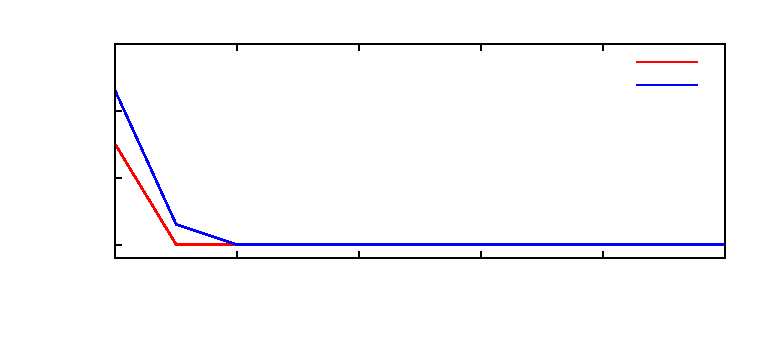
\includegraphics{stable_SC}}%
    \gplfronttext
  \end{picture}%
\endgroup
}
\caption{Closed loop evolution using stabilizing MPC.}
\label{fig:esc:stable_SC}

\end{figure}
For a simple two-node supply chain, we have demonstrated that simply
reoptimizing an economic objective function at each time instance
could lead to undesirable closed loop performance. Although, we chose
a pathological cost function to demonstrate the undesirable closed
loop, for a more complex supply chain, it is difficult to apriori
analyze all the interactions and judge if the rolling horizon
optimization will yield a desirable closed-loop. As mentioned in
Chapter \ref{chap:mpc}, stability theory for MPC gives us design
guidelines on the formulation of the on-line optimization problem, so that
closed-loop stability guarantees can be provided. While, we covered
tracking MPC stability theory in Chapter \ref{chap:mpc}, we briefly
review stability theory when the stage costs are economic (or other
general cost) functions. Stability theory for economic MPC is a
relatively new field \citep{diehl:amrit:rawlings:2011}
\citep{amrit:rawlings:angeli:2011}. We state the main results in this
chapter and refer the reader to the papers for more details. In
Chapter \ref{chap:mpc}, we ensured closed-loop properties by including
(i) a terminal cost $V_f(x)$ and (ii) a terminal region $x(N) \in
\mathbb{X}_f$. In the following sections, we outline the theory for economic MPC with terminal
equality constraint \citep{diehl:amrit:rawlings:2011}, i.e. $x(N) =
x_s$  and economic MPC with terminal penalty and region
\citep{amrit:rawlings:angeli:2011}.
 
\subsection{Terminal equality constraint formulation}
\label{sec:esc:terminal_equality}

We consider the system given by \eqref{eq:esc:model}. We consider the linear economic
cost given by \eqref{eq:esc:ellE}. The states are constrained to lie in
the hyperbox $\underbar{x} \leq x \leq \bar{x}$ while the inputs lie in
$\underbar{u} \leq u \leq \bar{u}$ (The inequalities are
componentwise). We assume that the sets 
\[\mathbb{X}: \set{x \mid \underbar{x} \leq x \leq  \bar{x}} \qquad \mathbb{U}: \set{u \mid \underbar{u} \leq u \leq \bar{u}}\] are
convex, bounded, closed, and contain the optimal steady-state defined later in
\eqref{eq:esc:SS}. Although many of the assumptions made in this chapter
are similar to the assumptions made for centralized MPC in Chapter
\ref{chap:mpc}, we reproduce them here again for clarity.

Note that the choice of linear models and cost function automatically satisfies Assumption \ref{ass:esc:cont}
stated below.

\begin{assumption}[Continuity]
\label{ass:esc:cont}
The system and the stage costs are  continuous.
\end{assumption}

We define the steady-state optimization problem as follows:

\begin{align}
\label{eq:esc:SS}
&\min_{x,u}{\ell_E(x,u;d_s)}  \nonumber \\
 &\text{s.t.~} x = Ax+Bu+B_dd_s, \\
&x \in \mathbb{X}, u \in \mathbb{U} \nonumber
\end{align}

We denote $(x_s,u_s;d_s)$ as the solution to \eqref{eq:esc:SS} and make the
following assumptions on $(x_s,u_s;d_s)$. The nominal demand is
denoted as $d_s$.

\begin{assumption}[Strict dissipativity]
\label{ass:esc:strict_dissipativity}
There exists $(x_s,u_s;d_s)$ and $\lambda_s$ so that 
\begin{enumerate}[(a)]
\item $(x_s,u_s;d_s)$  is an unique solution of \eqref{eq:esc:SS}.
\item The multiplier $\lambda_s$ is such that $(x_s,u_s;d_s)$
  uniquely solves \eqref{eq:esc:SS1}
\begin{equation}
\label{eq:esc:SS1}
\min_{x,u}{\ell_E(x,u)+\lambda_s'[x-(Ax+Bu+B_dd_s)]} \quad \text{s.t.~}
  x \in \mathbb{X}, u \in \mathbb{U}
\end{equation}
\item The system $x^+=Ax+Bu+B_dd_s$ is strictly dissipative with respect
  to the supply rate $s(x,u) = \ell_E(x,u)-\ell_E(x_s,u_s)$ and
  storage function $\lambda(x) = \lambda_s'x$. That is, there exists a
  $\mathcal{K}_{\infty}$ function $\rho(\cdot)$ such that:
\begin{equation}
\label{eq:esc:strict_dissipativity}
\lambda_s'(Ax+Bu+B_dd_s-x) \leq -\rho (x-x_s)+s(x,u), \forall (x,u) \in
\mathbb{X} \times \mathbb{U}
\end{equation}
\end{enumerate}
\end{assumption}


Because of the structure of the state space matrix $A$ in \eqref{eq:esc:model0}-\eqref{eq:esc:model}, the steady-state
problem \eqref{eq:esc:SS} decomposes into two problems:
\begin{equation}
\label{eq:esc:SSx} \min_{x}{q'x} \qquad \text{s.t.~} \underbar{x} \leq x
\leq \bar{x}
\end{equation}
and
\begin{equation}
\label{eq:esc:SSu} \min_{u}{r'u} \qquad \text{s.t.~} B^{(1)}u + B^{(2)}u +
Bu + B_dd_s = 0,
 \underbar{u} \leq u\leq \bar{u}
\end{equation}

By choosing $\lambda_s$
as the optimal Lagrange multiplier for the equality constraints in
\eqref{eq:esc:SS}, we can establish that the $(x_s,u_s;d_s)$ is the unique
solution of optimization problem \eqref{eq:esc:SS1}. 

Hence Assumption \ref{ass:esc:strict_dissipativity} is satisfied by the
supply chain model.

We now define the terminal equality constraint MPC optimization
problem:
\begin{alignat}{2}
\label{eq:esc:PT}
\mathbb{P}_N(x):& \min_{\bu}{V_N(\bu;x,\bd,N)}& \nonumber \\
&\text{s.t.~} x(j+1) = Ax(j) + Bu(j)+B_dd(j),& j =\set{0,1,\ldots,N-1}\nonumber\\
&\underbar{x} \leq x(j) \leq \bar{x},& j =  \set{0,1,\ldots,N}  \\
&\underbar{u} \leq u(j) \leq \bar{u},&j = \set{0,1,\ldots,N-1}
\nonumber\\
&x(0) = x & \nonumber \\
&x(N) = x_s & \label{eq:esc:PT:xN}
\end{alignat}
in which $\bu = (u(0),u(1),\ldots,u(N-1))$. The cost function
$V_N(\bu;x,\bd,N)$ is the sum of $N$ stage costs
\[V_N(\bu;x,\bd,N) =  \sum_{i=0}^{N-1}
  \ell_E(x(i),u(i))\]

Note that in contrast to problem \eqref{eq:esc:P},
we have added a terminal constraint that $x(N) = x_s$ in problem
\eqref{eq:esc:PT}. The steady state $x_s$ is the solution to the
optimization problem \eqref{eq:esc:SS}.

Before presenting the stability theorem, attributed to
\citet{diehl:amrit:rawlings:2011}, we define the following sets and
the control law.

The set of admissible state-input pairs $(x,\bu)$ is denoted by
$\mathbb{Z}_T$ as follows (see  definition  \eqref{eq:mpc:Z}):
\begin{equation}
\mathbb{Z}_T := \left \lbrace(x,\bu) \mid \phi(i;x,\bu,\bd_s) \in
  \mathbb{X} \right . ,\\ \left . \bu \in \mathbb{U}^N, \phi(N;x,\bu,\bd_s) = x_s\right\rbrace
\end{equation}
in which $\bd_s$ is the nominal demand vector and
$\phi(i;x,\bu,\bd_s)$ denotes the solution at time $i$ under input
$\bu$ starting from $x$ at time $0$. 

The projection of set $\mathbb{Z}_T$ onto the feasible state space
$\mathbb{X}$ is called the set of admissible initial states,
$\mathcal{X}_{N,T}$ (see definition \eqref{eq:mpc:X_N})

\begin{equation}
\mathcal{X}_{N,T} := \set{x \mid \exists \bu \in \mathbb{U}^N
  \text{s.t.~} (x,\bu) \in \mathbb{Z}_T}
\end{equation}

We denote the optimal solution of problem \eqref{eq:esc:PT} as
$\bu^0(x(k),\bd_s)$. Denoting the first input in the sequence
$\bu^0(x(k),\bd_s)$ as $\kappa_T(x(k))$, we obtain the closed-loop
dynamics of the MPC algorithm as $x^+ = Ax+B\kappa_T(x)+B_dd_s$.  The
control law is $\kappa_T(x(k))$. Note that, similar to nominal MPC, we
prove the closed-loop properties for economic MPC only for the nominal
demand $d_s$.

%We also make the following assumption because we require some form of
%system controllability
%\begin{assumption}[Weak Controllability]
%\label{ass:weak_controllability}
%There exists a $\mathcal{K}_\infty$ function $\gamma(\cdot)$ such that
%for every $x \in \mathcal{X}_{N,T}$, there exists $\bu$ such that
%$(x,\bu) \in \mathbb{Z}_T$ and 
%\begin{equation}
%\label{eq:esc:weak_controllability}
%\sum_{i=0}^{N-1} \norm{u_i-u_s} \leq \gamma(\norm{x-x_s})
%\end{equation}
%\end{assumption}

%Note that Assumption \ref{ass:weak_controllability} is satisfied by
%linear stabilizable systems. Hence, it is satisfied for the supply
%chain model.

\begin{theorem}[Lyapunov function with terminal equality constraint]
\label{thm:esc:EqualityConstraint}
Let Assumptions \ref{ass:mpc:stab}, \ref{ass:esc:cont} -- \ref{ass:esc:strict_dissipativity}
hold. Then the steady-state solution of the closed-loop system $x^+ =
Ax+B\kappa_T(x)+B_dd_s$ is asymptotically stable with
$\mathcal{X}_{N,T}$ as the region of attraction. The Lyapunov function
is
\[ \tilde{V}(x) := V_N(x) +\lambda_s'[x-x_s]-N\ell_E(x_s,u_s) \]
\end{theorem}
 
Theorem \ref{thm:esc:EqualityConstraint} allows us to conclude that
rolling horizon optimization in which we solve optimization problem
\eqref{eq:esc:PT} at each sampling instance steers any initial state
$x(0) \in \mathcal{X}_{N,T}$ to the steady-state $x_s$. Therefore, in
contrast to the closed-loop observed in Figure \ref{fig:esc:unstable_SC},
a controller optimizing \eqref{eq:esc:PT} would have never
left the steady-state, thereby only incurring a cost of $220$ per
period. In Figure \ref{fig:esc:stable_SC}, we plot the closed-loop for a
$x(0) \neq x_s$ (using the same cost vector used in the previous
section).




Although economic MPC with terminal equality constraints stabilizes
the supply chain system, notice that the unique steady-state for the
states that is obtained by solving the linear program \eqref{eq:esc:SSx}
is on one of the vertices of the hyperbox $\mathbb{X}$. More
importantly, since the cost vector $q$ is composed of inventory
holding and lost sales costs, all its elements are strictly
positive. Therefore, the solution of \eqref{eq:esc:SSx} is $x_s =
\underbar{x}$. This steady state value of the state variables has
important implications which motivates us to formulate the
multiobjective supply chain MPC with terminal region in the next
section. It is important to note that (i) $\mathcal{X}_{N,T}$
comprises of $x \geq \underbar{x}$ and (ii) since the steady state
does not lie in the interior of $\mathbb{X}$, we cannot use the
terminal penalty/ region formulation that is discussed in the next
section to stabilize economic MPC.

Supply chain managers often balance economic objectives with that of
risk minimization. That is, in addition to minimizing costs (or
maximizing profits), the manager also tries to minimize risk by
maintaining or by tracking inventory around a  safety-stock level
(that could determined by minimizing the probability of stock-out
etc. or is the solution of stochastic inventory control algorithms
like \citet{federgruen:1993, shang:song:2003, dong:lee:2003,
  gallego:ozer:2005,chen:song:2001}). As we stated above, stabilizing
economic-MPC can only stabilize $x_s = \underbar{x}$. Therefore, to
incorporate the managers choice to track safety stocks, we introduce
a tracking stage cost \eqref{eq:esc:ellT}
and minimize a combined economic and tracking objective in the next section.

\subsection{Terminal region formulation}
In order to allow the practitioner to implement
a controller that tracks inventories to a steady-state as well as
optimize the economics of the system, we use the following stage cost,
\begin{equation}
\label{eq:esc:ell}
\ell(x,u) = \frac{\omega}{s_E} \ell_E(x,u) + \frac{(1-\omega)}{s_T} \ell_T(x,u;z_p)
\end{equation}
in which $\omega \in (0,1)$ is a relative weighting chosen by the
practitioner between the tracking and the economic stage costs. We use
the parameters $Q,R$ in $\ell_T(x,u)$ and $\omega$ as tuning
parameters for the multiobjective MPC controller. The parameters
$(s_E,s_T)$ are scaling constants while $z_p=(x_t,u_t)$ are the tracking
set-points.

We choose the input target $u_t$ to be the ``economic'' input that
satisfies the nominal demand, that is $u_t = u_s$ in which $u_s$ is
the solution to \eqref{eq:esc:SSu}. The target set-point for the states is
$x_t = x_{\text{safety}}$. The steady-state optimization problem
now becomes
\begin{align}
\label{eq:esc:SSMulti}
&\min_{x,u}{}(\frac{\omega}{s_E} (q'x+r'u) +
\frac{(1-\omega)}{s_T}((x-x_{\text{safety}})'Q(x-x_{\text{safety}})+(u-u_s)'R(u-u_s)))
\nonumber\\
&\text{s.t.~} x=Ax+Bu+B_dd_s, u \in \mathbb{U}, x \in \mathbb{X} 
\end{align}

To obtain the scaling parameters $s_T,s_E$, we consider the utopia and
nadir points of the individual stage costs $\ell_E(x,u)$ and
$\ell_T(x,u;z_p)$ \citep{kim:weck:2005}. Denoting $z = (x,u)$, we obtain
\[ z_E = \text{arg}\min_{z \in \mathbb{X} \times
  \mathbb{U}}{\ell_E(x,u)}, \quad z_T = \text{arg}\min_{z \in \mathbb{X} \times
  \mathbb{U}}{\ell_T(x,u;z_p)} \]
The utopia point is \[J^U = (\ell_E(z_E),\ell_T(z_T;z_p))\in
\mathbb{R}^2\] 
The nadir point is \[J^N = (\ell_E(z_T),\ell_T(z_E;z_p))\in
\mathbb{R}^2 \] 
The parameters $s_T,s_E$ are then defined as:
\[ (s_E,s_T) = J^N-J^U \]

Note that  the optimization problem \eqref{eq:esc:SSMulti} is a quadratic program with a positive
definite Hessian, and hence an unique solution to \eqref{eq:esc:SSMulti}
exists.
Based on the choice $\omega$ and
tuning parameters $(Q,R)$, the MPC controller described in this section stabilizes a different
$x_s$. That is, the choice of weighting given to the economic and
tracking objectives decide what inventories the controller is going to stabilize.


In Figure \ref{fig:esc:SS_omega}, we plot the inventory steady-state as a
function of $\omega$. The parameters used are $ Q =
10\diag{(1,1,1,1)}, R = 10^{-5}\diag{(1,1,1,1)}$, $x_{\text{safety}}
= (35,0,40,0)$. The economic costs are $q = (10,10,10,1), r =
(10,0.1,10,100)$. The input and state constraints were chosen as
\[ 0 \leq x \leq 100 \qquad 0 \leq u \leq 20 \]
The nominal demand
$d_s$ was $10$. Note that by choice of the state targets,the
steady-state backorders at both nodes is zero.

\begin{figure}[h]
\centering
\scriptsize
\resizebox{\textwidth}{!}{% GNUPLOT: LaTeX picture with Postscript
\begingroup
  \makeatletter
  \providecommand\color[2][]{%
    \GenericError{(gnuplot) \space\space\space\@spaces}{%
      Package color not loaded in conjunction with
      terminal option `colourtext'%
    }{See the gnuplot documentation for explanation.%
    }{Either use 'blacktext' in gnuplot or load the package
      color.sty in LaTeX.}%
    \renewcommand\color[2][]{}%
  }%
  \providecommand\includegraphics[2][]{%
    \GenericError{(gnuplot) \space\space\space\@spaces}{%
      Package graphicx or graphics not loaded%
    }{See the gnuplot documentation for explanation.%
    }{The gnuplot epslatex terminal needs graphicx.sty or graphics.sty.}%
    \renewcommand\includegraphics[2][]{}%
  }%
  \providecommand\rotatebox[2]{#2}%
  \@ifundefined{ifGPcolor}{%
    \newif\ifGPcolor
    \GPcolortrue
  }{}%
  \@ifundefined{ifGPblacktext}{%
    \newif\ifGPblacktext
    \GPblacktexttrue
  }{}%
  % define a \g@addto@macro without @ in the name:
  \let\gplgaddtomacro\g@addto@macro
  % define empty templates for all commands taking text:
  \gdef\gplbacktext{}%
  \gdef\gplfronttext{}%
  \makeatother
  \ifGPblacktext
    % no textcolor at all
    \def\colorrgb#1{}%
    \def\colorgray#1{}%
  \else
    % gray or color?
    \ifGPcolor
      \def\colorrgb#1{\color[rgb]{#1}}%
      \def\colorgray#1{\color[gray]{#1}}%
      \expandafter\def\csname LTw\endcsname{\color{white}}%
      \expandafter\def\csname LTb\endcsname{\color{black}}%
      \expandafter\def\csname LTa\endcsname{\color{black}}%
      \expandafter\def\csname LT0\endcsname{\color[rgb]{1,0,0}}%
      \expandafter\def\csname LT1\endcsname{\color[rgb]{0,1,0}}%
      \expandafter\def\csname LT2\endcsname{\color[rgb]{0,0,1}}%
      \expandafter\def\csname LT3\endcsname{\color[rgb]{1,0,1}}%
      \expandafter\def\csname LT4\endcsname{\color[rgb]{0,1,1}}%
      \expandafter\def\csname LT5\endcsname{\color[rgb]{1,1,0}}%
      \expandafter\def\csname LT6\endcsname{\color[rgb]{0,0,0}}%
      \expandafter\def\csname LT7\endcsname{\color[rgb]{1,0.3,0}}%
      \expandafter\def\csname LT8\endcsname{\color[rgb]{0.5,0.5,0.5}}%
    \else
      % gray
      \def\colorrgb#1{\color{black}}%
      \def\colorgray#1{\color[gray]{#1}}%
      \expandafter\def\csname LTw\endcsname{\color{white}}%
      \expandafter\def\csname LTb\endcsname{\color{black}}%
      \expandafter\def\csname LTa\endcsname{\color{black}}%
      \expandafter\def\csname LT0\endcsname{\color{black}}%
      \expandafter\def\csname LT1\endcsname{\color{black}}%
      \expandafter\def\csname LT2\endcsname{\color{black}}%
      \expandafter\def\csname LT3\endcsname{\color{black}}%
      \expandafter\def\csname LT4\endcsname{\color{black}}%
      \expandafter\def\csname LT5\endcsname{\color{black}}%
      \expandafter\def\csname LT6\endcsname{\color{black}}%
      \expandafter\def\csname LT7\endcsname{\color{black}}%
      \expandafter\def\csname LT8\endcsname{\color{black}}%
    \fi
  \fi
  \setlength{\unitlength}{0.0500bp}%
  \begin{picture}(7200.00,3024.00)%
    \gplgaddtomacro\gplbacktext{%
      \csname LTb\endcsname%
      \put(814,802){\makebox(0,0)[r]{\strut{} 0}}%
      \put(814,1291){\makebox(0,0)[r]{\strut{} 10}}%
      \put(814,1780){\makebox(0,0)[r]{\strut{} 20}}%
      \put(814,2270){\makebox(0,0)[r]{\strut{} 30}}%
      \put(814,2759){\makebox(0,0)[r]{\strut{} 40}}%
      \put(946,484){\makebox(0,0){\strut{} 0}}%
      \put(3383,484){\makebox(0,0){\strut{} 1}}%
      \put(176,1731){\rotatebox{-270}{\makebox(0,0){\strut{}Inventory}}}%
      \put(2164,154){\makebox(0,0){\strut{}$\omega$}}%
    }%
    \gplgaddtomacro\gplfronttext{%
      \csname LTb\endcsname%
      \put(2396,2586){\makebox(0,0)[r]{\strut{}Retailer}}%
    }%
    \gplgaddtomacro\gplbacktext{%
      \csname LTb\endcsname%
      \put(4109,484){\makebox(0,0){\strut{} 0}}%
      \put(6282,484){\makebox(0,0){\strut{} 1}}%
      \put(6414,791){\makebox(0,0)[l]{\strut{} 0}}%
      \put(6414,1229){\makebox(0,0)[l]{\strut{} 10}}%
      \put(6414,1666){\makebox(0,0)[l]{\strut{} 20}}%
      \put(6414,2103){\makebox(0,0)[l]{\strut{} 30}}%
      \put(6414,2540){\makebox(0,0)[l]{\strut{} 40}}%
      \put(7051,1731){\rotatebox{-270}{\makebox(0,0){\strut{}Inventory}}}%
      \put(5195,154){\makebox(0,0){\strut{}$\omega$}}%
    }%
    \gplgaddtomacro\gplfronttext{%
      \csname LTb\endcsname%
      \put(5295,2586){\makebox(0,0)[r]{\strut{}Manufacturer}}%
    }%
    \gplbacktext
    \put(0,0){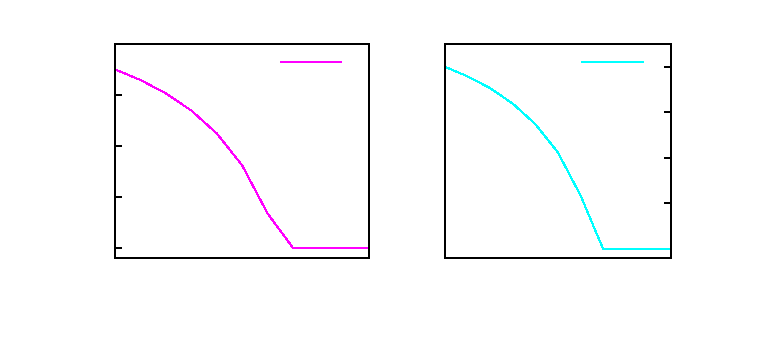
\includegraphics{esc/SS_omega}}%
    \gplfronttext
  \end{picture}%
\endgroup
}
\caption{Steady-state as a function of the relative weighting between tracking and
  economics}
\label{fig:esc:SS_omega}
\end{figure}

Figure \ref{fig:esc:SS_omega} shows the trade-off between choosing to
rack to the safety stock and choosing to minimize the economics. As
the economic weight increases, we see that the steady-state
approaches the economic steady state.

\paragraph{Terminal region and Terminal penalty.}
Let  Assumptions \ref{ass:esc:cont} and
\ref{ass:esc:strict_dissipativity}(a) and
\ref{ass:esc:strict_dissipativity}(c) hold. In Assumption
\ref{ass:esc:strict_dissipativity}, we use $\ell(x,u)-\ell(x_s,u_s)$ in
which $\ell(x,u)$ is given by \eqref{eq:esc:ell} and $(x_s,u_s)$ is the
solution of the steady-state problem \eqref{eq:esc:SSMulti} as the storage
function. In addition, we make the basic stability assumption
\ref{eq:mpc:bsa}; with modifications to accommodate an economic stage
cost as:

\begin{assumption}[Basic stability assumption]
\label{ass:esc:bsa}
There exists a convex, compact terminal region $\mathbb{X}_f \subseteq
\mathbb{X}$, containing the point $x_s$ in its interior and a control
law $\kappa_f: \mathbb{X}_f \rightarrow \mathbb{U}$  and a function
$V_f:\mathbb{X}_f \rightarrow \mathbb{R}$ such that the
following holds
\begin{align}
\label{eq:esc:BSA}
V_f(Ax+B\kappa_f(x)+B_dd_s) \leq V_f(x)-\ell(x,\kappa_f(x))+\ell(x_s,u_s),&\forall x \in \mathbb{X}_f  \\
\label{eq:esc:invariant}
Ax+ B\kappa_f(x) +B_dd_s \in \mathbb{X}_f&,\forall x \in \mathbb{X}_f 
\end{align}
\end{assumption}

We now define the terminal penalty MPC problem:
\begin{alignat}{2}
\label{eq:esc:PP}
\mathbb{P}_N(x):& \min_{\bu}{V_N(\bu;x,\bd,N)}& \nonumber \\
&\text{s.t.~} x(j+1) = Ax(j) + Bu(j)+B_dd(j),& j = \set{0,1,\ldots,N-1}\nonumber\\
&\underbar{x} \leq x(j) \leq \bar{x},& j = \set{0,1,\ldots,N}  \\
&\underbar{u} \leq u(j) \leq \bar{u},&j = \set{0,1,\ldots,N-1}
\nonumber\\
&x(0) = x & \nonumber \\
&x(N) \in \mathbb{X}_f & \nonumber %\label{eq:esc:PP:xN}
\end{alignat}
in which $V_N(\bu;x,\bd,N) = \sum_{i=0}^{N-1}
\ell(x(i),u(i))+ V_f(x(N))$.


Analogous to $\mathbb{Z}_T$ and $\mathcal{X}_{N,T}$, we define the
sets $\mathbb{Z}_P$ and $\mathbb{X}_{N,P}$ (the subscript $P$ refers
to terminal penalty) as follows:
\[ \mathbb{Z}_P := \set{(x,\bu) \mid  \bu \in \mathbb{U}^N,
 \phi(i;x,\bu,\bd_s) \in \mathbb{X},  \phi(N;x,\bu,\bd_s) \in \mathbb{X}_f}\]
in which $\bd_s$ is the nominal demand vector and
$\phi(i;x,\bu,\bd_s)$ denotes the solution at time $i$ under input
$\bu$ starting from $x$ at time $0$. 

The projection of set $\mathbb{Z}_P$ onto the feasible state space
$\mathbb{X}$ is called the set of admissible initial states,
$\mathcal{X}_{N,P}$

\[\mathcal{X}_{N,P} := \set{x \mid \exists \bu \in \mathbb{U}^N
  \text{s.t.~} (x,\bu) \in \mathbb{Z}_P} \]

We denote the optimal solution of problem \eqref{eq:esc:PP} as
$\bu^0(x(k),\bd_s)$. Denoting the first input in the sequence
$\bu^0(x(k),\bd_s)$ as $\kappa_P(x(k))$, we obtain the closed-loop
dynamics of the MPC algorithm as $x^+ = Ax+B\kappa_P(x)+B_dd_s$.  The
control law is $\kappa_P(x(k))$.

To show that the closed-loop using the control law $u = \kappa_P(x)$
is asymptotically stable, we need to make the following  assumption:

\begin{assumption}[Continuity of the storage function]
\label{ass:esc:cont_lambda}
The storage function $\lambda(\cdot)$ is continuous on $\mathbb{X}
\times  \mathbb{U}$
\end{assumption}

The following theorem attributed to \citet{amrit:rawlings:angeli:2011}
establishes that the closed-loop $x^+ = Ax+B\kappa_P(x)+B_dd_s$ is
asymptotically stable.

\begin{theorem}[Lyapunov stability with terminal region]
Let Assumptions \ref{ass:esc:cont}, \ref{ass:esc:strict_dissipativity}(a),
\ref{ass:esc:strict_dissipativity}(c), \ref{ass:esc:bsa} and
\ref{ass:esc:cont_lambda} hold. Then the steady-state solution $x_s$ is an
asymptotically stable equilibrium point of the system
$x^+=Ax+B\kappa_P(x)+B_dd_s$ with the region of attraction being any
arbitrarily large compact subset of $\mathcal{X}_{N,P}$. The Lyapunov
function is 
\begin{equation*}
\bar{V}_N^0(\bu;x(k),\bd_s) =
V_N^0(\bu;x(k),\bd_s)-N\ell(x_s,u_s)-\lambda(x_s)-V_f(x_s)
\end{equation*}
in which $V_N^0(\bu;x(k),\bd_s)$ is the optimal value function in the solution
of problem \eqref{eq:esc:PP}.
\end{theorem}

We now discuss the choice of terminal region and terminal penalty for
the supply chain model. Note that the optimal Lagrange multiplier for
the equality constraints in steady-state problem \eqref{eq:esc:SSMulti}
satisfies all the requirements in Assumptions
\ref{ass:esc:strict_dissipativity} and \ref{ass:esc:cont_lambda}. 

For the supply chain model, we choose the terminal controller
$\kappa_f(x) = Kx$, in which the gain $K$ is such that $A_K :=A+BK$ is
a Hurwitz. That is, the system $\tilde{x}^+ = A_K\tilde{x}$ is
asymptotically stable with the equilibrium point being $x_s$, in
which $\tilde{x}$ is the deviation variable $x-x_s$. Note that the
input is $\tilde{u} = K\tilde{x}$.  Since the supply
chain model $(A,B)$ is stabilizable, such an $K$ exists (for example,
the infinite horizon unconstrained LQR gain). By the choice
$\underbar{x} = 0$  and backorder targets, some state constraints are
active at the steady state. Hence,  we find $K$ using the technique given by
\citet{rao:rawlings:1999}. By this choice of the controller gain, we
restrict the evolution of the closed-loop $(A+BK)\tilde{x}$ to the
null space of the active constraints at the origin (the steady state
is shifted to the origin in deviation variables). We define $Q_K = Q+K'RK$
and $q_K = q+K'r$. We choose the terminal penalty to be 
\begin{equation}
\label{eq:esc:Vf}
V_f(x;x_s) = (x-x_s)'P(x-x_s)+ p'(x-x_s)
\end{equation}

in which the positive definite matrix $P$ is the solution to the
Lyapunov equation
\[ A_K'PA_K-P = -Q_K \]
and $p$ is the solution to 
\[ (A_K-I)'p = -q_K \]

In order that the basic stability assumption be satisfied, we require
that  
\begin{equation}
\label{eq:esc:BSA_condition}
(x-x_s)'Q(x_s-x_t)  \leq 0
\end{equation}


Therefore, we construct the terminal region $\mathbb{X}_f$ as the
following set:
\begin{equation}
\label{eq:esc:Xf}
\mathbb{X}_f := \left \lbrace x \mid A_Kx+Bu_s+B_dd_s \in
  \mathbb{X}_f,  K(x-x_s)+u_s \in \mathbb{U}, (x-x_s)'Q(x_s-x_t) \leq 0\right \rbrace
\end{equation}

Such a set can be constructed using the maximal output admissible set
algorithm presented in \citet{gilbert:tan:1991} or by using the
efficient algorithms presented in the MPT toolbox
\citep{kvasnica:grieder:baotic:2006}. In Figure \ref{fig:esc:Xf4}, we plot
the projection of the terminal region on the $\Inv_1-\Inv_2$
plane. The cost functions and constraints were the same as in the
steady-state calculation. The parameter $\omega$ is chosen to be
$0.4$.

\begin{figure}
\centering
\scriptsize
\resizebox{0.75\textwidth}{!}{% GNUPLOT: LaTeX picture with Postscript
\begingroup
  \makeatletter
  \providecommand\color[2][]{%
    \GenericError{(gnuplot) \space\space\space\@spaces}{%
      Package color not loaded in conjunction with
      terminal option `colourtext'%
    }{See the gnuplot documentation for explanation.%
    }{Either use 'blacktext' in gnuplot or load the package
      color.sty in LaTeX.}%
    \renewcommand\color[2][]{}%
  }%
  \providecommand\includegraphics[2][]{%
    \GenericError{(gnuplot) \space\space\space\@spaces}{%
      Package graphicx or graphics not loaded%
    }{See the gnuplot documentation for explanation.%
    }{The gnuplot epslatex terminal needs graphicx.sty or graphics.sty.}%
    \renewcommand\includegraphics[2][]{}%
  }%
  \providecommand\rotatebox[2]{#2}%
  \@ifundefined{ifGPcolor}{%
    \newif\ifGPcolor
    \GPcolortrue
  }{}%
  \@ifundefined{ifGPblacktext}{%
    \newif\ifGPblacktext
    \GPblacktexttrue
  }{}%
  % define a \g@addto@macro without @ in the name:
  \let\gplgaddtomacro\g@addto@macro
  % define empty templates for all commands taking text:
  \gdef\gplbacktext{}%
  \gdef\gplfronttext{}%
  \makeatother
  \ifGPblacktext
    % no textcolor at all
    \def\colorrgb#1{}%
    \def\colorgray#1{}%
  \else
    % gray or color?
    \ifGPcolor
      \def\colorrgb#1{\color[rgb]{#1}}%
      \def\colorgray#1{\color[gray]{#1}}%
      \expandafter\def\csname LTw\endcsname{\color{white}}%
      \expandafter\def\csname LTb\endcsname{\color{black}}%
      \expandafter\def\csname LTa\endcsname{\color{black}}%
      \expandafter\def\csname LT0\endcsname{\color[rgb]{1,0,0}}%
      \expandafter\def\csname LT1\endcsname{\color[rgb]{0,1,0}}%
      \expandafter\def\csname LT2\endcsname{\color[rgb]{0,0,1}}%
      \expandafter\def\csname LT3\endcsname{\color[rgb]{1,0,1}}%
      \expandafter\def\csname LT4\endcsname{\color[rgb]{0,1,1}}%
      \expandafter\def\csname LT5\endcsname{\color[rgb]{1,1,0}}%
      \expandafter\def\csname LT6\endcsname{\color[rgb]{0,0,0}}%
      \expandafter\def\csname LT7\endcsname{\color[rgb]{1,0.3,0}}%
      \expandafter\def\csname LT8\endcsname{\color[rgb]{0.5,0.5,0.5}}%
    \else
      % gray
      \def\colorrgb#1{\color{black}}%
      \def\colorgray#1{\color[gray]{#1}}%
      \expandafter\def\csname LTw\endcsname{\color{white}}%
      \expandafter\def\csname LTb\endcsname{\color{black}}%
      \expandafter\def\csname LTa\endcsname{\color{black}}%
      \expandafter\def\csname LT0\endcsname{\color{black}}%
      \expandafter\def\csname LT1\endcsname{\color{black}}%
      \expandafter\def\csname LT2\endcsname{\color{black}}%
      \expandafter\def\csname LT3\endcsname{\color{black}}%
      \expandafter\def\csname LT4\endcsname{\color{black}}%
      \expandafter\def\csname LT5\endcsname{\color{black}}%
      \expandafter\def\csname LT6\endcsname{\color{black}}%
      \expandafter\def\csname LT7\endcsname{\color{black}}%
      \expandafter\def\csname LT8\endcsname{\color{black}}%
    \fi
  \fi
  \setlength{\unitlength}{0.0500bp}%
  \begin{picture}(7200.00,5040.00)%
    \gplgaddtomacro\gplbacktext{%
      \csname LTb\endcsname%
      \put(814,704){\makebox(0,0)[r]{\strut{} 0}}%
      \put(814,1383){\makebox(0,0)[r]{\strut{} 10}}%
      \put(814,2061){\makebox(0,0)[r]{\strut{} 20}}%
      \put(814,2740){\makebox(0,0)[r]{\strut{} 30}}%
      \put(814,3418){\makebox(0,0)[r]{\strut{} 40}}%
      \put(814,4097){\makebox(0,0)[r]{\strut{} 50}}%
      \put(814,4775){\makebox(0,0)[r]{\strut{} 60}}%
      \put(946,484){\makebox(0,0){\strut{} 0}}%
      \put(1678,484){\makebox(0,0){\strut{} 10}}%
      \put(2410,484){\makebox(0,0){\strut{} 20}}%
      \put(3142,484){\makebox(0,0){\strut{} 30}}%
      \put(3875,484){\makebox(0,0){\strut{} 40}}%
      \put(4607,484){\makebox(0,0){\strut{} 50}}%
      \put(5339,484){\makebox(0,0){\strut{} 60}}%
      \put(6071,484){\makebox(0,0){\strut{} 70}}%
      \put(6803,484){\makebox(0,0){\strut{} 80}}%
      \put(176,2739){\rotatebox{-270}{\makebox(0,0){\strut{}Inventory-Manufacturer}}}%
      \put(3874,154){\makebox(0,0){\strut{}Inventory-Retailer}}%
    }%
    \gplgaddtomacro\gplfronttext{%
    }%
    \gplbacktext
    \put(0,0){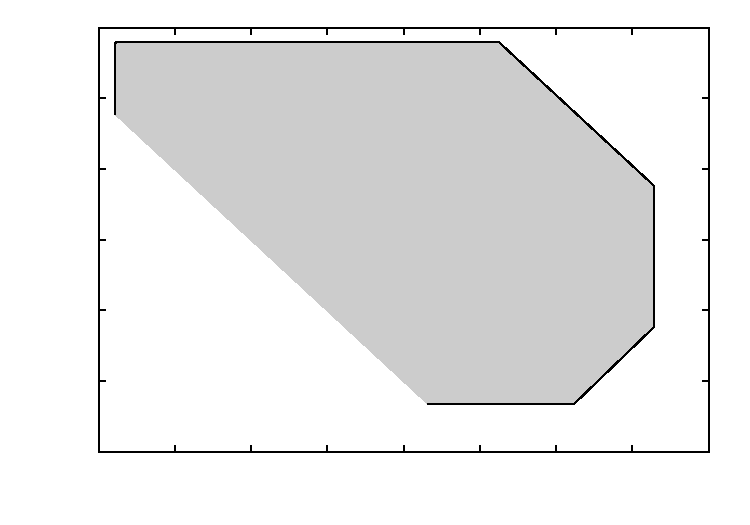
\includegraphics{esc/Xf4}}%
    \gplfronttext
  \end{picture}%
\endgroup
}
\caption{Projection of the terminal region onto the Inventory-plane
  for $\omega = 0.4$}
\label{fig:esc:Xf4}
\end{figure}


In Figure \ref{fig:esc:CL}, we plot the closed-loop response for different
values of $\omega$. We contrast the performance to a pure tracking-MPC
that tracks to the steady-state solution of the multiobjective
formulation using $\ell_T(x,u;z_p)$ as the stage cost. That is, we
compare the closed-loop from solving problem \eqref{eq:esc:PP} with the
closed-loop for $\omega = 0$ and $z_p = (x_s,u_s)$. Note that, from the
initial condition we chose $x(0) = (15,10,23,0)$, economic-MPC that
tracks to $z_s$ is only feasible for $\omega < 0.6$ (since we need
that $x(0) \geq x_s = \underbar{x}$).  

\begin{figure*}
\centering
\scriptsize
\resizebox{\textwidth}{!}{% GNUPLOT: LaTeX picture with Postscript
\begingroup
  \makeatletter
  \providecommand\color[2][]{%
    \GenericError{(gnuplot) \space\space\space\@spaces}{%
      Package color not loaded in conjunction with
      terminal option `colourtext'%
    }{See the gnuplot documentation for explanation.%
    }{Either use 'blacktext' in gnuplot or load the package
      color.sty in LaTeX.}%
    \renewcommand\color[2][]{}%
  }%
  \providecommand\includegraphics[2][]{%
    \GenericError{(gnuplot) \space\space\space\@spaces}{%
      Package graphicx or graphics not loaded%
    }{See the gnuplot documentation for explanation.%
    }{The gnuplot epslatex terminal needs graphicx.sty or graphics.sty.}%
    \renewcommand\includegraphics[2][]{}%
  }%
  \providecommand\rotatebox[2]{#2}%
  \@ifundefined{ifGPcolor}{%
    \newif\ifGPcolor
    \GPcolortrue
  }{}%
  \@ifundefined{ifGPblacktext}{%
    \newif\ifGPblacktext
    \GPblacktexttrue
  }{}%
  % define a \g@addto@macro without @ in the name:
  \let\gplgaddtomacro\g@addto@macro
  % define empty templates for all commands taking text:
  \gdef\gplbacktext{}%
  \gdef\gplfronttext{}%
  \makeatother
  \ifGPblacktext
    % no textcolor at all
    \def\colorrgb#1{}%
    \def\colorgray#1{}%
  \else
    % gray or color?
    \ifGPcolor
      \def\colorrgb#1{\color[rgb]{#1}}%
      \def\colorgray#1{\color[gray]{#1}}%
      \expandafter\def\csname LTw\endcsname{\color{white}}%
      \expandafter\def\csname LTb\endcsname{\color{black}}%
      \expandafter\def\csname LTa\endcsname{\color{black}}%
      \expandafter\def\csname LT0\endcsname{\color[rgb]{1,0,0}}%
      \expandafter\def\csname LT1\endcsname{\color[rgb]{0,1,0}}%
      \expandafter\def\csname LT2\endcsname{\color[rgb]{0,0,1}}%
      \expandafter\def\csname LT3\endcsname{\color[rgb]{1,0,1}}%
      \expandafter\def\csname LT4\endcsname{\color[rgb]{0,1,1}}%
      \expandafter\def\csname LT5\endcsname{\color[rgb]{1,1,0}}%
      \expandafter\def\csname LT6\endcsname{\color[rgb]{0,0,0}}%
      \expandafter\def\csname LT7\endcsname{\color[rgb]{1,0.3,0}}%
      \expandafter\def\csname LT8\endcsname{\color[rgb]{0.5,0.5,0.5}}%
    \else
      % gray
      \def\colorrgb#1{\color{black}}%
      \def\colorgray#1{\color[gray]{#1}}%
      \expandafter\def\csname LTw\endcsname{\color{white}}%
      \expandafter\def\csname LTb\endcsname{\color{black}}%
      \expandafter\def\csname LTa\endcsname{\color{black}}%
      \expandafter\def\csname LT0\endcsname{\color{black}}%
      \expandafter\def\csname LT1\endcsname{\color{black}}%
      \expandafter\def\csname LT2\endcsname{\color{black}}%
      \expandafter\def\csname LT3\endcsname{\color{black}}%
      \expandafter\def\csname LT4\endcsname{\color{black}}%
      \expandafter\def\csname LT5\endcsname{\color{black}}%
      \expandafter\def\csname LT6\endcsname{\color{black}}%
      \expandafter\def\csname LT7\endcsname{\color{black}}%
      \expandafter\def\csname LT8\endcsname{\color{black}}%
    \fi
  \fi
  \setlength{\unitlength}{0.0500bp}%
  \begin{picture}(7200.00,3024.00)%
    \gplgaddtomacro\gplbacktext{%
      \csname LTb\endcsname%
      \put(814,704){\makebox(0,0)[r]{\strut{} 10}}%
      \put(814,1389){\makebox(0,0)[r]{\strut{} 20}}%
      \put(814,2074){\makebox(0,0)[r]{\strut{} 30}}%
      \put(814,2759){\makebox(0,0)[r]{\strut{} 40}}%
      \put(946,484){\makebox(0,0){\strut{} 0}}%
      \put(2898,484){\makebox(0,0){\strut{} 10}}%
      \put(4851,484){\makebox(0,0){\strut{} 20}}%
      \put(6803,484){\makebox(0,0){\strut{} 30}}%
      \put(176,1731){\rotatebox{-270}{\makebox(0,0){\strut{}Inventory at Retailer}}}%
      \put(3874,154){\makebox(0,0){\strut{}Time}}%
      \put(4851,1732){\makebox(0,0)[l]{\strut{}Nominal state reset}}%
    }%
    \gplgaddtomacro\gplfronttext{%
      \csname LTb\endcsname%
      \put(4037,877){\makebox(0,0)[r]{\strut{}Actual}}%
      \csname LTb\endcsname%
      \put(5816,877){\makebox(0,0)[r]{\strut{}Nominal}}%
    }%
    \gplbacktext
    \put(0,0){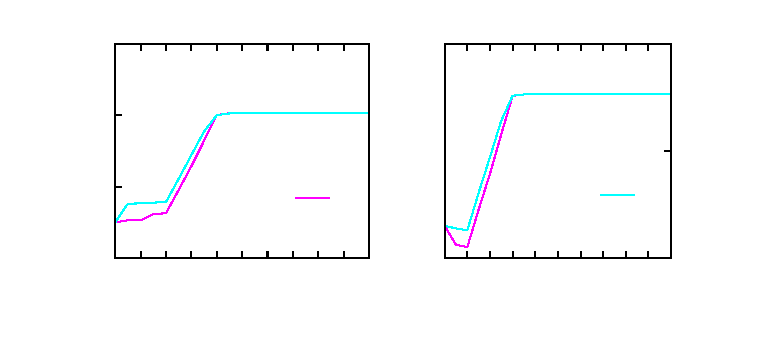
\includegraphics{CL2}}%
    \gplfronttext
  \end{picture}%
\endgroup
}
\resizebox{\textwidth}{!}{% GNUPLOT: LaTeX picture with Postscript
\begingroup
  \makeatletter
  \providecommand\color[2][]{%
    \GenericError{(gnuplot) \space\space\space\@spaces}{%
      Package color not loaded in conjunction with
      terminal option `colourtext'%
    }{See the gnuplot documentation for explanation.%
    }{Either use 'blacktext' in gnuplot or load the package
      color.sty in LaTeX.}%
    \renewcommand\color[2][]{}%
  }%
  \providecommand\includegraphics[2][]{%
    \GenericError{(gnuplot) \space\space\space\@spaces}{%
      Package graphicx or graphics not loaded%
    }{See the gnuplot documentation for explanation.%
    }{The gnuplot epslatex terminal needs graphicx.sty or graphics.sty.}%
    \renewcommand\includegraphics[2][]{}%
  }%
  \providecommand\rotatebox[2]{#2}%
  \@ifundefined{ifGPcolor}{%
    \newif\ifGPcolor
    \GPcolortrue
  }{}%
  \@ifundefined{ifGPblacktext}{%
    \newif\ifGPblacktext
    \GPblacktexttrue
  }{}%
  % define a \g@addto@macro without @ in the name:
  \let\gplgaddtomacro\g@addto@macro
  % define empty templates for all commands taking text:
  \gdef\gplbacktext{}%
  \gdef\gplfronttext{}%
  \makeatother
  \ifGPblacktext
    % no textcolor at all
    \def\colorrgb#1{}%
    \def\colorgray#1{}%
  \else
    % gray or color?
    \ifGPcolor
      \def\colorrgb#1{\color[rgb]{#1}}%
      \def\colorgray#1{\color[gray]{#1}}%
      \expandafter\def\csname LTw\endcsname{\color{white}}%
      \expandafter\def\csname LTb\endcsname{\color{black}}%
      \expandafter\def\csname LTa\endcsname{\color{black}}%
      \expandafter\def\csname LT0\endcsname{\color[rgb]{1,0,0}}%
      \expandafter\def\csname LT1\endcsname{\color[rgb]{0,1,0}}%
      \expandafter\def\csname LT2\endcsname{\color[rgb]{0,0,1}}%
      \expandafter\def\csname LT3\endcsname{\color[rgb]{1,0,1}}%
      \expandafter\def\csname LT4\endcsname{\color[rgb]{0,1,1}}%
      \expandafter\def\csname LT5\endcsname{\color[rgb]{1,1,0}}%
      \expandafter\def\csname LT6\endcsname{\color[rgb]{0,0,0}}%
      \expandafter\def\csname LT7\endcsname{\color[rgb]{1,0.3,0}}%
      \expandafter\def\csname LT8\endcsname{\color[rgb]{0.5,0.5,0.5}}%
    \else
      % gray
      \def\colorrgb#1{\color{black}}%
      \def\colorgray#1{\color[gray]{#1}}%
      \expandafter\def\csname LTw\endcsname{\color{white}}%
      \expandafter\def\csname LTb\endcsname{\color{black}}%
      \expandafter\def\csname LTa\endcsname{\color{black}}%
      \expandafter\def\csname LT0\endcsname{\color{black}}%
      \expandafter\def\csname LT1\endcsname{\color{black}}%
      \expandafter\def\csname LT2\endcsname{\color{black}}%
      \expandafter\def\csname LT3\endcsname{\color{black}}%
      \expandafter\def\csname LT4\endcsname{\color{black}}%
      \expandafter\def\csname LT5\endcsname{\color{black}}%
      \expandafter\def\csname LT6\endcsname{\color{black}}%
      \expandafter\def\csname LT7\endcsname{\color{black}}%
      \expandafter\def\csname LT8\endcsname{\color{black}}%
    \fi
  \fi
  \setlength{\unitlength}{0.0500bp}%
  \begin{picture}(7200.00,3024.00)%
    \gplgaddtomacro\gplbacktext{%
      \csname LTb\endcsname%
      \put(814,704){\makebox(0,0)[r]{\strut{} 0}}%
      \put(814,1389){\makebox(0,0)[r]{\strut{} 10}}%
      \put(814,2074){\makebox(0,0)[r]{\strut{} 20}}%
      \put(814,2759){\makebox(0,0)[r]{\strut{} 30}}%
      \put(946,484){\makebox(0,0){\strut{} 0}}%
      \put(1555,484){\makebox(0,0){\strut{} 5}}%
      \put(2165,484){\makebox(0,0){\strut{} 10}}%
      \put(2774,484){\makebox(0,0){\strut{} 15}}%
      \put(3383,484){\makebox(0,0){\strut{} 20}}%
      \put(176,1731){\rotatebox{-270}{\makebox(0,0){\strut{}Retailer-Inventory}}}%
      \put(2164,154){\makebox(0,0){\strut{}Time}}%
    }%
    \gplgaddtomacro\gplfronttext{%
      \csname LTb\endcsname%
      \put(2660,2586){\makebox(0,0)[r]{\strut{}Multiobjective}}%
      \csname LTb\endcsname%
      \put(2660,2366){\makebox(0,0)[r]{\strut{}Tracking}}%
    }%
    \gplgaddtomacro\gplbacktext{%
      \csname LTb\endcsname%
      \put(4109,484){\makebox(0,0){\strut{} 0}}%
      \put(4652,484){\makebox(0,0){\strut{} 5}}%
      \put(5196,484){\makebox(0,0){\strut{} 10}}%
      \put(5739,484){\makebox(0,0){\strut{} 15}}%
      \put(6282,484){\makebox(0,0){\strut{} 20}}%
      \put(6414,704){\makebox(0,0)[l]{\strut{} 10}}%
      \put(6414,1732){\makebox(0,0)[l]{\strut{} 20}}%
      \put(6414,2759){\makebox(0,0)[l]{\strut{} 30}}%
      \put(7051,1731){\rotatebox{-270}{\makebox(0,0){\strut{}Manufacturer-Inventory}}}%
      \put(5195,154){\makebox(0,0){\strut{}Time}}%
    }%
    \gplgaddtomacro\gplfronttext{%
    }%
    \gplbacktext
    \put(0,0){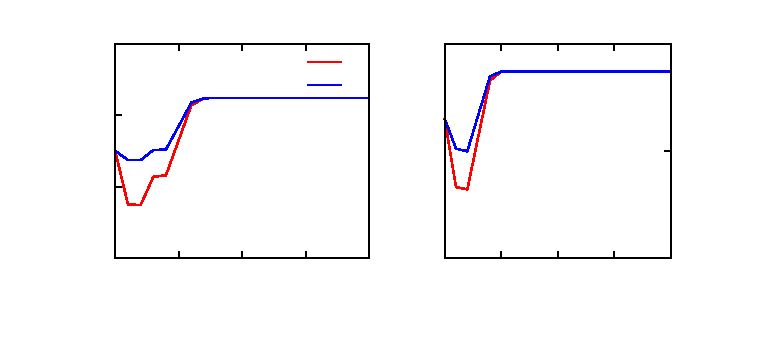
\includegraphics{CL4}}%
    \gplfronttext
  \end{picture}%
\endgroup
}
\resizebox{\textwidth}{!}{% GNUPLOT: LaTeX picture with Postscript
\begingroup
  \makeatletter
  \providecommand\color[2][]{%
    \GenericError{(gnuplot) \space\space\space\@spaces}{%
      Package color not loaded in conjunction with
      terminal option `colourtext'%
    }{See the gnuplot documentation for explanation.%
    }{Either use 'blacktext' in gnuplot or load the package
      color.sty in LaTeX.}%
    \renewcommand\color[2][]{}%
  }%
  \providecommand\includegraphics[2][]{%
    \GenericError{(gnuplot) \space\space\space\@spaces}{%
      Package graphicx or graphics not loaded%
    }{See the gnuplot documentation for explanation.%
    }{The gnuplot epslatex terminal needs graphicx.sty or graphics.sty.}%
    \renewcommand\includegraphics[2][]{}%
  }%
  \providecommand\rotatebox[2]{#2}%
  \@ifundefined{ifGPcolor}{%
    \newif\ifGPcolor
    \GPcolorfalse
  }{}%
  \@ifundefined{ifGPblacktext}{%
    \newif\ifGPblacktext
    \GPblacktexttrue
  }{}%
  % define a \g@addto@macro without @ in the name:
  \let\gplgaddtomacro\g@addto@macro
  % define empty templates for all commands taking text:
  \gdef\gplbacktext{}%
  \gdef\gplfronttext{}%
  \makeatother
  \ifGPblacktext
    % no textcolor at all
    \def\colorrgb#1{}%
    \def\colorgray#1{}%
  \else
    % gray or color?
    \ifGPcolor
      \def\colorrgb#1{\color[rgb]{#1}}%
      \def\colorgray#1{\color[gray]{#1}}%
      \expandafter\def\csname LTw\endcsname{\color{white}}%
      \expandafter\def\csname LTb\endcsname{\color{black}}%
      \expandafter\def\csname LTa\endcsname{\color{black}}%
      \expandafter\def\csname LT0\endcsname{\color[rgb]{1,0,0}}%
      \expandafter\def\csname LT1\endcsname{\color[rgb]{0,1,0}}%
      \expandafter\def\csname LT2\endcsname{\color[rgb]{0,0,1}}%
      \expandafter\def\csname LT3\endcsname{\color[rgb]{1,0,1}}%
      \expandafter\def\csname LT4\endcsname{\color[rgb]{0,1,1}}%
      \expandafter\def\csname LT5\endcsname{\color[rgb]{1,1,0}}%
      \expandafter\def\csname LT6\endcsname{\color[rgb]{0,0,0}}%
      \expandafter\def\csname LT7\endcsname{\color[rgb]{1,0.3,0}}%
      \expandafter\def\csname LT8\endcsname{\color[rgb]{0.5,0.5,0.5}}%
    \else
      % gray
      \def\colorrgb#1{\color{black}}%
      \def\colorgray#1{\color[gray]{#1}}%
      \expandafter\def\csname LTw\endcsname{\color{white}}%
      \expandafter\def\csname LTb\endcsname{\color{black}}%
      \expandafter\def\csname LTa\endcsname{\color{black}}%
      \expandafter\def\csname LT0\endcsname{\color{black}}%
      \expandafter\def\csname LT1\endcsname{\color{black}}%
      \expandafter\def\csname LT2\endcsname{\color{black}}%
      \expandafter\def\csname LT3\endcsname{\color{black}}%
      \expandafter\def\csname LT4\endcsname{\color{black}}%
      \expandafter\def\csname LT5\endcsname{\color{black}}%
      \expandafter\def\csname LT6\endcsname{\color{black}}%
      \expandafter\def\csname LT7\endcsname{\color{black}}%
      \expandafter\def\csname LT8\endcsname{\color{black}}%
    \fi
  \fi
  \setlength{\unitlength}{0.0500bp}%
  \begin{picture}(7200.00,3024.00)%
    \gplgaddtomacro\gplbacktext{%
      \csname LTb\endcsname%
      \put(814,704){\makebox(0,0)[r]{\strut{} 0}}%
      \put(814,1732){\makebox(0,0)[r]{\strut{} 10}}%
      \put(814,2759){\makebox(0,0)[r]{\strut{} 20}}%
      \put(946,484){\makebox(0,0){\strut{} 0}}%
      \put(1190,484){\makebox(0,0){\strut{} 2}}%
      \put(1433,484){\makebox(0,0){\strut{} 4}}%
      \put(1677,484){\makebox(0,0){\strut{} 6}}%
      \put(1921,484){\makebox(0,0){\strut{} 8}}%
      \put(2165,484){\makebox(0,0){\strut{} 10}}%
      \put(2408,484){\makebox(0,0){\strut{} 12}}%
      \put(2652,484){\makebox(0,0){\strut{} 14}}%
      \put(2896,484){\makebox(0,0){\strut{} 16}}%
      \put(3139,484){\makebox(0,0){\strut{} 18}}%
      \put(3383,484){\makebox(0,0){\strut{} 20}}%
      \put(176,1731){\rotatebox{-270}{\makebox(0,0){\strut{}Inventory}}}%
      \put(2164,154){\makebox(0,0){\strut{}Time}}%
      \put(1921,2245){\makebox(0,0)[l]{\strut{}$\omega = 0.8$}}%
    }%
    \gplgaddtomacro\gplfronttext{%
    }%
    \gplgaddtomacro\gplbacktext{%
      \csname LTb\endcsname%
      \put(4109,484){\makebox(0,0){\strut{} 0}}%
      \put(4326,484){\makebox(0,0){\strut{} 2}}%
      \put(4544,484){\makebox(0,0){\strut{} 4}}%
      \put(4761,484){\makebox(0,0){\strut{} 6}}%
      \put(4978,484){\makebox(0,0){\strut{} 8}}%
      \put(5196,484){\makebox(0,0){\strut{} 10}}%
      \put(5413,484){\makebox(0,0){\strut{} 12}}%
      \put(5630,484){\makebox(0,0){\strut{} 14}}%
      \put(5847,484){\makebox(0,0){\strut{} 16}}%
      \put(6065,484){\makebox(0,0){\strut{} 18}}%
      \put(6282,484){\makebox(0,0){\strut{} 20}}%
      \put(6414,704){\makebox(0,0)[l]{\strut{} 0}}%
      \put(6414,1389){\makebox(0,0)[l]{\strut{} 10}}%
      \put(6414,2074){\makebox(0,0)[l]{\strut{} 20}}%
      \put(6414,2759){\makebox(0,0)[l]{\strut{} 30}}%
      \put(7051,1731){\rotatebox{-270}{\makebox(0,0){\strut{}Inventory}}}%
      \put(5195,154){\makebox(0,0){\strut{}Time}}%
    }%
    \gplgaddtomacro\gplfronttext{%
    }%
    \gplbacktext
    \put(0,0){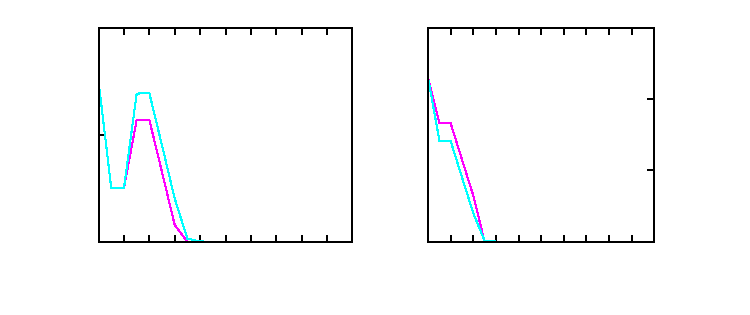
\includegraphics{CL8}}%
    \gplfronttext
  \end{picture}%
\endgroup
}
\caption{Closed-loop response for $\omega = 0.2$ (top), $\omega = 0.4$
(middle) and $\omega = 0.8$ (bottom)}
\label{fig:esc:CL}
\end{figure*}

In Table \ref{tab:esc:CL}, we compare the economic cost incurred in using
the three controllers: (i) Multiobjective MPC $\ell(x,u;z_p)$, (ii)
Economic MPC $\ell_E(x,u)$ and (iii) Tracking MPC to the steady-state
of the multiobjective MPC $\ell_T(x,u,z_s)$. 

\begin{table}[h]
\caption{Economic cost of implementing MPC}
\label{tab:esc:CL}
\begin{center}
\begin{tabular}{cccc}\toprule
$\omega$ & Multiobjective$ _{ \times 10^{4}}$ & Tracking$ _{ \times 10^{4}}$ & Economic$ _{ \times 10^{4}}$ \\
%& \hfill$ _{ \times 10^{4}}$ & \hfill$_{\times 10^{4}}$ &\hfill
%$_{\times 10^{4}}$ \\
\midrule
0 & 4.4342 & 4.4342 & infeasible \\
0.2 & 4.0246 & 4.0645 & infeasible \\
0.4 & 3.5617 & 3.6252 & infeasible \\
%0.6 & 2.7343 & 2.7380 & 2.7380 (stabilizes origin) \\
0.8 & 2.2670 & 2.2670 & 2.2670 \\
1.0 & 2.2670 & 2.2670 & 2.2670 \\
\bottomrule
\end{tabular}
\end{center}
\end{table}

We observe that as $\omega$ increases, that is, as the economic costs
are given more weight, the steady-state approaches the constraint
boundary. In such situations, the optimal input profile is dominated
by feasibility and as such all the three stage costs incur the same
economic cost in the closed loop \footnote{We optimize the open-loop
  cost. The numbers in Table \ref{tab:esc:CL} are just the economic
  cost of implementing the optimal input}. However, for intermediate values of
$\omega$, that is, when the practitioner has comparable weighting to
both tracking the safety stock and minimizing costs,
multiobjective-MPC gives the best performance. While in the tracking
MPC, we can design the system go to the same steady-state as multiobjective, the absence of
economic knowledge in the tracking stage cost means that some
economically more attractive transients are not considered by the
online optimizer. While designing a controller that minimizes only the
costs seems very attractive, the drawback is that for supply chains, such economic MPC can only stabilize steady states
that lie on the one of the vertices of the constraint set. Therefore,
we cannot use pure economic MPC to track the inventories to a target
value. 

\section{Multi-product, multi-echelon supply chain example}
\label{sec:esc:multi}
In this section, we follow the design procedure described in the
previous section to implement model predictive control for a
multi-product, multi-echelon supply chain. The supply chain that is
studied is shown in Figure \ref{fig:esc:lssc}. It consists of a
manufacturing facility $M1$ that supplies two products $A,B$ to two
distribution centers $D1,D2$ and a retailer $R5$. Distribution center
$D1$ supplies the products to retailers $R1,R2$ while distribution
center $D2$ supplies to $R3$ and $R4$. 

\begin{figure}
\centering
\scriptsize
\resizebox{0.5\textwidth}{!}{\begin{picture}(0,0)%
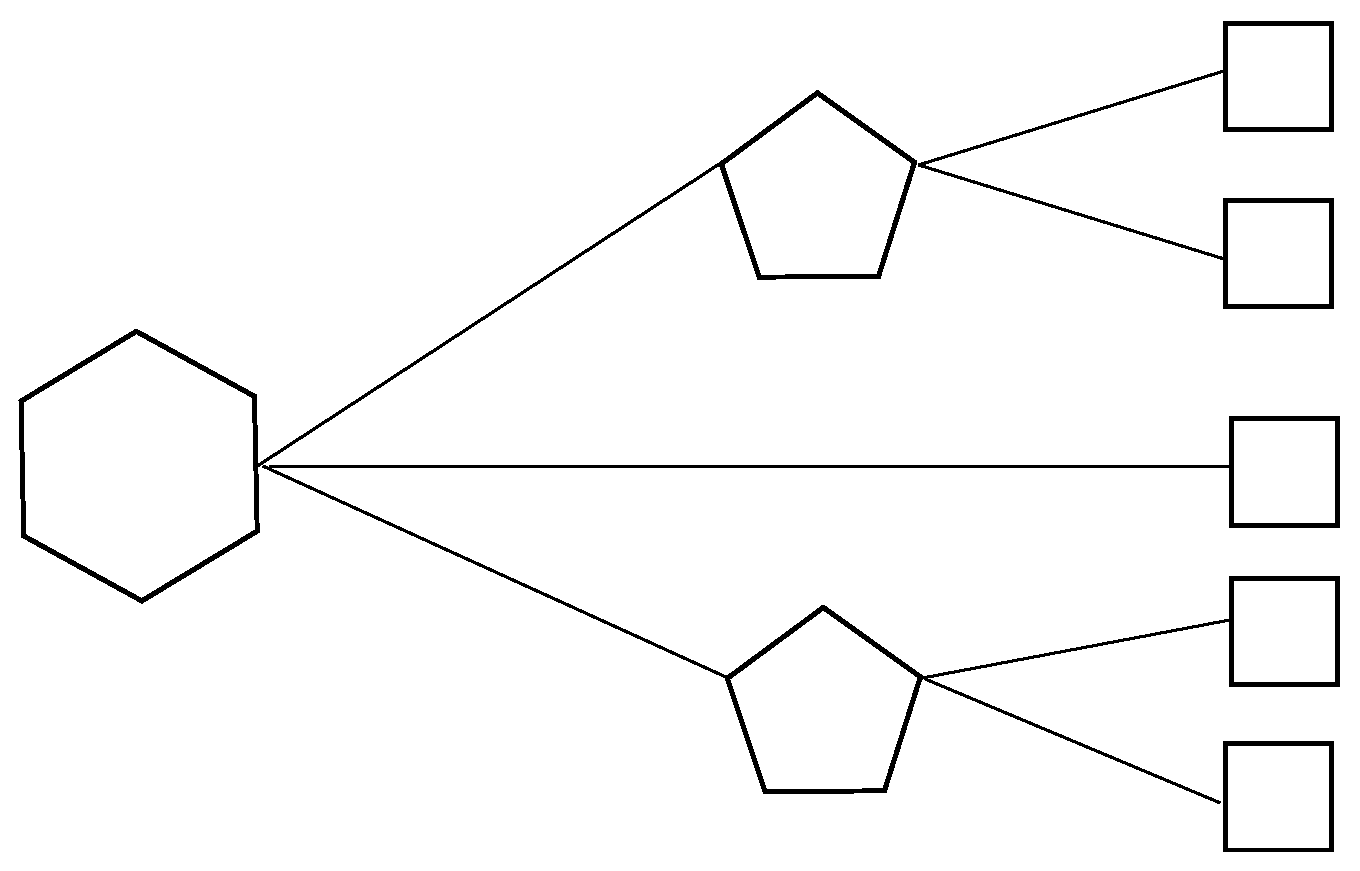
\includegraphics{esc/lssc}%
\end{picture}%
\setlength{\unitlength}{4144sp}%
%
\begingroup\makeatletter\ifx\SetFigFont\undefined%
\gdef\SetFigFont#1#2#3#4#5{%
  \reset@font\fontsize{#1}{#2pt}%
  \fontfamily{#3}\fontseries{#4}\fontshape{#5}%
  \selectfont}%
\fi\endgroup%
\begin{picture}(10101,6366)(1363,-5719)
\put(10801,164){\makebox(0,0)[lb]{\smash{{\SetFigFont{17}{20.4}{\familydefault}{\mddefault}{\updefault}{\color[rgb]{0,0,0}$R1$}%
}}}}
\put(2071,-2851){\makebox(0,0)[lb]{\smash{{\SetFigFont{17}{20.4}{\familydefault}{\mddefault}{\updefault}{\color[rgb]{0,0,0}$M1$}%
}}}}
\put(7246,-736){\makebox(0,0)[lb]{\smash{{\SetFigFont{17}{20.4}{\familydefault}{\mddefault}{\updefault}{\color[rgb]{0,0,0}$D1$}%
}}}}
\put(7291,-4741){\makebox(0,0)[lb]{\smash{{\SetFigFont{17}{20.4}{\familydefault}{\mddefault}{\updefault}{\color[rgb]{0,0,0}$D2$}%
}}}}
\put(10801,-5371){\makebox(0,0)[lb]{\smash{{\SetFigFont{17}{20.4}{\familydefault}{\mddefault}{\updefault}{\color[rgb]{0,0,0}$R4$}%
}}}}
\put(10846,-4111){\makebox(0,0)[lb]{\smash{{\SetFigFont{17}{20.4}{\familydefault}{\mddefault}{\updefault}{\color[rgb]{0,0,0}$R3$}%
}}}}
\put(10891,-2896){\makebox(0,0)[lb]{\smash{{\SetFigFont{17}{20.4}{\familydefault}{\mddefault}{\updefault}{\color[rgb]{0,0,0}$R5$}%
}}}}
\put(10801,-1231){\makebox(0,0)[lb]{\smash{{\SetFigFont{17}{20.4}{\familydefault}{\mddefault}{\updefault}{\color[rgb]{0,0,0}$R2$}%
}}}}
\end{picture}%
}
\caption{Multi-product, Multi-echelon supply chain studied}
\label{fig:esc:lssc}
\end{figure}

We list the production lead-times at the manufacturing facility in
Table \ref{tab:esc:prodlead}. We assume that the manufacturing facility is
able to produce both products simultaneously, with the only limitation
being the combined storage of these products in the manufacturing
node's storage facility (see Table \ref{tab:esc:constraints}).In Table \ref{tab:esc:translead}, we list the transportation times between
each node.
 
\begin{table}
\caption{Production lead-times}
\label{tab:esc:prodlead}
\begin{center}
\begin{tabular}{cc}\toprule
Product& Lead-time \\
\midrule
$A$ & 2\\
$B$ & 3\\
\bottomrule
\end{tabular}
\end{center}
\caption{Transportation lead-times}
\label{tab:esc:translead}
\begin{center}
\begin{tabular}{cccccccc}\toprule
& $D1$ & $D2$  & $R1$ & $R2$ & $R3$ & $R4$ & $R5$ \\
\midrule
$M1$ &2&1& & & & &4\\
$D1$ & & &1&1& & & \\
$D2$ & & & & &2&1& \\
\bottomrule
\end{tabular}
\end{center}
\caption{Nominal demand}
\begin{center}
\begin{tabular}{cccccc}\toprule
\label{tab:esc:nomdem}
 &$R1$&$R2$&$R3$&$R4$&$R5$\\
\midrule
$A$&3.0&4.5&5.0&2.0&4.0\\
$B$&4.2&3.1&1.4&2.5&4.2\\
\bottomrule
\end{tabular}
\end{center}
\caption{Variance of  demand}
\begin{center}
\begin{tabular}{cccccc}\toprule
\label{tab:esc:vardem}
 &$R1$&$R2$&$R3$&$R4$&$R5$\\
\midrule
$A$&1.1&1.3&1.1&1.2&1.4\\
$B$&1.3&1.4&1.1&1.1&1.4\\
\bottomrule
\end{tabular}
\end{center}
\end{table}




The retailers respond to customer demands which is assumed to arrive
at each period following a normal distribution around a nominal
demand. The nominal demand for each retailer node is listed in Table
\ref{tab:esc:nomdem} while the variance of the demand signal in each retailer node for
both products are listed in Table \ref{tab:esc:vardem}


For each node, we choose the target inventory to be the amount of
product to be carried so that demands can be met for as long as the
longest delay in the supply chain. The longest delay in the supply
chain is 4 (the transportation time between $M1$ and $R5$). Hence, for
the retailers, we choose the target inventory to be four times the
nominal demand. For the distributors, the target inventory is four
times the nominal demand at the distributor. The nominal demand at the
distributor is the sum of the demands at the retailers that is served
by the distributor. 

\begin{table}
\caption{Target inventories}
\label{tab:esc:targinv}
\begin{center}
\begin{tabular}{ccccccccc}\toprule
& $M1$ & $D1$ & $D2$  & $R1$ & $R2$ & $R3$ & $R4$ & $R5$ \\
\midrule
$A$&70&30  &24   &12  &18  &20 &8 &16\\
$B$&61&29.2&15.6 &16.8&12.4&5.6&10&16.8 \\
\bottomrule
\end{tabular}
\end{center}
\caption{Capacity constraints}
\label{tab:esc:constraints}
\begin{center}
\begin{tabular}{ccccccccc}\toprule
& $M1$ & $D1$ & $D2$  & $R1$ & $R2$ & $R3$ & $R4$ & $R5$ \\
\midrule
$\Inv_A+\Inv_B$&140&80  &50   &40  &40  &30 &25 &45\\
\bottomrule
\end{tabular}
\end{center}
\caption{State economic costs}
\label{tab:esc:state_economic}
\begin{center}
\begin{tabular}{ccccccccc}\toprule
& $M1$ & $D1$ & $D2$  & $R1$ & $R2$ & $R3$ & $R4$ & $R5$ \\
\midrule
Inventory holding&1&1  &1   &1  &1  &1 &1 &1\\
Back-order&10&10&10 &10&10&10&10&10 \\
\bottomrule
\end{tabular}
\end{center}
\caption{Input costs}
\label{tab:esc:input_economic}
\begin{center}
\begin{tabular}{cccccccc}\toprule
& $D1$ & $D2$  & $R1$ & $R2$ & $R3$ & $R4$ & $R5$ \\
\midrule
$M1$ &(4,2)&(1,2)& & & & &(5,4)\\
$D1$ & & &(1,1)&(1,1)& & & \\
$D2$ & & & & &(2,2)&(1.5,1.5)& \\
\bottomrule
\end{tabular}
\end{center}
\end{table}

The target back-orders in each node is $0$.

As mentioned earlier, each node has a combined inventory storage
capacity. This capacity is listed in Table \ref{tab:esc:constraints}. The
maximum storage is chosen to be greater than the target inventories.


The economic objective is the sum of the (i) inventory holding costs
(ii) back-order costs and (iii) shipping and ordering costs. The
coefficients for these costs are listed in the following tables.

In table \ref{tab:esc:input_economic}, each entry corresponds to the
shipping cost of product $A$ and product $B$ respectively. In
addition, the cost coefficient of shipping products to the
customers from the retailers is $1$.

The ordering costs coefficients are all chosen to be $1$, except for
ordering between the $R5$ and $M1$ for which the cost-coefficient is
chosen to be $0.5$. 

The production costs for product $A$ is 10 per unit while that for $B$
is 4 per unit.


The tracking objective is a weighted sum of the squares of the
deviation of the inventories(and backorders) from their targets. These
weights are chosen as $1$ for inventory deviation (that is, we
penalize $(\Inv-\Inv_t)^2$), 10 for backorder deviation
($10(\BO-\BO_t)^2$). The inputs are penalized from their targets with
a weight of $0.1$ (the input targets are chosen to be the steady-state
values as described below).


With the aforementioned details about the supply chain, the supply
chain model can be written in the state space format \eqref{eq:esc:model} and the stage
costs $\ell_E(\cdot,\cdot)$, \eqref{eq:esc:ellE} and
$\ell_T(\cdot,\cdot)$, \eqref{eq:esc:ellT} is defined.  Choosing an
economic objective weight of $0.4$, we can solve for the steady-state
problem \eqref{eq:esc:SSMulti} to obtain the steady state. As discussed in
the previous section, the multiobjective steady state lies between a
pure tracking ($\omega = 0$) and a pure economic $(\omega=1)$ steady
state. We re-iterate that the input steady-state remains the same
irrespective of the objective function, because of the steady-state
constraint that fixes all the flows in the supply chain in accordance
with the nominal demand. In Table \ref{tab:esc:steady}, we list the
inventory steady-states (for product-A) for the pure economic, tracking and the
multiobjective cost functions.


\begin{table}[h]
\caption{Steady state  inventories for product $A$}
\label{tab:esc:steady}
\begin{center}
\begin{tabular}{ccccccccc}\toprule
& $M1$ & $D1$ & $D2$  & $R1$ & $R2$ & $R3$ & $R4$ & $R5$ \\
\midrule
Tracking                      &70   &30   &24   &12&18  &20  &8&16 \\
Economic                      &0    &0    &0    &0 &0   &0   &0&0   \\
Multiobjective($\omega = 0.4$)&57.93&17.93&11.93&0 &5.93&7.93&0&3.93\\
\bottomrule
\end{tabular}
\end{center}
\end{table}

\paragraph{$(\sigma,\Sigma) $ Policy.} We compare the closed-loop operation of
the centralized multi-objective supply chain with that of the
closed-loop dynamics due to a $(\sigma,\Sigma) $ policy. In the $(\sigma,\Sigma) $
policy, the nodes orders according to the
following shipping and ordering policies. We denote the shipments coming from the upstream
node as $S^{u}$, while the orders coming from downstream (demand for
the retailer as $O^{d}$.
\begin{equation}
S(t) = \begin{cases} O^{d}(t)+\BO(t) \quad \text{if~}
  \Inv(t)+S^{u}(t)-(O^{d}(t)+\BO(t)) \geq 0 \\
  \Inv(t)+S^{u}(t)\quad \text{otherwise}
  \end{cases}
\end{equation}

Having determined the shipment at time $k$, the node then places
orders according to the inventory and backorder levels that the
shipments will lead to at the next time as:
\begin{equation}
O(t) = \begin{cases} \Sigma - (\Inv(t+1)-\BO(t+1)) \quad
  \text{if~} (\Inv(t+1)-\BO(t+1)) \leq \sigma\\
0 \quad \text{otherwise~}
\end{cases}
\end{equation}

The $(\sigma,\Sigma)$ policy is a decentralized linear feedback policy. The retailer
observes the demands, makes its ordering decisions which is then used
by the distributor and so on. 

\subsection{Results}
The supply chain described in the previous section was simulated for
50 days using a stochastic demand signal. The terminal
condition used was that the system should be at the steady-state
at the end of the prediction horizon,
which was chosen as 15 days. Furthermore, we assumed that the MPC
controller had perfect demand information for three days. For the
remainder of the prediction horizon, we used the nominal demands as
the demand forecast. For the $(\sigma,\Sigma)$ policy, we chose
$\sigma = 0.7\Sigma$ and $\Sigma$ as the steady state inventory. 

The initial inventories of the nodes were chosen as follows:
\begin{table}[h]
\caption{Initial inventories}
\label{tab:esc:initial}
\begin{center}
\begin{tabular}{ccccccccc}\toprule
& $M1$ & $D1$ & $D2$  & $R1$ & $R2$ & $R3$ & $R4$ & $R5$ \\
\midrule
$A$                      &63   &14   &24   &0 &2.1  &3.1  &3.1&0 \\
$B$                      &40   &12   &7    &0 &1.2  &1.2  &0  &5.2   \\
\bottomrule
\end{tabular}
\end{center}
\end{table}
All the backorders were $0$ and the inputs were at their steady-state
at the begining of the simulation.

In Figure \ref{fig:esc:bullwhip}, we report the ordering-profile in the supply
chain, and compare the variance of the demands observed with the
variance of the orders placed as we move upstream in the node. The
variance in orders placed as we move upstream is an measure of the
bullwhip effect. We see that the the MPC policy has less variance in
ordering profile as we move upstream in the supply chain. This lower
variance is because the MPC controller is a centralized controller that not only
considers all the nodes together, but also makes predictions for two
weeks into the future. Therefore, at certain nodes, the MPC controller is able to take
advantage of higher inventory levels than the steady state inventory
to place fewer orders in total. The $(\sigma,\Sigma)$ policy shows the
classical bullwhip effect of the variance of the orders increasing as
we move upstream. In Figure \ref{fig:esc:Order}, we plot the orders placed by the MPC
controller and the $(\sigma,\Sigma)$ policy controller in response to
demands of product $A$ at Retailer $R3$.


\begin{figure}
\centering
\scriptsize
\resizebox{1\textwidth}{!}{% GNUPLOT: LaTeX picture with Postscript
\begingroup
  \makeatletter
  \providecommand\color[2][]{%
    \GenericError{(gnuplot) \space\space\space\@spaces}{%
      Package color not loaded in conjunction with
      terminal option `colourtext'%
    }{See the gnuplot documentation for explanation.%
    }{Either use 'blacktext' in gnuplot or load the package
      color.sty in LaTeX.}%
    \renewcommand\color[2][]{}%
  }%
  \providecommand\includegraphics[2][]{%
    \GenericError{(gnuplot) \space\space\space\@spaces}{%
      Package graphicx or graphics not loaded%
    }{See the gnuplot documentation for explanation.%
    }{The gnuplot epslatex terminal needs graphicx.sty or graphics.sty.}%
    \renewcommand\includegraphics[2][]{}%
  }%
  \providecommand\rotatebox[2]{#2}%
  \@ifundefined{ifGPcolor}{%
    \newif\ifGPcolor
    \GPcolortrue
  }{}%
  \@ifundefined{ifGPblacktext}{%
    \newif\ifGPblacktext
    \GPblacktexttrue
  }{}%
  % define a \g@addto@macro without @ in the name:
  \let\gplgaddtomacro\g@addto@macro
  % define empty templates for all commands taking text:
  \gdef\gplbacktext{}%
  \gdef\gplfronttext{}%
  \makeatother
  \ifGPblacktext
    % no textcolor at all
    \def\colorrgb#1{}%
    \def\colorgray#1{}%
  \else
    % gray or color?
    \ifGPcolor
      \def\colorrgb#1{\color[rgb]{#1}}%
      \def\colorgray#1{\color[gray]{#1}}%
      \expandafter\def\csname LTw\endcsname{\color{white}}%
      \expandafter\def\csname LTb\endcsname{\color{black}}%
      \expandafter\def\csname LTa\endcsname{\color{black}}%
      \expandafter\def\csname LT0\endcsname{\color[rgb]{1,0,0}}%
      \expandafter\def\csname LT1\endcsname{\color[rgb]{0,1,0}}%
      \expandafter\def\csname LT2\endcsname{\color[rgb]{0,0,1}}%
      \expandafter\def\csname LT3\endcsname{\color[rgb]{1,0,1}}%
      \expandafter\def\csname LT4\endcsname{\color[rgb]{0,1,1}}%
      \expandafter\def\csname LT5\endcsname{\color[rgb]{1,1,0}}%
      \expandafter\def\csname LT6\endcsname{\color[rgb]{0,0,0}}%
      \expandafter\def\csname LT7\endcsname{\color[rgb]{1,0.3,0}}%
      \expandafter\def\csname LT8\endcsname{\color[rgb]{0.5,0.5,0.5}}%
    \else
      % gray
      \def\colorrgb#1{\color{black}}%
      \def\colorgray#1{\color[gray]{#1}}%
      \expandafter\def\csname LTw\endcsname{\color{white}}%
      \expandafter\def\csname LTb\endcsname{\color{black}}%
      \expandafter\def\csname LTa\endcsname{\color{black}}%
      \expandafter\def\csname LT0\endcsname{\color{black}}%
      \expandafter\def\csname LT1\endcsname{\color{black}}%
      \expandafter\def\csname LT2\endcsname{\color{black}}%
      \expandafter\def\csname LT3\endcsname{\color{black}}%
      \expandafter\def\csname LT4\endcsname{\color{black}}%
      \expandafter\def\csname LT5\endcsname{\color{black}}%
      \expandafter\def\csname LT6\endcsname{\color{black}}%
      \expandafter\def\csname LT7\endcsname{\color{black}}%
      \expandafter\def\csname LT8\endcsname{\color{black}}%
    \fi
  \fi
  \setlength{\unitlength}{0.0500bp}%
  \begin{picture}(7200.00,3024.00)%
    \gplgaddtomacro\gplbacktext{%
      \csname LTb\endcsname%
      \put(682,846){\makebox(0,0)[r]{\strut{} 0}}%
      \put(682,1119){\makebox(0,0)[r]{\strut{} 1}}%
      \put(682,1393){\makebox(0,0)[r]{\strut{} 2}}%
      \put(682,1666){\makebox(0,0)[r]{\strut{} 3}}%
      \put(682,1939){\makebox(0,0)[r]{\strut{} 4}}%
      \put(682,2212){\makebox(0,0)[r]{\strut{} 5}}%
      \put(682,2486){\makebox(0,0)[r]{\strut{} 6}}%
      \put(682,2759){\makebox(0,0)[r]{\strut{} 7}}%
      \put(2012,714){\rotatebox{-45}{\makebox(0,0)[l]{\strut{}R1}}}%
      \put(3210,714){\rotatebox{-45}{\makebox(0,0)[l]{\strut{}R5}}}%
      \put(4407,714){\rotatebox{-45}{\makebox(0,0)[l]{\strut{}D1}}}%
      \put(5605,714){\rotatebox{-45}{\makebox(0,0)[l]{\strut{}D2}}}%
      \put(176,1802){\rotatebox{-270}{\makebox(0,0){\strut{}Standard deviation of Orders}}}%
    }%
    \gplgaddtomacro\gplfronttext{%
      \csname LTb\endcsname%
      \put(1998,173){\makebox(0,0)[r]{\strut{}Incoming}}%
      \csname LTb\endcsname%
      \put(3909,173){\makebox(0,0)[r]{\strut{}MPC}}%
      \csname LTb\endcsname%
      \put(5820,173){\makebox(0,0)[r]{\strut{}$(\sigma,\Sigma)$}}%
    }%
    \gplbacktext
    \put(0,0){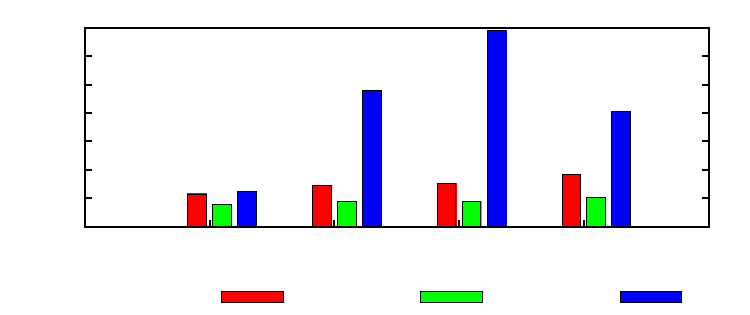
\includegraphics{esc/bullwhip}}%
    \gplfronttext
  \end{picture}%
\endgroup
}
\caption{Bullwhip effect}
\label{fig:esc:bullwhip}
\centering
\scriptsize
\resizebox{1\textwidth}{!}{% GNUPLOT: LaTeX picture with Postscript
\begingroup
  \makeatletter
  \providecommand\color[2][]{%
    \GenericError{(gnuplot) \space\space\space\@spaces}{%
      Package color not loaded in conjunction with
      terminal option `colourtext'%
    }{See the gnuplot documentation for explanation.%
    }{Either use 'blacktext' in gnuplot or load the package
      color.sty in LaTeX.}%
    \renewcommand\color[2][]{}%
  }%
  \providecommand\includegraphics[2][]{%
    \GenericError{(gnuplot) \space\space\space\@spaces}{%
      Package graphicx or graphics not loaded%
    }{See the gnuplot documentation for explanation.%
    }{The gnuplot epslatex terminal needs graphicx.sty or graphics.sty.}%
    \renewcommand\includegraphics[2][]{}%
  }%
  \providecommand\rotatebox[2]{#2}%
  \@ifundefined{ifGPcolor}{%
    \newif\ifGPcolor
    \GPcolortrue
  }{}%
  \@ifundefined{ifGPblacktext}{%
    \newif\ifGPblacktext
    \GPblacktexttrue
  }{}%
  % define a \g@addto@macro without @ in the name:
  \let\gplgaddtomacro\g@addto@macro
  % define empty templates for all commands taking text:
  \gdef\gplbacktext{}%
  \gdef\gplfronttext{}%
  \makeatother
  \ifGPblacktext
    % no textcolor at all
    \def\colorrgb#1{}%
    \def\colorgray#1{}%
  \else
    % gray or color?
    \ifGPcolor
      \def\colorrgb#1{\color[rgb]{#1}}%
      \def\colorgray#1{\color[gray]{#1}}%
      \expandafter\def\csname LTw\endcsname{\color{white}}%
      \expandafter\def\csname LTb\endcsname{\color{black}}%
      \expandafter\def\csname LTa\endcsname{\color{black}}%
      \expandafter\def\csname LT0\endcsname{\color[rgb]{1,0,0}}%
      \expandafter\def\csname LT1\endcsname{\color[rgb]{0,1,0}}%
      \expandafter\def\csname LT2\endcsname{\color[rgb]{0,0,1}}%
      \expandafter\def\csname LT3\endcsname{\color[rgb]{1,0,1}}%
      \expandafter\def\csname LT4\endcsname{\color[rgb]{0,1,1}}%
      \expandafter\def\csname LT5\endcsname{\color[rgb]{1,1,0}}%
      \expandafter\def\csname LT6\endcsname{\color[rgb]{0,0,0}}%
      \expandafter\def\csname LT7\endcsname{\color[rgb]{1,0.3,0}}%
      \expandafter\def\csname LT8\endcsname{\color[rgb]{0.5,0.5,0.5}}%
    \else
      % gray
      \def\colorrgb#1{\color{black}}%
      \def\colorgray#1{\color[gray]{#1}}%
      \expandafter\def\csname LTw\endcsname{\color{white}}%
      \expandafter\def\csname LTb\endcsname{\color{black}}%
      \expandafter\def\csname LTa\endcsname{\color{black}}%
      \expandafter\def\csname LT0\endcsname{\color{black}}%
      \expandafter\def\csname LT1\endcsname{\color{black}}%
      \expandafter\def\csname LT2\endcsname{\color{black}}%
      \expandafter\def\csname LT3\endcsname{\color{black}}%
      \expandafter\def\csname LT4\endcsname{\color{black}}%
      \expandafter\def\csname LT5\endcsname{\color{black}}%
      \expandafter\def\csname LT6\endcsname{\color{black}}%
      \expandafter\def\csname LT7\endcsname{\color{black}}%
      \expandafter\def\csname LT8\endcsname{\color{black}}%
    \fi
  \fi
  \setlength{\unitlength}{0.0500bp}%
  \begin{picture}(7200.00,3024.00)%
    \gplgaddtomacro\gplbacktext{%
      \csname LTb\endcsname%
      \put(594,704){\makebox(0,0)[r]{\strut{} 0}}%
      \put(594,1732){\makebox(0,0)[r]{\strut{} 10}}%
      \put(594,2759){\makebox(0,0)[r]{\strut{} 20}}%
      \put(726,484){\makebox(0,0){\strut{} 0}}%
      \put(1941,484){\makebox(0,0){\strut{} 10}}%
      \put(3157,484){\makebox(0,0){\strut{} 20}}%
      \put(4372,484){\makebox(0,0){\strut{} 30}}%
      \put(5588,484){\makebox(0,0){\strut{} 40}}%
      \put(6803,484){\makebox(0,0){\strut{} 50}}%
      \put(3764,154){\makebox(0,0){\strut{}Time}}%
    }%
    \gplgaddtomacro\gplfronttext{%
      \csname LTb\endcsname%
      \put(5816,2586){\makebox(0,0)[r]{\strut{}Customer demand}}%
      \csname LTb\endcsname%
      \put(5816,2366){\makebox(0,0)[r]{\strut{}Orders placed-MPC}}%
      \csname LTb\endcsname%
      \put(5816,2146){\makebox(0,0)[r]{\strut{}Orders placed-$(\sigma,\Sigma)$}}%
    }%
    \gplbacktext
    \put(0,0){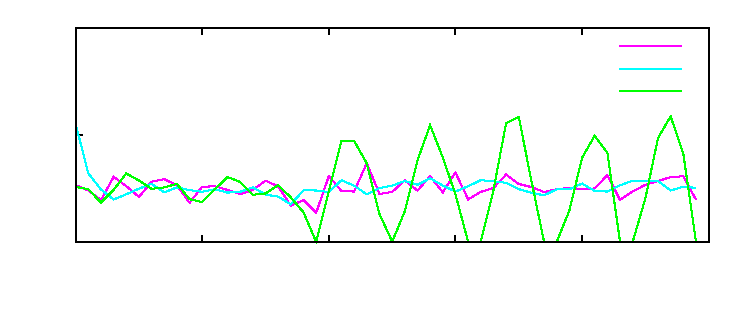
\includegraphics{esc/R5}}%
    \gplfronttext
  \end{picture}%
\endgroup
}
\caption{Ordering profile at $R3$}
\label{fig:esc:Order}
\end{figure}



In Figure \ref{fig:esc:R3}, we plot the inventory and the
back-order of  of the product $A$
at retailer $R3$. Note that the steady-state for product $A$ was
7.93. 

\begin{figure}[h]
\centering
\scriptsize
\resizebox{1\textwidth}{!}{% GNUPLOT: LaTeX picture with Postscript
\begingroup
  \makeatletter
  \providecommand\color[2][]{%
    \GenericError{(gnuplot) \space\space\space\@spaces}{%
      Package color not loaded in conjunction with
      terminal option `colourtext'%
    }{See the gnuplot documentation for explanation.%
    }{Either use 'blacktext' in gnuplot or load the package
      color.sty in LaTeX.}%
    \renewcommand\color[2][]{}%
  }%
  \providecommand\includegraphics[2][]{%
    \GenericError{(gnuplot) \space\space\space\@spaces}{%
      Package graphicx or graphics not loaded%
    }{See the gnuplot documentation for explanation.%
    }{The gnuplot epslatex terminal needs graphicx.sty or graphics.sty.}%
    \renewcommand\includegraphics[2][]{}%
  }%
  \providecommand\rotatebox[2]{#2}%
  \@ifundefined{ifGPcolor}{%
    \newif\ifGPcolor
    \GPcolorfalse
  }{}%
  \@ifundefined{ifGPblacktext}{%
    \newif\ifGPblacktext
    \GPblacktexttrue
  }{}%
  % define a \g@addto@macro without @ in the name:
  \let\gplgaddtomacro\g@addto@macro
  % define empty templates for all commands taking text:
  \gdef\gplbacktext{}%
  \gdef\gplfronttext{}%
  \makeatother
  \ifGPblacktext
    % no textcolor at all
    \def\colorrgb#1{}%
    \def\colorgray#1{}%
  \else
    % gray or color?
    \ifGPcolor
      \def\colorrgb#1{\color[rgb]{#1}}%
      \def\colorgray#1{\color[gray]{#1}}%
      \expandafter\def\csname LTw\endcsname{\color{white}}%
      \expandafter\def\csname LTb\endcsname{\color{black}}%
      \expandafter\def\csname LTa\endcsname{\color{black}}%
      \expandafter\def\csname LT0\endcsname{\color[rgb]{1,0,0}}%
      \expandafter\def\csname LT1\endcsname{\color[rgb]{0,1,0}}%
      \expandafter\def\csname LT2\endcsname{\color[rgb]{0,0,1}}%
      \expandafter\def\csname LT3\endcsname{\color[rgb]{1,0,1}}%
      \expandafter\def\csname LT4\endcsname{\color[rgb]{0,1,1}}%
      \expandafter\def\csname LT5\endcsname{\color[rgb]{1,1,0}}%
      \expandafter\def\csname LT6\endcsname{\color[rgb]{0,0,0}}%
      \expandafter\def\csname LT7\endcsname{\color[rgb]{1,0.3,0}}%
      \expandafter\def\csname LT8\endcsname{\color[rgb]{0.5,0.5,0.5}}%
    \else
      % gray
      \def\colorrgb#1{\color{black}}%
      \def\colorgray#1{\color[gray]{#1}}%
      \expandafter\def\csname LTw\endcsname{\color{white}}%
      \expandafter\def\csname LTb\endcsname{\color{black}}%
      \expandafter\def\csname LTa\endcsname{\color{black}}%
      \expandafter\def\csname LT0\endcsname{\color{black}}%
      \expandafter\def\csname LT1\endcsname{\color{black}}%
      \expandafter\def\csname LT2\endcsname{\color{black}}%
      \expandafter\def\csname LT3\endcsname{\color{black}}%
      \expandafter\def\csname LT4\endcsname{\color{black}}%
      \expandafter\def\csname LT5\endcsname{\color{black}}%
      \expandafter\def\csname LT6\endcsname{\color{black}}%
      \expandafter\def\csname LT7\endcsname{\color{black}}%
      \expandafter\def\csname LT8\endcsname{\color{black}}%
    \fi
  \fi
  \setlength{\unitlength}{0.0500bp}%
  \begin{picture}(7200.00,3024.00)%
    \gplgaddtomacro\gplbacktext{%
      \csname LTb\endcsname%
      \put(594,946){\makebox(0,0)[r]{\strut{} 0}}%
      \put(594,2155){\makebox(0,0)[r]{\strut{} 10}}%
      \put(828,484){\makebox(0,0){\strut{} 0}}%
      \put(1339,484){\makebox(0,0){\strut{} 10}}%
      \put(1850,484){\makebox(0,0){\strut{} 20}}%
      \put(2361,484){\makebox(0,0){\strut{} 30}}%
      \put(2872,484){\makebox(0,0){\strut{} 40}}%
      \put(3383,484){\makebox(0,0){\strut{} 50}}%
      \put(2054,154){\makebox(0,0){\strut{}Time}}%
    }%
    \gplgaddtomacro\gplfronttext{%
      \csname LTb\endcsname%
      \put(2396,2586){\makebox(0,0)[r]{\strut{}Inventory}}%
      \csname LTb\endcsname%
      \put(2396,2366){\makebox(0,0)[r]{\strut{}Backorder}}%
    }%
    \gplgaddtomacro\gplbacktext{%
      \csname LTb\endcsname%
      \put(4201,484){\makebox(0,0){\strut{} 0}}%
      \put(4661,484){\makebox(0,0){\strut{} 10}}%
      \put(5121,484){\makebox(0,0){\strut{} 20}}%
      \put(5582,484){\makebox(0,0){\strut{} 30}}%
      \put(6042,484){\makebox(0,0){\strut{} 40}}%
      \put(6502,484){\makebox(0,0){\strut{} 50}}%
      \put(6634,704){\makebox(0,0)[l]{\strut{} 0}}%
      \put(6634,1732){\makebox(0,0)[l]{\strut{} 10}}%
      \put(6634,2759){\makebox(0,0)[l]{\strut{} 20}}%
      \put(5305,154){\makebox(0,0){\strut{}Time}}%
    }%
    \gplgaddtomacro\gplfronttext{%
      \csname LTb\endcsname%
      \put(5779,2586){\makebox(0,0)[r]{\strut{}Customer demand}}%
      \csname LTb\endcsname%
      \put(5779,2366){\makebox(0,0)[r]{\strut{}Orders placed}}%
    }%
    \gplbacktext
    \put(0,0){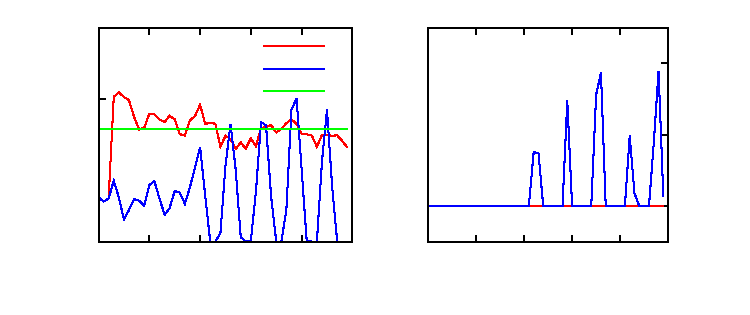
\includegraphics{R3}}%
    \gplfronttext
  \end{picture}%
\endgroup
}
\caption{Inventory and Backorder profile at $R3$}
\label{fig:esc:R3}
\end{figure}

Finally, in Table \ref{tab:esc:avgA}, we list the
average inventory at each node for products $A$ and $B$. Observe that
the average inventory at the nodes for the MPC policy is much closer
to the steady-state values, indicating that the MPC policy is
stabilizing. This example also illustrates the inherent robustness of
economic MPC as the controller was able to reject small variations in
demand around the nominal demand.

\begin{table}[h]
\caption{Average inventory for Product-A}
\label{tab:esc:avgA}
\begin{center}
\begin{tabular}{cccccccccc}\toprule
 &$M1$&$D1$&$D2$&$R1$&$R2$&$R3$&$R4$&$R5$\\ \midrule
MPC&58.01&17.48&12.36&0.34&5.43&7.71&0.26&3.44\\ 
Policy&82.91&10.70&6.02&0.011&1.39&3.21&0.23&5.47\\
\bottomrule 
\end{tabular}
\end{center}
\end{table}
\subsection{Scheduling model}
\label{sec:esc:multi:scheduling}
In the preceding sections, we did not consider the scheduling problem
at the manufacturing unit; instead, we approximated the production
delay using a constant production lead-time. In this section, we study
the economic MPC closed-loop performance for a supply chain which
includes a scheduling model for the manufacturing node.

We consider the same supply chain as in the previous section (Fig
\ref{fig:esc:lssc}), but with the following modification. The
manufacturing facility is assumed to have one unit $U$ which can
 make both products $A$ and $B$. The unit needs $3$ time units to make
$A$ via the task $\text{TA}$ and $2$ time units to make $B$ via the task
$\text{TB}$. In addition, there is changeover time of 1 unit whenever the
task is changed from $A$ to $B$ or vice-versa. 

Denote the set $\mathbf{I} = \set{\text{TA},\text{TB}}$,  $\text{PT}(i)$ as the
production lead time for each $i \in \mathbf{I}$ and $\text{CHT}(i,i')$ as
the changeover time between $i$ to $i'$. The scheduling constraints on
the manufacturing node can now be enforced by the following
inequalities (see \ref{sec:scheduling:example}):

\begin{alignat}{2}
&\sum_{i\in \mathbf{I}}\sum_{t' = t-\tau_i+1}^{t}W_{i,t'}+\sum_{i' \in
 \mathbf{I} \atop i' \neq i}\sum_{t'=t-\text{CHT}(i,i')+1}^{t}
Z_{i,i',t'} \leq 1 & \forall t \nonumber \\ 
&\sum_{t' = t-\tau_i+1}^{t} W_{i,t'} = Y_{i,t} & \forall t, \forall i
\in \mathbf{I} \nonumber\\
&X_{i,t} \geq Y_{i,t} & \forall t, \forall i \in \mathbf{I} \nonumber\\
&\sum_{i \in \mathbf{I}}X_{i,t} = 1 & \forall
t  \label{eq:esc:assign}\\ 
&Z_{i,i',t} \leq X_{i,t-1} &\forall t, \forall i \in \mathbf{I}, i' \in
\mathbf{I}, i' \neq i \nonumber\\
&Z_{i,i',t} \leq X_{i',t} &\forall t, \forall i \in \mathbf{I}, i' \in
\mathbf{I}, i'\neq i \nonumber \\
&Z_{i,i',t} \geq X_{i,t-1}+X_{i',t}-1 &\forall t, \forall i \in \mathbf{I}, i' \in
\mathbf{I}, i' \neq i \nonumber
\end{alignat}

To model the changeover time, we introduce three new binary variables $Z_{i,i',t},Y_{i,t}$ and
$X_{i,t}$. The binary variable $Z_{i,i',t}$ is 1 when a changeover is
effected from task $i$ to task $i'$ at time $t$. The binary variable
$Y_{i,t}$ is $1$ if the task $i$ was started during $[t-\tau_i,t]$. The
binary variable $X_{i,t}$ is 1 if the last task to be performed in the
unit before time $t$ was $i$.

In addition to these constraints, the batch-size is also controlled using
$W_{i,t}$ and the maximum and minimum batch-sizes. For the supply chain
studied, the maximum batch size was chosen to be $200$ for both the
products. The cost function corresponding to the new variables
included a cost to start a batch and a cost to effect a changeover
(see Table \ref{tab:esc:sched_prod}).

\begin{table*}
\caption{Production costs}
\label{tab:esc:sched_prod}
\begin{center}
\begin{tabular}{cc}\toprule
 &Cost \\ \midrule
Start a batch of TA & 10\\
Start a batch of TB & 6 \\
Changeover from TA to TB & 10\\
Changeover from TB to TA & 5\\
\bottomrule 
\end{tabular}
\end{center}
\end{table*}


Following the procedure outlined in
Chapter \ref{chap:scheduling}, we can write the supply
chain dynamics with the binary variables in the state space format
\eqref{eq:esc:model}. We denote the state space model of the
manufacturer scheduling problem as

\begin{equation}
x_M^+ = A_Mx_M + B_Mu_M + B_{d,M}u_{-M}
\end{equation}

in which $u_{-M}$ are the inputs of the other nodes in the supply chain, that is, the
shipping and ordering among $(D1,D2,R1 - R5)$ as well as the orders
placed by them to $M1$. The input $u_M$ consists of shipments sent by
the manufacturer to  the other nodes, and the binary decisions given
in \eqref{eq:esc:assign}. 

Therefore, we can easily write the whole supply chain dynamics model in
the state space form \eqref{eq:esc:model}. We only note that the
inputs now include the binary choices at the manufacturer and the
constraint set, instead of being just $x \in \mathbb{X}, u \in \mathbb{U}$,
becomes
\begin{gather}
\label{eq:esc:constraints}
 x \in \mathbb{X}, u \in \mathbb{U} \\
 \underline{b} \leq E_x x(t) + E_u u(t) \leq \overline{b}
\end{gather}

with the second inequality representing the assignment constraint
\eqref{eq:esc:assign} in the state space form.


We now define the periodic optimization problem that is used to find a
sub-optimal infinite horizon schedule and shipping/ordering policies
in response to the nominal demand given in Table \ref{tab:esc:nomdem}. In
the previous section, we found the steady-state shipping and ordering
so that the supply chain returns to the same state at the next
sampling instance. In this section, we find a periodic policy 
so that after $N_{p}$ sampling periods, the supply chain returns to the starting
state. The interpretation is that, if we observe the  nominal demands over
an infinite horizon, then we can remain feasible with the periodic
policy (by repeating it infinitely).
The optimization problem solved is \footnote{Note that we are solving
  a purely economic problem}:

\begin{alignat}{2}
\label{eq:esc:Pp}
\mathbb{P}_p:& \min_{\bu,x(0)}{\sum_{i=0}^{N_p-1}\ell_E(x(i),u(i),d_s(i))}& \nonumber \\
&\text{s.t.~} x(i+1) = Ax(i) + Bu(i)+B_dd_s(i),&i = \set{0,1,\ldots,N_p-1} \\
& \text{Constraints}\eqref{eq:esc:constraints}&i = \set{0,1,\ldots,N_p-1} \nonumber\\
& x(0) = x(N_p)& \nonumber\\
\end{alignat}
in which $N_p$ is the period.  We denote the solution to
\eqref{eq:esc:Pp} by $(\mathbf{u}_p^0,x(0)_p^0)$,
The solution to \eqref{eq:esc:Pp} gives us the periodic state-profile
\begin{equation}
\label{eq:esc:Xperiodic}
\mathbb{X}_p =  \set {x^0_p(0),x(1;x^0_p(0),\bu_p^0,\bd_s),\ldots,x(N_p;x^0_p(0),\bu_p^0,\bd_s) }
\end{equation}

In Figure \ref{fig:esc:gantt_ss}, we show the Gantt chart for the periodic
schedule with $N_p = 24$.

\begin{figure}
\centering
\scriptsize
\centering
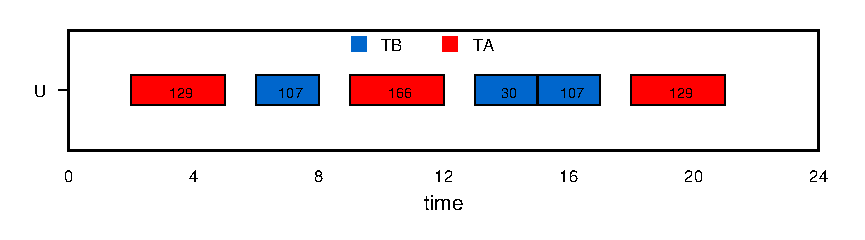
\includegraphics{esc/SS_gantt.pdf}
\caption{Periodic production schedule to respond to nominal demands}
\label{fig:esc:gantt_ss}

\label{fig:esc:ganttTNT1}
\begin{center}
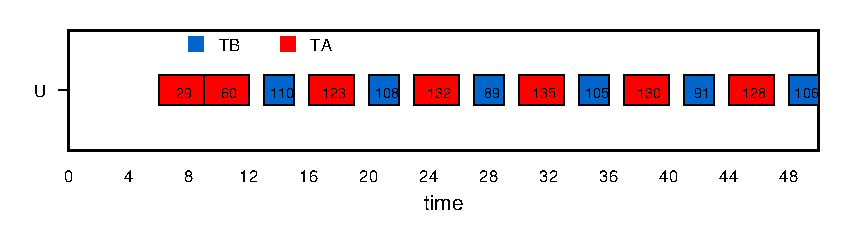
\includegraphics{esc/NTS_gantt.pdf}
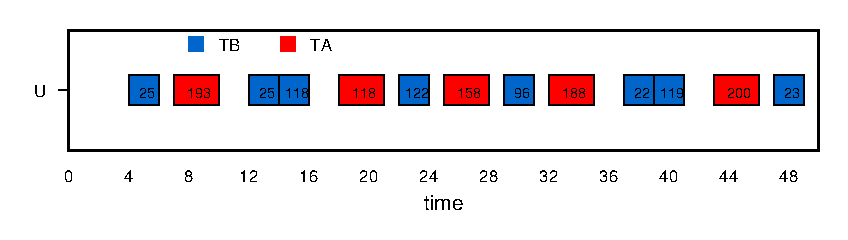
\includegraphics{esc/TS_gantt.pdf}
\caption{Production schedule for the MPC without terminal constraints that optimized
  \eqref{eq:esc:PbNT} (Top) compared with production schedule for the MPC
  with terminal constraints that optimized \eqref{eq:esc:PbT}. Note how larger batches are made for
  the problem with terminal constraints}
\end{center}
\end{figure}

\begin{figure}
\centering
\scriptsize
\resizebox{1\textwidth}{!}{% GNUPLOT: LaTeX picture with Postscript
\begingroup
  \makeatletter
  \providecommand\color[2][]{%
    \GenericError{(gnuplot) \space\space\space\@spaces}{%
      Package color not loaded in conjunction with
      terminal option `colourtext'%
    }{See the gnuplot documentation for explanation.%
    }{Either use 'blacktext' in gnuplot or load the package
      color.sty in LaTeX.}%
    \renewcommand\color[2][]{}%
  }%
  \providecommand\includegraphics[2][]{%
    \GenericError{(gnuplot) \space\space\space\@spaces}{%
      Package graphicx or graphics not loaded%
    }{See the gnuplot documentation for explanation.%
    }{The gnuplot epslatex terminal needs graphicx.sty or graphics.sty.}%
    \renewcommand\includegraphics[2][]{}%
  }%
  \providecommand\rotatebox[2]{#2}%
  \@ifundefined{ifGPcolor}{%
    \newif\ifGPcolor
    \GPcolortrue
  }{}%
  \@ifundefined{ifGPblacktext}{%
    \newif\ifGPblacktext
    \GPblacktexttrue
  }{}%
  % define a \g@addto@macro without @ in the name:
  \let\gplgaddtomacro\g@addto@macro
  % define empty templates for all commands taking text:
  \gdef\gplbacktext{}%
  \gdef\gplfronttext{}%
  \makeatother
  \ifGPblacktext
    % no textcolor at all
    \def\colorrgb#1{}%
    \def\colorgray#1{}%
  \else
    % gray or color?
    \ifGPcolor
      \def\colorrgb#1{\color[rgb]{#1}}%
      \def\colorgray#1{\color[gray]{#1}}%
      \expandafter\def\csname LTw\endcsname{\color{white}}%
      \expandafter\def\csname LTb\endcsname{\color{black}}%
      \expandafter\def\csname LTa\endcsname{\color{black}}%
      \expandafter\def\csname LT0\endcsname{\color[rgb]{1,0,0}}%
      \expandafter\def\csname LT1\endcsname{\color[rgb]{0,1,0}}%
      \expandafter\def\csname LT2\endcsname{\color[rgb]{0,0,1}}%
      \expandafter\def\csname LT3\endcsname{\color[rgb]{1,0,1}}%
      \expandafter\def\csname LT4\endcsname{\color[rgb]{0,1,1}}%
      \expandafter\def\csname LT5\endcsname{\color[rgb]{1,1,0}}%
      \expandafter\def\csname LT6\endcsname{\color[rgb]{0,0,0}}%
      \expandafter\def\csname LT7\endcsname{\color[rgb]{1,0.3,0}}%
      \expandafter\def\csname LT8\endcsname{\color[rgb]{0.5,0.5,0.5}}%
    \else
      % gray
      \def\colorrgb#1{\color{black}}%
      \def\colorgray#1{\color[gray]{#1}}%
      \expandafter\def\csname LTw\endcsname{\color{white}}%
      \expandafter\def\csname LTb\endcsname{\color{black}}%
      \expandafter\def\csname LTa\endcsname{\color{black}}%
      \expandafter\def\csname LT0\endcsname{\color{black}}%
      \expandafter\def\csname LT1\endcsname{\color{black}}%
      \expandafter\def\csname LT2\endcsname{\color{black}}%
      \expandafter\def\csname LT3\endcsname{\color{black}}%
      \expandafter\def\csname LT4\endcsname{\color{black}}%
      \expandafter\def\csname LT5\endcsname{\color{black}}%
      \expandafter\def\csname LT6\endcsname{\color{black}}%
      \expandafter\def\csname LT7\endcsname{\color{black}}%
      \expandafter\def\csname LT8\endcsname{\color{black}}%
    \fi
  \fi
  \setlength{\unitlength}{0.0500bp}%
  \begin{picture}(7200.00,3024.00)%
    \gplgaddtomacro\gplbacktext{%
      \csname LTb\endcsname%
      \put(946,714){\makebox(0,0)[r]{\strut{} 0}}%
      \put(946,919){\makebox(0,0)[r]{\strut{} 10}}%
      \put(946,1123){\makebox(0,0)[r]{\strut{} 20}}%
      \put(946,1328){\makebox(0,0)[r]{\strut{} 30}}%
      \put(946,1532){\makebox(0,0)[r]{\strut{} 40}}%
      \put(946,1737){\makebox(0,0)[r]{\strut{} 50}}%
      \put(946,1941){\makebox(0,0)[r]{\strut{} 60}}%
      \put(946,2146){\makebox(0,0)[r]{\strut{} 70}}%
      \put(946,2350){\makebox(0,0)[r]{\strut{} 80}}%
      \put(946,2555){\makebox(0,0)[r]{\strut{} 90}}%
      \put(946,2759){\makebox(0,0)[r]{\strut{} 100}}%
      \put(1078,484){\makebox(0,0){\strut{} 0}}%
      \put(2223,484){\makebox(0,0){\strut{} 10}}%
      \put(3368,484){\makebox(0,0){\strut{} 20}}%
      \put(4513,484){\makebox(0,0){\strut{} 30}}%
      \put(5658,484){\makebox(0,0){\strut{} 40}}%
      \put(6803,484){\makebox(0,0){\strut{} 50}}%
      \put(176,1731){\rotatebox{-270}{\makebox(0,0){\strut{}Backorder -Retailer}}}%
      \put(3940,154){\makebox(0,0){\strut{}Time}}%
    }%
    \gplgaddtomacro\gplfronttext{%
      \csname LTb\endcsname%
      \put(5816,2586){\makebox(0,0)[r]{\strut{}Without terminal constraint}}%
      \csname LTb\endcsname%
      \put(5816,2366){\makebox(0,0)[r]{\strut{}With terminal constraint}}%
    }%
    \gplbacktext
    \put(0,0){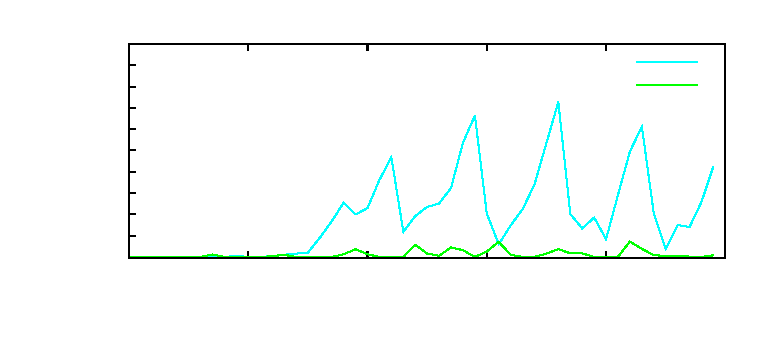
\includegraphics{BOprofile}}%
    \gplfronttext
  \end{picture}%
\endgroup
}
\caption{Combined backorder at all the retailer nodes}
\label{fig:esc:BOTNT}
\end{figure}

\subsubsection{Dynamic Response}
In this section, we show the dynamic response to a stochastic demand
signal.

We first consider the closed-loop solution, in which, at each sampling
time optimization problem \eqref{eq:esc:PbNT} is solved, and compare it
with the closed-loop solution in which the optimization problem
\eqref{eq:esc:PbT} is solved. In \eqref{eq:esc:PbT}, we force the final state
to lie on the periodic profile $\mathbb{X}_p$. Hence, at the end of
the planning horizon $N$, the supply-chain is at a state from which it
can respond to the nominal demand. In contrast, for the optimization
problem \eqref{eq:esc:PbNT}, the terminal state is chosen without
considering future demands that arrive after the planning horizon
$N$. Therefore, the solutions to \eqref{eq:esc:PbNT} have (i) fewer
production and (ii) lesser inventory at nodes. This leads to
increasing backorders when new demands are observed at the next
sampling time. In Figure \ref{fig:esc:BOTNT}, we compare the backorders
observed in the closed-loop when the MPC optimizer solved
\eqref{eq:esc:PbNT} and \eqref{eq:esc:PbT}. In Figure \ref{fig:esc:ganttTNT1}, we
show the Gantt chart for the implemented schedule by the two MPCs. The
planning horizon used was $N = 12$. Note that, under the presence of
persistent disturbance (that is different from the nominal
disturbance), the MPC design has to be robust
\citep[Ch 3.]{rawlings:mayne:2009}. In this example, we have not
designed robust-MPC but instead the results show the inherent-robustness of
nominal MPC to reject small deviations from the nominal
demand. 
 
\begin{alignat}{2}
\label{eq:esc:PbNT}
\mathbb{P}_N(x):& \min_{\bu}
{\sum_{i=0}^{N-1}\ell_E(x(j),u(j),d(j))}& \nonumber \\
&\text{s.t.~} x(j+1) = Ax(j) + Bu(j)+B_dd_s(j),&j = \set{0,1,\ldots,N-1}\\\
& \text{Constraints}\eqref{eq:esc:constraints}&j = \set{0,1,\ldots,N-1} \nonumber\\
& x(0) = x \nonumber\\
\end{alignat}

\begin{alignat}{2}
\label{eq:esc:PbT}
\mathbb{P}_N(x):& \min_{\bu}
{\sum_{i=0}^{N-1}\ell_E(x(j),u(j),d(j))}& \nonumber \\
&\text{s.t.~} x(j+1) = Ax(j) + Bu(j)+B_dd_s(j),&j = \set{0,1,\ldots,N-1}\\\
& \text{Constraints}\eqref{eq:esc:constraints}&j = \set{0,1,\ldots,N-1} \nonumber\\
& x(0) = x \nonumber\\
& x(N) \in \mathbb{X}_P
\end{alignat}








\chapter{Conclusions and Future work}
\label{chap:conclusions}
We conclude with a summary of contributions and suggest possible
directions for further research.

\section*{Contributions}

\paragraph{Cooperative MPC for linear systems:} In Chapter
\ref{chap:mpc} we provided an overview of cooperative MPC for linear
systems. The main contribution in Chapter \ref{chap:mpc} were (i) The
extension of the class of systems for which cooperative MPC is
applicable to all centralized  stabilizable systems and, (ii) Tube based robust
cooperative MPC to avoid centralized restarts if the warm start fails.

\paragraph{State-space models for scheduling:} In Chapter
\ref{chap:scheduling}, we provided a state-space model for
scheduling. We expressed the scheduling problem as a dynamic problem
for iterative scheduling. We also modeled a variety of scheduling
disturances so that rescheduling occurs ``naturally'' in iterative
scheduling. Finally, we used tools from MPC to demonstrate design of closed-loop scheduling
problems with guaranteed recursive feasibility.

\paragraph{MPC for supply chains:} A goal of this thesis was to use
MPC as a general purpose tool for enterprise wide optimization. We
demonstrated MPC design for dynamic supply chain models. The main
contribution of this thesis is to complement the research in 
MPC/ Rolling horizon optimization frameworks for supply chain
management by (i) showing the desirable properties of algorithms that
guarantee closed-loop stability and, (ii) demonstrating the design of
such control policies for supply chains.  The main message of the thesis  is
that future researchers should appreciate the importance of
considering the closed-loop dynamics of the supply chain as a result
of the input actions taken. 
\begin{enumerate}
\item In order to appeal to the distributed nature of decision making in supply
chains, we demonstrated cooperative MPC for supply chains in which
each node makes its local decisions but with a global vision in
Chapter \ref{chap:sc}. We
proposed a new cooperative MPC iteration scheme which closely
resembles the current decision making hierarchy in linear supply
chains.
\item Since supply chains directly optimize the economics, we
  demonstrated design of Economic MPC for supply chains in Chapter
  \ref{chap:esc}. We proposed a multiobjective stage cost, that not
  only accounts for supply chain costs, but also for supply chain
  risks. The supply chain is  stabilized at a steady-state that
  reflects the managers' choice, i.e., risk seeking or risk averse.
\end{enumerate}

\paragraph{Integration of scheduling and control:} We demonstrated a
supply chain example with an integrated scheduling model for the
manufacturing plant. We showed the integration of the MPC design tools from
Chapter \ref{chap:mpc} and Chapter \ref{chap:esc} along with the
state-space scheduling model from Chapter \ref{chap:scheduling} to
guarantee recursive feasibility for the integrated supply chain
model. We also showed the inherent robustness of the proposed approach
to small deviations from the nominal demand.

\section*{Future work}

\paragraph{Terminal conditions for the scheduling problem:}
In Chapter \ref{chap:scheduling}, we showed recursive feasibility by
using a cyclic schedule as the terminal condition. In many cases, we
might not be able to find any cyclic schedule for the scheduling
problem. In such cases, we have to find other suitable terminal
conditions. One such idea that we are currently exploring is to find
safety constraints on inventory from a scheduling point of view.
Methods of finding terminal conditions for the scheduling problem is
an important area for future research.
\paragraph{Hybrid control theory:}
The scheduling state space model comprises both of continuous
variables (like the inventories, batch sizes, etc.) and discrete variables
(like assignment, changeover etc.). For such systems, we need to study
the stability theory for hybrid systems. There are methods that have
been developed for hybrid dynamic systems consisting of both time and
event driven dynamics \citep{bemporad:morari:1999,
  morari:baotic:borrelli:2003} etc. More recently, Lyapunov stability
theory for hybrid dynamic systems also have been studied
\citep{lazar:heemels:2009,lazar:heemels:teel:2009}. Application and
development  of hybrid theory to prove stability of scheduling models
is a challenging research problem.
\paragraph{Impact of forecast:}
Supply chains are described as ``pull'' systems because the  dynamics
is activated when the customer pulls products from the 
supply chain. As such, the supply chain is sensitive to customer
demands, price signals, etc. MPC theory has been mostly built around
dynamic models trying to ``reject'' external disturbances ( \eg the
nominal case is when there is no disturbance affecting the
system). The impact of demand/ price forecast 
the supply chain steady state; performance, etc. are yet to be studied. 
\paragraph{ Robust terminal conditions:}
In this thesis, we developed  algorithms based on a nominal demand
signal. That is, the stability and convergence guarantees; and
specially, the design of terminal
region/ constraints were based on the nominal demand. In practice, it
is desirable to design the terminal constraint so that we are robust
to some known distribution of demands. Design of such terminal regions
and integration with MPC technology remains an avenue of future work. 
\paragraph{Cooperative game theory:} The cooperative MPC tools have
been developed for process industries to coordinate multiple MPC's in
a single plant. Therefore, it is reasonable to assume that all the
subsystems can share models and objectives with each-other. In a
supply chain, however,the nodes could
be owned by different companies. Hence, we need to study the incentives to cooperate
from a cooperative game theory point of view. 
\paragraph{Implementation:} The ultimate test for any new tool is
practical implementation. An avenue of future research is the
implementation of the tools described in this thesis for a large scale
supply chain with real data. Not only, would such a study help
validate the idea of using MPC for supply chains, it would also help
us uncover new research topics.


\bibliographystyle{plainnat}
\bibliography{abbreviations,articles,books,proceedings,unpub}

%\begin{appendices}
%\end{appendices}
\newpage
\begin{umiabstract}
  \pagestyle{empty}
  \addtocounter{page}{-1}
  A supply chain is a network of facilities and distribution options
that performs the functions of procuring raw materials, transforming
them to products and distributing the finished products to the
customers. The modern supply chain is a highly interconnected network
of facilities that are spread over multiple locations and handle
multiple products. In a highly competitive global
environment, optimal day-to-day operations of supply chains is
essential.

To facilitate optimal operations in supply chains, we propose the use of
Model Predictive Control (MPC) for supply chains. We develop:  

\begin{itemize}
\item A new cooperative MPC algorithm that can stabilize any
  centralized stabilizable system
\item A new algorithm for robust cooperative MPC
\item A state space model for the chemical production scheduling problem
\end{itemize}

We use the new tools and algorithms to design model predictive
controllers for supply chain models. We demonstrate:

\begin{itemize}
\item {\textbf{Cooperative control for supply chains}}: In cooperative MPC, each node makes its
  decisions by considering the effects of their decisions on the
  entire supply chain. We show that the cooperative controller can
  perform better than the noncooperative and decentralized  controller
  and can reduce the  bullwhip effect in the supply chain. 

\item {\textbf{Centralized economic control}}: We propose a new multiobjective
  stage cost that captures both the economics and risk at a node,
  using a weighted sum of an economic stage cost and a tracking stage
  cost. We use Economic MPC theory \citep{amrit:rawlings:angeli:2011} to design
  closed-loop stable controllers for the supply chain. 

\item {\textbf{Integrated supply chain}}: We show an example of integrating
  inventory control with production scheduling using the tools
  developed in this thesis. We develop simple terminal conditions to
  show recursive feasibility of such integrated control schemes.
\end{itemize}


\end{umiabstract}

\end{document}
